%&preformat-disser
\RequirePackage[l2tabu,orthodox]{nag} % Раскомментировав, можно в логе получать рекомендации относительно правильного использования пакетов и предупреждения об устаревших и нерекомендуемых пакетах
% Формат А4, 14pt (ГОСТ Р 7.0.11-2011, 5.3.6)
\documentclass[a4paper,14pt,oneside,openany]{memoir}

%%%%%%%%%%%%%%%%%%%%%%%%%%%%%%%%%%%%%%%%%%%%%%%%%%%%%%%%%%%%%%%%%%%%%%%%%%%%%%%%
%%%% Файл упрощённых настроек шаблона, общих для диссертации и автореферата %%%%
%%%%%%%%%%%%%%%%%%%%%%%%%%%%%%%%%%%%%%%%%%%%%%%%%%%%%%%%%%%%%%%%%%%%%%%%%%%%%%%%

%%% Режим черновика %%%
\makeatletter
\@ifundefined{c@draft}{
  \newcounter{draft}
  \setcounter{draft}{0}  % 0 --- чистовик (максимальное соблюдение ГОСТ)
                         % 1 --- черновик (отклонения от ГОСТ, но быстрая
                         %       сборка итоговых PDF)
}{}
\makeatother

%%% Пометки в тексте %%%
\makeatletter
\@ifundefined{c@showmarkup}{
  \newcounter{showmarkup}
  \setcounter{showmarkup}{0}  % 0 --- скрыть пометки
                              % 1 --- показывать пометки
}{}
\makeatother

%%% Использование в pdflatex шрифтов не по-умолчанию %%%
\makeatletter
\@ifundefined{c@usealtfont}{
  \newcounter{usealtfont}
  \setcounter{usealtfont}{1}    % 0 --- шрифты на базе Computer Modern
                                % 1 --- использовать пакет pscyr, при его
                                %       наличии
                                % 2 --- использовать пакет XCharter, при наличии
                                %       подходящей версии
}{}
\makeatother

%%% Использование в xelatex и lualatex семейств шрифтов %%%
\makeatletter
\@ifundefined{c@fontfamily}{
  \newcounter{fontfamily}
  \setcounter{fontfamily}{1}  % 0 --- CMU семейство. Используется как fallback;
                              % 1 --- Шрифты от MS (Times New Roman и компания)
                              % 2 --- Семейство Liberation
}{}
\makeatother

%%% Библиография %%%
\makeatletter
\@ifundefined{c@bibliosel}{
  \newcounter{bibliosel}
  \setcounter{bibliosel}{1}   % 0 --- встроенная реализация с загрузкой файла
                              %       через движок bibtex8;
                              % 1 --- реализация пакетом biblatex через движок
                              %       biber
}{}
\makeatother

%%% Вывод типов ссылок в библиографии %%%
\makeatletter
\@ifundefined{c@mediadisplay}{
  \newcounter{mediadisplay}
  \setcounter{mediadisplay}{1}   % 0 --- не делать ничего; надписи [Текст] и
                                 %       [Эл. ресурс] будут выводиться только в ссылках с
                                 %       заполненным полем `media`;
                                 % 1 --- автоматически добавлять надпись [Текст] к ссылкам с
                                 %       незаполненным полем `media`; таким образом, у всех
                                 %       источников будет указан тип, что соответствует
                                 %       требованиям ГОСТ
                                 % 2 --- автоматически удалять надписи [Текст], [Эл. Ресурс] и др.;
                                 %       не соответствует ГОСТ
                                 % 3 --- автоматически удалять надпись [Текст];
                                 %       не соответствует ГОСТ
                                 % 4 --- автоматически удалять надпись [Эл. Ресурс];
                                 %       не соответствует ГОСТ
}{}
\makeatother

%%% Предкомпиляция tikz рисунков для ускорения работы %%%
\makeatletter
\@ifundefined{c@imgprecompile}{
  \newcounter{imgprecompile}
  \setcounter{imgprecompile}{0}   % 0 --- без предкомпиляции;
                                  % 1 --- пользоваться предварительно
                                  %       скомпилированными pdf вместо генерации
                                  %       заново из tikz
}{}
\makeatother
            % общие настройки шаблона
%%% Проверка используемого TeX-движка %%%
\newif\ifxetexorluatex   % определяем новый условный оператор (http://tex.stackexchange.com/a/47579)
\ifxetex
    \xetexorluatextrue
\else
    \ifluatex
        \xetexorluatextrue
    \else
        \xetexorluatexfalse
    \fi
\fi

\newif\ifsynopsis           % Условие, проверяющее, что документ --- автореферат

\usepackage{etoolbox}[2015/08/02]   % Для продвинутой проверки разных условий
\providebool{presentation}

\usepackage{comment}    % Позволяет убирать блоки текста (добавляет
                        % окружение comment и команду \excludecomment)

%%% Поля и разметка страницы %%%
\usepackage{pdflscape}  % Для включения альбомных страниц
\usepackage{geometry}   % Для последующего задания полей

%%% Математические пакеты %%%
\usepackage{amsthm,amsmath,amscd}   % Математические дополнения от AMS
\usepackage{amsfonts,amssymb}       % Математические дополнения от AMS
\usepackage{mathtools}              % Добавляет окружение multlined
\usepackage{xfrac}                  % Красивые дроби
\usepackage[
    locale = DE,
    list-separator       = {;\,},
    list-final-separator = {;\,},
    list-pair-separator  = {;\,},
    list-units           = single,
    range-units          = single,
    range-phrase={\text{\ensuremath{-}}},
    % quotient-mode        = fraction, % красивые дроби могут не соответствовать ГОСТ
    fraction-function    = \sfrac,
    separate-uncertainty,
    ]{siunitx}                      % Размерности SI
\sisetup{inter-unit-product = \ensuremath{{}\cdot{}}}

% Кириллица в нумерации subequations
% Для правильной работы требуется выполнение сразу после загрузки пакетов
\patchcmd{\subequations}{\def\theequation{\theparentequation\alph{equation}}}
{\def\theequation{\theparentequation\asbuk{equation}}}
{\typeout{subequations patched}}{\typeout{subequations not patched}}

%%%% Установки для размера шрифта 14 pt %%%%
%% Формирование переменных и констант для сравнения (один раз для всех подключаемых файлов)%%
%% должно располагаться до вызова пакета fontspec или polyglossia, потому что они сбивают его работу
\newlength{\curtextsize}
\newlength{\bigtextsize}
\setlength{\bigtextsize}{13.9pt}

\makeatletter
%\show\f@size    % неплохо для отслеживания, но вызывает стопорение процесса,
                 % если документ компилируется без команды  -interaction=nonstopmode
\setlength{\curtextsize}{\f@size pt}
\makeatother

%%% Кодировки и шрифты %%%
\ifxetexorluatex
    \ifpresentation
        \providecommand*\autodot{} % quick fix for polyglossia 1.50
    \fi
    \PassOptionsToPackage{no-math}{fontspec}    % https://tex.stackexchange.com/a/26295/104425
    \usepackage{polyglossia}[2014/05/21]        % Поддержка многоязычности
                                        % (fontspec подгружается автоматически)
\else
   %%% Решение проблемы копирования текста в буфер кракозябрами
    \ifnumequal{\value{usealtfont}}{0}{}{
        \input glyphtounicode.tex
        \input glyphtounicode-cmr.tex %from pdfx package
        \pdfgentounicode=1
    }
    \usepackage{cmap}   % Улучшенный поиск русских слов в полученном pdf-файле
    \ifnumequal{\value{usealtfont}}{2}{}{
        \defaulthyphenchar=127  % Если стоит до fontenc, то переносы
                                % не впишутся в выделяемый текст при
                                % копировании его в буфер обмена
    }
    \usepackage{textcomp}
    \usepackage[T1,T2A]{fontenc}                    % Поддержка русских букв
    \ifnumequal{\value{usealtfont}}{1}{% Используется pscyr, при наличии
        \IfFileExists{pscyr.sty}{\usepackage{pscyr}}{}  % Подключение pscyr
    }{}
    \usepackage[utf8]{inputenc}[2014/04/30]         % Кодировка utf8
    \usepackage[english, russian]{babel}[2014/03/24]% Языки: русский, английский
    \makeatletter\AtBeginDocument{\let\@elt\relax}\makeatother % babel 3.40 fix
    \ifnumequal{\value{usealtfont}}{2}{
        % http://dxdy.ru/post1238763.html#p1238763
        \usepackage[scaled=0.914]{XCharter}[2017/12/19] % Подключение русифицированных шрифтов XCharter
        \usepackage[charter, vvarbb, scaled=1.048]{newtxmath}[2017/12/14]
        \ifpresentation
        \else
            \setDisplayskipStretch{-0.078}
        \fi
    }{}
\fi

%%% Оформление абзацев %%%
\ifpresentation
\else
    \indentafterchapter     % Красная строка после заголовков типа chapter
    \usepackage{indentfirst}
\fi

%%% Цвета %%%
\ifpresentation
\else
    \usepackage[dvipsnames, table, hyperref]{xcolor} % Совместимо с tikz
\fi

%%% Таблицы %%%
\usepackage{longtable,ltcaption} % Длинные таблицы
\usepackage{multirow,makecell}   % Улучшенное форматирование таблиц
\usepackage{tabu, tabulary}      % таблицы с автоматически подбирающейся
                                 % шириной столбцов (tabu обязательно
                                 % до hyperref вызывать)
\usepackage{threeparttable}      % автоматический подгон ширины подписи таблицы

%%% Общее форматирование
\usepackage{soulutf8}% Поддержка переносоустойчивых подчёркиваний и зачёркиваний
\usepackage{icomma}  % Запятая в десятичных дробях

%%% Оптимизация расстановки переносов и длины последней строки абзаца
\IfFileExists{impnattypo.sty}{% проверка установленности пакета impnattypo
    \ifluatex
        \ifnumequal{\value{draft}}{1}{% Черновик
            \usepackage[hyphenation, lastparline, nosingleletter, homeoarchy,
            rivers, draft]{impnattypo}
        }{% Чистовик
            \usepackage[hyphenation, lastparline, nosingleletter]{impnattypo}
        }
    \else
        \usepackage[hyphenation, lastparline]{impnattypo}
    \fi
}{}

%% Векторная графика

\usepackage{tikz}                   % Продвинутый пакет векторной графики
\usetikzlibrary{chains}             % Для примера tikz рисунка
\usetikzlibrary{shapes.geometric}   % Для примера tikz рисунка
\usetikzlibrary{shapes.symbols}     % Для примера tikz рисунка
\usetikzlibrary{arrows}             % Для примера tikz рисунка

%%% Гиперссылки %%%
\usepackage{hyperref}[2012/11/06]

%%% Изображения %%%
\usepackage{graphicx}[2014/04/25]   % Подключаем пакет работы с графикой
\usepackage{caption}                % Подписи рисунков и таблиц
\usepackage{subcaption}             % Подписи подрисунков и подтаблиц
\usepackage{pdfpages}               % Добавление внешних pdf файлов

%%% Счётчики %%%
\usepackage{aliascnt}
\usepackage[figure,table]{totalcount}   % Счётчик рисунков и таблиц
\usepackage{totcount}   % Пакет создания счётчиков на основе последнего номера
                        % подсчитываемого элемента (может требовать дважды
                        % компилировать документ)
\usepackage{totpages}   % Счётчик страниц, совместимый с hyperref (ссылается
                        % на номер последней страницы). Желательно ставить
                        % последним пакетом в преамбуле

%%% Продвинутое управление групповыми ссылками (пока только формулами) %%%
\ifpresentation
\else
    \usepackage[russian]{cleveref} % cleveref имеет сложности со считыванием
    % языка из babel. Такое решение русификации вывода выбрано вместо
    % определения в documentclass из опасности что-то лишнее передать во все
    % остальные пакеты, включая библиографию.

    % Добавление возможности использования пробелов в \labelcref
    % https://tex.stackexchange.com/a/340502/104425
    \usepackage{kvsetkeys}
    \makeatletter
    \let\org@@cref\@cref
    \renewcommand*{\@cref}[2]{%
        \edef\process@me{%
            \noexpand\org@@cref{#1}{\zap@space#2 \@empty}%
        }\process@me
    }
    \makeatother
\fi

\usepackage{placeins} % для \FloatBarrier

\ifnumequal{\value{draft}}{1}{% Черновик
    \usepackage[firstpage]{draftwatermark}
    \SetWatermarkText{DRAFT}
    \SetWatermarkFontSize{14pt}
    \SetWatermarkScale{15}
    \SetWatermarkAngle{45}
}{}

%%% Цитата, не приводимая в автореферате:
% возможно, актуальна только для biblatex
%\newcommand{\citeinsynopsis}[1]{\ifsynopsis\else ~\cite{#1} \fi}

% если текущий процесс запущен библиотекой tikz-external, то прекомпиляция должна быть включена
\ifdefined\tikzexternalrealjob
    \setcounter{imgprecompile}{1}
\fi

\ifnumequal{\value{imgprecompile}}{1}{% Только если у нас включена предкомпиляция
    \usetikzlibrary{external}   % подключение возможности предкомпиляции
    \tikzexternalize[prefix=images/cache/,optimize command away=\includepdf] % activate! % здесь можно указать отдельную папку для скомпилированных файлов
    \ifxetex
        \tikzset{external/up to date check={diff}}
    \fi
}{}
         % Пакеты общие для диссертации и автореферата
\synopsisfalse                      % Этот документ --- не автореферат
%%% Прикладные пакеты %%%
%\usepackage{calc}               % Пакет для расчётов параметров, например длины

%%% Для добавления Стр. над номерами страниц в оглавлении
%%% http://tex.stackexchange.com/a/306950
\usepackage{afterpage}

%%% Списки %%%
\usepackage{enumitem}
    % Пакеты для диссертации
\usepackage{fr-longtable}    %ради \endlasthead

% Листинги с исходным кодом программ
\usepackage{fancyvrb}
\usepackage{listings}
\lccode`\~=0\relax %Без этого хака из-за особенностей пакета listings перестают работать конструкции с \MakeLowercase и т. п. в (xe|lua)latex

% Русская традиция начертания греческих букв
\usepackage{upgreek} % прямые греческие ради русской традиции

%%% Микротипографика
%\ifnumequal{\value{draft}}{0}{% Только если у нас режим чистовика
%    \usepackage[final, babel, shrink=45]{microtype}[2016/05/14] % улучшает представление букв и слов в строках, может помочь при наличии отдельно висящих слов
%}{}

% Отметка о версии черновика на каждой странице
% Чтобы работало надо в своей локальной копии по инструкции
% https://www.ctan.org/pkg/gitinfo2 создать небходимые файлы в папке
% ./git/hooks
% If you’re familiar with tweaking git, you can probably work it out for
% yourself. If not, I suggest you follow these steps:
% 1. First, you need a git repository and working tree. For this example,
% let’s suppose that the root of the working tree is in ~/compsci
% 2. Copy the file post-xxx-sample.txt (which is in the same folder of
% your TEX distribution as this pdf) into the git hooks directory in your
% working copy. In our example case, you should end up with a file called
% ~/compsci/.git/hooks/post-checkout
% 3. If you’re using a unix-like system, don’t forget to make the file executable.
% Just how you do this is outside the scope of this manual, but one
% possible way is with commands such as this:
% chmod g+x post-checkout.
% 4. Test your setup with “git checkout master” (or another suitable branch
% name). This should generate copies of gitHeadInfo.gin in the directories
% you intended.
% 5. Now make two more copies of this file in the same directory (hooks),
% calling them post-commit and post-merge, and you’re done. As before,
% users of unix-like systems should ensure these files are marked as
% executable.
\ifnumequal{\value{draft}}{1}{% Черновик
   \IfFileExists{.git/gitHeadInfo.gin}{
      \usepackage[mark,pcount]{gitinfo2}
      \renewcommand{\gitMark}{rev.\gitAbbrevHash\quad\gitCommitterEmail\quad\gitAuthorIsoDate}
      \renewcommand{\gitMarkFormat}{\rmfamily\color{Gray}\small\bfseries}
   }{}
}{}   % Пакеты для специфических пользовательских задач

%%%%%%%%%%%%%%%%%%%%%%%%%%%%%%%%%%%%%%%%%%%%%%%%%%%%%%
%%%% Файл упрощённых настроек шаблона диссертации %%%%
%%%%%%%%%%%%%%%%%%%%%%%%%%%%%%%%%%%%%%%%%%%%%%%%%%%%%%

%%% Инициализирование переменных, не трогать!  %%%
\newcounter{intvl}
\newcounter{otstup}
\newcounter{contnumeq}
\newcounter{contnumfig}
\newcounter{contnumtab}
\newcounter{pgnum}
\newcounter{chapstyle}
\newcounter{headingdelim}
\newcounter{headingalign}
\newcounter{headingsize}
%%%%%%%%%%%%%%%%%%%%%%%%%%%%%%%%%%%%%%%%%%%%%%%%%%%%%%

%%% Область упрощённого управления оформлением %%%

%% Интервал между заголовками и между заголовком и текстом %%
% Заголовки отделяют от текста сверху и снизу
% тремя интервалами (ГОСТ Р 7.0.11-2011, 5.3.5)
\setcounter{intvl}{3}               % Коэффициент кратности к размеру шрифта

%% Отступы у заголовков в тексте %%
\setcounter{otstup}{0}              % 0 --- без отступа; 1 --- абзацный отступ

%% Нумерация формул, таблиц и рисунков %%
% Нумерация формул
\setcounter{contnumeq}{0}   % 0 --- пораздельно (во введении подряд,
                            %       без номера раздела);
                            % 1 --- сквозная нумерация по всей диссертации
% Нумерация рисунков
\setcounter{contnumfig}{0}  % 0 --- пораздельно (во введении подряд,
                            %       без номера раздела);
                            % 1 --- сквозная нумерация по всей диссертации
% Нумерация таблиц
\setcounter{contnumtab}{1}  % 0 --- пораздельно (во введении подряд,
                            %       без номера раздела);
                            % 1 --- сквозная нумерация по всей диссертации

%% Оглавление %%
\setcounter{pgnum}{1}       % 0 --- номера страниц никак не обозначены;
                            % 1 --- Стр. над номерами страниц (дважды
                            %       компилировать после изменения настройки)
\settocdepth{subsection}    % до какого уровня подразделов выносить в оглавление
\setsecnumdepth{subsection} % до какого уровня нумеровать подразделы


%% Текст и форматирование заголовков %%
\setcounter{chapstyle}{1}     % 0 --- разделы только под номером;
                              % 1 --- разделы с названием "Глава" перед номером
\setcounter{headingdelim}{1}  % 0 --- номер отделен пропуском в 1em или \quad;
                              % 1 --- номера разделов и приложений отделены
                              %       точкой с пробелом, подразделы пропуском
                              %       без точки;
                              % 2 --- номера разделов, подразделов и приложений
                              %       отделены точкой с пробелом.

%% Выравнивание заголовков в тексте %%
\setcounter{headingalign}{0}  % 0 --- по центру;
                              % 1 --- по левому краю

%% Размеры заголовков в тексте %%
\setcounter{headingsize}{0}   % 0 --- по ГОСТ, все всегда 14 пт;
                              % 1 --- пропорционально изменяющийся размер
                              %       в зависимости от базового шрифта

%% Подпись таблиц %%

% Смещение строк подписи после первой строки
\newcommand{\tabindent}{0cm}

% Тип форматирования заголовка таблицы:
% plain --- название и текст в одной строке
% split --- название и текст в разных строках
\newcommand{\tabformat}{plain}

%%% Настройки форматирования таблицы `plain`

% Выравнивание по центру подписи, состоящей из одной строки:
% true  --- выравнивать
% false --- не выравнивать
\newcommand{\tabsinglecenter}{false}

% Выравнивание подписи таблиц:
% justified   --- выравнивать как обычный текст («по ширине»)
% centering   --- выравнивать по центру
% centerlast  --- выравнивать по центру только последнюю строку
% centerfirst --- выравнивать по центру только первую строку (не рекомендуется)
% raggedleft  --- выравнивать по правому краю
% raggedright --- выравнивать по левому краю
\newcommand{\tabjust}{justified}

% Разделитель записи «Таблица #» и названия таблицы
\newcommand{\tablabelsep}{~\cyrdash\ }

%%% Настройки форматирования таблицы `split`

% Положение названия таблицы:
% \centering   --- выравнивать по центру
% \raggedleft  --- выравнивать по правому краю
% \raggedright --- выравнивать по левому краю
\newcommand{\splitformatlabel}{\raggedleft}

% Положение текста подписи:
% \centering   --- выравнивать по центру
% \raggedleft  --- выравнивать по правому краю
% \raggedright --- выравнивать по левому краю
\newcommand{\splitformattext}{\raggedright}

%% Подпись рисунков %%
%Разделитель записи «Рисунок #» и названия рисунка
\newcommand{\figlabelsep}{~\cyrdash\ }  % (ГОСТ 2.105, 4.3.1)
                                        % "--- здесь не работает

%%% Цвета гиперссылок %%%
% Latex color definitions: http://latexcolor.com/
\definecolor{linkcolor}{rgb}{0.9,0,0}
\definecolor{citecolor}{rgb}{0,0.6,0}
\definecolor{urlcolor}{rgb}{0,0,1}
%\definecolor{linkcolor}{rgb}{0,0,0} %black
%\definecolor{citecolor}{rgb}{0,0,0} %black
%\definecolor{urlcolor}{rgb}{0,0,0} %black
      % Упрощённые настройки шаблона

% Новые переменные, которые могут использоваться во всём проекте
% ГОСТ 7.0.11-2011
% 9.2 Оформление текста автореферата диссертации
% 9.2.1 Общая характеристика работы включает в себя следующие основные структурные
% элементы:
% актуальность темы исследования;
\newcommand{\actualityTXT}{Актуальность темы.}
% степень ее разработанности;
\newcommand{\progressTXT}{Степень разработанности темы.}
% цели и задачи;
\newcommand{\aimTXT}{Целью}
\newcommand{\tasksTXT}{задачи}
% научную новизну;
\newcommand{\noveltyTXT}{Научная новизна:}
% теоретическую и практическую значимость работы;
%\newcommand{\influenceTXT}{Теоретическая и практическая значимость}
% или чаще используют просто
\newcommand{\influenceTXT}{Практическая значимость}
% методологию и методы исследования;
\newcommand{\methodsTXT}{Методология и методы исследования.}
% положения, выносимые на защиту;
\newcommand{\defpositionsTXT}{Основные положения, выносимые на~защиту:}
% степень достоверности и апробацию результатов.
\newcommand{\reliabilityTXT}{Достоверность}
\newcommand{\probationTXT}{Апробация работы.}

\newcommand{\contributionTXT}{Личный вклад.}
\newcommand{\publicationsTXT}{Публикации.}


%%% Заголовки библиографии:

% для автореферата:
\newcommand{\bibtitleauthor}{Публикации автора по теме диссертации}

% для стиля библиографии `\insertbiblioauthorgrouped`
\newcommand{\bibtitleauthorvak}{В изданиях из списка ВАК РФ}
\newcommand{\bibtitleauthorscopus}{В изданиях, входящих в международную базу цитирования Scopus}
\newcommand{\bibtitleauthorwos}{В изданиях, входящих в международную базу цитирования Web of Science}
\newcommand{\bibtitleauthorother}{В прочих изданиях}
\newcommand{\bibtitleauthorconf}{В сборниках трудов конференций}
\newcommand{\bibtitleauthorpatent}{Зарегистрированные патенты}
\newcommand{\bibtitleauthorprogram}{Зарегистрированные программы для ЭВМ}

% для стиля библиографии `\insertbiblioauthorimportant`:
\newcommand{\bibtitleauthorimportant}{Наиболее значимые \protect\MakeLowercase\bibtitleauthor}

% для списка литературы в диссертации и списка чужих работ в автореферате:
\newcommand{\bibtitlefull}{Список литературы} % (ГОСТ Р 7.0.11-2011, 4)
         % Новые переменные, для всего проекта

%%% Основные сведения %%%
\newcommand{\thesisAuthorLastName}{\fixme{Сапунов}}
\newcommand{\thesisAuthorOtherNames}{\fixme{Георгий Андреевич}}
\newcommand{\thesisAuthorInitials}{\fixme{Г.\,А.}}
\newcommand{\thesisAuthor}             % Диссертация, ФИО автора
{%
    \texorpdfstring{% \texorpdfstring takes two arguments and uses the first for (La)TeX and the second for pdf
        \thesisAuthorLastName~\thesisAuthorOtherNames% так будет отображаться на титульном листе или в тексте, где будет использоваться переменная
    }{%
        \thesisAuthorLastName, \thesisAuthorOtherNames% эта запись для свойств pdf-файла. В таком виде, если pdf будет обработан программами для сбора библиографических сведений, будет правильно представлена фамилия.
    }
}
\newcommand{\thesisAuthorShort}        % Диссертация, ФИО автора инициалами
{\thesisAuthorInitials~\thesisAuthorLastName}
%\newcommand{\thesisUdk}                % Диссертация, УДК
%{\fixme{xxx.xxx}}
\newcommand{\thesisTitle}              % Диссертация, название
{\fixme{Молекулярно-пучковая эпитаксия наноструктур нитрида, арсенида и фосфида галлия на кремнии}}
\newcommand{\thesisSpecialtyNumber}    % Диссертация, специальность, номер
{\fixme{01.04.10}}
\newcommand{\thesisSpecialtyTitle}     % Диссертация, специальность, название (название взято с сайта ВАК для примера)
{\fixme{Физика полупроводников}}
%% \newcommand{\thesisSpecialtyTwoNumber} % Диссертация, вторая специальность, номер
%% {\fixme{XX.XX.XX}}
%% \newcommand{\thesisSpecialtyTwoTitle}  % Диссертация, вторая специальность, название
%% {\fixme{Теория и~методика физического воспитания, спортивной тренировки,
%% оздоровительной и~адаптивной физической культуры}}
\newcommand{\thesisDegree}             % Диссертация, ученая степень
{\fixme{кандидата физико-математических наук}}
\newcommand{\thesisDegreeShort}        % Диссертация, ученая степень, краткая запись
{\fixme{канд. физ.-мат. наук}}
\newcommand{\thesisCity}               % Диссертация, город написания диссертации
{\fixme{Санкт-Петербург}}
\newcommand{\thesisYear}               % Диссертация, год написания диссертации
{\the\year}
\newcommand{\thesisOrganization}       % Диссертация, организация
{\fixme{Федеральное государственное бюджетное учреждение высшего образования и науки <<Санкт-Петербургский национальный исследовательский Академический университет имени Ж.\,И.~Алфёрова Российской академии наук \\<<СПбАУ РАН им. Ж.\,И.~Алфёрова>>}}
\newcommand{\thesisOrganizationShort}  % Диссертация, краткое название организации для доклада
{\fixme{НазУчДисРаб}}

\newcommand{\thesisInOrganization}     % Диссертация, организация в предложном падеже: Работа выполнена в ...
{\fixme{учреждении с~длинным длинным длинным длинным названием, в~котором
выполнялась данная диссертационная работа}}

%% \newcommand{\supervisorDead}{}           % Рисовать рамку вокруг фамилии
\newcommand{\supervisorFio}              % Научный руководитель, ФИО
{\fixme{Большаков Алексей Дмитриевич}}
\newcommand{\supervisorRegalia}          % Научный руководитель, регалии
{\fixme{кандидат физико-математических наук, доцент}}
\newcommand{\supervisorFioShort}         % Научный руководитель, ФИО
{\fixme{А.\,Д.~Большаков}}
\newcommand{\supervisorRegaliaShort}     % Научный руководитель, регалии
{\fixme{к.~ф.~-м.~н.,~доц.}}

%% \newcommand{\supervisorTwoDead}{}        % Рисовать рамку вокруг фамилии
%% \newcommand{\supervisorTwoFio}           % Второй научный руководитель, ФИО
%% {\fixme{Фамилия Имя Отчество}}
%% \newcommand{\supervisorTwoRegalia}       % Второй научный руководитель, регалии
%% {\fixme{уч. степень, уч. звание}}
%% \newcommand{\supervisorTwoFioShort}      % Второй научный руководитель, ФИО
%% {\fixme{И.\,О.~Фамилия}}
%% \newcommand{\supervisorTwoRegaliaShort}  % Второй научный руководитель, регалии
%% {\fixme{уч.~ст.,~уч.~зв.}}

\newcommand{\opponentOneFio}           % Оппонент 1, ФИО
{\fixme{Фамилия Имя Отчество}}
\newcommand{\opponentOneRegalia}       % Оппонент 1, регалии
{\fixme{доктор физико-математических наук, профессор}}
\newcommand{\opponentOneJobPlace}      % Оппонент 1, место работы
{\fixme{Не очень длинное название для места работы}}
\newcommand{\opponentOneJobPost}       % Оппонент 1, должность
{\fixme{старший научный сотрудник}}

\newcommand{\opponentTwoFio}           % Оппонент 2, ФИО
{\fixme{Фамилия Имя Отчество}}
\newcommand{\opponentTwoRegalia}       % Оппонент 2, регалии
{\fixme{кандидат физико-математических наук}}
\newcommand{\opponentTwoJobPlace}      % Оппонент 2, место работы
{\fixme{Основное место работы c длинным длинным длинным длинным названием}}
\newcommand{\opponentTwoJobPost}       % Оппонент 2, должность
{\fixme{старший научный сотрудник}}

%% \newcommand{\opponentThreeFio}         % Оппонент 3, ФИО
%% {\fixme{Фамилия Имя Отчество}}
%% \newcommand{\opponentThreeRegalia}     % Оппонент 3, регалии
%% {\fixme{кандидат физико-математических наук}}
%% \newcommand{\opponentThreeJobPlace}    % Оппонент 3, место работы
%% {\fixme{Основное место работы c длинным длинным длинным длинным названием}}
%% \newcommand{\opponentThreeJobPost}     % Оппонент 3, должность
%% {\fixme{старший научный сотрудник}}

\newcommand{\leadingOrganizationTitle} % Ведущая организация, дополнительные строки. Удалить, чтобы не отображать в автореферате
{\fixme{Федеральное государственное бюджетное образовательное учреждение высшего
профессионального образования с~длинным длинным длинным длинным названием}}

\newcommand{\defenseDate}              % Защита, дата
{\fixme{DD mmmmmmmm YYYY~г.~в~XX часов}}
\newcommand{\defenseCouncilNumber}     % Защита, номер диссертационного совета
{\fixme{Д\,123.456.78}}
\newcommand{\defenseCouncilTitle}      % Защита, учреждение диссертационного совета
{\fixme{Название учреждения}}
\newcommand{\defenseCouncilAddress}    % Защита, адрес учреждение диссертационного совета
{\fixme{Адрес}}
\newcommand{\defenseCouncilPhone}      % Телефон для справок
{\fixme{+7~(0000)~00-00-00}}

\newcommand{\defenseSecretaryFio}      % Секретарь диссертационного совета, ФИО
{\fixme{Фамилия Имя Отчество}}
\newcommand{\defenseSecretaryRegalia}  % Секретарь диссертационного совета, регалии
{\fixme{д-р~физ.-мат. наук}}            % Для сокращений есть ГОСТы, например: ГОСТ Р 7.0.12-2011 + http://base.garant.ru/179724/#block_30000

\newcommand{\synopsisLibrary}          % Автореферат, название библиотеки
{\fixme{Название библиотеки}}
\newcommand{\synopsisDate}             % Автореферат, дата рассылки
{\fixme{DD mmmmmmmm}\the\year~года}

% To avoid conflict with beamer class use \providecommand
\providecommand{\keywords}%            % Ключевые слова для метаданных PDF диссертации и автореферата
{}
             % Основные сведения
%%% Кодировки и шрифты %%%
\ifxetexorluatex
    % Язык по-умолчанию русский с поддержкой приятных команд пакета babel
    \setmainlanguage[babelshorthands=true]{russian}
    % Дополнительный язык = английский (в американской вариации по-умолчанию)
    \setotherlanguage{english}

    % Проверка существования шрифтов. Недоступна в pdflatex
    \ifnumequal{\value{fontfamily}}{1}{
        \IfFontExistsTF{Times New Roman}{}{\setcounter{fontfamily}{0}}
    }{}
    \ifnumequal{\value{fontfamily}}{2}{
        \IfFontExistsTF{LiberationSerif}{}{\setcounter{fontfamily}{0}}
    }{}

    \ifnumequal{\value{fontfamily}}{0}{                    % Семейство шрифтов CMU. Используется как fallback
        \setmonofont{CMU Typewriter Text}                  % моноширинный шрифт
        \newfontfamily\cyrillicfonttt{CMU Typewriter Text} % моноширинный шрифт для кириллицы
        \defaultfontfeatures{Ligatures=TeX}                % стандартные лигатуры TeX, замены нескольких дефисов на тире и т. п. Настройки моноширинного шрифта должны идти до этой строки, чтобы при врезках кода программ в коде не применялись лигатуры и замены дефисов
        \setmainfont{CMU Serif}                            % Шрифт с засечками
        \newfontfamily\cyrillicfont{CMU Serif}             % Шрифт с засечками для кириллицы
        \setsansfont{CMU Sans Serif}                       % Шрифт без засечек
        \newfontfamily\cyrillicfontsf{CMU Sans Serif}      % Шрифт без засечек для кириллицы
    }

    \ifnumequal{\value{fontfamily}}{1}{                    % Семейство MS шрифтов
        \setmonofont{Courier New}                          % моноширинный шрифт
        \newfontfamily\cyrillicfonttt{Courier New}         % моноширинный шрифт для кириллицы
        \defaultfontfeatures{Ligatures=TeX}                % стандартные лигатуры TeX, замены нескольких дефисов на тире и т. п. Настройки моноширинного шрифта должны идти до этой строки, чтобы при врезках кода программ в коде не применялись лигатуры и замены дефисов
        \setmainfont{Times New Roman}                      % Шрифт с засечками
        \newfontfamily\cyrillicfont{Times New Roman}       % Шрифт с засечками для кириллицы
        \setsansfont{Arial}                                % Шрифт без засечек
        \newfontfamily\cyrillicfontsf{Arial}               % Шрифт без засечек для кириллицы
    }

    \ifnumequal{\value{fontfamily}}{2}{                    % Семейство шрифтов Liberation (https://pagure.io/liberation-fonts)
        \setmonofont{LiberationMono}[Scale=0.87] % моноширинный шрифт
        \newfontfamily\cyrillicfonttt{LiberationMono}[     % моноширинный шрифт для кириллицы
            Scale=0.87]
        \defaultfontfeatures{Ligatures=TeX}                % стандартные лигатуры TeX, замены нескольких дефисов на тире и т. п. Настройки моноширинного шрифта должны идти до этой строки, чтобы при врезках кода программ в коде не применялись лигатуры и замены дефисов
        \setmainfont{LiberationSerif}                      % Шрифт с засечками
        \newfontfamily\cyrillicfont{LiberationSerif}       % Шрифт с засечками для кириллицы
        \setsansfont{LiberationSans}                       % Шрифт без засечек
        \newfontfamily\cyrillicfontsf{LiberationSans}      % Шрифт без засечек для кириллицы
    }

\else
    \ifnumequal{\value{usealtfont}}{1}{% Используется pscyr, при наличии
        \IfFileExists{pscyr.sty}{\renewcommand{\rmdefault}{ftm}}{}
    }{}
\fi
            % Определение шрифтов (частичное)
%%% Шаблон %%%
\DeclareRobustCommand{\fixme}{\textcolor{red}}  % решаем проблему превращения
                                % названия цвета в результате \MakeUppercase,
                                % http://tex.stackexchange.com/a/187930,
                                % \DeclareRobustCommand protects \fixme
                                % from expanding inside \MakeUppercase
\AtBeginDocument{%
    \setlength{\parindent}{2.5em}                   % Абзацный отступ. Должен быть одинаковым по всему тексту и равен пяти знакам (ГОСТ Р 7.0.11-2011, 5.3.7).
}

%%% Таблицы %%%
\DeclareCaptionLabelSeparator{tabsep}{\tablabelsep} % нумерация таблиц
\DeclareCaptionFormat{split}{\splitformatlabel#1\par\splitformattext#3}

\captionsetup[table]{
        format=\tabformat,                % формат подписи (plain|hang)
        font=normal,                      % нормальные размер, цвет, стиль шрифта
        skip=.0pt,                        % отбивка под подписью
        parskip=.0pt,                     % отбивка между параграфами подписи
        position=above,                   % положение подписи
        justification=\tabjust,           % центровка
        indent=\tabindent,                % смещение строк после первой
        labelsep=tabsep,                  % разделитель
        singlelinecheck=\tabsinglecenter, % не выравнивать по центру, если умещается в одну строку
}

%%% Рисунки %%%
\DeclareCaptionLabelSeparator{figsep}{\figlabelsep} % нумерация рисунков

\captionsetup[figure]{
        format=plain,                     % формат подписи (plain|hang)
        font=normal,                      % нормальные размер, цвет, стиль шрифта
        skip=.0pt,                        % отбивка под подписью
        parskip=.0pt,                     % отбивка между параграфами подписи
        position=below,                   % положение подписи
        singlelinecheck=true,             % выравнивание по центру, если умещается в одну строку
        justification=centerlast,         % центровка
        labelsep=figsep,                  % разделитель
}

%%% Подписи подрисунков %%%
\DeclareCaptionSubType{figure}
\renewcommand\thesubfigure{\asbuk{subfigure}} % нумерация подрисунков
\ifsynopsis
\DeclareCaptionFont{norm}{\fontsize{10pt}{11pt}\selectfont}
\newcommand{\subfigureskip}{2.pt}
\else
\DeclareCaptionFont{norm}{\fontsize{14pt}{16pt}\selectfont}
\newcommand{\subfigureskip}{0.pt}
\fi

\captionsetup[subfloat]{
        labelfont=norm,                 % нормальный размер подписей подрисунков
        textfont=norm,                  % нормальный размер подписей подрисунков
        labelsep=space,                 % разделитель
        labelformat=brace,              % одна скобка справа от номера
        justification=centering,        % центровка
        singlelinecheck=true,           % выравнивание по центру, если умещается в одну строку
        skip=\subfigureskip,            % отбивка над подписью
        parskip=.0pt,                   % отбивка между параграфами подписи
        position=below,                 % положение подписи
}

%%% Настройки ссылок на рисунки, таблицы и др. %%%
% команды \cref...format отвечают за форматирование при помощи команды \cref
% команды \labelcref...format отвечают за форматирование при помощи команды \labelcref

\ifpresentation
\else
    \crefdefaultlabelformat{#2#1#3}

    % Уравнение
    \crefformat{equation}{(#2#1#3)} % одиночная ссылка с приставкой
    \labelcrefformat{equation}{(#2#1#3)} % одиночная ссылка без приставки
    \crefrangeformat{equation}{(#3#1#4) \cyrdash~(#5#2#6)} % диапазон ссылок с приставкой
    \labelcrefrangeformat{equation}{(#3#1#4) \cyrdash~(#5#2#6)} % диапазон ссылок без приставки
    \crefmultiformat{equation}{(#2#1#3)}{ и~(#2#1#3)}{, (#2#1#3)}{ и~(#2#1#3)} % перечисление ссылок с приставкой
    \labelcrefmultiformat{equation}{(#2#1#3)}{ и~(#2#1#3)}{, (#2#1#3)}{ и~(#2#1#3)} % перечисление без приставки

    % Подуравнение
    \crefformat{subequation}{(#2#1#3)} % одиночная ссылка с приставкой
    \labelcrefformat{subequation}{(#2#1#3)} % одиночная ссылка без приставки
    \crefrangeformat{subequation}{(#3#1#4) \cyrdash~(#5#2#6)} % диапазон ссылок с приставкой
    \labelcrefrangeformat{subequation}{(#3#1#4) \cyrdash~(#5#2#6)} % диапазон ссылок без приставки
    \crefmultiformat{subequation}{(#2#1#3)}{ и~(#2#1#3)}{, (#2#1#3)}{ и~(#2#1#3)} % перечисление ссылок с приставкой
    \labelcrefmultiformat{subequation}{(#2#1#3)}{ и~(#2#1#3)}{, (#2#1#3)}{ и~(#2#1#3)} % перечисление без приставки

    % Глава
    \crefformat{chapter}{#2#1#3} % одиночная ссылка с приставкой
    \labelcrefformat{chapter}{#2#1#3} % одиночная ссылка без приставки
    \crefrangeformat{chapter}{#3#1#4 \cyrdash~#5#2#6} % диапазон ссылок с приставкой
    \labelcrefrangeformat{chapter}{#3#1#4 \cyrdash~#5#2#6} % диапазон ссылок без приставки
    \crefmultiformat{chapter}{#2#1#3}{ и~#2#1#3}{, #2#1#3}{ и~#2#1#3} % перечисление ссылок с приставкой
    \labelcrefmultiformat{chapter}{#2#1#3}{ и~#2#1#3}{, #2#1#3}{ и~#2#1#3} % перечисление без приставки

    % Параграф
    \crefformat{section}{#2#1#3} % одиночная ссылка с приставкой
    \labelcrefformat{section}{#2#1#3} % одиночная ссылка без приставки
    \crefrangeformat{section}{#3#1#4 \cyrdash~#5#2#6} % диапазон ссылок с приставкой
    \labelcrefrangeformat{section}{#3#1#4 \cyrdash~#5#2#6} % диапазон ссылок без приставки
    \crefmultiformat{section}{#2#1#3}{ и~#2#1#3}{, #2#1#3}{ и~#2#1#3} % перечисление ссылок с приставкой
    \labelcrefmultiformat{section}{#2#1#3}{ и~#2#1#3}{, #2#1#3}{ и~#2#1#3} % перечисление без приставки

    % Приложение
    \crefformat{appendix}{#2#1#3} % одиночная ссылка с приставкой
    \labelcrefformat{appendix}{#2#1#3} % одиночная ссылка без приставки
    \crefrangeformat{appendix}{#3#1#4 \cyrdash~#5#2#6} % диапазон ссылок с приставкой
    \labelcrefrangeformat{appendix}{#3#1#4 \cyrdash~#5#2#6} % диапазон ссылок без приставки
    \crefmultiformat{appendix}{#2#1#3}{ и~#2#1#3}{, #2#1#3}{ и~#2#1#3} % перечисление ссылок с приставкой
    \labelcrefmultiformat{appendix}{#2#1#3}{ и~#2#1#3}{, #2#1#3}{ и~#2#1#3} % перечисление без приставки

    % Рисунок
    \crefformat{figure}{#2#1#3} % одиночная ссылка с приставкой
    \labelcrefformat{figure}{#2#1#3} % одиночная ссылка без приставки
    \crefrangeformat{figure}{#3#1#4 \cyrdash~#5#2#6} % диапазон ссылок с приставкой
    \labelcrefrangeformat{figure}{#3#1#4 \cyrdash~#5#2#6} % диапазон ссылок без приставки
    \crefmultiformat{figure}{#2#1#3}{ и~#2#1#3}{, #2#1#3}{ и~#2#1#3} % перечисление ссылок с приставкой
    \labelcrefmultiformat{figure}{#2#1#3}{ и~#2#1#3}{, #2#1#3}{ и~#2#1#3} % перечисление без приставки

    % Таблица
    \crefformat{table}{#2#1#3} % одиночная ссылка с приставкой
    \labelcrefformat{table}{#2#1#3} % одиночная ссылка без приставки
    \crefrangeformat{table}{#3#1#4 \cyrdash~#5#2#6} % диапазон ссылок с приставкой
    \labelcrefrangeformat{table}{#3#1#4 \cyrdash~#5#2#6} % диапазон ссылок без приставки
    \crefmultiformat{table}{#2#1#3}{ и~#2#1#3}{, #2#1#3}{ и~#2#1#3} % перечисление ссылок с приставкой
    \labelcrefmultiformat{table}{#2#1#3}{ и~#2#1#3}{, #2#1#3}{ и~#2#1#3} % перечисление без приставки

    % Листинг
    \crefformat{lstlisting}{#2#1#3} % одиночная ссылка с приставкой
    \labelcrefformat{lstlisting}{#2#1#3} % одиночная ссылка без приставки
    \crefrangeformat{lstlisting}{#3#1#4 \cyrdash~#5#2#6} % диапазон ссылок с приставкой
    \labelcrefrangeformat{lstlisting}{#3#1#4 \cyrdash~#5#2#6} % диапазон ссылок без приставки
    \crefmultiformat{lstlisting}{#2#1#3}{ и~#2#1#3}{, #2#1#3}{ и~#2#1#3} % перечисление ссылок с приставкой
    \labelcrefmultiformat{lstlisting}{#2#1#3}{ и~#2#1#3}{, #2#1#3}{ и~#2#1#3} % перечисление без приставки

    % Листинг
    \crefformat{ListingEnv}{#2#1#3} % одиночная ссылка с приставкой
    \labelcrefformat{ListingEnv}{#2#1#3} % одиночная ссылка без приставки
    \crefrangeformat{ListingEnv}{#3#1#4 \cyrdash~#5#2#6} % диапазон ссылок с приставкой
    \labelcrefrangeformat{ListingEnv}{#3#1#4 \cyrdash~#5#2#6} % диапазон ссылок без приставки
    \crefmultiformat{ListingEnv}{#2#1#3}{ и~#2#1#3}{, #2#1#3}{ и~#2#1#3} % перечисление ссылок с приставкой
    \labelcrefmultiformat{ListingEnv}{#2#1#3}{ и~#2#1#3}{, #2#1#3}{ и~#2#1#3} % перечисление без приставки
\fi

%%% Настройки гиперссылок %%%
\ifluatex
    \hypersetup{
        unicode,                % Unicode encoded PDF strings
    }
\fi

\hypersetup{
    linktocpage=true,           % ссылки с номера страницы в оглавлении, списке таблиц и списке рисунков
%    linktoc=all,                % both the section and page part are links
%    pdfpagelabels=false,        % set PDF page labels (true|false)
    plainpages=false,           % Forces page anchors to be named by the Arabic form  of the page number, rather than the formatted form
    colorlinks,                 % ссылки отображаются раскрашенным текстом, а не раскрашенным прямоугольником, вокруг текста
    linkcolor={linkcolor},      % цвет ссылок типа ref, eqref и подобных
    citecolor={citecolor},      % цвет ссылок-цитат
    urlcolor={urlcolor},        % цвет гиперссылок
%    hidelinks,                  % Hide links (removing color and border)
    pdftitle={\thesisTitle},    % Заголовок
    pdfauthor={\thesisAuthor},  % Автор
    pdfsubject={\thesisSpecialtyNumber\ \thesisSpecialtyTitle},      % Тема
%    pdfcreator={Создатель},     % Создатель, Приложение
%    pdfproducer={Производитель},% Производитель, Производитель PDF
    pdfkeywords={\keywords},    % Ключевые слова
    pdflang={ru},
}
\ifnumequal{\value{draft}}{1}{% Черновик
    \hypersetup{
        draft,
    }
}{}

%%% Списки %%%
% Используем короткое тире (endash) для ненумерованных списков (ГОСТ 2.105-95, пункт 4.1.7, требует дефиса, но так лучше смотрится)
\renewcommand{\labelitemi}{\normalfont\bfseries{--}}

% Перечисление строчными буквами латинского алфавита (ГОСТ 2.105-95, 4.1.7)
%\renewcommand{\theenumi}{\alph{enumi}}
%\renewcommand{\labelenumi}{\theenumi)}

% Перечисление строчными буквами русского алфавита (ГОСТ 2.105-95, 4.1.7)
\makeatletter
\AddEnumerateCounter{\asbuk}{\russian@alph}{щ}      % Управляем списками/перечислениями через пакет enumitem, а он 'не знает' про asbuk, потому 'учим' его
\makeatother
%\renewcommand{\theenumi}{\asbuk{enumi}} %первый уровень нумерации
%\renewcommand{\labelenumi}{\theenumi)} %первый уровень нумерации
\renewcommand{\theenumii}{\asbuk{enumii}} %второй уровень нумерации
\renewcommand{\labelenumii}{\theenumii)} %второй уровень нумерации
\renewcommand{\theenumiii}{\arabic{enumiii}} %третий уровень нумерации
\renewcommand{\labelenumiii}{\theenumiii)} %третий уровень нумерации

\setlist{nosep,%                                    % Единый стиль для всех списков (пакет enumitem), без дополнительных интервалов.
    labelindent=\parindent,leftmargin=*%            % Каждый пункт, подпункт и перечисление записывают с абзацного отступа (ГОСТ 2.105-95, 4.1.8)
}

%%% Правильная нумерация приложений, рисунков и формул %%%
%% По ГОСТ 2.105, п. 4.3.8 Приложения обозначают заглавными буквами русского алфавита,
%% начиная с А, за исключением букв Ё, З, Й, О, Ч, Ь, Ы, Ъ.
%% Здесь также переделаны все нумерации русскими буквами.
\ifxetexorluatex
    \makeatletter
    \def\russian@Alph#1{\ifcase#1\or
       А\or Б\or В\or Г\or Д\or Е\or Ж\or
       И\or К\or Л\or М\or Н\or
       П\or Р\or С\or Т\or У\or Ф\or Х\or
       Ц\or Ш\or Щ\or Э\or Ю\or Я\else\xpg@ill@value{#1}{russian@Alph}\fi}
    \def\russian@alph#1{\ifcase#1\or
       а\or б\or в\or г\or д\or е\or ж\or
       и\or к\or л\or м\or н\or
       п\or р\or с\or т\or у\or ф\or х\or
       ц\or ш\or щ\or э\or ю\or я\else\xpg@ill@value{#1}{russian@alph}\fi}
    \def\cyr@Alph#1{\ifcase#1\or
        А\or Б\or В\or Г\or Д\or Е\or Ж\or
        И\or К\or Л\or М\or Н\or
        П\or Р\or С\or Т\or У\or Ф\or Х\or
        Ц\or Ш\or Щ\or Э\or Ю\or Я\else\xpg@ill@value{#1}{cyr@Alph}\fi}
    \def\cyr@alph#1{\ifcase#1\or
        а\or б\or в\or г\or д\or е\or ж\or
        и\or к\or л\or м\or н\or
        п\or р\or с\or т\or у\or ф\or х\or
        ц\or ш\or щ\or э\or ю\or я\else\xpg@ill@value{#1}{cyr@alph}\fi}
    \makeatother
\else
    \makeatletter
    \if@uni@ode
      \def\russian@Alph#1{\ifcase#1\or
        А\or Б\or В\or Г\or Д\or Е\or Ж\or
        И\or К\or Л\or М\or Н\or
        П\or Р\or С\or Т\or У\or Ф\or Х\or
        Ц\or Ш\or Щ\or Э\or Ю\or Я\else\@ctrerr\fi}
    \else
      \def\russian@Alph#1{\ifcase#1\or
        \CYRA\or\CYRB\or\CYRV\or\CYRG\or\CYRD\or\CYRE\or\CYRZH\or
        \CYRI\or\CYRK\or\CYRL\or\CYRM\or\CYRN\or
        \CYRP\or\CYRR\or\CYRS\or\CYRT\or\CYRU\or\CYRF\or\CYRH\or
        \CYRC\or\CYRSH\or\CYRSHCH\or\CYREREV\or\CYRYU\or
        \CYRYA\else\@ctrerr\fi}
    \fi
    \if@uni@ode
      \def\russian@alph#1{\ifcase#1\or
        а\or б\or в\or г\or д\or е\or ж\or
        и\or к\or л\or м\or н\or
        п\or р\or с\or т\or у\or ф\or х\or
        ц\or ш\or щ\or э\or ю\or я\else\@ctrerr\fi}
    \else
      \def\russian@alph#1{\ifcase#1\or
        \cyra\or\cyrb\or\cyrv\or\cyrg\or\cyrd\or\cyre\or\cyrzh\or
        \cyri\or\cyrk\or\cyrl\or\cyrm\or\cyrn\or
        \cyrp\or\cyrr\or\cyrs\or\cyrt\or\cyru\or\cyrf\or\cyrh\or
        \cyrc\or\cyrsh\or\cyrshch\or\cyrerev\or\cyryu\or
        \cyrya\else\@ctrerr\fi}
    \fi
    \makeatother
\fi


%%http://www.linux.org.ru/forum/general/6993203#comment-6994589 (используется totcount)
\makeatletter
\def\formtotal#1#2#3#4#5{%
    \newcount\@c
    \@c\totvalue{#1}\relax
    \newcount\@last
    \newcount\@pnul
    \@last\@c\relax
    \divide\@last 10
    \@pnul\@last\relax
    \divide\@pnul 10
    \multiply\@pnul-10
    \advance\@pnul\@last
    \multiply\@last-10
    \advance\@last\@c
    #2%
    \ifnum\@pnul=1#5\else%
    \ifcase\@last#5\or#3\or#4\or#4\or#4\else#5\fi
    \fi
}
\makeatother

\newcommand{\formbytotal}[5]{\total{#1}~\formtotal{#1}{#2}{#3}{#4}{#5}}

%%% Команды рецензирования %%%
\ifboolexpr{ (test {\ifnumequal{\value{draft}}{1}}) or (test {\ifnumequal{\value{showmarkup}}{1}})}{
        \newrobustcmd{\todo}[1]{\textcolor{red}{#1}}
        \newrobustcmd{\note}[2][]{\ifstrempty{#1}{#2}{\textcolor{#1}{#2}}}
        \newenvironment{commentbox}[1][]%
        {\ifstrempty{#1}{}{\color{#1}}}%
        {}
}{
        \newrobustcmd{\todo}[1]{}
        \newrobustcmd{\note}[2][]{}
        \excludecomment{commentbox}
}
           % Стили общие для диссертации и автореферата
%%% Переопределение именований, если иначе не сработает %%%
%\gappto\captionsrussian{
%    \renewcommand{\chaptername}{Глава}
%    \renewcommand{\appendixname}{Приложение} % (ГОСТ Р 7.0.11-2011, 5.7)
%}

%%% Изображения %%%
\graphicspath{{images/}{Dissertation/images/}}         % Пути к изображениям

%%% Интервалы %%%
%% По ГОСТ Р 7.0.11-2011, пункту 5.3.6 требуется полуторный интервал
%% Реализация средствами класса (на основе setspace) ближе к типографской классике.
%% И правит сразу и в таблицах (если со звёздочкой)
%\DoubleSpacing*     % Двойной интервал
\OnehalfSpacing*    % Полуторный интервал
%\setSpacing{1.42}   % Полуторный интервал, подобный Ворду (возможно, стоит включать вместе с предыдущей строкой)

%%% Макет страницы %%%
% Выставляем значения полей (ГОСТ 7.0.11-2011, 5.3.7)
\geometry{a4paper, top=2cm, bottom=2cm, left=2.5cm, right=1cm, nofoot, nomarginpar} %, heightrounded, showframe
\setlength{\topskip}{0pt}   %размер дополнительного верхнего поля
\setlength{\footskip}{12.3pt} % снимет warning, согласно https://tex.stackexchange.com/a/334346

%%% Выравнивание и переносы %%%
%% http://tex.stackexchange.com/questions/241343/what-is-the-meaning-of-fussy-sloppy-emergencystretch-tolerance-hbadness
%% http://www.latex-community.org/forum/viewtopic.php?p=70342#p70342
\tolerance 1414
\hbadness 1414
\emergencystretch 1.5em % В случае проблем регулировать в первую очередь
\hfuzz 0.3pt
\vfuzz \hfuzz
%\raggedbottom
%\sloppy                 % Избавляемся от переполнений
\clubpenalty=10000      % Запрещаем разрыв страницы после первой строки абзаца
\widowpenalty=10000     % Запрещаем разрыв страницы после последней строки абзаца
\brokenpenalty=4991     % Ограничение на разрыв страницы, если строка заканчивается переносом

%%% Блок управления параметрами для выравнивания заголовков в тексте %%%
\newlength{\otstuplen}
\setlength{\otstuplen}{\theotstup\parindent}
\ifnumequal{\value{headingalign}}{0}{% выравнивание заголовков в тексте
    \newcommand{\hdngalign}{\centering}                % по центру
    \newcommand{\hdngaligni}{}% по центру
    \setlength{\otstuplen}{0pt}
}{%
    \newcommand{\hdngalign}{}                 % по левому краю
    \newcommand{\hdngaligni}{\hspace{\otstuplen}}      % по левому краю
} % В обоих случаях вроде бы без переноса, как и надо (ГОСТ Р 7.0.11-2011, 5.3.5)

%%% Оглавление %%%
\renewcommand{\cftchapterdotsep}{\cftdotsep}                % отбивка точками до номера страницы начала главы/раздела

%% Переносить слова в заголовке не допускается (ГОСТ Р 7.0.11-2011, 5.3.5). Заголовки в оглавлении должны точно повторять заголовки в тексте (ГОСТ Р 7.0.11-2011, 5.2.3). Прямого указания на запрет переносов в оглавлении нет, но по той же логике невнесения искажений в смысл, лучше в оглавлении не переносить:
\setrmarg{2.55em plus1fil}                             %To have the (sectional) titles in the ToC, etc., typeset ragged right with no hyphenation
\renewcommand{\cftchapterpagefont}{\normalfont}        % нежирные номера страниц у глав в оглавлении
\renewcommand{\cftchapterleader}{\cftdotfill{\cftchapterdotsep}}% нежирные точки до номеров страниц у глав в оглавлении
%\renewcommand{\cftchapterfont}{}                       % нежирные названия глав в оглавлении

\ifnumgreater{\value{headingdelim}}{0}{%
    \renewcommand\cftchapteraftersnum{.\space}       % добавляет точку с пробелом после номера раздела в оглавлении
}{}
\ifnumgreater{\value{headingdelim}}{1}{%
    \renewcommand\cftsectionaftersnum{.\space}       % добавляет точку с пробелом после номера подраздела в оглавлении
    \renewcommand\cftsubsectionaftersnum{.\space}    % добавляет точку с пробелом после номера подподраздела в оглавлении
    \renewcommand\cftsubsubsectionaftersnum{.\space} % добавляет точку с пробелом после номера подподподраздела в оглавлении
    \AfterEndPreamble{% без этого polyglossia сама всё переопределяет
        \setsecnumformat{\csname the#1\endcsname.\space}
    }
}{%
    \AfterEndPreamble{% без этого polyglossia сама всё переопределяет
        \setsecnumformat{\csname the#1\endcsname\quad}
    }
}

\renewcommand*{\cftappendixname}{\appendixname\space} % Слово Приложение в оглавлении

%%% Колонтитулы %%%
% Порядковый номер страницы печатают на середине верхнего поля страницы (ГОСТ Р 7.0.11-2011, 5.3.8)
\makeevenhead{plain}{}{\thepage}{}
\makeoddhead{plain}{}{\thepage}{}
\makeevenfoot{plain}{}{}{}
\makeoddfoot{plain}{}{}{}
\pagestyle{plain}

%%% добавить Стр. над номерами страниц в оглавлении
%%% http://tex.stackexchange.com/a/306950
\newif\ifendTOC

\newcommand*{\tocheader}{
\ifnumequal{\value{pgnum}}{1}{%
    \ifendTOC\else\hbox to \linewidth%
      {\noindent{}~\hfill{Стр.}}\par%
      \ifnumless{\value{page}}{3}{}{%
        \vspace{0.5\onelineskip}
      }
      \afterpage{\tocheader}
    \fi%
}{}%
}%

%%% Оформление заголовков глав, разделов, подразделов %%%
%% Работа должна быть выполнена ... размером шрифта 12-14 пунктов (ГОСТ Р 7.0.11-2011, 5.3.8). То есть не должно быть надписей шрифтом более 14. Так и поставим.
%% Эти установки будут давать одинаковый результат независимо от выбора базовым шрифтом 12 пт или 14 пт
\newcommand{\basegostsectionfont}{\fontsize{14pt}{16pt}\selectfont\bfseries}

\makechapterstyle{thesisgost}{%
    \chapterstyle{default}
    \setlength{\beforechapskip}{0pt}
    \setlength{\midchapskip}{0pt}
    \setlength{\afterchapskip}{\theintvl\curtextsize}
    \renewcommand*{\chapnamefont}{\basegostsectionfont}
    \renewcommand*{\chapnumfont}{\basegostsectionfont}
    \renewcommand*{\chaptitlefont}{\basegostsectionfont}
    \renewcommand*{\chapterheadstart}{}
    \ifnumgreater{\value{headingdelim}}{0}{%
        \renewcommand*{\afterchapternum}{.\space}   % добавляет точку с пробелом после номера раздела
    }{%
        \renewcommand*{\afterchapternum}{\quad}     % добавляет \quad после номера раздела
    }
    \renewcommand*{\printchapternum}{\hdngaligni\hdngalign\chapnumfont \thechapter}
    \renewcommand*{\printchaptername}{}
    \renewcommand*{\printchapternonum}{\hdngaligni\hdngalign}
}

\makeatletter
\makechapterstyle{thesisgostchapname}{%
    \chapterstyle{thesisgost}
    \renewcommand*{\printchapternum}{\chapnumfont \thechapter}
    \renewcommand*{\printchaptername}{\hdngaligni\hdngalign\chapnamefont \@chapapp} %
}
\makeatother

\chapterstyle{thesisgost}

\setsecheadstyle{\basegostsectionfont\hdngalign}
\setsecindent{\otstuplen}

\setsubsecheadstyle{\basegostsectionfont\hdngalign}
\setsubsecindent{\otstuplen}

\setsubsubsecheadstyle{\basegostsectionfont\hdngalign}
\setsubsubsecindent{\otstuplen}

\sethangfrom{\noindent #1} %все заголовки подразделов центрируются с учетом номера, как block

\ifnumequal{\value{chapstyle}}{1}{%
    \chapterstyle{thesisgostchapname}
    \renewcommand*{\cftchaptername}{\chaptername\space} % будет вписано слово Глава перед каждым номером раздела в оглавлении
}{}%

%%% Интервалы между заголовками
\setbeforesecskip{\theintvl\curtextsize}% Заголовки отделяют от текста сверху и снизу тремя интервалами (ГОСТ Р 7.0.11-2011, 5.3.5).
\setaftersecskip{\theintvl\curtextsize}
\setbeforesubsecskip{\theintvl\curtextsize}
\setaftersubsecskip{\theintvl\curtextsize}
\setbeforesubsubsecskip{\theintvl\curtextsize}
\setaftersubsubsecskip{\theintvl\curtextsize}

%%% Вертикальные интервалы глав (\chapter) в оглавлении как и у заголовков
% раскомментировать следующие 2
% \setlength{\cftbeforechapterskip}{0pt plus 0pt}   % ИЛИ эти 2 строки из учебника
% \renewcommand*{\insertchapterspace}{}
% или эту
% \renewcommand*{\cftbeforechapterskip}{0em}


%%% Блок дополнительного управления размерами заголовков
\ifnumequal{\value{headingsize}}{1}{% Пропорциональные заголовки и базовый шрифт 14 пт
    \renewcommand{\basegostsectionfont}{\large\bfseries}
    \renewcommand*{\chapnamefont}{\Large\bfseries}
    \renewcommand*{\chapnumfont}{\Large\bfseries}
    \renewcommand*{\chaptitlefont}{\Large\bfseries}
}{}

%%% Счётчики %%%

%% Упрощённые настройки шаблона диссертации: нумерация формул, таблиц, рисунков
\ifnumequal{\value{contnumeq}}{1}{%
    \counterwithout{equation}{chapter} % Убираем связанность номера формулы с номером главы/раздела
}{}
\ifnumequal{\value{contnumfig}}{1}{%
    \counterwithout{figure}{chapter}   % Убираем связанность номера рисунка с номером главы/раздела
}{}
\ifnumequal{\value{contnumtab}}{1}{%
    \counterwithout{table}{chapter}    % Убираем связанность номера таблицы с номером главы/раздела
}{}

\AfterEndPreamble{
%% регистрируем счётчики в системе totcounter
    \regtotcounter{totalcount@figure}
    \regtotcounter{totalcount@table}       % Если иным способом поставить в преамбуле то ошибка в числе таблиц
    \regtotcounter{TotPages}               % Если иным способом поставить в преамбуле то ошибка в числе страниц
    \newtotcounter{totalappendix}
    \newtotcounter{totalchapter}
}
  % Стили для диссертации
% для вертикального центрирования ячеек в tabulary
\def\zz{\ifx\[$\else\aftergroup\zzz\fi}
%$ \] % <-- чиним подсветку синтаксиса в некоторых редакторах
\def\zzz{\setbox0\lastbox
\dimen0\dimexpr\extrarowheight + \ht0-\dp0\relax
\setbox0\hbox{\raise-.5\dimen0\box0}%
\ht0=\dimexpr\ht0+\extrarowheight\relax
\dp0=\dimexpr\dp0+\extrarowheight\relax
\box0
}

\lstdefinelanguage{Renhanced}%
{keywords={abbreviate,abline,abs,acos,acosh,action,add1,add,%
        aggregate,alias,Alias,alist,all,anova,any,aov,aperm,append,apply,%
        approx,approxfun,apropos,Arg,args,array,arrows,as,asin,asinh,%
        atan,atan2,atanh,attach,attr,attributes,autoload,autoloader,ave,%
        axis,backsolve,barplot,basename,besselI,besselJ,besselK,besselY,%
        beta,binomial,body,box,boxplot,break,browser,bug,builtins,bxp,by,%
        c,C,call,Call,case,cat,category,cbind,ceiling,character,char,%
        charmatch,check,chol,chol2inv,choose,chull,class,close,cm,codes,%
        coef,coefficients,co,col,colnames,colors,colours,commandArgs,%
        comment,complete,complex,conflicts,Conj,contents,contour,%
        contrasts,contr,control,helmert,contrib,convolve,cooks,coords,%
        distance,coplot,cor,cos,cosh,count,fields,cov,covratio,wt,CRAN,%
        create,crossprod,cummax,cummin,cumprod,cumsum,curve,cut,cycle,D,%
        data,dataentry,date,dbeta,dbinom,dcauchy,dchisq,de,debug,%
        debugger,Defunct,default,delay,delete,deltat,demo,de,density,%
        deparse,dependencies,Deprecated,deriv,description,detach,%
        dev2bitmap,dev,cur,deviance,off,prev,,dexp,df,dfbetas,dffits,%
        dgamma,dgeom,dget,dhyper,diag,diff,digamma,dim,dimnames,dir,%
        dirname,dlnorm,dlogis,dnbinom,dnchisq,dnorm,do,dotplot,double,%
        download,dpois,dput,drop,drop1,dsignrank,dt,dummy,dump,dunif,%
        duplicated,dweibull,dwilcox,dyn,edit,eff,effects,eigen,else,%
        emacs,end,environment,env,erase,eval,equal,evalq,example,exists,%
        exit,exp,expand,expression,External,extract,extractAIC,factor,%
        fail,family,fft,file,filled,find,fitted,fivenum,fix,floor,for,%
        For,formals,format,formatC,formula,Fortran,forwardsolve,frame,%
        frequency,ftable,ftable2table,function,gamma,Gamma,gammaCody,%
        gaussian,gc,gcinfo,gctorture,get,getenv,geterrmessage,getOption,%
        getwd,gl,glm,globalenv,gnome,GNOME,graphics,gray,grep,grey,grid,%
        gsub,hasTsp,hat,heat,help,hist,home,hsv,httpclient,I,identify,if,%
        ifelse,Im,image,\%in\%,index,influence,measures,inherits,install,%
        installed,integer,interaction,interactive,Internal,intersect,%
        inverse,invisible,IQR,is,jitter,kappa,kronecker,labels,lapply,%
        layout,lbeta,lchoose,lcm,legend,length,levels,lgamma,library,%
        licence,license,lines,list,lm,load,local,locator,log,log10,log1p,%
        log2,logical,loglin,lower,lowess,ls,lsfit,lsf,ls,machine,Machine,%
        mad,mahalanobis,make,link,margin,match,Math,matlines,mat,matplot,%
        matpoints,matrix,max,mean,median,memory,menu,merge,methods,min,%
        missing,Mod,mode,model,response,mosaicplot,mtext,mvfft,na,nan,%
        names,omit,nargs,nchar,ncol,NCOL,new,next,NextMethod,nextn,%
        nlevels,nlm,noquote,NotYetImplemented,NotYetUsed,nrow,NROW,null,%
        numeric,\%o\%,objects,offset,old,on,Ops,optim,optimise,optimize,%
        options,or,order,ordered,outer,package,packages,page,pairlist,%
        pairs,palette,panel,par,parent,parse,paste,path,pbeta,pbinom,%
        pcauchy,pchisq,pentagamma,persp,pexp,pf,pgamma,pgeom,phyper,pico,%
        pictex,piechart,Platform,plnorm,plogis,plot,pmatch,pmax,pmin,%
        pnbinom,pnchisq,pnorm,points,poisson,poly,polygon,polyroot,pos,%
        postscript,power,ppoints,ppois,predict,preplot,pretty,Primitive,%
        print,prmatrix,proc,prod,profile,proj,prompt,prop,provide,%
        psignrank,ps,pt,ptukey,punif,pweibull,pwilcox,q,qbeta,qbinom,%
        qcauchy,qchisq,qexp,qf,qgamma,qgeom,qhyper,qlnorm,qlogis,qnbinom,%
        qnchisq,qnorm,qpois,qqline,qqnorm,qqplot,qr,Q,qty,qy,qsignrank,%
        qt,qtukey,quantile,quasi,quit,qunif,quote,qweibull,qwilcox,%
        rainbow,range,rank,rbeta,rbind,rbinom,rcauchy,rchisq,Re,read,csv,%
        csv2,fwf,readline,socket,real,Recall,rect,reformulate,regexpr,%
        relevel,remove,rep,repeat,replace,replications,report,require,%
        resid,residuals,restart,return,rev,rexp,rf,rgamma,rgb,rgeom,R,%
        rhyper,rle,rlnorm,rlogis,rm,rnbinom,RNGkind,rnorm,round,row,%
        rownames,rowsum,rpois,rsignrank,rstandard,rstudent,rt,rug,runif,%
        rweibull,rwilcox,sample,sapply,save,scale,scan,scan,screen,sd,se,%
        search,searchpaths,segments,seq,sequence,setdiff,setequal,set,%
        setwd,show,sign,signif,sin,single,sinh,sink,solve,sort,source,%
        spline,splinefun,split,sqrt,stars,start,stat,stem,step,stop,%
        storage,strstrheight,stripplot,strsplit,structure,strwidth,sub,%
        subset,substitute,substr,substring,sum,summary,sunflowerplot,svd,%
        sweep,switch,symbol,symbols,symnum,sys,status,system,t,table,%
        tabulate,tan,tanh,tapply,tempfile,terms,terrain,tetragamma,text,%
        time,title,topo,trace,traceback,transform,tri,trigamma,trunc,try,%
        ts,tsp,typeof,unclass,undebug,undoc,union,unique,uniroot,unix,%
        unlink,unlist,unname,untrace,update,upper,url,UseMethod,var,%
        variable,vector,Version,vi,warning,warnings,weighted,weights,%
        which,while,window,write,\%x\%,x11,X11,xedit,xemacs,xinch,xor,%
        xpdrows,xy,xyinch,yinch,zapsmall,zip},%
    otherkeywords={!,!=,~,$,*,\%,\&,\%/\%,\%*\%,\%\%,<-,<<-},%$
    alsoother={._$},%$
    sensitive,%
    morecomment=[l]\#,%
    morestring=[d]",%
    morestring=[d]'% 2001 Robert Denham
}%

%решаем проблему с кириллицей в комментариях (в pdflatex) https://tex.stackexchange.com/a/103712
\lstset{extendedchars=true,keepspaces=true,literate={Ö}{{\"O}}1
    {Ä}{{\"A}}1
    {Ü}{{\"U}}1
    {ß}{{\ss}}1
    {ü}{{\"u}}1
    {ä}{{\"a}}1
    {ö}{{\"o}}1
    {~}{{\textasciitilde}}1
    {а}{{\selectfont\char224}}1
    {б}{{\selectfont\char225}}1
    {в}{{\selectfont\char226}}1
    {г}{{\selectfont\char227}}1
    {д}{{\selectfont\char228}}1
    {е}{{\selectfont\char229}}1
    {ё}{{\"e}}1
    {ж}{{\selectfont\char230}}1
    {з}{{\selectfont\char231}}1
    {и}{{\selectfont\char232}}1
    {й}{{\selectfont\char233}}1
    {к}{{\selectfont\char234}}1
    {л}{{\selectfont\char235}}1
    {м}{{\selectfont\char236}}1
    {н}{{\selectfont\char237}}1
    {о}{{\selectfont\char238}}1
    {п}{{\selectfont\char239}}1
    {р}{{\selectfont\char240}}1
    {с}{{\selectfont\char241}}1
    {т}{{\selectfont\char242}}1
    {у}{{\selectfont\char243}}1
    {ф}{{\selectfont\char244}}1
    {х}{{\selectfont\char245}}1
    {ц}{{\selectfont\char246}}1
    {ч}{{\selectfont\char247}}1
    {ш}{{\selectfont\char248}}1
    {щ}{{\selectfont\char249}}1
    {ъ}{{\selectfont\char250}}1
    {ы}{{\selectfont\char251}}1
    {ь}{{\selectfont\char252}}1
    {э}{{\selectfont\char253}}1
    {ю}{{\selectfont\char254}}1
    {я}{{\selectfont\char255}}1
    {А}{{\selectfont\char192}}1
    {Б}{{\selectfont\char193}}1
    {В}{{\selectfont\char194}}1
    {Г}{{\selectfont\char195}}1
    {Д}{{\selectfont\char196}}1
    {Е}{{\selectfont\char197}}1
    {Ё}{{\"E}}1
    {Ж}{{\selectfont\char198}}1
    {З}{{\selectfont\char199}}1
    {И}{{\selectfont\char200}}1
    {Й}{{\selectfont\char201}}1
    {К}{{\selectfont\char202}}1
    {Л}{{\selectfont\char203}}1
    {М}{{\selectfont\char204}}1
    {Н}{{\selectfont\char205}}1
    {О}{{\selectfont\char206}}1
    {П}{{\selectfont\char207}}1
    {Р}{{\selectfont\char208}}1
    {С}{{\selectfont\char209}}1
    {Т}{{\selectfont\char210}}1
    {У}{{\selectfont\char211}}1
    {Ф}{{\selectfont\char212}}1
    {Х}{{\selectfont\char213}}1
    {Ц}{{\selectfont\char214}}1
    {Ч}{{\selectfont\char215}}1
    {Ш}{{\selectfont\char216}}1
    {Щ}{{\selectfont\char217}}1
    {Ъ}{{\selectfont\char218}}1
    {Ы}{{\selectfont\char219}}1
    {Ь}{{\selectfont\char220}}1
    {Э}{{\selectfont\char221}}1
    {Ю}{{\selectfont\char222}}1
    {Я}{{\selectfont\char223}}1
    {і}{{\selectfont\char105}}1
    {ї}{{\selectfont\char168}}1
    {є}{{\selectfont\char185}}1
    {ґ}{{\selectfont\char160}}1
    {І}{{\selectfont\char73}}1
    {Ї}{{\selectfont\char136}}1
    {Є}{{\selectfont\char153}}1
    {Ґ}{{\selectfont\char128}}1
}

% Ширина текста минус ширина надписи 999
\newlength{\twless}
\newlength{\lmarg}
\setlength{\lmarg}{\widthof{999}}   % ширина надписи 999
\setlength{\twless}{\textwidth-\lmarg}

\lstset{ %
%    language=R,                     %  Язык указать здесь, если во всех листингах преимущественно один язык, в результате часть настроек может пойти только для этого языка
    numbers=left,                   % where to put the line-numbers
    numberstyle=\fontsize{12pt}{14pt}\selectfont\color{Gray},  % the style that is used for the line-numbers
    firstnumber=1,                  % в этой и следующей строках задаётся поведение нумерации 5, 10, 15...
    stepnumber=5,                   % the step between two line-numbers. If it's 1, each line will be numbered
    numbersep=5pt,                  % how far the line-numbers are from the code
    backgroundcolor=\color{white},  % choose the background color. You must add \usepackage{color}
    showspaces=false,               % show spaces adding particular underscores
    showstringspaces=false,         % underline spaces within strings
    showtabs=false,                 % show tabs within strings adding particular underscores
    frame=leftline,                 % adds a frame of different types around the code
    rulecolor=\color{black},        % if not set, the frame-color may be changed on line-breaks within not-black text (e.g. commens (green here))
    tabsize=2,                      % sets default tabsize to 2 spaces
    captionpos=t,                   % sets the caption-position to top
    breaklines=true,                % sets automatic line breaking
    breakatwhitespace=false,        % sets if automatic breaks should only happen at whitespace
%    title=\lstname,                 % show the filename of files included with \lstinputlisting;
    % also try caption instead of title
    basicstyle=\fontsize{12pt}{14pt}\selectfont\ttfamily,% the size of the fonts that are used for the code
%    keywordstyle=\color{blue},      % keyword style
    commentstyle=\color{ForestGreen}\emph,% comment style
    stringstyle=\color{Mahogany},   % string literal style
    escapeinside={\%*}{*)},         % if you want to add a comment within your code
    morekeywords={*,...},           % if you want to add more keywords to the set
    inputencoding=utf8,             % кодировка кода
    xleftmargin={\lmarg},           % Чтобы весь код и полоска с номерами строк была смещена влево, так чтобы цифры не вылезали за пределы текста слева
}

%http://tex.stackexchange.com/questions/26872/smaller-frame-with-listings
% Окружение, чтобы листинг был компактнее обведен рамкой, если она задается, а не на всю ширину текста
\makeatletter
\newenvironment{SmallListing}[1][]
{\lstset{#1}\VerbatimEnvironment\begin{VerbatimOut}{VerbEnv.tmp}}
{\end{VerbatimOut}\settowidth\@tempdima{%
        \lstinputlisting{VerbEnv.tmp}}
    \minipage{\@tempdima}\lstinputlisting{VerbEnv.tmp}\endminipage}
\makeatother

\DefineVerbatimEnvironment% с шрифтом 12 пт
{Verb}{Verbatim}
{fontsize=\fontsize{12pt}{14pt}\selectfont}

\newfloat[chapter]{ListingEnv}{lol}{Листинг}

\renewcommand{\lstlistingname}{Листинг}

%Общие счётчики окружений листингов
%http://tex.stackexchange.com/questions/145546/how-to-make-figure-and-listing-share-their-counter
% Если смешивать плавающие и не плавающие окружения, то могут быть проблемы с нумерацией
\makeatletter
\AfterEndPreamble{% https://tex.stackexchange.com/a/252682
    \let\c@ListingEnv\relax % drop existing counter "ListingEnv"
    \newaliascnt{ListingEnv}{lstlisting} % команда требует пакет aliascnt
    \let\ftype@lstlisting\ftype@ListingEnv % give the floats the same precedence
}
\makeatother

% значок С++ — используйте команду \cpp
\newcommand{\cpp}{%
    C\nolinebreak\hspace{-.05em}%
    \raisebox{.2ex}{+}\nolinebreak\hspace{-.10em}%
    \raisebox{.2ex}{+}%
}

%%%  Чересстрочное форматирование таблиц
%% http://tex.stackexchange.com/questions/278362/apply-italic-formatting-to-every-other-row
\newcounter{rowcnt}
\newcommand\altshape{\ifnumodd{\value{rowcnt}}{\color{red}}{\vspace*{-1ex}\itshape}}
% \AtBeginEnvironment{tabular}{\setcounter{rowcnt}{1}}
% \AtEndEnvironment{tabular}{\setcounter{rowcnt}{0}}

%%% Ради примера во второй главе
\let\originalepsilon\epsilon
\let\originalphi\phi
\let\originalkappa\kappa
\let\originalle\le
\let\originalleq\leq
\let\originalge\ge
\let\originalgeq\geq
\let\originalemptyset\emptyset
\let\originaltan\tan
\let\originalcot\cot
\let\originalcsc\csc

%%% Русская традиция начертания математических знаков
\renewcommand{\le}{\ensuremath{\leqslant}}
\renewcommand{\leq}{\ensuremath{\leqslant}}
\renewcommand{\ge}{\ensuremath{\geqslant}}
\renewcommand{\geq}{\ensuremath{\geqslant}}
\renewcommand{\emptyset}{\varnothing}

%%% Русская традиция начертания математических функций (на случай копирования из зарубежных источников)
\renewcommand{\tan}{\operatorname{tg}}
\renewcommand{\cot}{\operatorname{ctg}}
\renewcommand{\csc}{\operatorname{cosec}}

%%% Русская традиция начертания греческих букв (греческие буквы вертикальные, через пакет upgreek)
\renewcommand{\epsilon}{\ensuremath{\upvarepsilon}}   %  русская традиция записи
\renewcommand{\phi}{\ensuremath{\upvarphi}}
%\renewcommand{\kappa}{\ensuremath{\varkappa}}
\renewcommand{\alpha}{\upalpha}
\renewcommand{\beta}{\upbeta}
\renewcommand{\gamma}{\upgamma}
\renewcommand{\delta}{\updelta}
\renewcommand{\varepsilon}{\upvarepsilon}
\renewcommand{\zeta}{\upzeta}
\renewcommand{\eta}{\upeta}
\renewcommand{\theta}{\uptheta}
\renewcommand{\vartheta}{\upvartheta}
\renewcommand{\iota}{\upiota}
\renewcommand{\kappa}{\upkappa}
\renewcommand{\lambda}{\uplambda}
\renewcommand{\mu}{\upmu}
\renewcommand{\nu}{\upnu}
\renewcommand{\xi}{\upxi}
\renewcommand{\pi}{\uppi}
\renewcommand{\varpi}{\upvarpi}
\renewcommand{\rho}{\uprho}
%\renewcommand{\varrho}{\upvarrho}
\renewcommand{\sigma}{\upsigma}
%\renewcommand{\varsigma}{\upvarsigma}
\renewcommand{\tau}{\uptau}
\renewcommand{\upsilon}{\upupsilon}
\renewcommand{\varphi}{\upvarphi}
\renewcommand{\chi}{\upchi}
\renewcommand{\psi}{\uppsi}
\renewcommand{\omega}{\upomega}
 % Стили для специфических пользовательских задач

%%% Библиография. Выбор движка для реализации %%%
% Здесь только проверка установленного ключа. Сама настройка выбора движка
% размещена в common/setup.tex
\ifnumequal{\value{bibliosel}}{0}{%
    %%% Реализация библиографии встроенными средствами посредством движка bibtex8 %%%

%%% Пакеты %%%
\usepackage{cite}                                   % Красивые ссылки на литературу


%%% Стили %%%
\bibliographystyle{BibTeX-Styles/utf8gost71u}    % Оформляем библиографию по ГОСТ 7.1 (ГОСТ Р 7.0.11-2011, 5.6.7)

\makeatletter
\renewcommand{\@biblabel}[1]{#1.}   % Заменяем библиографию с квадратных скобок на точку
\makeatother
%% Управление отступами между записями
%% требует etoolbox
%% http://tex.stackexchange.com/a/105642
%\patchcmd\thebibliography
% {\labelsep}
% {\labelsep\itemsep=5pt\parsep=0pt\relax}
% {}
% {\typeout{Couldn't patch the command}}

%%% Список литературы с красной строки (без висячего отступа) %%%
%\patchcmd{\thebibliography} %может потребовать включения пакета etoolbox
%  {\advance\leftmargin\labelsep}
%  {\leftmargin=0pt%
%   \setlength{\labelsep}{\widthof{\ }}% Управляет длиной отступа после точки
%   \itemindent=\parindent%
%   \addtolength{\itemindent}{\labelwidth}% Сдвигаем правее на величину номера с точкой
%   \advance\itemindent\labelsep%
%  }
%  {}{}

%%% Цитирование %%%
\renewcommand\citepunct{;\penalty\citepunctpenalty%
    \hskip.13emplus.1emminus.1em\relax}                % Разделение ; при перечислении ссылок (ГОСТ Р 7.0.5-2008)

\newcommand*{\autocite}[1]{}  % Чтобы примеры цитирования, рассчитанные на biblatex, не вызывали ошибок при компиляции в bibtex

%%% Создание команд для вывода списка литературы %%%
\newcommand*{\insertbibliofull}{
\bibliography{biblio/external,biblio/author}         % Подключаем BibTeX-базы % После запятых не должно быть лишних пробелов — он "думает", что это тоже имя пути
}

\newcommand*{\insertbiblioauthor}{
\bibliography{biblio/author}         % Подключаем BibTeX-базы % После запятых не должно быть лишних пробелов — он "думает", что это тоже имя пути
}

\newcommand*{\insertbiblioexternal}{
\bibliography{biblio/external}         % Подключаем BibTeX-базы
}


%% Счётчик использованных ссылок на литературу, обрабатывающий с учётом неоднократных ссылок
%% Требуется дважды компилировать, поскольку ему нужно считать актуальный внешний файл со списком литературы
\newtotcounter{citenum}
\def\oldcite{}
\let\oldcite=\bibcite
\def\bibcite{\stepcounter{citenum}\oldcite}
   % Встроенная реализация с загрузкой файла через движок bibtex8
}{
    %%% Реализация библиографии пакетами biblatex и biblatex-gost с использованием движка biber %%%

\usepackage{csquotes} % biblatex рекомендует его подключать. Пакет для оформления сложных блоков цитирования.
%%% Загрузка пакета с основными настройками %%%
\makeatletter
\ifnumequal{\value{draft}}{0}{% Чистовик
\usepackage[%
backend=biber,% движок
bibencoding=utf8,% кодировка bib файла
sorting=none,% настройка сортировки списка литературы
style=gost-numeric,% стиль цитирования и библиографии (по ГОСТ)
language=autobib,% получение языка из babel/polyglossia, default: autobib % если ставить autocite или auto, то цитаты в тексте с указанием страницы, получат указание страницы на языке оригинала
autolang=other,% многоязычная библиография
clearlang=true,% внутренний сброс поля language, если он совпадает с языком из babel/polyglossia
% defernumbers=true,% нумерация проставляется после двух компиляций, зато позволяет выцеплять библиографию по ключевым словам и нумеровать не из большего списка
sortcites=true,% сортировать номера затекстовых ссылок при цитировании (если в квадратных скобках несколько ссылок, то отображаться будут отсортированно, а не абы как)
doi=true,% Показывать или нет ссылки на DOI
isbn=false,% Показывать или нет ISBN, ISSN, ISRN
]{biblatex}[2016/09/17]
\ltx@iffilelater{biblatex-gost.def}{2017/05/03}%
{\toggletrue{bbx:gostbibliography}%
\renewcommand*{\revsdnamepunct}{\addcomma}}{}
}{%Черновик
\usepackage[%
backend=biber,% движок
bibencoding=utf8,% кодировка bib файла
sorting=none,% настройка сортировки списка литературы
%defernumbers=true, % откомментируйте, если требуется правильная нумерация ссылок на литературу в режиме черновика. Замедляет сборку
]{biblatex}[2016/09/17]%
}
\makeatother

\providebool{blxmc} % biblatex version needs and has MakeCapital workaround
\boolfalse{blxmc} % setting our new boolean flag to default false
\ifxetexorluatex
\else
% Исправление случая неподдержки знака номера в pdflatex
    \DefineBibliographyStrings{russian}{number={\textnumero}}

% Исправление случая отсутствия прописных букв в некоторых случаях
% https://github.com/plk/biblatex/issues/960#issuecomment-596658282
    \ifdefmacro{\ExplSyntaxOn}{}{\usepackage{expl3}}
    \makeatletter
    \ltx@ifpackagelater{biblatex}{2020/02/23}{
    % Assuming this version of biblatex defines MakeCapital correctly
    }{
        \ltx@ifpackagelater{biblatex}{2019/12/01}{
            % Assuming this version of biblatex defines MakeCapital incorrectly
            \usepackage{expl3}[2020/02/25]
            \@ifpackagelater{expl3}{2020/02/25}{
                \booltrue{blxmc} % setting our new boolean flag to true
            }{}
        }{}
    }
    \makeatother
    \ifblxmc
        \typeout{Assuming this version of biblatex defines MakeCapital
        incorrectly}
        \usepackage{xparse}
        \makeatletter
        \ExplSyntaxOn
        \NewDocumentCommand \blx@maketext@lowercase {m}
          {
            \text_lowercase:n {#1}
          }

        \NewDocumentCommand \blx@maketext@uppercase {m}
          {
            \text_uppercase:n {#1}
          }

        \RenewDocumentCommand \MakeCapital {m}
          {
            \text_titlecase_first:n {#1}
          }
        \ExplSyntaxOff

        \protected\def\blx@biblcstring#1#2#3{%
          \blx@begunit
          \blx@hyphenreset
          \blx@bibstringsimple
          \lowercase{\edef\blx@tempa{#3}}%
          \ifcsundef{#2@\blx@tempa}
            {\blx@warn@nostring\blx@tempa
             \blx@endnounit}
            {#1{\blx@maketext@lowercase{\csuse{#2@\blx@tempa}}}%
             \blx@endunit}}

        \protected\def\blx@bibucstring#1#2#3{%
          \blx@begunit
          \blx@hyphenreset
          \blx@bibstringsimple
          \lowercase{\edef\blx@tempa{#3}}%
          \ifcsundef{#2@\blx@tempa}
            {\blx@warn@nostring\blx@tempa
             \blx@endnounit}
            {#1{\blx@maketext@uppercase{\csuse{#2@\blx@tempa}}}%
             \blx@endunit}}
        \makeatother
    \fi
\fi

\ifsynopsis
\ifnumgreater{\value{usefootcite}}{0}{
    \ExecuteBibliographyOptions{autocite=footnote}
    \newbibmacro*{cite:full}{%
        \printtext[bibhypertarget]{%
            \usedriver{%
                \DeclareNameAlias{sortname}{default}%
            }{%
                \thefield{entrytype}%
            }%
        }%
        \usebibmacro{shorthandintro}%
    }
    \DeclareCiteCommand{\smartcite}[\mkbibfootnote]{%
        \usebibmacro{prenote}%
    }{%
        \usebibmacro{citeindex}%
        \usebibmacro{cite:full}%
    }{%
        \multicitedelim%
    }{%
        \usebibmacro{postnote}%
    }
}{}
\fi

%%% Подключение файлов bib %%%
\addbibresource[label=bl-external]{biblio/external.bib}
\addbibresource[label=bl-author]{biblio/author.bib}
\addbibresource[label=bl-registered]{biblio/registered.bib}

%http://tex.stackexchange.com/a/141831/79756
%There is a way to automatically map the language field to the langid field. The following lines in the preamble should be enough to do that.
%This command will copy the language field into the langid field and will then delete the contents of the language field. The language field will only be deleted if it was successfully copied into the langid field.
\DeclareSourcemap{ %модификация bib файла перед тем, как им займётся biblatex
    \maps{
        \map{% перекидываем значения полей language в поля langid, которыми пользуется biblatex
            \step[fieldsource=language, fieldset=langid, origfieldval, final]
            \step[fieldset=language, null]
        }
        \map{% перекидываем значения полей numpages в поля pagetotal, которыми пользуется biblatex
            \step[fieldsource=numpages, fieldset=pagetotal, origfieldval, final]
            \step[fieldset=numpages, null]
        }
        \map{% перекидываем значения полей pagestotal в поля pagetotal, которыми пользуется biblatex
            \step[fieldsource=pagestotal, fieldset=pagetotal, origfieldval, final]
            \step[fieldset=pagestotal, null]
        }
        \map[overwrite]{% перекидываем значения полей shortjournal, если они есть, в поля journal, которыми пользуется biblatex
            \step[fieldsource=shortjournal, final]
            \step[fieldset=journal, origfieldval]
            \step[fieldset=shortjournal, null]
        }
        \map[overwrite]{% перекидываем значения полей shortbooktitle, если они есть, в поля booktitle, которыми пользуется biblatex
            \step[fieldsource=shortbooktitle, final]
            \step[fieldset=booktitle, origfieldval]
            \step[fieldset=shortbooktitle, null]
        }
        \map{% если в поле medium написано "Электронный ресурс", то устанавливаем поле media, которым пользуется biblatex, в значение eresource.
            \step[fieldsource=medium,
            match=\regexp{Электронный\s+ресурс},
            final]
            \step[fieldset=media, fieldvalue=eresource]
            \step[fieldset=medium, null]
        }
        \map[overwrite]{% стираем значения всех полей issn
            \step[fieldset=issn, null]
        }
        \map[overwrite]{% стираем значения всех полей abstract, поскольку ими не пользуемся, а там бывают "неприятные" латеху символы
            \step[fieldsource=abstract]
            \step[fieldset=abstract,null]
        }
        \map[overwrite]{ % переделка формата записи даты
            \step[fieldsource=urldate,
            match=\regexp{([0-9]{2})\.([0-9]{2})\.([0-9]{4})},
            replace={$3-$2-$1$4}, % $4 вставлен исключительно ради нормальной работы программ подсветки синтаксиса, которые некорректно обрабатывают $ в таких конструкциях
            final]
        }
        \map[overwrite]{ % стираем ключевые слова
            \step[fieldsource=keywords]
            \step[fieldset=keywords,null]
        }
        % реализация foreach различается для biblatex v3.12 и v3.13.
        % Для версии v3.13 эта конструкция заменяет последующие 7 структур map
        % \map[overwrite,foreach={authorvak,authorscopus,authorwos,authorconf,authorother,authorparent,authorprogram}]{ % записываем информацию о типе публикации в ключевые слова
        %     \step[fieldsource=$MAPLOOP,final=true]
        %     \step[fieldset=keywords,fieldvalue={,biblio$MAPLOOP},append=true]
        % }
        \map[overwrite]{ % записываем информацию о типе публикации в ключевые слова
            \step[fieldsource=authorvak,final=true]
            \step[fieldset=keywords,fieldvalue={,biblioauthorvak},append=true]
        }
        \map[overwrite]{ % записываем информацию о типе публикации в ключевые слова
            \step[fieldsource=authorscopus,final=true]
            \step[fieldset=keywords,fieldvalue={,biblioauthorscopus},append=true]
        }
        \map[overwrite]{ % записываем информацию о типе публикации в ключевые слова
            \step[fieldsource=authorwos,final=true]
            \step[fieldset=keywords,fieldvalue={,biblioauthorwos},append=true]
        }
        \map[overwrite]{ % записываем информацию о типе публикации в ключевые слова
            \step[fieldsource=authorconf,final=true]
            \step[fieldset=keywords,fieldvalue={,biblioauthorconf},append=true]
        }
        \map[overwrite]{ % записываем информацию о типе публикации в ключевые слова
            \step[fieldsource=authorother,final=true]
            \step[fieldset=keywords,fieldvalue={,biblioauthorother},append=true]
        }
        \map[overwrite]{ % записываем информацию о типе публикации в ключевые слова
            \step[fieldsource=authorpatent,final=true]
            \step[fieldset=keywords,fieldvalue={,biblioauthorpatent},append=true]
        }
        \map[overwrite]{ % записываем информацию о типе публикации в ключевые слова
            \step[fieldsource=authorprogram,final=true]
            \step[fieldset=keywords,fieldvalue={,biblioauthorprogram},append=true]
        }
        \map[overwrite]{ % добавляем ключевые слова, чтобы различать источники
            \perdatasource{biblio/external.bib}
            \step[fieldset=keywords, fieldvalue={,biblioexternal},append=true]
        }
        \map[overwrite]{ % добавляем ключевые слова, чтобы различать источники
            \perdatasource{biblio/author.bib}
            \step[fieldset=keywords, fieldvalue={,biblioauthor},append=true]
        }
        \map[overwrite]{ % добавляем ключевые слова, чтобы различать источники
            \perdatasource{biblio/registered.bib}
            \step[fieldset=keywords, fieldvalue={,biblioregistered},append=true]
        }
        \map[overwrite]{ % добавляем ключевые слова, чтобы различать источники
            \step[fieldset=keywords, fieldvalue={,bibliofull},append=true]
        }
%        \map[overwrite]{% стираем значения всех полей series
%            \step[fieldset=series, null]
%        }
        \map[overwrite]{% перекидываем значения полей howpublished в поля organization для типа online
            \step[typesource=online, typetarget=online, final]
            \step[fieldsource=howpublished, fieldset=organization, origfieldval]
            \step[fieldset=howpublished, null]
        }
    }
}

\ifnumequal{\value{mediadisplay}}{1}{
    \DeclareSourcemap{
        \maps{%
            \map{% использование media=text по умолчанию
                \step[fieldset=media, fieldvalue=text]
            }
        }
    }
}{}
\ifnumequal{\value{mediadisplay}}{2}{
    \DeclareSourcemap{
        \maps{%
            \map[overwrite]{% удаление всех записей media
                \step[fieldset=media, null]
            }
        }
    }
}{}
\ifnumequal{\value{mediadisplay}}{3}{
    \DeclareSourcemap{
        \maps{
            \map[overwrite]{% стираем значения всех полей media=text
                \step[fieldsource=media,match={text},final]
                \step[fieldset=media, null]
            }
        }
    }
}{}
\ifnumequal{\value{mediadisplay}}{4}{
    \DeclareSourcemap{
        \maps{
            \map[overwrite]{% стираем значения всех полей media=eresource
                \step[fieldsource=media,match={eresource},final]
                \step[fieldset=media, null]
            }
        }
    }
}{}

\ifsynopsis
\else
\DeclareSourcemap{ %модификация bib файла перед тем, как им займётся biblatex
    \maps{
        \map[overwrite]{% стираем значения всех полей addendum
            \perdatasource{biblio/author.bib}
            \step[fieldset=addendum, null] %чтобы избавиться от информации об объёме авторских статей, в отличие от автореферата
        }
    }
}
\fi

\ifpresentation
% удаляем лишние поля в списке литературы презентации
% их названия можно узнать в файле presentation.bbl
\DeclareSourcemap{
    \maps{
    \map[overwrite,foreach={%
        % {{{ Список лишних полей в презентации
        address,%
        chapter,%
        edition,%
        editor,%
        eid,%
        howpublished,%
        institution,%
        key,%
        month,%
        note,%
        number,%
        organization,%
        pages,%
        publisher,%
        school,%
        series,%
        type,%
        media,%
        url,%
        doi,%
        location,%
        volume,%
        % Список лишних полей в презентации }}}
    }]{
        \perdatasource{biblio/author.bib}
        \step[fieldset=$MAPLOOP,null]
    }
    }
}
\fi

\defbibfilter{vakscopuswos}{%
    keyword=biblioauthorvak or keyword=biblioauthorscopus or keyword=biblioauthorwos
}

\defbibfilter{scopuswos}{%
    keyword=biblioauthorscopus or keyword=biblioauthorwos
}

\defbibfilter{papersregistered}{%
    keyword=biblioauthor or keyword=biblioregistered
}

%%% Убираем неразрывные пробелы перед двоеточием и точкой с запятой %%%
%\makeatletter
%\ifnumequal{\value{draft}}{0}{% Чистовик
%    \renewcommand*{\addcolondelim}{%
%      \begingroup%
%      \def\abx@colon{%
%        \ifdim\lastkern>\z@\unkern\fi%
%        \abx@puncthook{:}\space}%
%      \addcolon%
%      \endgroup}
%
%    \renewcommand*{\addsemicolondelim}{%
%      \begingroup%
%      \def\abx@semicolon{%
%        \ifdim\lastkern>\z@\unkern\fi%
%        \abx@puncthook{;}\space}%
%      \addsemicolon%
%      \endgroup}
%}{}
%\makeatother

%%% Правка записей типа thesis, чтобы дважды не писался автор
%\ifnumequal{\value{draft}}{0}{% Чистовик
%\DeclareBibliographyDriver{thesis}{%
%  \usebibmacro{bibindex}%
%  \usebibmacro{begentry}%
%  \usebibmacro{heading}%
%  \newunit
%  \usebibmacro{author}%
%  \setunit*{\labelnamepunct}%
%  \usebibmacro{thesistitle}%
%  \setunit{\respdelim}%
%  %\printnames[last-first:full]{author}%Вот эту строчку нужно убрать, чтобы автор диссертации не дублировался
%  \newunit\newblock
%  \printlist[semicolondelim]{specdata}%
%  \newunit
%  \usebibmacro{institution+location+date}%
%  \newunit\newblock
%  \usebibmacro{chapter+pages}%
%  \newunit
%  \printfield{pagetotal}%
%  \newunit\newblock
%  \usebibmacro{doi+eprint+url+note}%
%  \newunit\newblock
%  \usebibmacro{addendum+pubstate}%
%  \setunit{\bibpagerefpunct}\newblock
%  \usebibmacro{pageref}%
%  \newunit\newblock
%  \usebibmacro{related:init}%
%  \usebibmacro{related}%
%  \usebibmacro{finentry}}
%}{}

%\newbibmacro{string+doi}[1]{% новая макрокоманда на простановку ссылки на doi
%    \iffieldundef{doi}{#1}{\href{http://dx.doi.org/\thefield{doi}}{#1}}}

%\ifnumequal{\value{draft}}{0}{% Чистовик
%\renewcommand*{\mkgostheading}[1]{\usebibmacro{string+doi}{#1}} % ссылка на doi с авторов. стоящих впереди записи
%\renewcommand*{\mkgostheading}[1]{#1} % только лишь убираем курсив с авторов
%}{}
%\DeclareFieldFormat{title}{\usebibmacro{string+doi}{#1}} % ссылка на doi с названия работы
%\DeclareFieldFormat{journaltitle}{\usebibmacro{string+doi}{#1}} % ссылка на doi с названия журнала
%%% Тире как разделитель в библиографии традиционной руской длины:
\renewcommand*{\newblockpunct}{\addperiod\addnbspace\cyrdash\space\bibsentence}
%%% Убрать тире из разделителей элементов в библиографии:
%\renewcommand*{\newblockpunct}{%
%    \addperiod\space\bibsentence}%block punct.,\bibsentence is for vol,etc.

%%% Возвращаем запись «Режим доступа» %%%
%\DefineBibliographyStrings{english}{%
%    urlfrom = {Mode of access}
%}
%\DeclareFieldFormat{url}{\bibstring{urlfrom}\addcolon\space\url{#1}}

%%% В списке литературы обозначение одной буквой диапазона страниц англоязычного источника %%%
\DefineBibliographyStrings{english}{%
    pages = {p\adddot} %заглавность буквы затем по месту определяется работой самого biblatex
}

%%% В ссылке на источник в основном тексте с указанием конкретной страницы обозначение одной большой буквой %%%
%\DefineBibliographyStrings{russian}{%
%    page = {C\adddot}
%}

%%% Исправление длины тире в диапазонах %%%
% \cyrdash --- тире «русской» длины, \textendash --- en-dash
\DefineBibliographyExtras{russian}{%
  \protected\def\bibrangedash{%
    \cyrdash\penalty\value{abbrvpenalty}}% almost unbreakable dash
  \protected\def\bibdaterangesep{\bibrangedash}%тире для дат
}
\DefineBibliographyExtras{english}{%
  \protected\def\bibrangedash{%
    \cyrdash\penalty\value{abbrvpenalty}}% almost unbreakable dash
  \protected\def\bibdaterangesep{\bibrangedash}%тире для дат
}

%Set higher penalty for breaking in number, dates and pages ranges
\setcounter{abbrvpenalty}{10000} % default is \hyphenpenalty which is 12

%Set higher penalty for breaking in names
\setcounter{highnamepenalty}{10000} % If you prefer the traditional BibTeX behavior (no linebreaks at highnamepenalty breakpoints), set it to ‘infinite’ (10 000 or higher).
\setcounter{lownamepenalty}{10000}

%%% Set low penalties for breaks at uppercase letters and lowercase letters
%\setcounter{biburllcpenalty}{500} %управляет разрывами ссылок после маленьких букв RTFM biburllcpenalty
%\setcounter{biburlucpenalty}{3000} %управляет разрывами ссылок после больших букв, RTFM biburlucpenalty

%%% Список литературы с красной строки (без висячего отступа) %%%
%\defbibenvironment{bibliography} % переопределяем окружение библиографии из gost-numeric.bbx пакета biblatex-gost
%  {\list
%     {\printtext[labelnumberwidth]{%
%       \printfield{prefixnumber}%
%       \printfield{labelnumber}}}
%     {%
%      \setlength{\labelwidth}{\labelnumberwidth}%
%      \setlength{\leftmargin}{0pt}% default is \labelwidth
%      \setlength{\labelsep}{\widthof{\ }}% Управляет длиной отступа после точки % default is \biblabelsep
%      \setlength{\itemsep}{\bibitemsep}% Управление дополнительным вертикальным разрывом между записями. \bibitemsep по умолчанию соответствует \itemsep списков в документе.
%      \setlength{\itemindent}{\bibhang}% Пользуемся тем, что \bibhang по умолчанию принимает значение \parindent (абзацного отступа), который переназначен в styles.tex
%      \addtolength{\itemindent}{\labelwidth}% Сдвигаем правее на величину номера с точкой
%      \addtolength{\itemindent}{\labelsep}% Сдвигаем ещё правее на отступ после точки
%      \setlength{\parsep}{\bibparsep}%
%     }%
%      \renewcommand*{\makelabel}[1]{\hss##1}%
%  }
%  {\endlist}
%  {\item}

%%% Макросы автоматического подсчёта количества авторских публикаций.
% Печатают невидимую (пустую) библиографию, считая количество источников.
% http://tex.stackexchange.com/a/66851/79756
%
\makeatletter
    \newtotcounter{citenum}
    \defbibenvironment{counter}
        {\setcounter{citenum}{0}\renewcommand{\blx@driver}[1]{}} % begin code: убирает весь выводимый текст
        {} % end code
        {\stepcounter{citenum}} % item code: cчитает "печатаемые в библиографию" источники

    \newtotcounter{citeauthorvak}
    \defbibenvironment{countauthorvak}
        {\setcounter{citeauthorvak}{0}\renewcommand{\blx@driver}[1]{}}
        {}
        {\stepcounter{citeauthorvak}}

    \newtotcounter{citeauthorscopus}
    \defbibenvironment{countauthorscopus}
        {\setcounter{citeauthorscopus}{0}\renewcommand{\blx@driver}[1]{}}
        {}
        {\stepcounter{citeauthorscopus}}

    \newtotcounter{citeauthorwos}
    \defbibenvironment{countauthorwos}
        {\setcounter{citeauthorwos}{0}\renewcommand{\blx@driver}[1]{}}
        {}
        {\stepcounter{citeauthorwos}}

    \newtotcounter{citeauthorother}
    \defbibenvironment{countauthorother}
        {\setcounter{citeauthorother}{0}\renewcommand{\blx@driver}[1]{}}
        {}
        {\stepcounter{citeauthorother}}

    \newtotcounter{citeauthorconf}
    \defbibenvironment{countauthorconf}
        {\setcounter{citeauthorconf}{0}\renewcommand{\blx@driver}[1]{}}
        {}
        {\stepcounter{citeauthorconf}}

    \newtotcounter{citeauthor}
    \defbibenvironment{countauthor}
        {\setcounter{citeauthor}{0}\renewcommand{\blx@driver}[1]{}}
        {}
        {\stepcounter{citeauthor}}

    \newtotcounter{citeauthorvakscopuswos}
    \defbibenvironment{countauthorvakscopuswos}
        {\setcounter{citeauthorvakscopuswos}{0}\renewcommand{\blx@driver}[1]{}}
        {}
        {\stepcounter{citeauthorvakscopuswos}}

    \newtotcounter{citeauthorscopuswos}
    \defbibenvironment{countauthorscopuswos}
        {\setcounter{citeauthorscopuswos}{0}\renewcommand{\blx@driver}[1]{}}
        {}
        {\stepcounter{citeauthorscopuswos}}

    \newtotcounter{citeregistered}
    \defbibenvironment{countregistered}
        {\setcounter{citeregistered}{0}\renewcommand{\blx@driver}[1]{}}
        {}
        {\stepcounter{citeregistered}}

    \newtotcounter{citeauthorpatent}
    \defbibenvironment{countauthorpatent}
        {\setcounter{citeauthorpatent}{0}\renewcommand{\blx@driver}[1]{}}
        {}
        {\stepcounter{citeauthorpatent}}

    \newtotcounter{citeauthorprogram}
    \defbibenvironment{countauthorprogram}
        {\setcounter{citeauthorprogram}{0}\renewcommand{\blx@driver}[1]{}}
        {}
        {\stepcounter{citeauthorprogram}}

    \newtotcounter{citeexternal}
    \defbibenvironment{countexternal}
        {\setcounter{citeexternal}{0}\renewcommand{\blx@driver}[1]{}}
        {}
        {\stepcounter{citeexternal}}
\makeatother

\defbibheading{nobibheading}{} % пустой заголовок, для подсчёта публикаций с помощью невидимой библиографии
\defbibheading{pubgroup}{\section*{#1}} % обычный стиль, заголовок-секция
\defbibheading{pubsubgroup}{\noindent\textbf{#1}} % для подразделов "по типу источника"

%%%Сортировка списка литературы Русский-Английский (предварительно удалить dissertation.bbl) (начало)
%%%Источник: https://github.com/odomanov/biblatex-gost/wiki/%D0%9A%D0%B0%D0%BA-%D1%81%D0%B4%D0%B5%D0%BB%D0%B0%D1%82%D1%8C,-%D1%87%D1%82%D0%BE%D0%B1%D1%8B-%D1%80%D1%83%D1%81%D1%81%D0%BA%D0%BE%D1%8F%D0%B7%D1%8B%D1%87%D0%BD%D1%8B%D0%B5-%D0%B8%D1%81%D1%82%D0%BE%D1%87%D0%BD%D0%B8%D0%BA%D0%B8-%D0%BF%D1%80%D0%B5%D0%B4%D1%88%D0%B5%D1%81%D1%82%D0%B2%D0%BE%D0%B2%D0%B0%D0%BB%D0%B8-%D0%BE%D1%81%D1%82%D0%B0%D0%BB%D1%8C%D0%BD%D1%8B%D0%BC
%\DeclareSourcemap{
%    \maps[datatype=bibtex]{
%        \map{
%            \step[fieldset=langid, fieldvalue={tempruorder}]
%        }
%        \map[overwrite]{
%            \step[fieldsource=langid, match=russian, final]
%            \step[fieldsource=presort,
%            match=\regexp{(.+)},
%            replace=\regexp{aa$1}]
%        }
%        \map{
%            \step[fieldsource=langid, match=russian, final]
%            \step[fieldset=presort, fieldvalue={az}]
%        }
%        \map[overwrite]{
%            \step[fieldsource=langid, notmatch=russian, final]
%            \step[fieldsource=presort,
%            match=\regexp{(.+)},
%            replace=\regexp{za$1}]
%        }
%        \map{
%            \step[fieldsource=langid, notmatch=russian, final]
%            \step[fieldset=presort, fieldvalue={zz}]
%        }
%        \map{
%            \step[fieldsource=langid, match={tempruorder}, final]
%            \step[fieldset=langid, null]
%        }
%    }
%}
%Сортировка списка литературы (конец)

%%% Создание команд для вывода списка литературы %%%
\newcommand*{\insertbibliofull}{
    \printbibliography[keyword=bibliofull,section=0,title=\bibtitlefull]
    \ifnumequal{\value{draft}}{0}{
      \printbibliography[heading=nobibheading,env=counter,keyword=bibliofull,section=0]
    }{}
}
\newcommand*{\insertbiblioauthor}{
    \printbibliography[heading=pubgroup, section=0, filter=papersregistered, title=\bibtitleauthor]
}
\newcommand*{\insertbiblioauthorimportant}{
    \printbibliography[heading=pubgroup, section=2, filter=papersregistered, title=\bibtitleauthorimportant]
}

% Вариант вывода печатных работ автора, с группировкой по типу источника.
% Порядок команд `\printbibliography` должен соответствовать порядку в файле common/characteristic.tex
\newcommand*{\insertbiblioauthorgrouped}{
    \section*{\bibtitleauthor}
    \ifsynopsis
    \printbibliography[heading=pubsubgroup, section=0, keyword=biblioauthorvak,    title=\bibtitleauthorvak,resetnumbers=true] % Работы автора из списка ВАК (сброс нумерации)
    \else
    \printbibliography[heading=pubsubgroup, section=0, keyword=biblioauthorvak,    title=\bibtitleauthorvak,resetnumbers=false] % Работы автора из списка ВАК (сквозная нумерация)
    \fi
    \printbibliography[heading=pubsubgroup, section=0, keyword=biblioauthorwos,    title=\bibtitleauthorwos,resetnumbers=false]% Работы автора, индексируемые Web of Science
    \printbibliography[heading=pubsubgroup, section=0, keyword=biblioauthorscopus, title=\bibtitleauthorscopus,resetnumbers=false]% Работы автора, индексируемые Scopus
    \printbibliography[heading=pubsubgroup, section=0, keyword=biblioauthorpatent, title=\bibtitleauthorpatent,resetnumbers=false]% Патенты
    \printbibliography[heading=pubsubgroup, section=0, keyword=biblioauthorprogram,title=\bibtitleauthorprogram,resetnumbers=false]% Программы для ЭВМ
    \printbibliography[heading=pubsubgroup, section=0, keyword=biblioauthorconf,   title=\bibtitleauthorconf,resetnumbers=false]% Тезисы конференций
    \printbibliography[heading=pubsubgroup, section=0, keyword=biblioauthorother,  title=\bibtitleauthorother,resetnumbers=false]% Прочие работы автора
}

\newcommand*{\insertbiblioexternal}{
    \printbibliography[heading=pubgroup,    section=0, keyword=biblioexternal,     title=\bibtitlefull]
}
     % Реализация пакетом biblatex через движок biber
}

% Вывести информацию о выбранных опциях в лог сборки
\typeout{Selected options:}
\typeout{Draft mode: \arabic{draft}}
\typeout{Font: \arabic{fontfamily}}
\typeout{AltFont: \arabic{usealtfont}}
\typeout{Bibliography backend: \arabic{bibliosel}}
\typeout{Precompile images: \arabic{imgprecompile}}
% Вывести информацию о версиях используемых библиотек в лог сборки
\listfiles

%%% Управление компиляцией отдельных частей диссертации %%%
% Необходимо сначала иметь полностью скомпилированный документ, чтобы все
% промежуточные файлы были в наличии
% Затем, для вывода отдельных частей можно воспользоваться командой \includeonly
% Ниже примеры использования команды:
%
%\includeonly{Dissertation/part2}
%\includeonly{Dissertation/contents,Dissertation/appendix,Dissertation/conclusion}
%
% Если все команды закомментированы, то документ будет выведен в PDF файл полностью

\begin{document}
%%% Переопределение именований типовых разделов
% https://tex.stackexchange.com/a/156050
\gappto\captionsrussian{%%% Переопределение именований %%%
\renewcommand{\contentsname}{Оглавление}% (ГОСТ Р 7.0.11-2011, 4)
\renewcommand{\figurename}{Рисунок}% (ГОСТ Р 7.0.11-2011, 5.3.9)
\renewcommand{\tablename}{Таблица}% (ГОСТ Р 7.0.11-2011, 5.3.10)
\renewcommand{\listfigurename}{Список рисунков}%
\renewcommand{\listtablename}{Список таблиц}%
\renewcommand{\bibname}{\bibtitlefull}%
\unskip} % for polyglossia and babel
%%% Переопределение именований %%%
\renewcommand{\contentsname}{Оглавление}% (ГОСТ Р 7.0.11-2011, 4)
\renewcommand{\figurename}{Рисунок}% (ГОСТ Р 7.0.11-2011, 5.3.9)
\renewcommand{\tablename}{Таблица}% (ГОСТ Р 7.0.11-2011, 5.3.10)
\renewcommand{\listfigurename}{Список рисунков}%
\renewcommand{\listtablename}{Список таблиц}%
\renewcommand{\bibname}{\bibtitlefull}%


%%% Структура диссертации (ГОСТ Р 7.0.11-2011, 4)
% Титульный лист (ГОСТ Р 7.0.11-2001, 5.1)
\thispagestyle{empty}
\begin{center}
\thesisOrganization
\end{center}
%
\vspace{0pt plus4fill} %число перед fill = кратность относительно некоторого расстояния fill, кусками которого заполнены пустые места
\IfFileExists{images/logo.pdf}{
  \begin{minipage}[b]{0.5\linewidth}
    \begin{flushleft}
      
\includegraphics[height=3.5cm]{logo}
    \end{flushleft}
  \end{minipage}%
  \begin{minipage}[b]{0.5\linewidth}
    \begin{flushright}
      На правах рукописи\\
%      \textsl {УДК \thesisUdk}
    \end{flushright}
  \end{minipage}
}{
\begin{flushright}
На правах рукописи

%\textsl {УДК \thesisUdk}
\end{flushright}
}
%
\vspace{0pt plus6fill} %число перед fill = кратность относительно некоторого расстояния fill, кусками которого заполнены пустые места
\begin{center}
{\large \thesisAuthor}
\end{center}
%
\vspace{0pt plus1fill} %число перед fill = кратность относительно некоторого расстояния fill, кусками которого заполнены пустые места
\begin{center}
\textbf {\large %\MakeUppercase
\thesisTitle}

\vspace{0pt plus2fill} %число перед fill = кратность относительно некоторого расстояния fill, кусками которого заполнены пустые места
{%\small
Специальность \thesisSpecialtyNumber\ "---

<<\thesisSpecialtyTitle>>
}

\ifdefined\thesisSpecialtyTwoNumber
{%\small
Специальность \thesisSpecialtyTwoNumber\ "---

<<\thesisSpecialtyTwoTitle>>
}
\fi

\vspace{0pt plus2fill} %число перед fill = кратность относительно некоторого расстояния fill, кусками которого заполнены пустые места
Диссертация на соискание учёной степени

\thesisDegree
\end{center}
%
\vspace{0pt plus4fill} %число перед fill = кратность относительно некоторого расстояния fill, кусками которого заполнены пустые места
\begin{flushright}
\ifdefined\supervisorTwoFio
Научные руководители:

\supervisorRegalia

\ifdefined\supervisorDead
\framebox{\supervisorFio}
\else
\supervisorFio
\fi

\supervisorTwoRegalia

\ifdefined\supervisorTwoDead
\framebox{\supervisorTwoFio}
\else
\supervisorTwoFio
\fi
\else
Научный руководитель:

\supervisorRegalia

\ifdefined\supervisorDead
\framebox{\supervisorFio}
\else
\supervisorFio
\fi
\fi

\end{flushright}
%
\vspace{0pt plus4fill} %число перед fill = кратность относительно некоторого расстояния fill, кусками которого заполнены пустые места
{\centering\thesisCity\ "--- \thesisYear\par}
           % Титульный лист
% Оглавление (ГОСТ Р 7.0.11-2011, 5.2)
\ifdefmacro{\microtypesetup}{\microtypesetup{protrusion=false}}{} % не рекомендуется применять пакет микротипографики к автоматически генерируемому оглавлению
\tableofcontents*
\addtocontents{toc}{\protect\tocheader}
\endTOCtrue
\ifdefmacro{\microtypesetup}{\microtypesetup{protrusion=true}}{}        % Оглавление
\ifnumequal{\value{contnumfig}}{1}{}{\counterwithout{figure}{chapter}}
\ifnumequal{\value{contnumtab}}{1}{}{\counterwithout{table}{chapter}}
\chapter*{Введение}                         % Заголовок
\addcontentsline{toc}{chapter}{Введение}    % Добавляем его в оглавление

\newcommand{\actuality}{}
\newcommand{\progress}{}
\newcommand{\aim}{{\textbf\aimTXT}}
\newcommand{\tasks}{\textbf{\tasksTXT}}
\newcommand{\novelty}{\textbf{\noveltyTXT}}
\newcommand{\influence}{\textbf{\influenceTXT}}
\newcommand{\methods}{\textbf{\methodsTXT}}
\newcommand{\defpositions}{\textbf{\defpositionsTXT}}
\newcommand{\reliability}{\textbf{\reliabilityTXT}}
\newcommand{\probation}{\textbf{\probationTXT}}
\newcommand{\contribution}{\textbf{\contributionTXT}}
\newcommand{\publications}{\textbf{\publicationsTXT}}

{\actuality} Развитие технологий производства полупроводниковых приборов на
основе кремния (Si) привело к  доминации этого материала в интегральной
электронике и фотовольтаике. При этом он малопригоден для создания
светоизлучающих приборов из-за непрямой зонной структуры и низкой вероятности
излучательных переходов. Развитие технологий монолитной интеграции
оптоэлектронных элементов на Si может снизить стоимость производства
светоизлучающих приборов (за счёт отказа от дорогостоящих
A\textsuperscript{III}B\textsuperscript{V} подложек) и заменить электронные
компоненты интегральных схем на оптические (для снижения энергопотребления и
изоляции их компонентов друг от друга).

Монолитная интеграция тонкоплёночных структур
A\textsuperscript{III}B\textsuperscript{V} на Si связана с проблемами
несоответствия параметров кристаллических решёток и различием их симметрии:
зарождение A\textsuperscript{III}B\textsuperscript{V} на Si возможно с
различной полярностью, что может приводить к образованию антифазных областей.
Их границы~--- эффективные центры безызлучательной рекомбинации
\cite{Takagi1998}. Образование антифазных областей возможно при росте
материалов с симметрией решётки ниже, чем у подложки. Например, при
формировании соединения с двумя различными атомами в примитивной решётке на
поверхности одноэлементного материала (арсенид галлия (GaAs) на подложке
германия (Ge) или фосфид галлия (GaP) на подложке Si).

Продолжающееся исследования эпитаксиального роста
A\textsuperscript{III}B\textsuperscript{V} слоев на Si (в большей степени это
касается твёрдых растворов на основе GaP) стимулирует развитие технологий
синтеза функциональных слоев высокого кристаллического качества. Однако, оно
ещё не позволяет достичь достаточно высокого квантового выхода излучения для их
приборного применения.

Альтернативный подход формирования оптоэлектронных элементов на Si включает
синтез A\textsuperscript{III}B\textsuperscript{V} эпитаксиальных наноструктур.
В отличие от тонкоплёночных гетероструктур, они имеют малую площадь интерфейса
с подложкой и высокое отношение поверхности к объёму \cite{Bolshakov2013,
Tchernycheva2007}. Это обеспечивает эффективную релаксацию напряжений и низкую
концентрацию структурных дефектов даже в системах с высоким рассогласованием
кристаллической решётки \cite{Samsonenko2011}.

Более того, наноструктуры предоставляют дополнительные возможности для зонного
проектирования~--- в них удаётся стабилизировать кристаллическую структуру,
невозможную в объёмном материале при нормальных условиях \cite{Mohseni2009},
что расширяет функциональные возможности приборных гетероструктур
\cite{Spirkoska2009}. Например, GaP с кубической структурой сфалерит (ZB)~---
непрямозонный полупроводник, а с гексагональной структурой вюрцит (WZ)~---
прямозонный полупроводник с шириной запрещённой зоны
2,18--2,25~\si{\electronvolt}, а значит может найти применение в производстве
жёлто-зелёных светодиодов \cite{Assali2013}. Вместе с тем, из-за симметрии
структуры WZ симметричны при двойниковании по плоскостям \{111\}, в отличии от
структуры ZB, что обеспечивает более высокое кристаллическое совершенство
синтезируемых наноструктур.

Возможность управлять формой наночастиц и их размером в диапазоне от
микрометров до единиц нанометров позволяет формировать структуры с оптическим
или электронным ограничением, что находит применение в оптоэлектронных
приборах. Например, для миниатюризации генераторов лазерного излучения
требуется уменьшение оптически активной области резонатора. Во множестве работ
демонстрируется, что в ННК может формироваться резонансная стоячая оптическая
волна вдоль оси ННК с отражением от верхней и нижней граней. На основе ННК
резонаторов продемонстрирована генерация лазерного излучения с оптической и
электрической накачкой \cite{Eaton2016}.

В общем случае форма, размер и поверхностная плотность наноструктур влияет на
их взаимодействие со светом и определяет эффективность вывода или захвата
излучения. Этот эффект находит применение в просветляющих покрытиях солнечных
элементов \cite{Mozharov2015b, Krogman2005} и определяет диаграмму
направленности светоизлучающих приборов на основе массивов наногетероструктур
\cite{Eaton2016}.

Несмотря на достигнутые результаты, остаются не до конца изучены закономерности
формирования самоорганизованных наноструктур, устанавливающие взаимосвязь
морфологии, кристаллической структуры и оптических свойств с ростовыми
условиями и предварительной подготовкой подложки. Изучение данных
закономерностей позволит развить методы синтеза самоорганизованных наноструктур
для применения в приборах оптоэлектроники.

%\ifsynopsis
%Этот абзац появляется только в~автореферате.
%Для формирования блоков, которые будут обрабатываться только в~автореферате,
%заведена проверка условия \verb!\!\verb!ifsynopsis!.
%Значение условия задаётся в~основном файле документа (\verb!synopsis.tex! для
%автореферата).
%\else
%Этот абзац появляется только в~диссертации.
%Через проверку условия \verb!\!\verb!ifsynopsis!, задаваемого в~основном файле
%документа (\verb!dissertation.tex! для диссертации), можно сделать новую
%команду, обеспечивающую появление цитаты в~диссертации, но~не~в~автореферате.
%\fi

% {\progress}
% Этот раздел должен быть отдельным структурным элементом по
% ГОСТ, но он, как правило, включается в описание актуальности
% темы. Нужен он отдельным структурынм элемементом или нет ---
% смотрите другие диссертации вашего совета, скорее всего не нужен.

{\aim} данной работы является исследование закономерностей формирования и
развитие методов синтеза самоорганизованных массивов эпитаксиальных
A\textsuperscript{III}B\textsuperscript{V} наноструктур на Si для применения в
приборах фотоники.

Для~достижения поставленной цели необходимо было решить следующие {\tasks}:
\begin{enumerate}[beginpenalty=10000] % https://tex.stackexchange.com/a/476052/104425
  \item	Исследовать закономерности формирования, морфологию и кристаллическую структуру триподов GaN на подложках Si(111);
  \item	Исследовать влияние подготовки поверхности подложки Si(111) и состава буферного слоя на морфологию и фотолюминесценцию нитевидных нанокристаллов GaN;
  \item Исследовать закономерности формирования, морфологию и фотолюминесценцию GaAs наночастиц на подложках Si(111);
  \item Исследовать закономерности формирования, морфологию и кристаллическую структуру нитевидных нанокристаллов GaP.
\end{enumerate}


{\novelty}
\begin{enumerate}[beginpenalty=10000] % https://tex.stackexchange.com/a/476052/104425
  \item Впервые показано, что рост на наноостровках GaN на Si(111) может вести к формированию GaN наноструктур в форме трипода;
  \item Впервые исследовано влияние ростовых условий на морфологию массива триподов GaN, полученных методом капельной эпитаксии;
  \item Впервые показано, как подготовка ростовой поверхности подложки Si(111) (нитридация в активированном азоте с образованием слоя SiN\textsubscript{x}, нанесение буферного слоя GaO\textsubscript{x}, формирование затравочных островков AlN и GaN, нанесение смачивающих слоев Ga эквивалентной толщиной 0,3 и 0,6~монослоя) влияет на морфологию и оптические свойства ННК GaN;
  \item	Впервые исследованы основные закономерности формирования, оптические свойства и морфология наночастиц GaAs на подложках Si(111);
  \item	Предложен метод синтеза эпитаксиальных наночастиц GaAs диаметром от 200~\si{\nano\meter} до 2~\si{\micro\metre};
  \item	Впервые исследовано влияние условий роста на морфологию массива ННК GaP;
  \item Предложен двухстадийный метод формирования массива ННК GaP высокой поверхностной плотности и толщины вертикальных ННК.
\end{enumerate}

{\influence} Результаты работы могут быть использованы для разработки функциональных эпитаксиальных гетероструктур на Si для приборов фотоники, в там числе:
\begin{enumerate}[beginpenalty=10000]
	\item светодиодов и лазерных диодов;
	\item оптических резонаторов и волноводов;
	\item просветляющих покрытий фотоэлементов.
\end{enumerate}

{\methods}
\begin{enumerate}[beginpenalty=10000]
  \item Метод молекулярно-пучковой эпитаксии применён для синтеза наноструктур;
  \item Метод дифракции быстрых электронов применён для исследования кристаллической структуры и морфологии наноструктур;
  \item Метод растровой и просвечивающей электронной микроскопии применён для исследования кристаллической структуры и морфологии наноструктур;
  \item Метод атомно-силовой микроскопии применён для исследования морфологии наноструктур;
  \item Метод спектроскопии фотолюминесценции применён для исследования оптических свойств наноструктур;
  \item Метод спектроскопии комбинационного рассеяния света применён для исследования кристаллической структуры наноструктур.
\end{enumerate}

{\defpositions} \begin{enumerate}[beginpenalty=10000]
	%  https://tex.stackexchange.com/a/476052/104425
\item Установлено, что в процессе капельной молекулярно-пучковой эпитаксии на
  поверхности Si(111) могут формироваться GaN наноостровки с метастабильной
  структурой сфалерита. При последующем росте GaN
% в условиях пониженной температуры (\(\approx 690\)~\si{\degreeCelsius}) и
  % пониженного потока Ga (\(\approx 1 \cdot 10^{-8}\)~\si{\torr})
на \{111\} гранях наноостровков могут зарождаться наклонные наноколонны со
структурой вюрцита, что приводит к формированию наноструктур в форме трипода.
\item Показано, что модификация поверхности Si(111) путем
  формирования буферных слоёв SiN\textsubscript{x}, AlN, GaO\textsubscript{x},
  Ga-индуцированной поверхностной реконструкции при молекулярно-пучковой
  эпитаксии GaN позволяет контролировать морфологию массива ННК. Наиболее
  однородный по длине и диаметру ННК массив с минимальной поверхностной
  плотностью формируется на затравке AlN. Массив с наибольшей поверхностной
  плотностью~--- на затравке, полученной в результате нитридации реконструкции
  Si\((111)\sqrt{3}\)\(\times\)\(\sqrt{3} - R30\si{\degree} - \text{Ga}\).
\item Выявлено, что на поверхности Si\((111)\) с удалённым поверхностным
  окислом, могут эпитаксиально формироваться наночастицы GaAs по механизму
  пар\,--\,жидкость\,--\,кристалл. Рост при пониженном отношения молекулярных
  потоков As/Ga или повышенной температуре приводит к увеличению диаметра
  наночастиц в диапазоне от сотен нанометров до единиц микрометров.
\item Установлено, что диаметр самокаталитических ННК GaP определяется
  отношением молекулярных потоков и температурой. Изменением данных параметров
  в процессе синтеза не нарушает механизм роста
  пар\,--\,жидкость\,--\,кристалл, что обеспечивает независимое управление
  аспектным отношением и поверхностной плотностью ННК GaP.
\end{enumerate}

{\reliability} полученных результатов обеспечивается подтверждается воспроизводимостью экспериментальных данных и соответствием результатов, полученных взаимодополняющими методами исследований.

{\probation}
Основные результаты работы докладывались~на следующих конференциях:
\begin{enumerate}[beginpenalty=10000]
  \item Международная конференция ФизикА.СПб/2020;
  \item Международная конференция ФизикА.СПб/2019;
  \item Международная школа-конференция “Saint-Petersburg OPEN 2018”;
  \item Международная конференция ФизикА.СПб/2017;
  \item XVIII Всероссийская молодежная конференция по физике полупроводников и наноструктур, полупроводниковой опто- и наноэлектронике;
  \item Международная школа-конференция “Saint-Petersburg OPEN 2016”.
\end{enumerate}

{\contribution} Автор принимал активное участие в планировании экспериментов, эпитаксиальном синтезе и обработке экспериментальных результатов.

\ifnumequal{\value{bibliosel}}{0}
{%%% Встроенная реализация с загрузкой файла через движок bibtex8. (При желании, внутри можно использовать обычные ссылки, наподобие `\cite{vakbib1,vakbib2}`).
    {\publications} Основные результаты по теме диссертации изложены
    в~27~печатных изданиях,
   27 из которых изданы в журналах, рекомендованных ВАК.
}%
{%%% Реализация пакетом biblatex через движок biber
    \begin{refsection}[bl-author, bl-registered]
        % Это refsection=1.
        % Процитированные здесь работы:
        %  * подсчитываются, для автоматического составления фразы "Основные результаты ..."
        %  * попадают в авторскую библиографию, при usefootcite==0 и стиле `\insertbiblioauthor` или `\insertbiblioauthorgrouped`
        %  * нумеруются там в зависимости от порядка команд `\printbibliography` в этом разделе.
        %  * при использовании `\insertbiblioauthorgrouped`, порядок команд `\printbibliography` в нём должен быть тем же (см. biblio/biblatex.tex)
        %
        % Невидимый библиографический список для подсчёта количества публикаций:
        \printbibliography[heading=nobibheading, section=1, env=countauthorvak,          keyword=biblioauthorvak]%
        \printbibliography[heading=nobibheading, section=1, env=countauthorwos,          keyword=biblioauthorwos]%
        \printbibliography[heading=nobibheading, section=1, env=countauthorscopus,       keyword=biblioauthorscopus]%
        \printbibliography[heading=nobibheading, section=1, env=countauthorconf,         keyword=biblioauthorconf]%
        \printbibliography[heading=nobibheading, section=1, env=countauthorother,        keyword=biblioauthorother]%
        \printbibliography[heading=nobibheading, section=1, env=countregistered,         keyword=biblioregistered]%
        \printbibliography[heading=nobibheading, section=1, env=countauthorpatent,       keyword=biblioauthorpatent]%
        \printbibliography[heading=nobibheading, section=1, env=countauthorprogram,      keyword=biblioauthorprogram]%
        \printbibliography[heading=nobibheading, section=1, env=countauthor,             keyword=biblioauthor]%
        \printbibliography[heading=nobibheading, section=1, env=countauthorvakscopuswos, filter=vakscopuswos]%
        \printbibliography[heading=nobibheading, section=1, env=countauthorscopuswos,    filter=scopuswos]%
        %
        \nocite{*}%
        %
        {\publications} Основные результаты по теме диссертации изложены в~\arabic{citeauthor}~печатных изданиях,
        \arabic{citeauthorvak} из которых изданы в журналах, рекомендованных ВАК\sloppy%
        \ifnum \value{citeauthorscopuswos}>0%
            , \arabic{citeauthorscopuswos} "--- в~периодических научных журналах, индексируемых Web of~Science и Scopus\sloppy%
        \fi%
        \ifnum \value{citeauthorconf}>0%
            , \arabic{citeauthorconf} "--- в~тезисах докладов.
        \else%
            .
        \fi%
        \ifnum \value{citeregistered}=1%
            \ifnum \value{citeauthorpatent}=1%
                Зарегистрирован \arabic{citeauthorpatent} патент.
            \fi%
            \ifnum \value{citeauthorprogram}=1%
                Зарегистрирована \arabic{citeauthorprogram} программа для ЭВМ.
            \fi%
        \fi%
        \ifnum \value{citeregistered}>1%
            Зарегистрированы\ %
            \ifnum \value{citeauthorpatent}>0%
            \formbytotal{citeauthorpatent}{патент}{}{а}{}\sloppy%
            \ifnum \value{citeauthorprogram}=0 . \else \ и~\fi%
            \fi%
            \ifnum \value{citeauthorprogram}>0%
            \formbytotal{citeauthorprogram}{программ}{а}{ы}{} для ЭВМ.
            \fi%
        \fi%
        % К публикациям, в которых излагаются основные научные результаты диссертации на соискание учёной
        % степени, в рецензируемых изданиях приравниваются патенты на изобретения, патенты (свидетельства) на
        % полезную модель, патенты на промышленный образец, патенты на селекционные достижения, свидетельства
        % на программу для электронных вычислительных машин, базу данных, топологию интегральных микросхем,
        % зарегистрированные в установленном порядке.(в ред. Постановления Правительства РФ от 21.04.2016 N 335)
    \end{refsection}%
    \begin{refsection}[bl-author, bl-registered]
        % Это refsection=2.
        % Процитированные здесь работы:
        %  * попадают в авторскую библиографию, при usefootcite==0 и стиле `\insertbiblioauthorimportant`.
        %  * ни на что не влияют в противном случае

    \end{refsection}%
        %
        % Всё, что вне этих двух refsection, это refsection=0,
        %  * для диссертации - это нормальные ссылки, попадающие в обычную библиографию
        %  * для автореферата:
        %     * при usefootcite==0, ссылка корректно сработает только для источника из `external.bib`. Для своих работ --- напечатает "[0]" (и даже Warning не вылезет).
        %     * при usefootcite==1, ссылка сработает нормально. В авторской библиографии будут только процитированные в refsection=0 работы.
}

%При использовании пакета \verb!biblatex! будут подсчитаны все работы, добавленные
%в файл \verb!biblio/author.bib!. Для правильного подсчёта работ в~различных
%системах цитирования требуется использовать поля:
%\begin{itemize}
%        \item \texttt{authorvak} если публикация индексирована ВАК,
%        \item \texttt{authorscopus} если публикация индексирована Scopus,
%        \item \texttt{authorwos} если публикация индексирована Web of Science,
%        \item \texttt{authorconf} для докладов конференций,
%        \item \texttt{authorpatent} для патентов,
%        \item \texttt{authorprogram} для зарегистрированных программ для ЭВМ,
%        \item \texttt{authorother} для других публикаций.
%\end{itemize}
%Для подсчёта используются счётчики:
%\begin{itemize}
%        \item \texttt{citeauthorvak} для работ, индексируемых ВАК,
%        \item \texttt{citeauthorscopus} для работ, индексируемых Scopus,
%        \item \texttt{citeauthorwos} для работ, индексируемых Web of Science,
%        \item \texttt{citeauthorvakscopuswos} для работ, индексируемых одной из трёх баз,
%        \item \texttt{citeauthorscopuswos} для работ, индексируемых Scopus или Web of~Science,
%        \item \texttt{citeauthorconf} для докладов на конференциях,
%        \item \texttt{citeauthorother} для остальных работ,
%        \item \texttt{citeauthorpatent} для патентов,
%        \item \texttt{citeauthorprogram} для зарегистрированных программ для ЭВМ,
%        \item \texttt{citeauthor} для суммарного количества работ.
%\end{itemize}
% Счётчик \texttt{citeexternal} используется для подсчёта процитированных публикаций;
% \texttt{citeregistered} "--- для подсчёта суммарного количества патентов и программ для ЭВМ.
 % Характеристика работы по структуре во введении и в автореферате не отличается (ГОСТ Р 7.0.11, пункты 5.3.1 и 9.2.1), потому её загружаем из одного и того же внешнего файла, предварительно задав форму выделения некоторым параметрам

\textbf{Объем и структура работы.} Диссертация состоит из~введения,
\formbytotal{totalchapter}{глав}{ы}{}{} и
заключения.
%\formbytotal{totalappendix}{приложен}{ия}{ий}{}.
%% на случай ошибок оставляю исходный кусок на месте, закомментированным
%Полный объём диссертации составляет  \ref*{TotPages}~страницу
%с~\totalfigures{}~рисунками и~\totaltables{}~таблицами. Список литературы
%содержит \total{citenum}~наименований.
%
Полный объём диссертации составляет
\formbytotal{TotPages}{страниц}{у}{ы}{}, включая
\formbytotal{totalcount@figure}{рисун}{ок}{ка}{ков} и
\formbytotal{totalcount@table}{таблиц}{у}{ы}{}.
Список литературы содержит
\formbytotal{citenum}{наименован}{ие}{ия}{ий}.
    % Введение
\ifnumequal{\value{contnumfig}}{1}{\counterwithout{figure}{chapter}
}{\counterwithin{figure}{chapter}}
\ifnumequal{\value{contnumtab}}{1}{\counterwithout{table}{chapter}
}{\counterwithin{table}{chapter}}
\chapter{Эпитаксиальный синтез наногетероструктур}\label{ch:ch1}

\section{Наноструктуры полупроводниковых соединений A\textsuperscript{III}B\textsuperscript{V}}\label{sec:ch1/sec1}

Полупроводниковые гетероструктуры~--- это искусственные системы, имеющие, по крайней мере, один гетеропереход~--- границу раздела между двумя веществами с различными электронными свойствами. Гетероструктуры лежат в основе полупроводниковых лазеров, светоизлучающих диодов, солнечных элементов, быстродействующих полевых и биполярных транзисторов, ставших неотъемлемой частью современных методов передачи информации, электроники, возобновляемой и ресурсосберегающей энергетики.

Если кристаллические решётки однородных частей (фаз) гетероструктуры взаимно ориентированы, то гетероструктуру называют эпитаксиальной, а синтез такой гетероструктуры~--- гетероэпитаксией. Химические элементы гетероструктур относятся к центральной части периодической таблицы. Элементы III группы могут вступать во взаимодействие с элементами V группы, при этом образуются, так называемые, соединения A\textsuperscript{III}B\textsuperscript{V}. Подобным образом можно получить соединения A\textsuperscript{II}B\textsuperscript{VI} из элементов II и VI группы (см.~табл.~\cref{tab:tab1}).

Большинство бинарных полупроводниковых соединений служат основой твёрдых растворов~--- систем соединений переменного состава, в которых атомы различных элементов расположены в общей кристаллической решётке. Свойства твёрдых растворов регулируют их составом. Характерный трехкомпонентный твердый раствор A\textsuperscript{III}B\textsuperscript{V}~--- алюминий\,--\,галлий\,--\,мышьяк Al\textsubscript{\(x\)}Ga\textsubscript{\(1 - x\)}As, где \(x\)~--- доля узлов кристаллической решётки III группы, занятых Al, а (\(1 - x\))~--- доля узлов III группы, занятых Ga. При этом число узлов элементов III и V групп в кристаллической решётке равно между собой \cite{Kroemer2001}.

\begin{table} [htbp]
	\centering
	\begin{threeparttable}% выравнивание подписи по границам таблицы
		\caption{Широко используемые в гетероструктурах химические элементы II\,--\,VI групп периодической таблицы}\label{tab:tab1}%
		\begin{tabular}{ p{3cm}  p{3cm}  p{3cm}  p{3cm}  c }
			\hline
			\hline
			II & III & IV  & V & VI \\
			\hline
			Be & B  & C  & N   & O   \\
			Mg & Al & Si & P   & S   \\
			Zn & Ga & Ge & As  & Se  \\
			Cd & In &    & Sb  & Te  \\
			Hg &    &    & Bi  &   \\
			\hline
			\hline
		\end{tabular}
	\end{threeparttable}
\end{table}

Важный вклад в становление физики гетероструктур в 60-х годах внесли Жорес Иванович Алфёров \cite{Alferov2001} и Герберт Крёмер \cite{Kroemer1957}. В 2000 году они получили Нобелевскую премию по физике за разработку полупроводниковых гетероструктур, используемых в высокочастотной и оптической электронике.

Развитие методов эпитаксиального роста позволяет синтезировать высококачественные гетероструктуры со сверхтонкими слоями. Уже в 1974 году был продемонстрирован эффект размерного квантования в полупроводниковых гетероструктурах AlGaAs/GaAs/AlGaAs с квантовой ямой GaAs \cite{Dingle1974}. Их спектры поглощения света имели ступенчатый вид с характерной зависимостью от толщины квантовой ямы.

За последние пятьдесят лет были исследованы различные комбинации материалов, что позволило разработать приборы с широким набором рабочих характеристик. Зачастую синтез таких приборных гетероструктур требует нетривиальных технических решений. Как правило, если материалы с различием параметра элементарной кристаллической ячейки растут друг на друге, то при увеличении толщины слоя упругие напряжения релаксируют с образованием дислокаций несоответствия, которые негативно влияют на электронный транспорт и служат центрами безызлучательной рекомбинации носителей зарядов (см.~рис.~\cref{fig:Image_1}). В ряде случаев удается частично решить проблему согласования решёток синтезом промежуточных периодических метаморфных слоев \cite{Bolshakov2019}. Тем не менее, выбор комбинаций материалов ростовой подложки и слоев классических гетероструктур остается ограниченным.

\begin{figure}[ht]
	\centerfloat{
		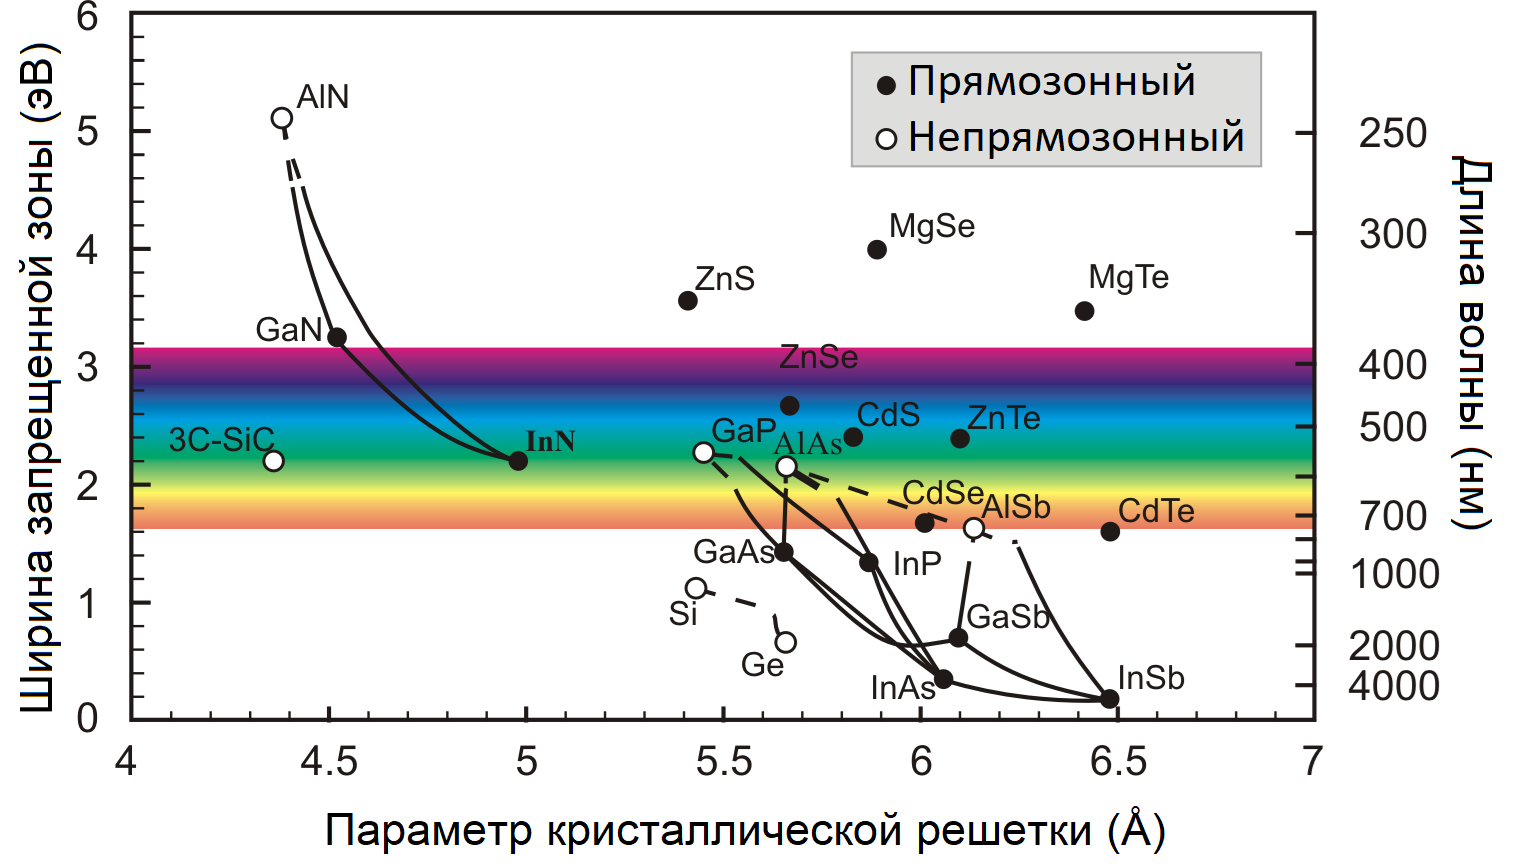
\includegraphics[width=0.9\linewidth]{Image_1}
	}
	\caption{Связь ширины запрещенной зоны некоторых полупроводников и параметра кристаллической решётки при 300~\si{\kelvin}}\label{fig:Image_1}
\end{figure}

Прямозонные A\textsuperscript{III}B\textsuperscript{V} материалы на Si~--- одна из таких проблемных, но перспективных комбинаций. Развитие технологий производства полупроводниковых приборов на основе кремния привело к  доминации этого материала в интегральной электронике и фотовольтаике. При этом он малопригоден для создания светоизлучающих приборов из-за непрямой зонной структуры и низкой вероятности излучательных переходов. Развитие технологий монолитной интеграции оптоэлектронных элементов на Si может снизить стоимость производства светоизлучающих приборов (за счет отказа от дорогостоящих A\textsuperscript{III}B\textsuperscript{V} подложек) и заменить электронные компоненты интегральных схем на оптические (для снижения энергопотребления и изоляции их компонентов друг от друга).

Монолитная интеграция тонкопленочных структур A\textsuperscript{III}B\textsuperscript{V} на Si связана с проблемами несоответствия параметров кристаллических решёток и различием их симметрии: зарождение A\textsuperscript{III}B\textsuperscript{V} на Si возможно с различной полярностью, что может приводить к образованию антифазных областей. Их границы~--- эффективные центры безызлучательной рекомбинации \cite{Takagi1998}. Образование антифазных областей возможно при росте материалов с симметрией решётки ниже, чем у подложки. Например, при формировании соединения с двумя различными атомами в примитивной решётке на поверхности одноэлементного материала (арсенид галлия (GaAs) на подложке германия (Ge) или фосфид галлия (GaP) на подложке Si). В случае сингулярной подложки антифазные области образуются при некогерентном зарождении в плоскости подложки начиная с разных типов атомов. В случае вицинальной поверхности (когда нормаль к поверхности подложки не совпадает с основным кристаллографическим направлением на малый угол, что ведет к образованию ступенчатой поверхности с террасами основной кристаллографической поверхности) и когерентном зарождении антифазные границы образуются на ступенях из нечетного количества атомов (см.~рис.~\cref{fig:Image_2}). В случае когерентного зарождения и ступеней из четного количества атомов антифазные домены не образуются \cite{Faucher2016}.

\begin{figure}[ht]
	\centerfloat{
		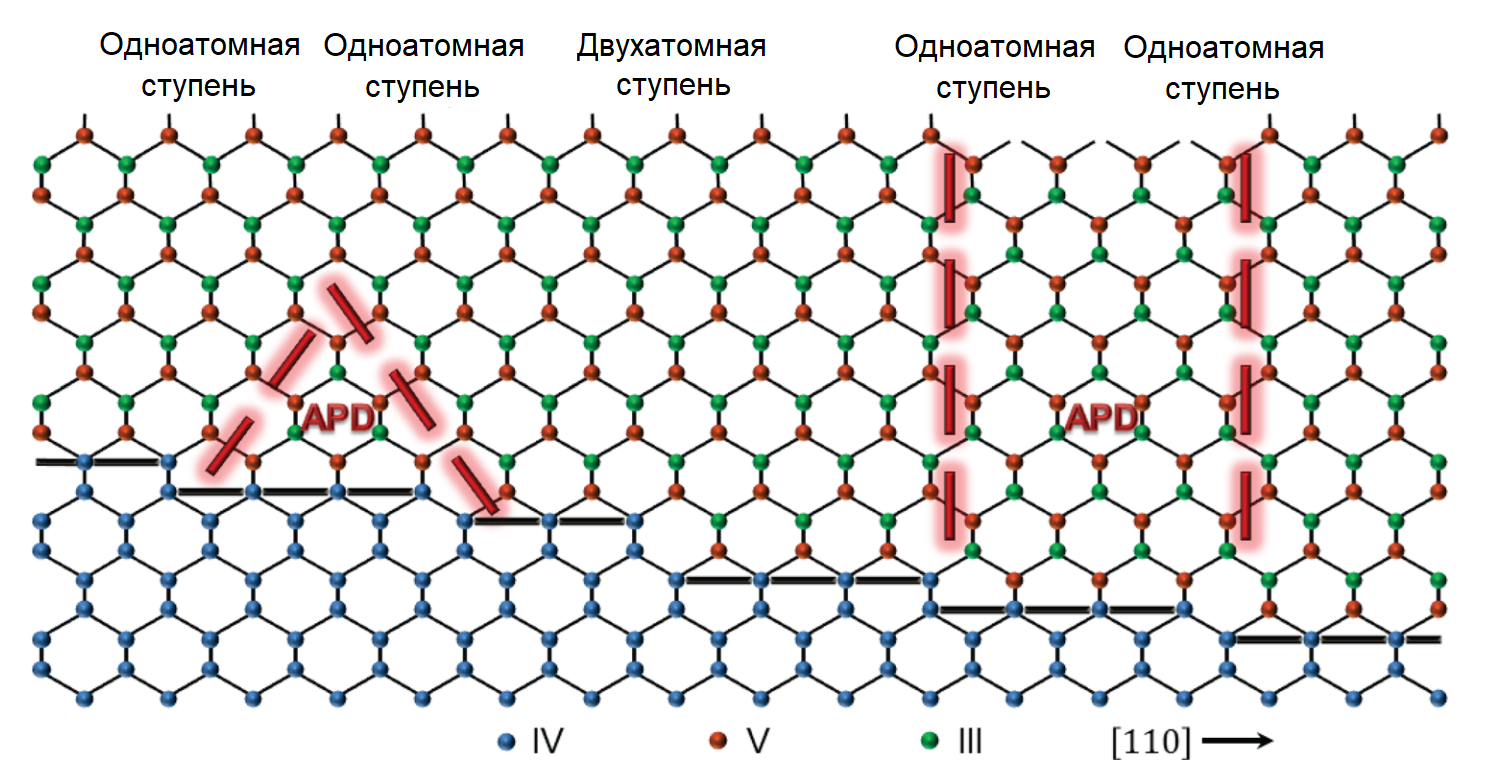
\includegraphics[width=0.9\linewidth]{Image_2}
	}
	\caption{Схема образования и аннигиляции антифазных доменов на вицинальной поверхности (001) с моно- и двухатомными ступенями}\label{fig:Image_2}
\end{figure}

Продолжающееся исследования эпитаксиального роста A\textsuperscript{III}B\textsuperscript{V} слоев на Si (в большей степени это касается твердых растворов на основе GaP) стимулирует развитие технологий синтеза функциональных слоев высокого кристаллического качества. Однако, оно ещё не позволяет достичь достаточно высокого квантового выхода излучения для их приборного применения.

Альтернативный подход формирования оптоэлектронных элементов на Si включает синтез A\textsuperscript{III}B\textsuperscript{V} эпитаксиальных наноструктур. К ним относят квантовые точки, наноостровки, нитевидные нанокристаллы (ННК) и многообразие гибридных гетероструктур \cite{Tan2018}.

В отличие от послойных гетероструктур, они имеют малую площадь интерфейса с подложкой и высокое отношение поверхности к объему \cite{Bolshakov2013, Tchernycheva2007}. Это обеспечивает эффективную релаксацию напряжений и низкую концентрацию структурных дефектов даже в системах с высоким рассогласованием кристаллических решёток \cite{Samsonenko2011}.

Более того, наноструктуры предоставляют дополнительные возможности для зонного проектирования~--- в них удается стабилизировать кристаллическую структуру, невозможную в объемном материале при нормальных условиях \cite{Mohseni2009}. Материалы с высокой степенью ионности связи, такие как нитриды, обычно имеют гексагональную кристаллическую структуру вюрцита (wurtzite, WZ), а материалы с низкой ионностью, такие как GaP и GaAs,~--- кубическую структуру сфалерита (zinc-blende, ZB). Однако, при высоком отношении поверхности к объему, в ряде случаев удается изменять стабильную структуру растущего материала, что расширяет функциональные возможности гетероструктур \cite{Spirkoska2009}. Например, GaP с кубической структурой ZB~--- непрямозонный полупроводник, а с гексагональной структурой WZ~--- прямозонный полупроводник с шириной запрещенной зоны 2,18--2,25~\si{\electronvolt}, а значит может найти применение в производстве жёлто-зеленых светодиодов \cite{Assali2013}. Вместе с тем, из-за симметрии структуре WZ не свойственно двойникование по плоскостям \{111\}, характерное для структуры ZB, что обеспечивает более высокое кристаллическое совершенство наноструктуры.

Возможность управлять формой наночастиц и их размером в диапазоне от микрометров до единиц нанометров позволяет формировать структуры с оптическим или электронным ограничением, что находит применение в оптоэлектронных приборах. Квантовые точки~--- пример успешного внедрения в промышленность наноструктур с электронным ограничением. Размер квантовых точек влияет на расстояние между энергетическими уровнями, а, следовательно, и на спектр люминесценции. Данный эффект позволяет создавать люминофоры разных цветов из одного и того же материала. При этом спектр фотолюминесценции имеет узкий и симметричный пик, а высокое кристаллическое качество обеспечивает высокую квантовую эффективность.

Для миниатюризации генераторов лазерного излучения требуется уменьшение оптически активной области резонатора. В множестве работ демонстрируется, что в ННК может формироваться резонансная стоячая оптическая волна вдоль оси ННК, с отражением от верхней и нижней граней. Широкий спектральный диапазон генерации лазерного излучения с оптической и электрической накачкой продемонстрирован на ННК из ZnO, InGaN, CdSSe, GaAs, InGaAs, AlGaAs, ZnS, CdSe, GaSb, InP и других материалов \cite{Eaton2016}.

Размер лазеров ограничен дифракционным пределом, который составляет приблизительно половину длины оптической волны в среде. Уменьшение диаметра ННК приводит к слабой оптической локализации и снижению добротности резонатора. Данное ограничение можно обойти, используя ННК в качестве платформы для лазеров на основе поверхностных плазмон-поляритонов~--- квазичастиц связанного состояния электромагнитного поля и колебаний электронной плазмы (см.~рис.~\cref{fig:Image_3}). Коллективные колебания электронов на поверхности металла имеют значительно меньшую длину волны, чем электромагнитные волны той же энергии, что позволяет уменьшить размер активной области лазера \cite{Oulton2009}.

\begin{figure}[ht]
	\centerfloat{
		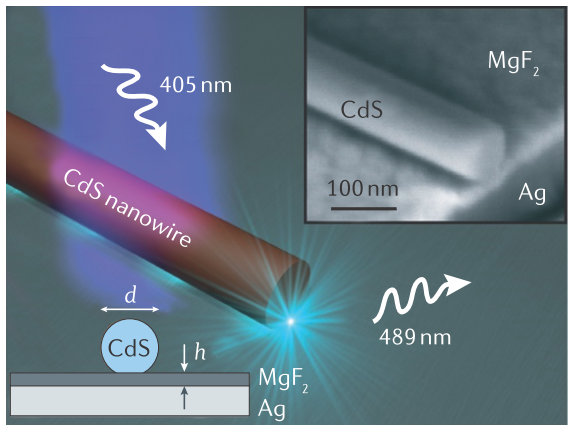
\includegraphics[width=0.6\linewidth]{Image_3}
	}
	\caption{Изображение ННК CdS на серебряной подложке, образующие резонатор лазера на основе поверхностных плазмон-поляритонов при оптическом возбуждении \cite{Oulton2009}}\label{fig:Image_3}
\end{figure}

В общем случае форма, размер и поверхностная плотность наноструктур влияет на их взаимодействие со светом и определяет эффективность вывода или захвата излучения. Этот эффект находит применение в просветляющих покрытиях солнечных элементов \cite{Mozharov2015b, Krogman2005} и определяет диаграмму направленности светоизлучающих приборов на основе массивов наногетероструктур \cite{Eaton2016}.

Несмотря на достигнутые результаты, остаются не до конца изучены закономерности формирования самоорганизованных наноструктур, устанавливающие взаимосвязь морфологии, кристаллической структуры и оптических свойств с ростовыми условиями и предварительной подготовкой подложки. Изучение данных закономерностей позволит развить методы синтеза самоорганизованных наноструктур для применения в приборах оптоэлектроники.

\section{Механизмы формирования эпитаксиальных наноструктур на кремнии}\label{sec:ch1/sec2}

\subsection{Подготовка кремниевых подложек к росту}\label{subsec:ch1/sec2/sub1}

В результате изготовления, транспортировки и хранения на поверхности Si подложек остаются загрязнения, а естественный поверхностный оксида имеет неоднородную толщину и требует высоких температур отжига для сгона. Для воспроизводимости эксперимента поверхность Si подложки должна быть чистой и атомарно гладкой, поверхностный оксид иметь контролируемую толщину. Поэтому для синтеза полупроводниковых структур требуется специальная подготовка Si подложек перед ростом.

В данной работе использовался один из распространенных методов подготовки~--- метод Шираки \cite{Ishizaka2019}. Он подразумевает кипячения в органических растворителях и аммиачно-перекисном растворе (для очистки от загрязнений), несколько циклов попеременной обработки в азотной (для окисления поверхности) и плавиковой кислотах (для травления поверхностного оксида), завершая формированием единиц монослоев нестехиометрического поверхностного оксида в перекисно-кислотном растворе, аммиачно-перекисном растворе или азотной кислоте. Подготовленные подложки сразу же загружают в эпитаксиальную установку.

Сформированный поверхностный оксид защищает поверхность Si от загрязнения и, как правило, подлежит удалению отжигом в эпитаксиальной установке, но в некоторых случаях оксид может играть роль модификатора ростовой поверхности, так как влияет на поверхностную энергию и смачиваемость поверхности металлом III группы. Металлический Ga при нанесении на поверхность оксида формируется в виде массива капель, которые протравливают тонкий слой оксида в местах поверхностных дефектов. Такие капли могут служить катализатором для самокаталитического роста ННК GaAs и GaP по механизму пар\,--\,жидкость\,--\,кристалл (ПЖК).

\subsection{Механизм роста пар\,--\,жидкость\,--\,кристалл (ПЖК)}\label{subsec:ch1/sec2/sub2}

Впервые механизм ПЖК описан Вагнером и Эллисом в 1964 году на примере роста Si ННК на подложке Si(111) методом газофазной эпитаксии (см.~рис.~\cref{fig:Image_4}) \cite{Wagner1964}. Авторы напыляли на подложку тонкий слой золота (Au), который отжигали при 950~\si{\degreeCelsius} в реакторе. При этом Si из подложки смешивался с Au с образованием жидких капель Au:Si. Сплав Au:Si с атомной долей Si 18,6\,\% имеет точку эвтектики при 363~\si{\degreeCelsius}, поэтому может быть жидким при температурах значительно ниже точки плавления компонентов (Si: 1414~\si{\degreeCelsius}, Au: 1064~\si{\degreeCelsius}).

\begin{figure}[ht]
	\centerfloat{
		\subcaptionbox{\label{fig:Image_4_1}}{%
			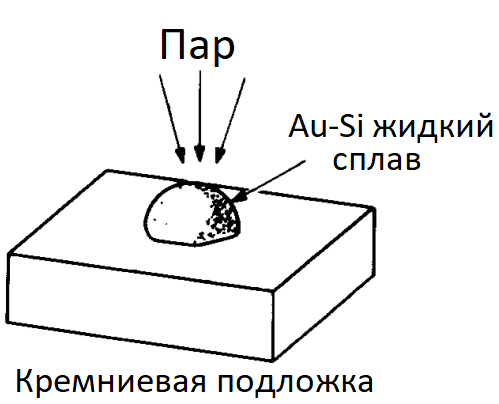
\includegraphics[width=0.3\linewidth]{Image_4_1}}
		\subcaptionbox{\label{fig:Image_4_2}}{%
			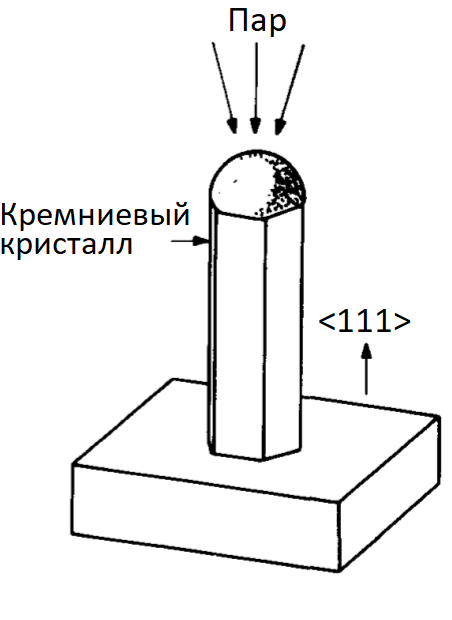
\includegraphics[width=0.3\linewidth]{Image_4_2}}
	}
	\legend{Начальные условия: жидкая Au капля катализатора на подложке~(а), рост ННК с каплей катализатора на вершине~(б)}
	\caption{Схема синтеза Si ННК по механизму ПЖК \cite{Wagner1964}}\label{fig:Image_4}
\end{figure}

Под воздействием газообразного SiCl\textsubscript{4} капля Au перенасыщается атомами Si. Реакция разложения при низкой температуре катализируется Au каплей, поэтому её называют катализатором. Эта терминология сохраняется и в случае молекулярно-пучковой эпитаксии (МПЭ), когда не происходит химического катализа, а компоненты поставляются на подложку в виде одноэлементных молекул. В таком случае капля выполняет роль резервуара материала, в котором скорость конденсация выше, чем скорость образования и роста зародышей по механизму пар\,--\,кристалл.

Поддерживаемое перенасыщение в капле вызывает непрерывное осаждение Si на границе жидкость\,--\,кристалл, что приводит к удлинению ННК. Диаметр ННК определяется размером капли.

Au также используют для роста A\textsuperscript{III}B\textsuperscript{V} ННК, однако оно легко диффундирует внутрь ННК с образованием локализованных энергетических уровней, что приводит к деградации времён жизни носителей заряда \cite{Breuer2011}. Чтобы избежать включений инородного материала существует альтернативный вариант~--- использовать в качестве катализатора собственный металл III группы. В таком случае в капле катализатора III группы  с перенасыщением растворяются только элементы V группы \cite{Breuer2011, Bolshakov2017}, что ограничивает возможность независимого управления осевой и радиальной скоростью роста \cite{Dubrovskii2015, Dubrovskii2012a}. Зародышеобразование и морфология самокаталитических ННК очень чувствительны к отношению потоков V/III: капля не образуются, если оно слишком велико, а вместо этого растут островки по механизму пар\,--\,кристалл. В обратной ситуации в капле накапливается металл III группы с её закономерным увеличением.

Рост ННК под каплей происходит послойно, на что указывают ростовые эксперименты на установках, совмещенных с просвечивающим электронным микроскопом (ПЭМ) \cite{Hofmann2008, Wen2009, Jacobsson2016}. При смене подаваемого материала с сохранением капли могут формироваться аксиальные гетероструктуры. Параллельно осевому росту идут процессы без участия капли по механизму пар\,--\,кристалл: радиальной рост ННК и формирование массива паразитных островков. В случае полного потребления капли катализатора механизм пар\,--\,кристалл становится доминирующим, что позволяет формировать гетероструктуры типа ядро\,--\,оболочка.

\subsection{Кристаллическая структура и политипизм соединений A\textsuperscript{III}B\textsuperscript{V}}\label{subsec:ch1/sec2/sub3}

Политипизм~--- разновидность полиморфизма, при которой в разных кристаллических модификациях элемента или химического соединения можно выделить периодичные в двух направлениях слои с идентичным (или почти идентичным) строением. Обладающие политипизмом вещества называются политипами. Для существования политипов необходимо, чтобы принципиально одинаковый способ наложения слоёв (смещение, вращение) мог дать как минимум два неэквивалентных расположения второго слоя относительно первого. В плоскости плотноупакованного слоя политипы имеют одинаковый параметр решётки, в перпендикулярном направлении периоды различны и кратны расстоянию между соседними осями.

Система Л.\,С.~Рамсделла наиболее компактна для обозначения политипов, хотя и неоднозначна для политипов с одинаковым числом слоёв в элементарной ячейке при разных последовательностях укладки. В ней цифрой указывается число слоёв в одной элементарной ячейке, а буквой C, H, R или T обозначается симметрия решётки (C~--- кубическая, H~--- гексагональная, R~--- ромбоэдрическая и T~--- тригональная). Соединения A\textsuperscript{III}B\textsuperscript{V} образуют два политипа: ZB~(3C) и WZ~(2H) (см.~рис.~\cref{fig:Image_5}).

\begin{figure}[ht]
	\centerfloat{
		\hfill
		\subcaptionbox{\label{fig:Image_5_1}}{%
			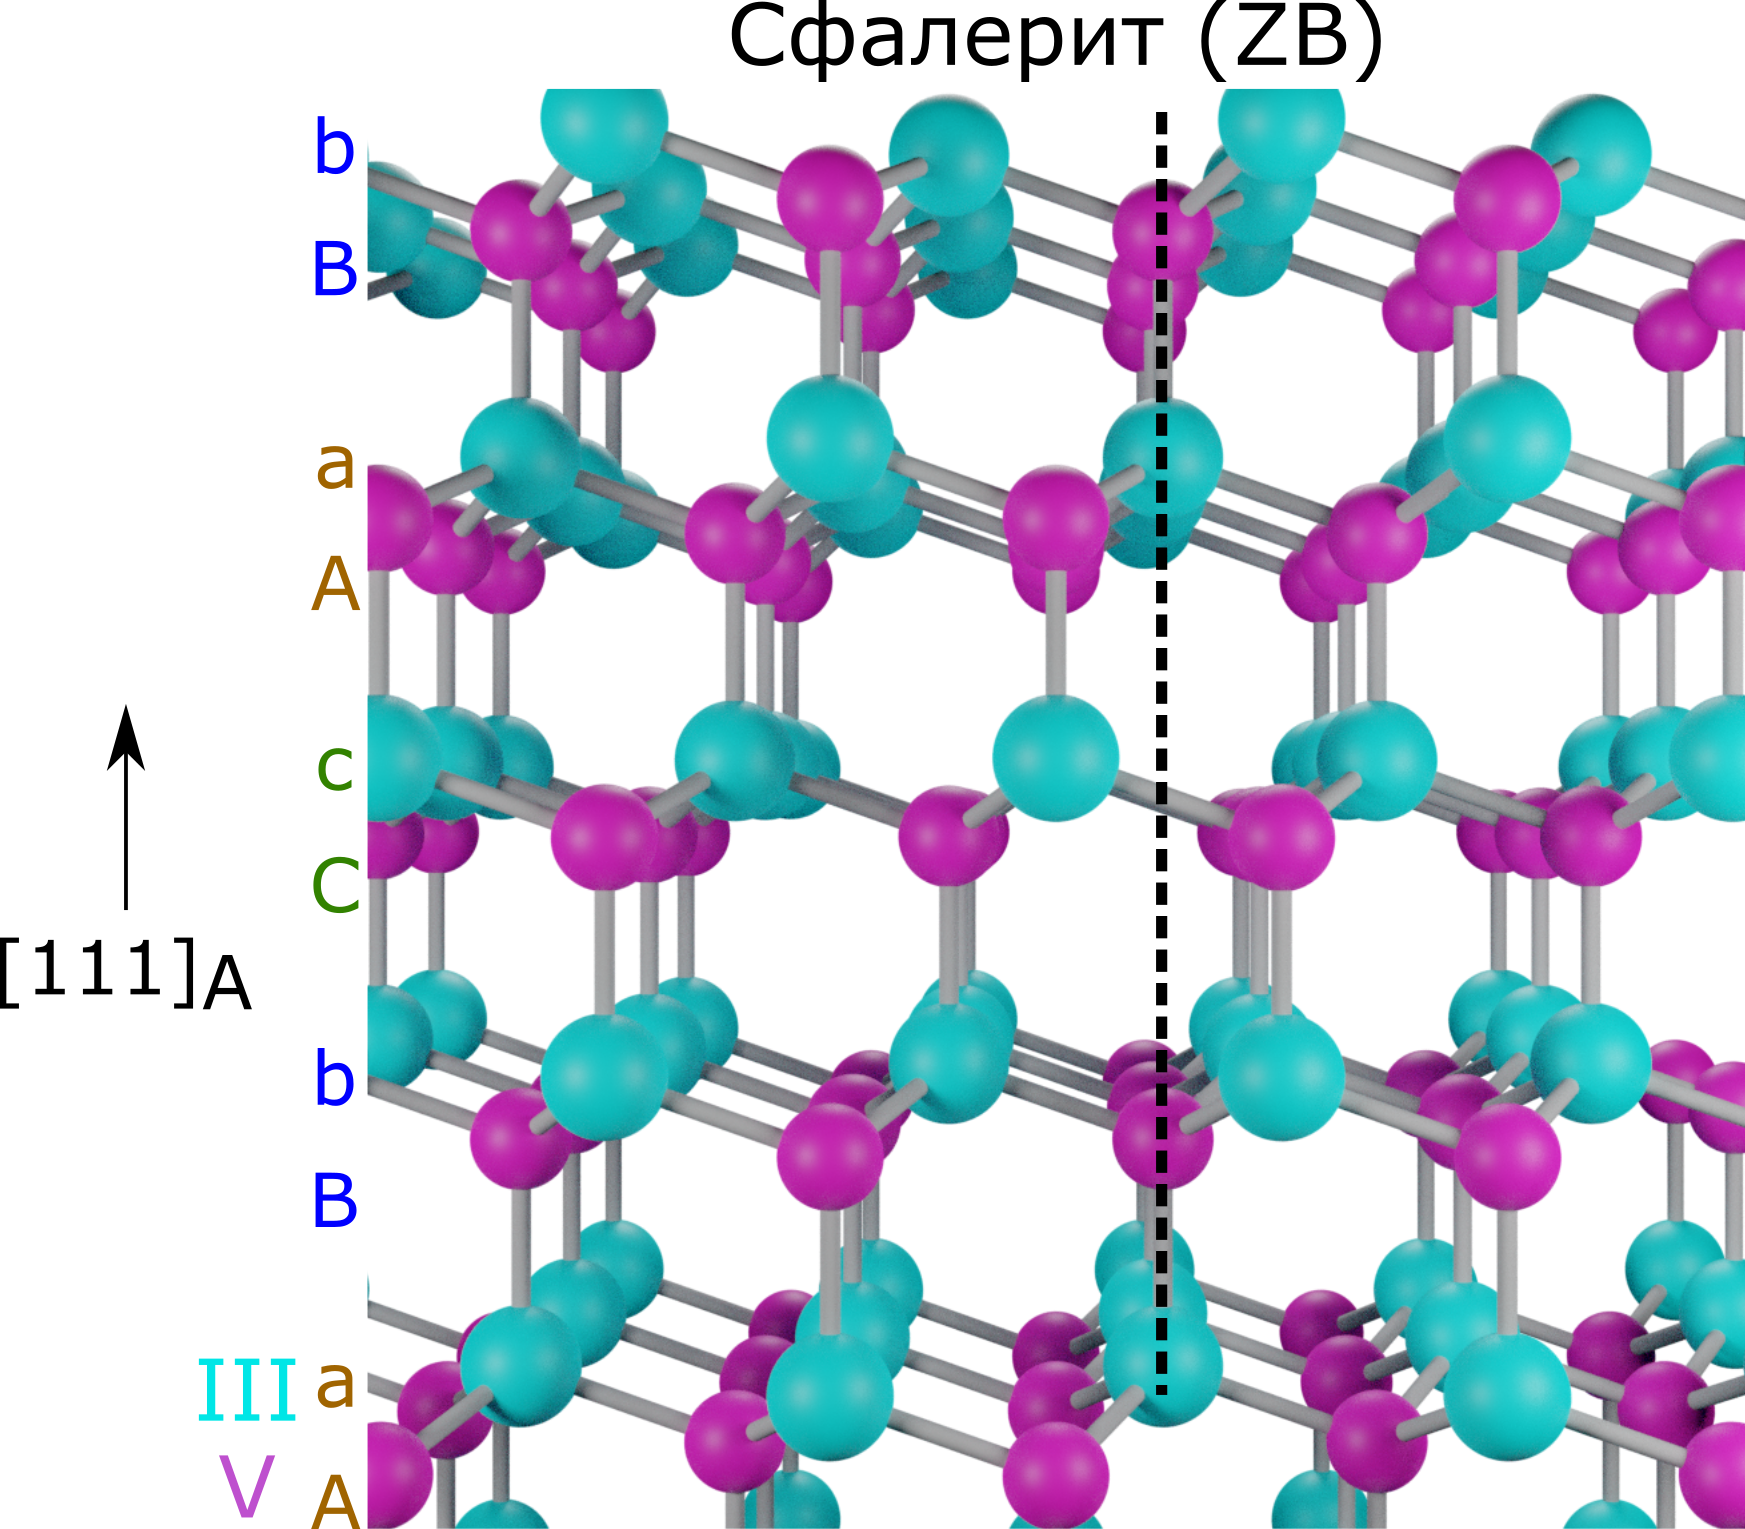
\includegraphics[width=0.3\linewidth]{Image_5_1}}
		\hfill
		\subcaptionbox{\label{fig:Image_5_2}}{%
			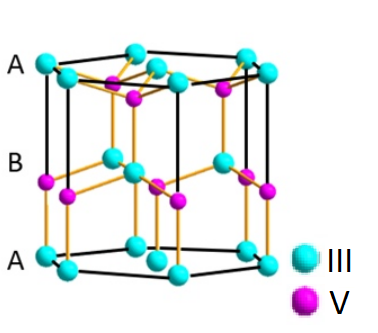
\includegraphics[width=0.35\linewidth]{Image_5_2}}
		\hfill
	}
	\caption{Кристаллическая структура ZB\,(3C)~(а) и WZ\,(2H)~(б)}\label{fig:Image_5}
\end{figure}

Кристаллическая структура ZB схожа с кристаллической структурой Si (структурой алмаза), которую можно представить как две кубических гранецентрированных решётки, смещенных друг относительно друга по главной диагонали куба на четверть её длины.

В случае решёток типа ZB\,(3C) и WZ\,(2H) поверхности (111) и \((\overline{1}\overline{1}\overline{1})\) неэквивалентны (в случае WZ говорят о плоскостях (0001) и \((000\overline{1})\)). Структуру ZB\,(3C) можно представить в виде каркаса тетраэдров AB\textsubscript{4} или BA\textsubscript{4}. Все тетраэдры ориентированны одинаково, что фактически приводит к симметрии тетраэдра, а не куба. Каждая вершина тетраэдра общая для трех соседних тетраэдров. Направление связи между ближайшими атомами А (группы III) и В (группы V) в кристаллической решётке ZB обозначается <111>. В структуре алмаза, в элементарной ячейке которой атомы только одного элемента, эти тетраэдры эквивалентны между собой. На поверхности (111) атом А связан с тремя атомами В нижележащего монослоя или атом B связан с одним атомом A нижележащего монослоя. На поверхности \((\overline{1}\overline{1}\overline{1})\) ситуация обратная: атом B связан с тремя атомами A нижележащего монослоя или атом A связан с одним атомом B нижележащего монослоя. Плоскость (111) называют А-полярной, а противоположную ей~--- В-полярной. A- и B-полярные плоскости также обозначают (111)A и (111)B соответственно.

Можно определить поверхность (111)A, как оканчивающуюся элементами III группы, а поверхность (111)B, как оканчивающуюся элементами V группы, однако в условиях эпитаксиального роста терминация поверхности определяется ростовыми условиями.

Подобным же образом структуру WZ\,(2H) можно представить в виде каркаса тетраэдров AB\textsubscript{4} или BA\textsubscript{4}. Структура WZ отличаются от ZB лишь взаимной ориентацией тетраэдров. Периодичность вдоль направления <111> типа ABCABC\dots, где каждая из букв A, B и C обозначает латеральную ориентацию слоя толщиной в два атома, состоящего из одного слоя с атомами группой III и одного слоя с атомами группы V, соответствует структуре ZB (см.~рис.~\cref{fig:Image_5}). Периодичность вдоль направления <0001> типа ABAB\dots соответствует структуре WZ \cite{Kriegner2011}. Аналогично плоскости (0001) и \((000\overline{1})\) обозначают как (0001)A и (0001)B.

\subsection{Эпитаксиальная ориентация A\textsuperscript{III}B\textsuperscript{V} наноструктур на Si}\label{subsec:ch1/sec2/sub4}

Эпитаксиальная ориентация наноструктур может быть наглядно продемонстрирована на примере ННК. Как правило, наноструктуры растут вдоль кристаллографического направления, которое минимизирует полную свободную энергию \cite{Wagner1964}. Полная свободная энергия равна сумме объемного вклада, энергии границ раздела катализатор\,--\,пар, катализатор\,--\,кристалл и пар\,--\,кристалл. Последние два вклада зависят от кристаллической ориентации границы раздела. При образовании первого монослоя по механизму ПЖК доминирует вклад энергией границы раздела катализатор\,--\,кристалл.

ННК преимущественно растут ортогонально поверхности с самой низкой поверхностной свободной энергией \cite{Wagner1964}. У материалов A\textsuperscript{III}B\textsuperscript{V} с кристаллической решёткой ZB самую низкую поверхностную свободную энергию имеет грань (111)B, а у материалов A\textsuperscript{III}B\textsuperscript{V} со структурой WZ~--- грань (0001) \cite{Fortuna2010}. Поэтому ННК растут преимущественно вдоль направлений <111>B и <0001> соответственно. Ориентация ННК относительно поверхности Si подложки в зависимости от её кристаллографической ориентации для двух возможных случаев ориентации ZB зародышей показана на рисунке \cref{fig:Image_6}.

\begin{figure}[ht]
	\centerfloat{
		\subcaptionbox{\label{fig:Image_6_1}}{%
			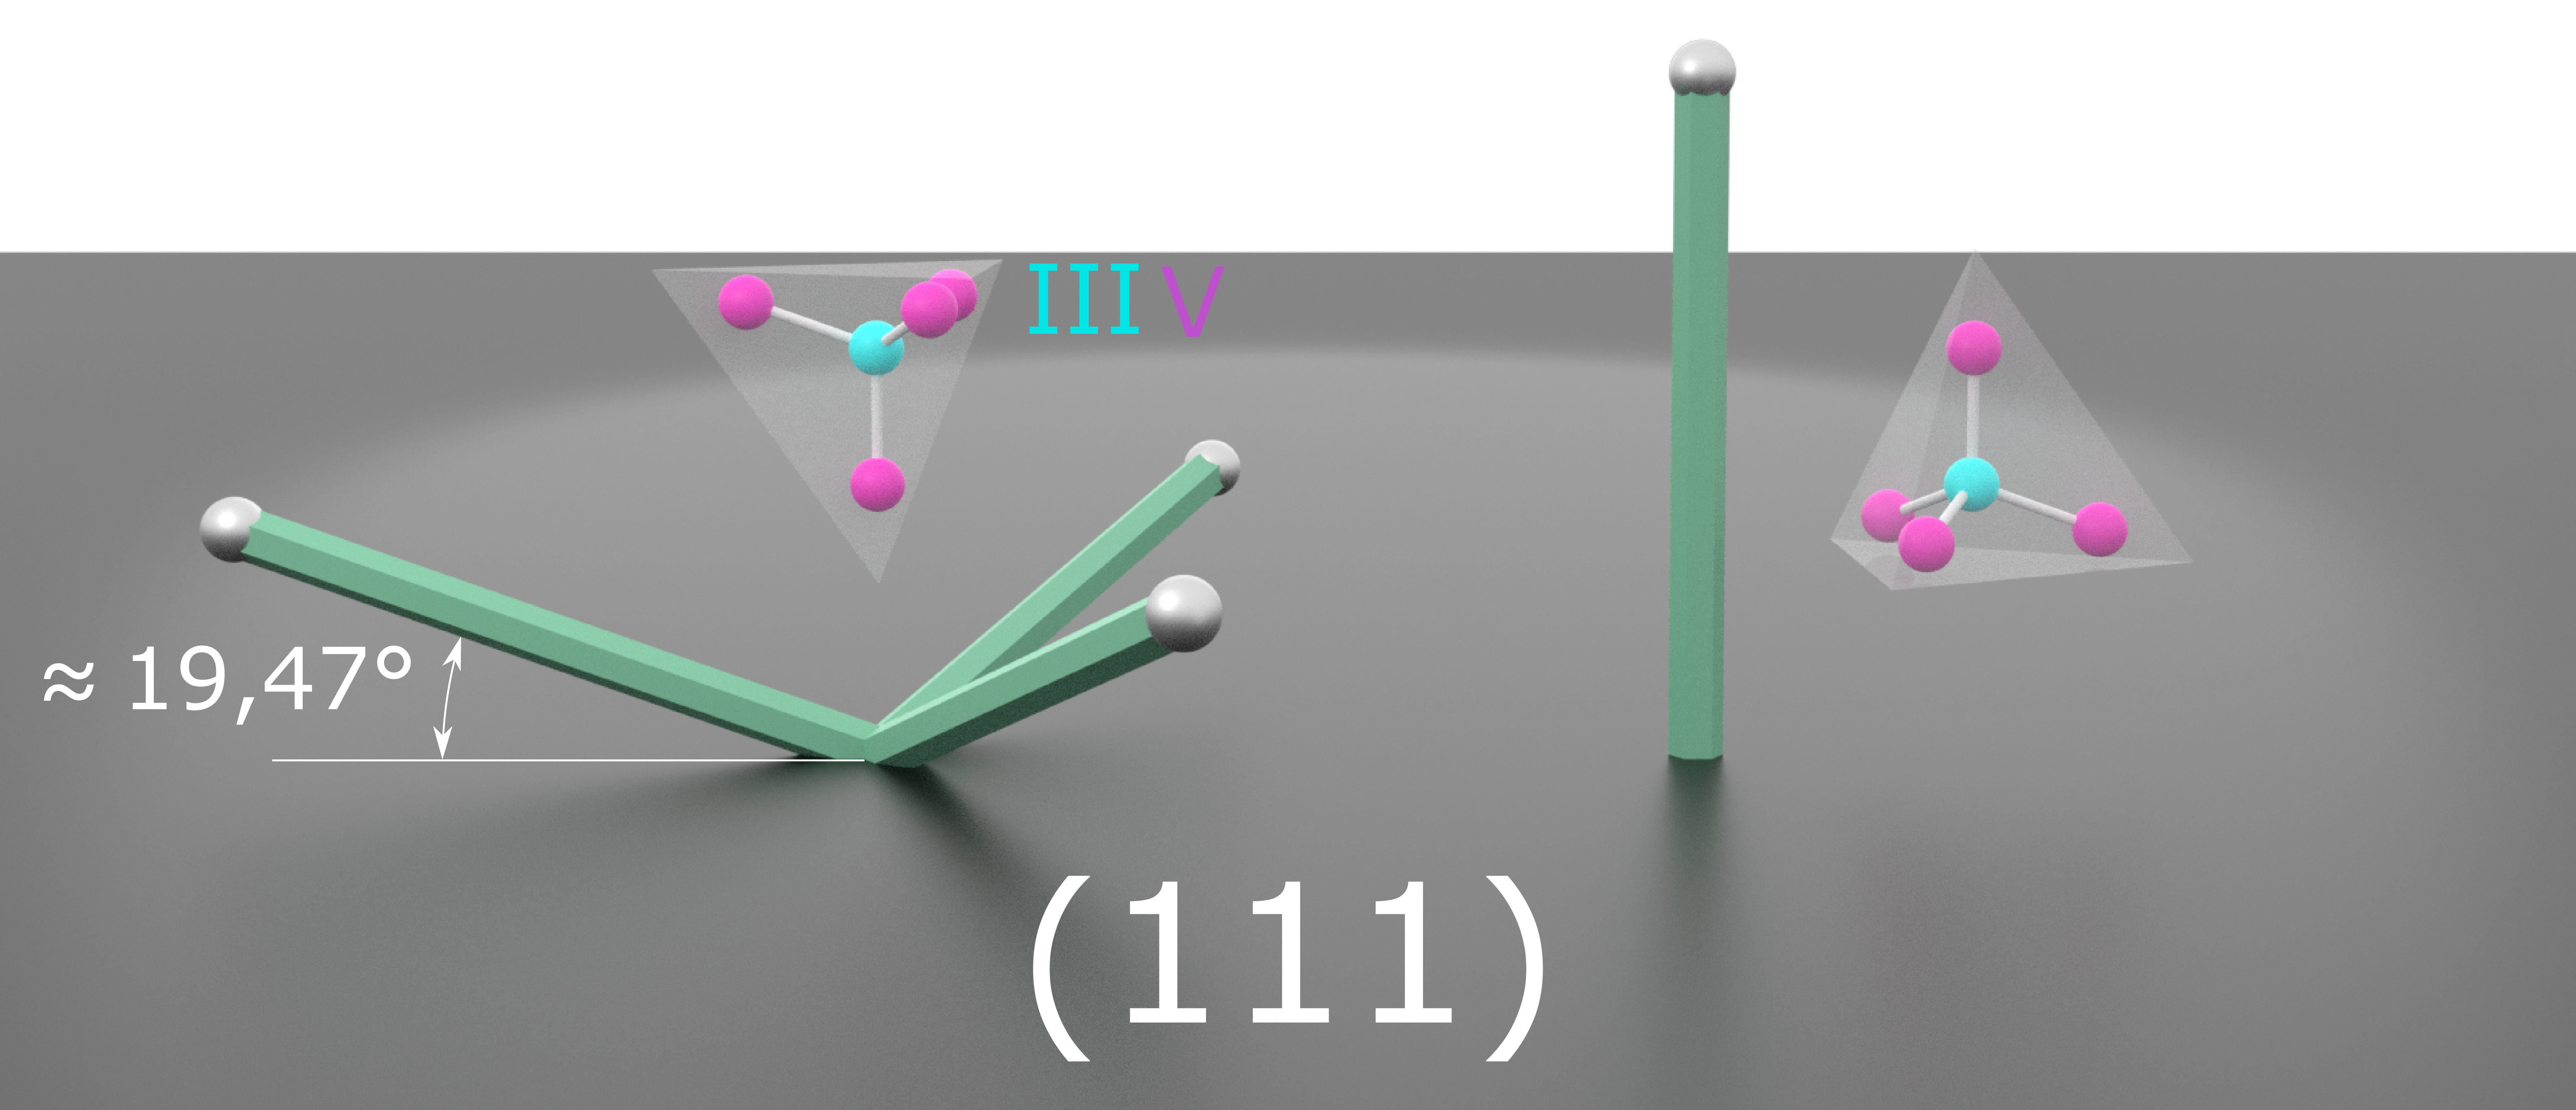
\includegraphics[width=0.9\linewidth]{Image_6_1}}

		\subcaptionbox{\label{fig:Image_6_2}}{%
			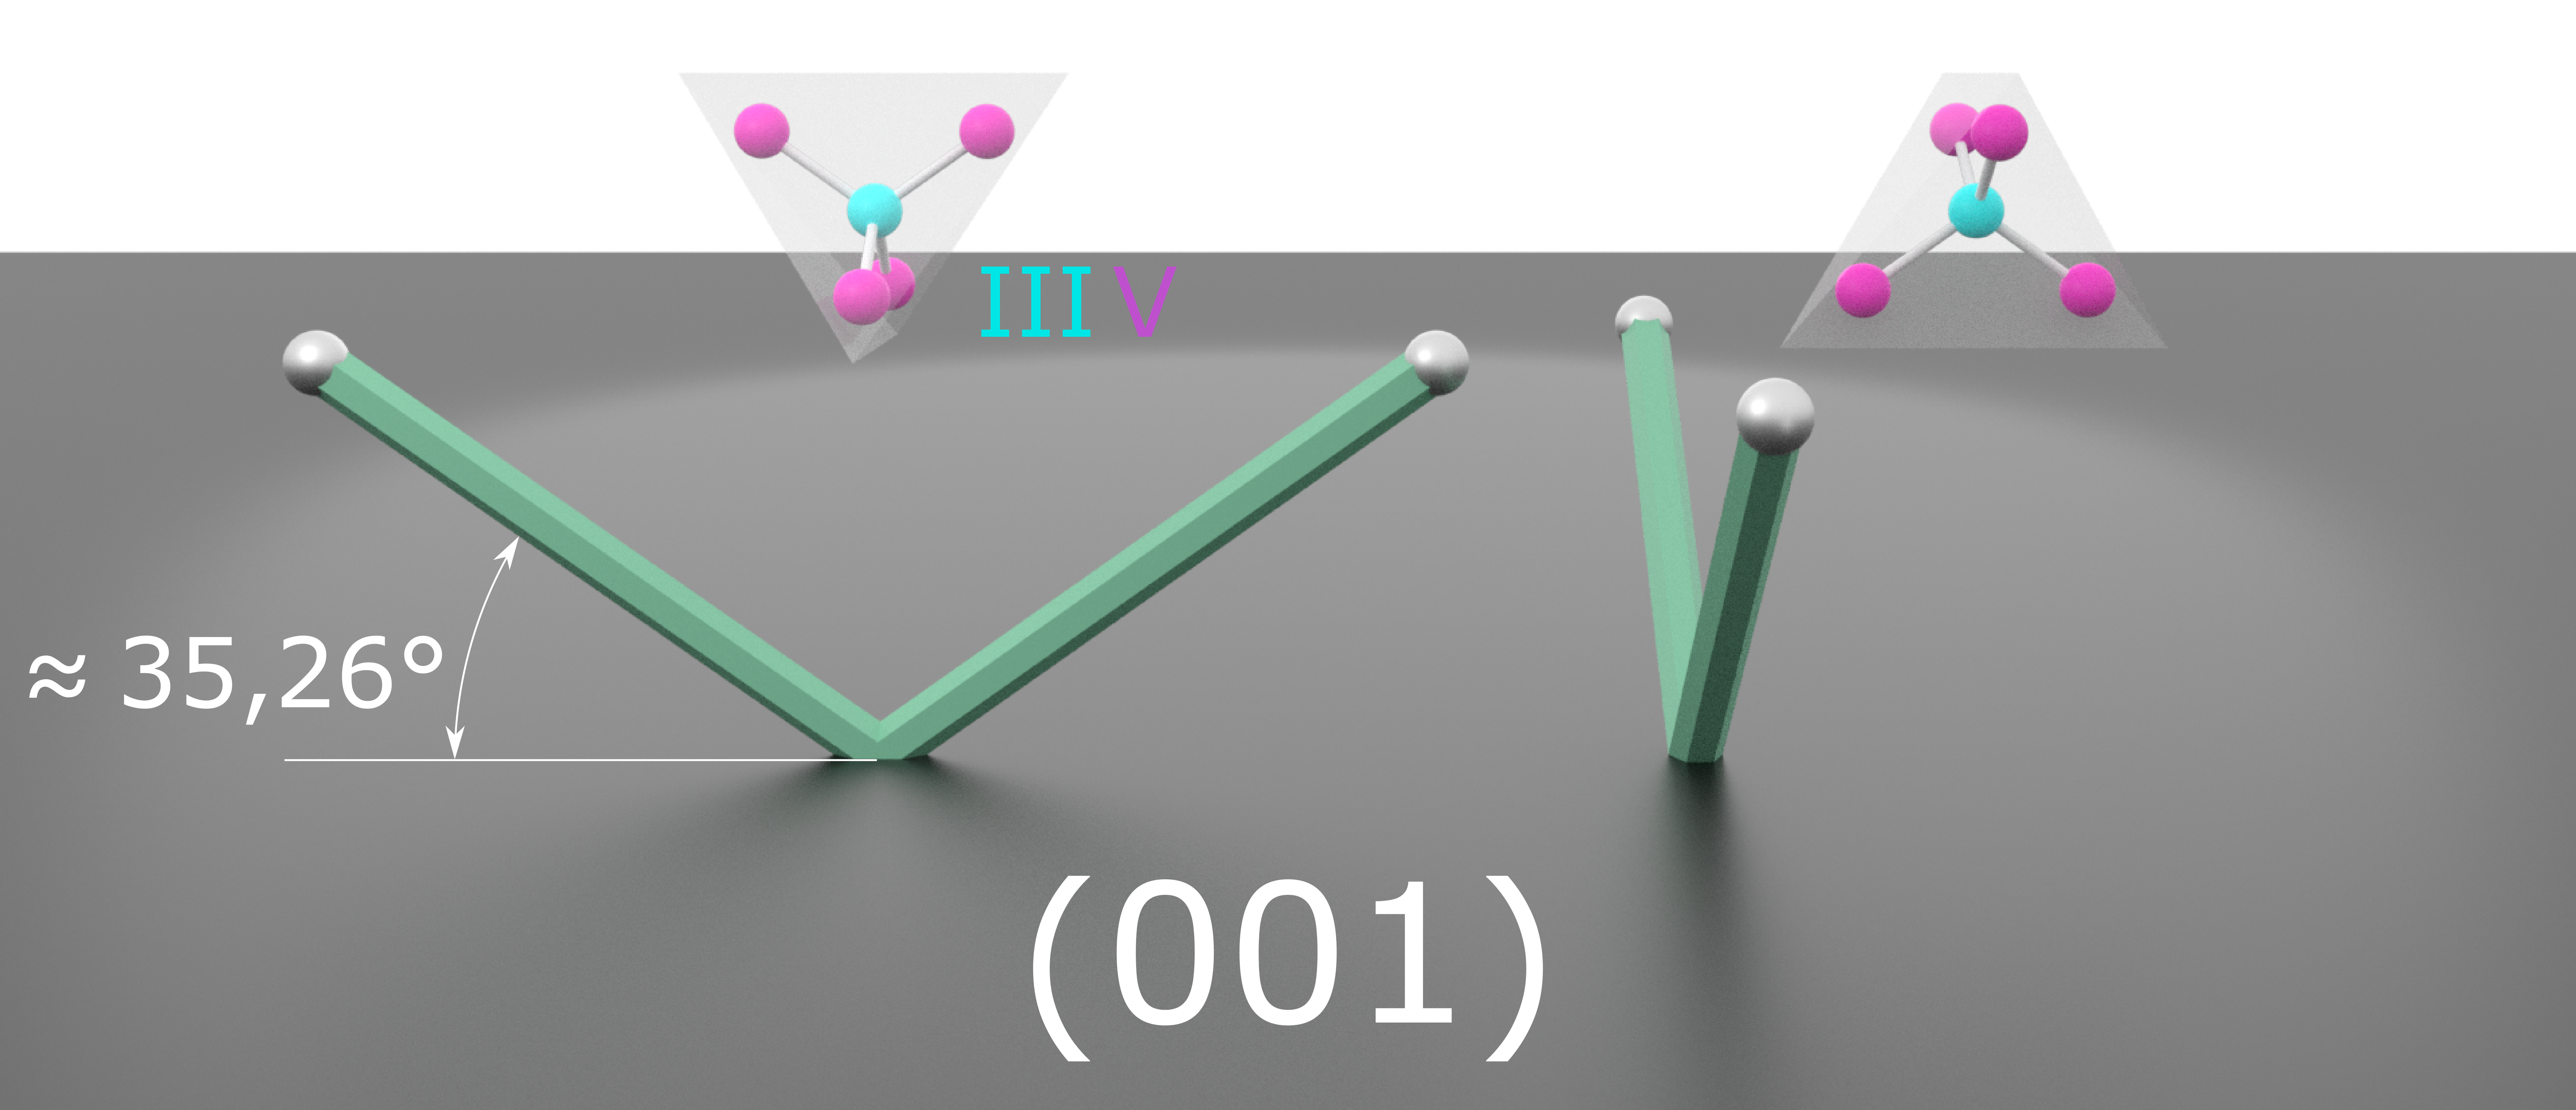
\includegraphics[width=0.44\linewidth]{Image_6_2}}
		\subcaptionbox{\label{fig:Image_6_3}}{%
			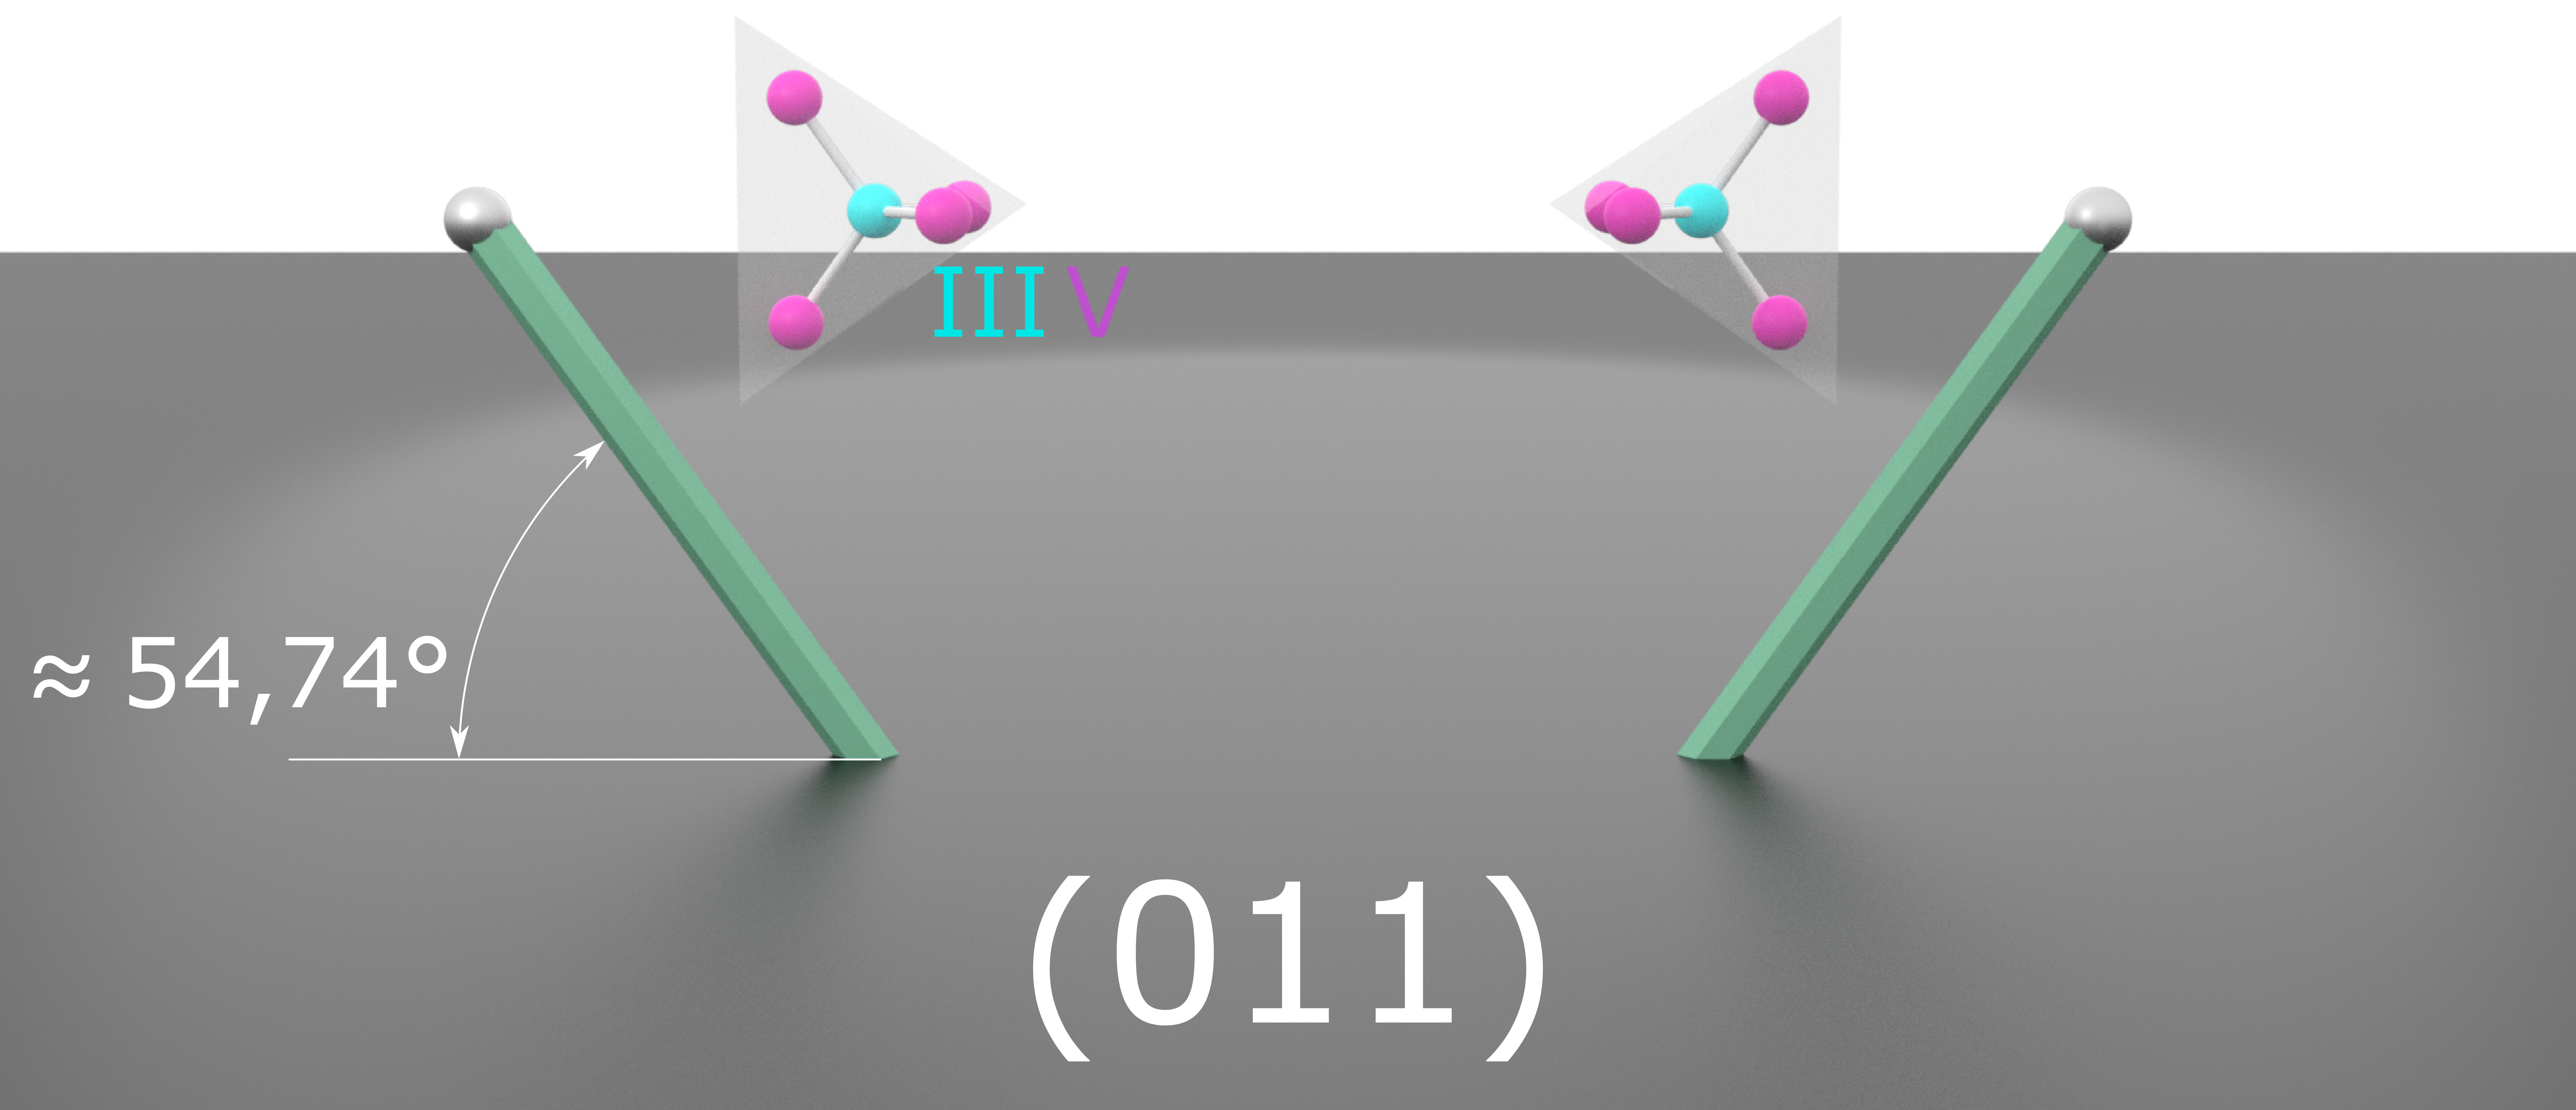
\includegraphics[width=0.44\linewidth]{Image_6_3}}
	}
	\legend{Ориентации подложек: (111)~(а), (001)~(б) и (110)~(в)}
	\caption{Схематическое изображение направлений роста <111>B и эпитаксиальных ориентаций ННК относительно поверхности подложек Si различной кристаллографической ориентации}\label{fig:Image_6}
\end{figure}

Так как A\textsuperscript{III}B\textsuperscript{V} ННК растут вдоль направления <111>B, то в случае образования на подложках Si(111) зародыша с ориентацией B~--- ННК растут вертикально, а в случае образования зародыша с ориентацией A~--- под углом к подложке в трёх эквивалентных направлениях <111>B (см.~рис.~\cref{fig:Image_6_1}). Если ZB зародыш с ориентацией A испытывает вращательное двойникование вокруг оси <111>, ортогональной поверхности подложки, то ННК растут вдоль трёх дополнительных направлений, развернутых на 180\textdegree вокруг данной оси.

\subsection{Двумерные дефекты и формирование WZ/ZB перехода в A\textsuperscript{III}B\textsuperscript{V} наночастицах}\label{subsec:ch1/sec2/sub5}

В процессе роста A\textsuperscript{III}B\textsuperscript{V} наночастиц образуются следующие типы двумерных дефектов:  для ZB структуры типичны дефекты вращательного двойникования на 180\textdegree вокруг осей <111> (начало и конец двойниковых сегментов могут рассматриваться как элементарное WZ включение), а для WZ структуры типичны дефекты упаковки AB\textbf{ABC}BC и AB\textbf{ABCA}CA вдоль направления роста <0001> (которые могут рассматриваться как элементарные ZB включения) \cite{knoll2014}.

В некоторых случаях данные дефекты приводят к стабилизации нестабильной фазы с сформированием дефектов спонтанной переброски кристаллической структуры \cite{Cirlin2010}. В работе \cite{Glas2007} проведен теоретический анализ барьеров нуклеации треугольных островков со структурой ZB и WZ в процессе роста самокаталитических A\textsuperscript{III}B\textsuperscript{V} ННК. Показано, что нуклеация островка на тройной линии (границе пар\,--\,жидкость\,--\,кристалл) более выгодна со структурой WZ, чем со структурой ZB. Критерий нуклеации на тройной линии:

\begin{equation}
	\label{eq:eq_1}
	\gamma_{lV} - \gamma_{lL} - \gamma_{LV} \sin(\beta) < 0,
\end{equation}
где \(\gamma\)~--- удельная поверхностная энергия границы кристалл\,--\,пар \((lV)\), кристалл\,--\,жидкость \((lL)\) и жидкость\,--\,пар \((LV)\), \(\beta\)~--- контактный угол капли (см.~рис.~\cref{fig:Image_7}).

\begin{figure}[ht]
	\centerfloat{
		\subcaptionbox{\label{fig:Image_7_1}}{%
			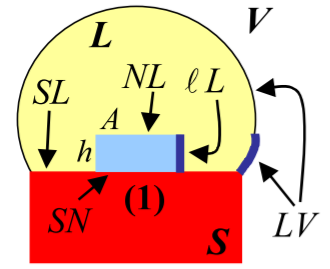
\includegraphics[width=0.3\linewidth]{Image_7_1}}
		\subcaptionbox{\label{fig:Image_7_2}}{%
			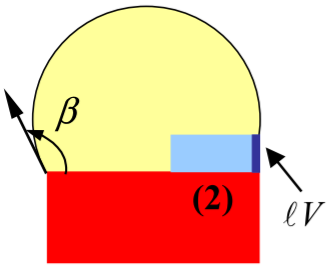
\includegraphics[width=0.3\linewidth]{Image_7_2}}
	}
	\legend{Обозначения интерфейсов: кристалл\,--\,зародыш \((SN)\), зародыш\,--\,жидкость \((NL)\), кристалл\,--\,жидкость \((SL)\), жидкость\,--\,пар \((LV)\), кристалл\,--\,жидкость \((lL)\) и жидкость\,--\,пар \((LV)\); \(\beta\)~--- контактный угол капли}
	\caption{Схема зарождения вдали от тройной линии~(а) и на тройной линии~(б) \cite{Glas2007}}\label{fig:Image_7}
\end{figure}

В ходе стационарного роста самокаталитических ННК (контактный угол капли \(\beta\approx 130\){\textdegree}) зарождение происходит вдали от тройной линии, что приводит к преимущественному формированию структуры ZB \cite{Cirlin2010}. Для ННК, капли которых израсходованы, характерно наличие в верхней части последовательность ZB\,--\,WZ\,--\,ZB \cite{Spirkoska2009, Ambrosini2011}. Это связывают с изменением контактного угла капли от \(\approx 110\){\textdegree} до 0{\textdegree} через значение 90{\textdegree}, где \(\sin(\beta)\) имеет максимум.

\subsection{Капельная эпитаксия}\label{subsec:ch1/sec2/sub6}

Капельная эпитаксия~--- метод формирования эпитаксиальных наночастиц путем кристаллизации металлических капель элемента III группы в потоке элемента V группы (см.~рис.~\cref{fig:Image_8_1}).

\begin{figure}[ht]
	\centerfloat{
		\subcaptionbox{\label{fig:Image_8_1_1}}{%
			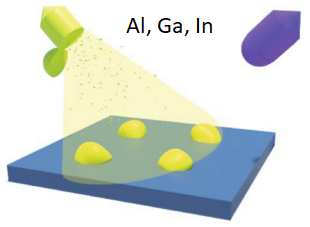
\includegraphics[width=0.3\linewidth]{Image_8_1_1}}
		\subcaptionbox{\label{fig:Image_8_1_2}}{%
			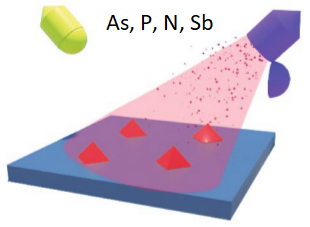
\includegraphics[width=0.3\linewidth]{Image_8_1_2}}
	}
	\caption{Схема метода капельной эпитаксии: нанесение материала III группы~(а), кристаллизации капель в потоке элементов V группы~(б) \cite{Gurioli2019}}\label{fig:Image_8_1}
\end{figure}

Нанесение менее монослоя металла на поверхность Si формирует смачивающий слой с соответствующей реконструкцией (подробнее см.~подраздел~\cref{subsec:ch2/sec1/sub2}) \cite{Park1988}. Нанесение Ga сверх монослоя формирует массив капель, плотность и размер которых зависят от диффузионной длины адатомов и количества нанесенного материала (см.~рис.~\cref{fig:Image_8_2}). После формирования капель источник металла закрывают, а капли кристаллизуют под потоком элемента V группы.

\begin{figure}[ht]
	\centerfloat{
		\subcaptionbox{\label{fig:Image_8_2_1}}{%
			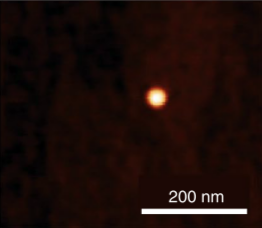
\includegraphics[width=0.3\linewidth]{Image_8_2_1}}
		\subcaptionbox{\label{fig:Image_8_2_2}}{%
			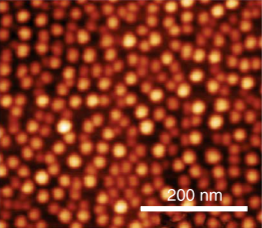
\includegraphics[width=0.3\linewidth]{Image_8_2_2}}
}
	\caption{Пример формирования частиц различной плотности при высоких~(а) и низких~(б) температурах подложки AlGaAs(001) во время осаждения металла \cite{Gurioli2019}}\label{fig:Image_8_2}
\end{figure}

Терминация поверхности элементами V группы вокруг капли может способствовать миграции адатомов металла из капли. При доминировании этого процесса образуются кольцеобразные эпитаксиальные частицы (см.~рис.~\cref{fig:Image_8_3}) \cite{Gurioli2019, mano2005}.

\begin{figure}[ht]
	\centerfloat{
		\subcaptionbox{\label{fig:Image_8_3_1}}{%
			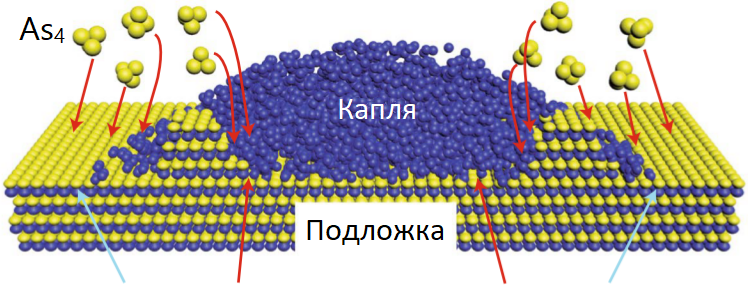
\includegraphics[width=0.65\linewidth]{Image_8_3_1}}
		
		\subcaptionbox{\label{fig:Image_8_3_2}}{%\textbf{}
			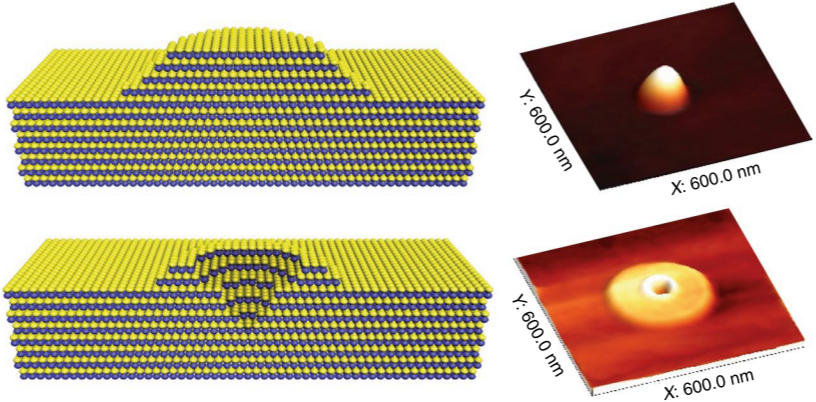
\includegraphics[width=0.65\linewidth]{Image_8_3_2}}
	}
	\caption{Схема процесса капельной эпитаксии~(а). Схема и АСМ изображения островков и кольцеобразных наноструктур, полученных методом капельной эпитаксии~(б) \cite{Gurioli2019}}\label{fig:Image_8_3}
\end{figure}

\subsection{Бескаталитический механизм роста}\label{subsec:ch1/sec2/sub7}

ННК некоторых материалов (например InAs и III-нитридов) могут быть выращены без использования капель катализатора по самоиндуцированному механизму пар\,--\,кристалл \cite{Ristic2008, Bolshakov2014}. Он основан на механизме островкового роста Вольмера\,--\,Вебера, который реализуется, когда атомы растущего материала сильнее связаны друг с другом, чем с подложкой. 

Синтез таких ННК начинается с образования WZ зародыша с ориентацией [0001] перпендикулярно ростовой поверхности даже в случае аморфной подложки \cite{Stoica2008, Corfdir2009}. Ориентация зародыша в плоскости перпендикулярной направлению роста наследуется от подложки. С увеличением объема зародыша под влиянием поверхностных энергий адсорбированные атомы (адатомы) начинают преимущественно встраиваться в плоскость (0001), что приводит к аксиальному удлинению (см.~рис.~\cref{fig:Image_9}) \cite{Dubrovskii2012b}.

\begin{figure}[ht]
	\centerfloat{
		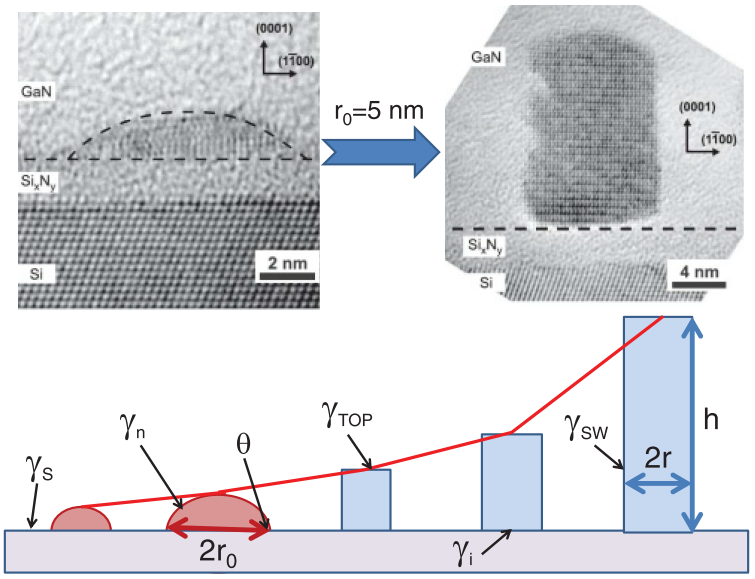
\includegraphics[width=0.7\linewidth]{Image_9}
	}
	\caption{Схема самоиндуцированного механизма роста GaN ННК \cite{Dubrovskii2012b}}\label{fig:Image_9}
\end{figure}

\FloatBarrier
           % Глава 1
\chapter{Экспериментальные методы}\label{ch:ch2}

\section{Молекулярно-пучковая эпитаксия (МПЭ)}\label{sec:ch2/sec1}

Изучаемые в данной работе наноструктуры синтезированы методом МПЭ, в основе
которого лежит взаимодействие пучков атомов или молекул с кристаллической
подложкой в условиях сверхвысокого вакуума \((\sim 10^{-10}\)~\si{\torr}). При
таких давлениях длина свободного пробега молекул намного превышает
геометрические размеры реактора. Данная технология позволяет снизить
концентрацию инородных включений в синтезированных гетероструктурах,
контролировать толщину слоев и профиль легирования на уровне атомных размеров.

Структуры синтезировались на установке МПЭ Veeco GEN III
(см.~рис.~\cref{fig:Image_10}). Установка состоит из трёх высоковакуумных
камер: загрузочной (остаточное давление \(\sim 10^{-8}\)~\si{\torr}),
промежуточной (\(\sim 10^{-10}\)~\si{\torr}) и ростовой (\(\sim
10^{-10}\)~\si{\torr}). Откачка осуществляется турбиной, крионасосом,
магниторазрядным и титановым сублимационным насосами.

\begin{figure}[ht] \centerfloat{
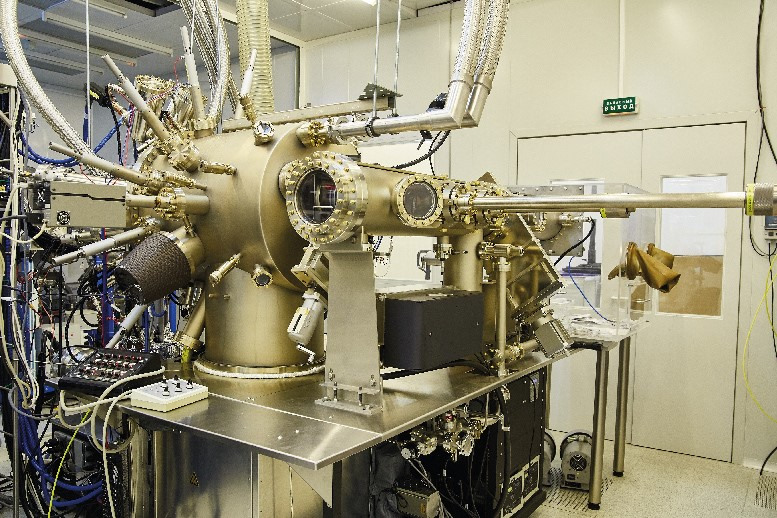
\includegraphics[width=0.6\linewidth]{Image_10} } \caption{Установка МПЭ Veeco
GEN III}\label{fig:Image_10} \end{figure}

Для поддержания высокого вакуума и предотвращения взаимного нагрева источников
ростовая камера в дополнение к насосам оснащена криопанелью~--- ёмкостью с
протекающим в ней жидким азотом. Криопанель эффективно адсорбирует частицы
остаточного газа в ростовой камере из-за низкой температуры своих стенок.

Давление в камерах контролируется ионизационными вакуумными датчиками
Байярда\,--\,Альперта, калиброванными по N\textsubscript{2}. Принцип их
действия: электроны, испускаемые накалённым катодом, ускоряются в направлении
цилиндрической сетки электрическим полем, ионизируя на пути молекулы
остаточного газа. За сеткой в центре цилиндра находится собирающий
положительные ионы коллектор. Учитывая рабочие напряжения и ток накала катода,
устанавливается зависимость между силой тока ионов в цепи коллектора и
давлением. Для контроля парциальных давлений элементов остаточного газа и
молекулярных пучков установка оснащена квадрупольным масс-спектрометром.

Перед загрузкой в ростовую камеру подложки проходят процедуру дегазации~---
удаления остаточной воды с поверхности подложек и держателей нагревом до
\(\approx 300\)~\si{\degreeCelsius}. После дегазации подложку переносят в
ростовую камеру на подложкодержатель (манипулятор), который позволяет
разворачивать подложку между трансферным и ростовым положением, вращать
подложку вокруг своей оси (для достижения однородных условий роста на всей
поверхности подложки). На манипуляторе за подложкой находится термопара и
двузонный нагревательный элемент, способный нагревать подложку до
1000~\si{\degreeCelsius}. Термопара манипулятора не касается подложки, поэтому
для уточнения температуры подложки используется пирометр.

\subsection{Молекулярные источники и измерение потока}\label{sec:ch2/sec1/sub1}

Ростовая камера МПЭ установки (см.~рис.~\cref{fig:Image_11}) оснащена
следующими молекулярными источниками:

\begin{enumerate}[beginpenalty=10000] \item эффузионными ячейками III группы
	Ga, Al, In; \item эффузионными ячейками легирующих Si и Be; \item крекерными
	источниками V группы P и As; \item плазменным источником активированного N.
	\end{enumerate}

\begin{figure}[ht] \centerfloat{ 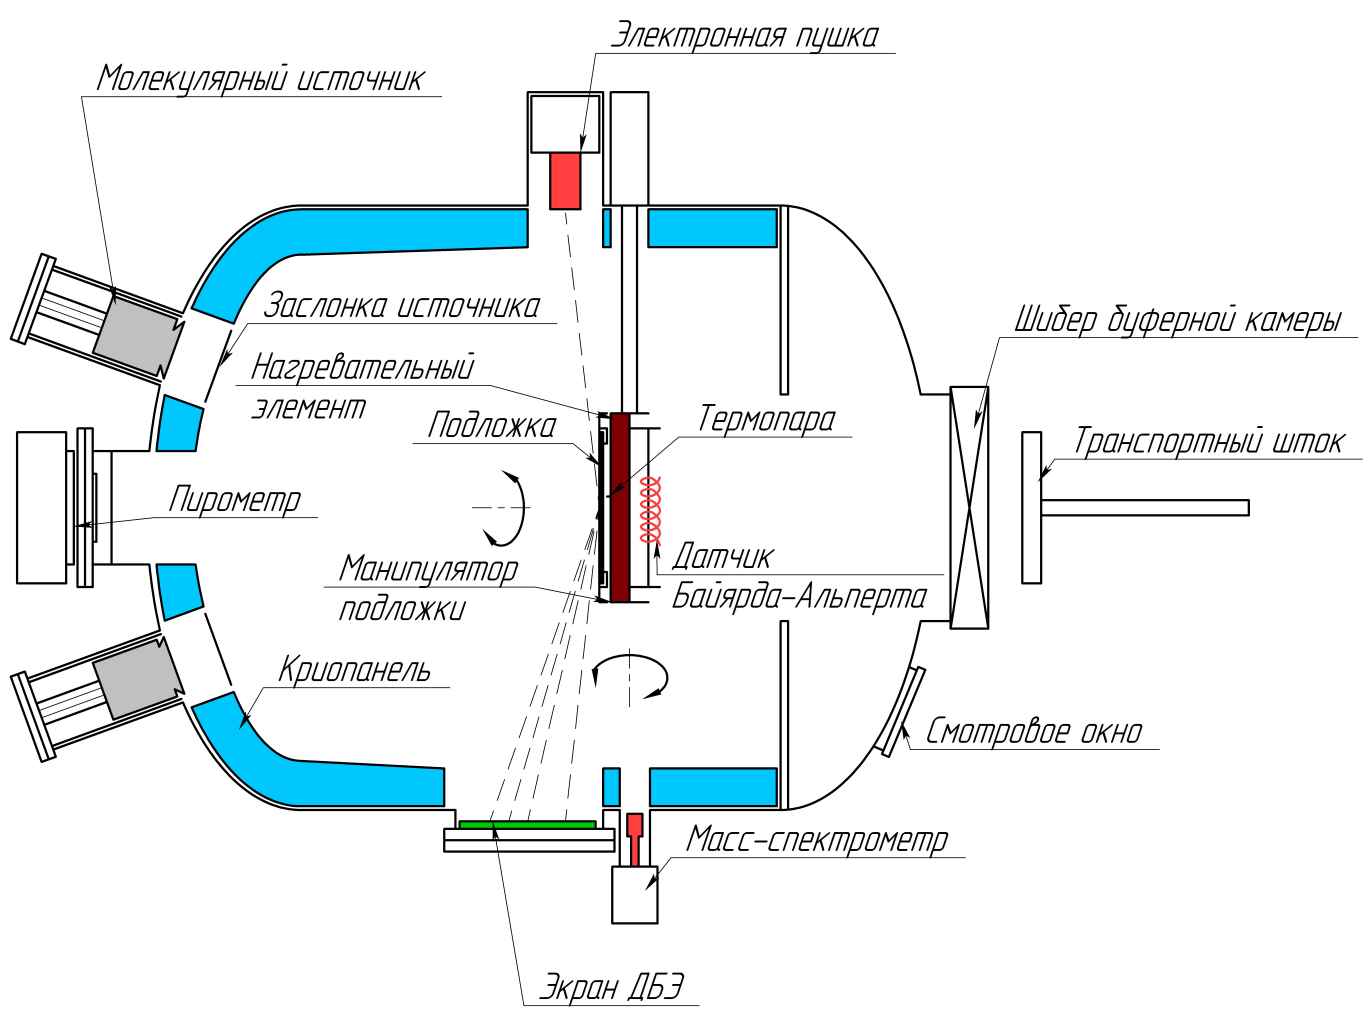
\includegraphics[width=1\linewidth]{Image_11}
} \caption{Схема ростовой камеры установки МПЭ Veeco GEN III, вид
сверху}\label{fig:Image_11} \end{figure}

Источник называют эффузионным, если длина свободного пробега молекул настолько
велика, что их взаимодействием в потоке можно пренебречь. Эффузионный источник
содержит тигель из пиролитического нитрида бора (pBN) с отверстием, в который
загружен испаряемый материал особой чистоты (\(\sim 99,99999\,\%\)). Тигель
окружен нагревательными элементами и охлаждающими трубками с потоком воды или
воздуха. Источники легирующих примесей Si и Be имеют только одну зону нагрева,
а источники элементов III группы имеют две зоны: основания тигля и апертурной
диафрагмы. Температура диафрагмы Ga и In источников поддерживается выше на
100~\si{\degreeCelsius} для предотвращения переконденсации материала на
диафрагму. Это необходимо для обеспечения стабильности потоков и снижения
плотности овальных дефектов. Температура диафрагмы Al источника поддерживается
ниже на 100~\si{\degreeCelsius} для предотвращения вытекания из тигля за счёт
смачивания поверхности pBN. Температура зон контролируется термопарами.
Величина потока регулируется нагревательными элементами и калибруется по
датчику потока перед каждым ростовым процессом. Источники оснащены
пневматическими заслонками для быстрого перекрытия потока.

Давление паров металлов III группы и легирующих примесей, в отличии от
элементов V группы, пренебрежимо мало при температуре синтеза~--- практически
все молекулы потока адсорбируются поверхностью. При росте планарных слоев поток
элементов V группы поддерживают в избытке для недопущения накопления
металлических капель на поверхности подложки из-за температурного разложения. В
таком случае скорость роста определяется потоком элементов III группы.

Управление потоками легколетучих P и As изменением температуры затруднено из-за
инерционности, поэтому крекерные источники P и As на выходе имеют игольчатый
клапан с 300 положениями между закрытым и полностью открытым. В отличие от
металлов III группы, которые испаряются в виде атомов, P и As испаряются в виде
многоатомных молекул \cite{Neave1980}. За игольчатым клапаном находится
крекерная трубка, нагреваемая до высоких температур. Тепловое инфракрасное
излучение поглощается молекулами, разрывая химические связи, таким образом
температура крекерной зоны определяет число атомов в молекулах потока.

В данной работе температура крекерного источника As составляла
600~\si{\degreeCelsius}, что соответствует потоку молекул As\textsubscript{4},
а температура крекерного источника P составляла 900~\si{\degreeCelsius}, что
соответствует потоку молекул P\textsubscript{2}. В конце крекерной зоны
находятся пневматические заслонки для быстрого перекрытия потока.

В крекерный источник P загружают менее химически активную красную аллотропную
модификацию. Давление пара белого P создаёт более стабильный поток, чем
давление пара красного P, поэтому внутри источника находится дополнительно
охлаждаемая область для переосаждения красного P в белый.

Молекулы N\textsubscript{2} имеют высокую энергию связи, поэтому для их
эффективного встраивания применяется источник, в котором поддерживается
высокочастотный (ВЧ) индуктивно-связанный плазменный разряд, в котором
молекулам сообщается дополнительная энергия. Метод роста с применением такого
источника называют молекулярно-пучковой эпитаксии с плазменной активацией азота
(ПА-МПЭ).

C обратной стороны манипулятора находится ионизационный вакуумный датчик
Байярда\,--\,Альперта, который может быть развернут в сторону источников. Он
предназначен для измерения эквивалентного давления пучка (ЭДП) попадающих на
подложку молекул. Из-за различной вероятности ионизации молекул корректно
сравнивать относительную величину потока только молекул одного типа. Различное
расположение источников относительно датчика потока также влияет на показание
датчика потока, на что указывает различная скорость роста при гомоэпитаксии
GaAs/GaAs(001) из разных источников Ga при одинаковых ЭДП в условиях избытка
As.

В некоторых случаях можно определить V/III соотношение ЭДП, при котором адатомы
находятся в стехиометрическом соотношении, наблюдая поверхностный фазовый
переход от обогащённой атомами III группы к обогащённой атомами V группы при
росте планарных слоев (например, в случае гомоэпитаксии GaP и GaAs).
Соотношение V/III ЭДП, при котором происходит поверхностный фазовый переход
зависит от температуры подложки, что, в свою очередь, объясняется зависимостью
отношения между величинами потоков десорбции адатомов V и III групп от
температуры. А следовательно соотношение V/III адатомов в общем случае
нелинейно зависит от соотношения ЭДП V/III.

Абсолютные значения и соотношения V/III ЭДП в схожих процессах на различных
установках МПЭ могут не совпадать, поэтому ориентация на значения потоков, при
которых адатомы находятся в стехиометрическом соотношении, может упростить
перенос ростовой технологии между установками.

\subsection{Дифракция быстрых электронов (ДБЭ)}\label{subsec:ch2/sec1/sub2}

Одно из преимуществ высокого вакуума~--- возможность использовать электронный
пучок для исследования структур в процессе роста. Сочетание относительной
простоты приборной системы и высокой поверхностной чувствительности сделало
метод дифракции быстрых электронов (ДБЭ) постоянным спутником метода МПЭ, а
систему ДБЭ~--- признаком, отличающим МПЭ от других эпитаксиальных методов.

Система ДБЭ состоит из электронной пушки, излучающей фокусируемый поток
электронов, и флуоресцентного экрана. Падая под скользящим углом, пучок
электронов с энергией \(\approx 15\)~\si{\kilo\electronvolt} рассеивается на
кристаллической решётке приповерхностных атомов в сторону флуоресцентного
экрана. По дифракционной картине можно судить о кристаллической структуре
поверхности, её реконструкции и структурном совершенстве, времени формирования
монослоя, морфологии наноструктур и наличии двойникования.

Рассеянные электроны конструктивно интерферируют при выполнении условий Лауэ:

\begin{equation} \label{eq:eq_2} \vec{k} - \vec{k_0} = m\vec{q}, \end{equation}
где \(\vec{k}\)~--- волновой вектор дифрагированной волны, \(\vec{k_0}\)~---
волновой вектор падающей волны, \(m\)~--- целое число, \(\vec{q}\)~--- вектор
обратной решётки.

В обратном пространстве через начало координат можно построить сферу отражения
радиусом \(| \vec{k} |\) с центром в начале вектора \(\vec{k}\). Данное
построение называют построением сферы Эвальда. Волновой вектор дифрагированных
волн, а с ним и картину дифракции, можно найти, построив вектора из центра
сферы Эвальда с концами в узлах обратной решётки, который пересекается сферой
Эвальда.

Обратная решётка от двумерной периодической структуры атомов представляет собой
множество бесконечно длинных стержней (тяжей), перпендикулярных к плоскости
атомов. Поэтому в случае кристаллической, атомарно гладкой поверхности сфера
Эвальда пересекает тяжи, что соответствует дифракционной картине из серии полос
с модулированной интенсивностью, наложенных на фон из-за неупругого рассеяния.

Если поверхность не гладкая, электроны рассеиваются сквозь неровности, в
результате чего образуется пятнистая дифракционная картина из рефлексов
(аналогично дифракции рентгеновских лучей на трёхмерной кристаллической
решётке), удлинённых в направлении нарушения кристаллической симметрии. Это
позволяет различить тонкие и широкие нанообъекты. Дифракция от аморфной
поверхности (например, от поверхностного оксида) формирует размытый диффузный
фон, а от поликристаллической поверхности~--- набор колец (аналогично
порошковым дифрактограммам).

Упорядочение поверхностных атомов может существенно отличаться от объёмного. В
результате поверхностной реконструкции формируется сверхструктура, базисная
ячейка которой обычно кратна элементарной ячейке исходной структуры. Когда углы
между векторами трансляции элементарных ячеек поверхности и подложки совпадают,
для обозначения сверхструктуры используют запись вида \begin{equation}
\label{eq:eq_3} \frac{a_{1s}}{a_{2b}} \times
\frac{a_{2s}}{a_{2b}}-R\phi\si{\degree}, \end{equation} где \(a_{1s}\) и
\(a_{2s}\)~--- вектора трансляции элементарной поверхностной ячейки, \(a_{1b}\)
и \(a_{2b}\)~--- вектора трансляции элементарной нижележащей ячейки,
\(\phi\si{\degree}\)~--- угол поворота ячейки.

Так как расстояние между дифракционными полосами обратно пропорционально
размеру элементарной ячейки поверхностной решётки, сверхструктура на картине
дифракции проявляется как набор полос между основными рефлексами.

Адсорбция на поверхности атомов также может способствовать поверхностному
фазовому переходу \cite{Bringans1993, Ji2007}. Адсорбируюсь, As пассивирует
поверхность Si\((111)7\)\(\times\)\(7\), образуя сверхструктуру
Si\((111)1\times1-\text{As}\) \cite{Patel1989, Bringans1992}, а P (из-за
больших поверхностных растягивающих напряжений) образует неупорядоченную
несоразмерную сверхструктуру
Si\((111)6\sqrt{3}\)\(\times\)\(6\sqrt{3}-R30\si{\degree}-\text{P}\)
\cite{Vitali1998, Siriwardena2017}. Ga образует различные сверхструктуры при
эквивалентной толщине менее монослоя, а при эквивалентных толщинах более
монослоя~--- образует капли (см.~рис.~\cref{fig:Image_12}) \cite{Park1988},
которые могут служить катализатором для роста в режиме ПЖК
(см.~подраздел~\cref{subsec:ch1/sec2/sub2}) или участвовать в капельной
эпитаксии (см.~подраздел~\cref{subsec:ch1/sec2/sub6}). Эквивалентный монослой
здесь означает \(6,8 \cdot 10^{14}\)~атомов\si{\per\centi\meter^{2}}~---
поверхностная плотность объёмного Si толщиной монослой на поверхности (111)
\cite{Kumar2010}.

\begin{figure}[ht] \centerfloat{
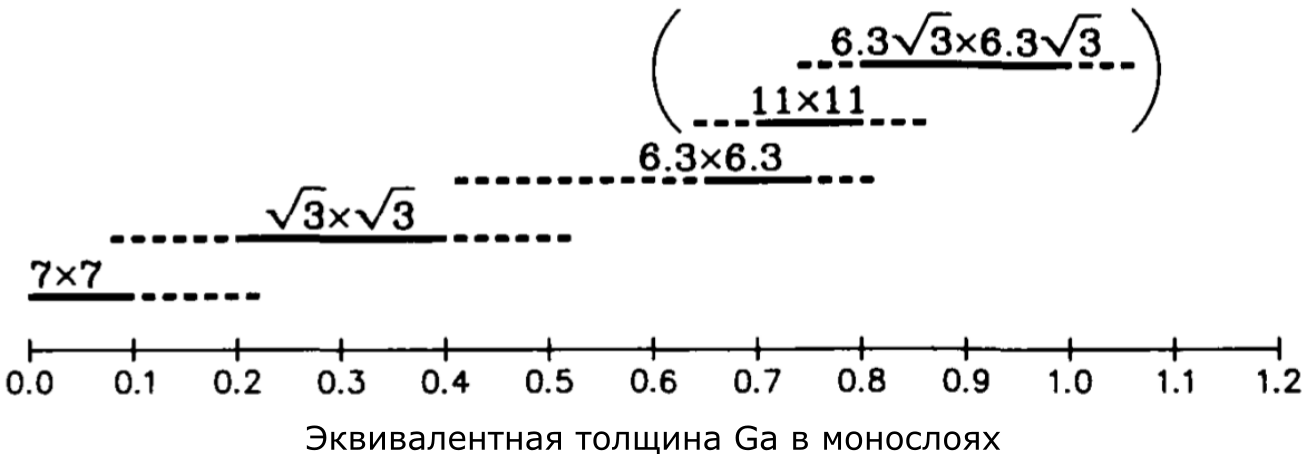
\includegraphics[width=0.8\linewidth]{Image_12} } \caption{Фазовая диаграмма Ga
на Si(111) \cite{Park1988}}\label{fig:Image_12} \end{figure}

В начале послойного роста, пока рост когерентен в области под электронным
пучком, интенсивность дифракционных линий осциллирует с периодом равным времени
формирования одного монослоя \cite{Harris1981}. Интенсивность рефлексов
максимальна, когда поверхность атомарно гладкая. Если зарождение происходит на
атомных террасах, то рассеяние от атомов поверхности и зародышей вызывает
деструктивную интерференцию, поэтому интенсивность рефлексов минимальна, когда
монослой заполнен наполовину. Осцилляции интенсивности не наблюдаются при росте
в режиме встраивания адатомов в край ступени «step-flow» (так как поверхность
сохраняет свою гладкость) и в случае роста объёмных наноструктур.

\section{Постростовые методы исследования}\label{sec:ch2/sec2}

\subsection{Растровая (РЭМ) и просвечивающая (ПЭМ) электронная
микроскопия}\label{subsec:ch2/sec2/sub1}

Иногда морфологию нанообъектов можно оценить методом оптической спектроскопии
даже если их размеры в одном или двух направлениях меньше дифракционного
предела, например, в целях определения длины, направления роста и плотности
ННК. Для получения изображений большего разрешения используются микроскопы с
пучком электронов вместо светового потока.

В растровых электронных микроскопах (РЭМ) сфокусированный электронный пучок
(диаметр \(\approx 1~\si{\nano\meter}\)) сканирует поверхность образца, при
взаимодействии с которым генерируются вторичные электроны и характеристическое
рентгеновское излучение, которые собираются детекторами. Интенсивность сигнала
зависит от природы вещества, что в некоторых случаях позволяет различать фазы с
разным химическим составом (например, включения GaPAs в ННК GaP), и топографии
в области взаимодействия. По спектру характеристического рентгеновского
излучения можно судить о концентрации химических элементов в образце.

В просвечивающих электронных микроскопах (ПЭМ) электронный поток, проходя
сквозь образец, неоднородно поглощается и рассеивается, после чего фокусируется
электронной оптикой на детекторе. Фокусное расстояние промежуточной линзы можно
менять так, чтобы на флуоресцентном экране фокусировалась или плоскость объекта
(для формирования его увеличенного изображения), или задняя фокальная плоскость
(для формирования картины микродифракции участка под электронным пучком).

Исследуемая область образца должна быть достаточно тонкой, порядка десятков нм,
поэтому образцы толще \(\approx 100~\si{\nano\meter}\) подготавливают
полировкой и ионным распылением.

Просвечивающий растровый электронный микроскоп (ПРЭМ)~--- вид ПЭМ, в котором
для увеличения разрешения пучок электронов фокусируют в точку размером
\(\approx 0,05~\si{\nano\meter}\), которой проводят растровое сканирование
поверхности образца.

При съёмке в светлопольном (bright field) режиме на детекторе собираются
электроны вблизи оси пучка. В этом случае на контраст в большей степени влияет
толщина, плотность, состав и кристаллическая структура исследуемого объекта:
области с большей толщиной и большим атомным номером имеют тёмный контраст
из-за неупругого рассеяния проходящих через образец электронов.

В темнопольном (dark field) режиме на детекторе, из-за введённой в фокальную
плоскость апертуры, собираются только определённые дифрагированные электроны. В
этом случае изображение чувствительно к кристаллической ориентации и дефектам
решётки.

Режим высокоразрешающей электронной микроскопии (ВРЭМ), в котором падающий
пучок электронов ориентирован параллельно оси зоны кристалла, позволяет изучать
кристаллическую структуру и дефекты с атомным разрешением
(\(\approx0,05~\si{\nano\meter}\)). Изображения ВРЭМ могут выглядеть, как
изображения атомной решётки, однако контраст создаётся интерференцией
дифрагированных лучей, поэтому изображения ВРЭМ следует интерпретировать с
осторожностью.

\subsection{Атомно-силовая микроскопия (АСМ)}\label{subsec:ch2/sec2/sub2}

Метод атомно-силовой микроскопии (АСМ) основан на регистрации взаимодействия
между поверхностью образца и остриём зонда для исследования рельефа и локальных
физических свойств поверхности. На воздухе данный метод позволяет исследовать
атомные ступени, а в условиях высокого вакуума в состоянии обеспечить реальное
атомное разрешение с визуализацией атомной реконструкции.

Зонд имеет конструкцию кантилевера, и представляет собой балку, один конец
которой жёстко закреплён, а на другом перпендикулярно выступает острие с
радиусом закругления 1--90~\si{\nano\meter}. Сила взаимодействия, действующая
на острие со стороны поверхности, изгибает балку, что регистрируется по
отклонению отражённого от балки луча лазера. Образец во время сканирования
перемещается пьезодвигателем во всех направлениях. В результате на изображении
АСМ каждой точке поверхности присваивается значение высоты рельефа.

Стремление улучшить латеральное разрешение привело к развитию полуконтактного
метода, при котором расстояние зонда до поверхности такое, что на него
действует как отталкивание, так и притяжение. Пьезоэлектрический вибратор, к
которому прикладывается гармоническое напряжение, возбуждает колебания
кантилевера на частоте близкой к резонансной с соответствующей амплитудой
свободных колебаний. Амплитуда колебаний зонда уменьшается с приближением до
поверхности из-за взаимодействия. Во время растрового сканирования из-за
неровностей рельефа расстояние зонда до поверхности изменяется, а
следовательно, и амплитуда колебаний. Это изменение расстояния компенсируется
системой обратной связи так, чтобы амплитуда колебания зонда оставалась
постоянной.

\subsection{Спектроскопия фотолюминесценции (ФЛ)}\label{subsec:ch2/sec2/sub3}

Метод спектроскопии фотолюминесценции (ФЛ) основан на явлении
фотолюминесценции~--- свечении, возбуждаемом светом. Это один из основных
методов изучения оптических свойств и структуры энергетических уровней
полупроводника.

Полупроводниковый образец облучается лазерным излучением с энергией фотонов
больше ширины запрещённой зоны, при этом генерируются неравновесные
электронно-дырочные пары, которые рассеивают часть своей энергии, а затем
рекомбинируют (как излучательно, так и безызлучательно). Длины волн и
интенсивность фотонов, испущенных данным образцом, регистрируются системой из
монохроматора и фотодетектора. Тепловые колебания кристаллической решётки
увеличивают вероятность безызлучательной рекомбинации, поэтому, как правило, ФЛ
при охлаждении образца становится ярче.

Электрон и дырка могут образовать экситон~--- связанное водородоподобное
состояние, устойчивое благодаря кулоновскому взаимодействию. Энергия
образования экситона меньше ширины запрещённой зоны на энергию связи электрона
и дырки, поэтому на спектрах ФЛ линии экситонного излучения смещены от края
зоны поглощения в сторону длинных волн. Свободный электрон может быть захвачен
нейтральным или ионизированным примесным атомом, образуя связанный на примеси
экситон. В таком случае линия экситонного излучения смещается в сторону длинных
волн от линии излучения свободных экситонов на энергию связи экситона с атомом
примеси.

В объёмных материалах экситонные состояния проявляются при низких температурах,
однако в наноразмерных структурах могут наблюдаться при комнатной температуре.

\subsection{Спектроскопия комбинационного рассеяния света
(КРС)}\label{subsec:ch2/sec2/sub4}

Комбинационное рассеяние света (КРС)~--- это неупругое рассеяние света
веществом с возбуждением или релаксацией собственных молекулярных колебаний
(мод). В случае твёрдого тела оно сопровождается рождением (стоксов процесс)
или уничтожением фононов (антистоксов процесс).

Как правило, в спектроскопии КРС проявляются колебания, при которых изменяется
поляризуемость связи, тогда как в инфракрасной спектроскопии проявляются
колебания с изменением дипольного момента связи. Величина рассеянной или
приобретённой фотоном энергии соответствует энергии фононов вблизи центра зоны
Бриллюэна. По интенсивности и величине сдвига можно сделать выводы о химическом
составе, кристаллической структуре и упругих напряжениях.

В резонансной спектроскопии КРС энергия возбуждающего фотона совпадает с
энергией электронного перехода материала образца. Электронное возбуждение может
повысить поляризуемость связи, и, следовательно, интенсивность сигнала КРС.

Установка спектроскопии КРС может быть объединена с установкой спектроскопии ФЛ
при условии высокой разрешающей способности монохроматора и детектора (\(<
1~\si{\per\centi\meter}\)).

\FloatBarrier
           % Глава 2
\chapter{Капельная эпитаксия GaN триподов}\label{ch:ch3}

При обычных условиях GaN~--- прямозонный полупроводник с шириной запрещённой
зоны \(\approx 3,4\)~\si{\electronvolt} и WZ кристаллической структурой. Он
широко используется при изготовлении оптоэлектронных приборов ультрафиолетового
диапазона, белых светодиодов, сверхвысокочастотных транзисторов, мощных диодов.

В данной главе излагаются результаты исследования влияния затравки из островков
GaN, полученных методом капельной эпитаксии, на морфологию и поверхностную
плотность наноструктур GaN, синтезированных методом ПА-МПЭ. Показано, что
использование данной затравки \cite{Debnath2009, Yu2014} приводит к
формированию ориентированного массива из трёх типов наноструктур: Y-образных
наноостровков (триподов), вертикальных и наклоненных ННК.

\section{Постановка эксперимента}\label{sec:ch3/sec1}

Наноструктуры GaN выращены методом ПА-МПЭ на установке Veeco GEN III. Данная
установка оборудована радиочастотным плазменным источником азота Riber
(13,56~\si{\mega\hertz}). Параметры источника азотной плазмы во время
нитридации и роста GaN оставались неизменными: поток азота~--
1~\si{\centi\meter^3\per\minute}; подводимая ВЧ мощность~--- 500~\si{\watt}.
Отраженная мощность поддерживалась ниже 1~\si{\watt} устройством
автоматического согласования импедансов. Интенсивность плазмы измерялась
кремниевым фотодиодом. Спектр излучения плазмы имеет линии, соответствующие
атомарному азоту и возбуждённым молекулам N\textsubscript{2}
\cite{Debnath2016}. Для увеличения угловой однородности и устранения ионов в
потоке плазмы источник имеет дополнительную диафрагму из молибдена. Для синтеза
использовались Si(111) подложки p-типа с углом разориентации 4{\textdegree} в
направлении <110>\textsubscript{Si}. Перед загрузкой в установку МПЭ подложки
подготавливались по методу Шираки \cite{Ishizaka2019}. Температура подложки
контролировалась термопарой с обратной стороны подложки и пирометром.
Термическим отжигом подложки (10~\si{\minute} при 850~\si{\degreeCelsius})
достигалась атомарная чистота поверхности Si, что подтверждено реконструкцией
Si\((111)7\)\(\times\)\(7\) на картине ДБЭ и гладкой морфологией поверхности на
АСМ изображениях.

ЭДП азота находилось в диапазоне от \(2 \cdot 10^{-7}\) до \(3 \cdot
10^{-7}\)~\si{\torr}. Для поддержания богатых азотом условий ЭДП Ga
поддерживалось достаточно малым~--- в диапазоне от \(1 \cdot 10^{-8}\) до \(2
\cdot 10^{-8}\)~\si{\torr}, что соответствует скорости роста
25--50~\si{\nano\meter\per\hour} при гомоэпитаксии планарного GaAs в избытке
As.

Затравочные капли Ga осаждались до зажигания азотной плазмы на поверхностной
реконструкции Si\((111)7\)\(\times\)\(7\) при температуре подложки
200~\si{\degreeCelsius}. Эквивалентная толщина Ga оценивалась по наблюдаемой на
ДБЭ реконструкции поверхности. На поверхности Si(111) 0,3~монослоя Ga образует
реконструкцию Si\((111)\sqrt{3}\)\(\times\)\(\sqrt{3} - R30\si{\degree} -
\text{Ga}\) \cite{Kawazu1988}, а 0,6~монослоя~--- несоразмерную реконструкцию
Si\((111)6,3\)\(\times\)\(6,3 - \text{Ga}\) \cite{Cechal2007}. При
эквивалентной толщине (объем материала, нормированный на площадь поверхности)
Ga более 1,5~монослоев на картине ДБЭ наблюдаются диффузные полукруглые гало,
вызванные каплями Ga на поверхности. Монослой здесь означает \(6,8 \cdot
10^{14}\)~атомов\si{\per\centi\meter^{2}}~--- поверхностная плотность объёмного
Si толщиной монослой на поверхности (111)
(см.~подраздел~\cref{subsec:ch2/sec1/sub2}) \cite{Kumar2010}. Низкая
температура подложки и малый объем наносимого Ga были выбраны для получения
плотного массива наноразмерных капель \cite{Ristic2008}. Большая толщина
зародышевого слоя и высокие температуры осаждения не использовались, чтобы
избежать образования эвтектического раствора Ga\,--\,Si, травления и
нежелательного Ga легирования подложки Si \cite{Yamane2009, Dadgar2015}. После
нанесения Ga капель подложка нагревалась под потоком активированного в плазме
азота до температуры роста (690--710~\si{\degreeCelsius}). После выдержки под
азотом открывалась заслонка Ga источника для синтеза GaN.

Морфология синтезированных наногетероструктур изучена методом PЭМ (Zeiss SUPRA
25) и АСМ (Bruker Bioscope Catalyst SPM). Исследования методом ВРЭМ проводились
на микроскопе Jeol JEM-2100F (рабочее напряжение 200~\si{\kilo\volt},
разрешение от точки до точки 0,19~\si{\nano\meter}). Образцы для исследований
ВРЭМ подготовлены механическим полированием с последующим ионным распылением
Ar\textsuperscript{+}. Исследование особенностей ФЛ проводилось при температуре
10~\si{\kelvin} с возбуждением на длине волны 325~\si{\nano\meter} с
использованием HeCd лазера и детектора PMI Hamamatsu R298.

\section{Нитридация Ga капель}\label{sec:ch3/sec2}

Морфология капель Ga эквивалентной толщиной 1,35~монослоя на вицинальной
Si(111) подложке исследована методом АСМ (см.~рис.~\cref{fig:Image_13_1}).
Из-за разориентации 4{\textdegree} высокотемпературный отжиг кремниевой
подложки приводит к эшелонированию ступеней~--- образованию эшелонов близко
расположенных ступеней, разделённых крупными террасами с пониженной плотностью
атомных ступеней \cite{Latyshev1998, Hibino1994}. Нанесённые капли Ga высотой
около 2--3~\si{\nano\meter} располагаются по краям атомно гладких террас (см.
вставка на~рис.~\cref{fig:Image_13_1}). Среднее расстояние между каплями
составляет 100~\si{\nano\meter}.

\begin{figure}[ht] \centerfloat{ \subcaptionbox{\label{fig:Image_13_1}}{%
			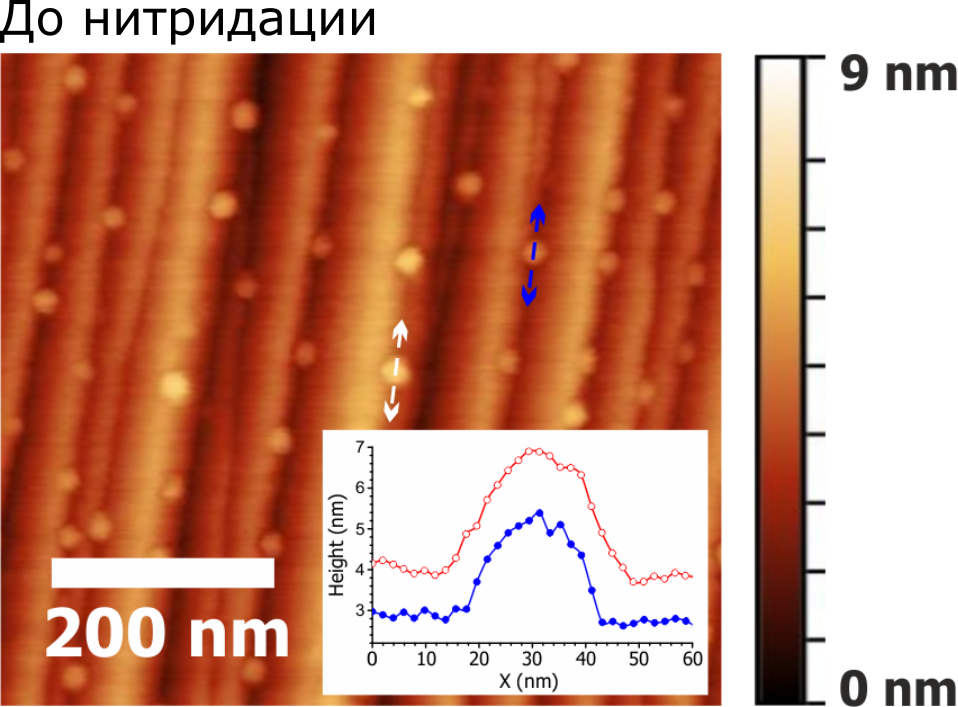
\includegraphics[width=0.45\linewidth]{Image_13_1}}
			\subcaptionbox{\label{fig:Image_13_2}}{%
			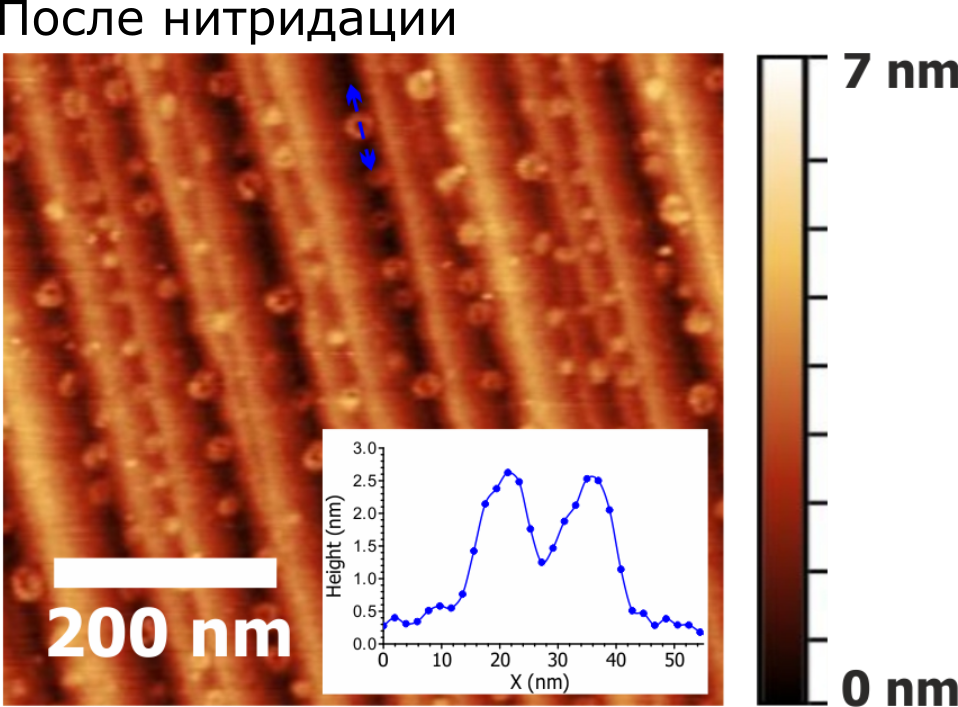
\includegraphics[width=0.45\linewidth]{Image_13_2}} }
			\legend{Разориентация поверхности 4{\textdegree} в направлении <110>. На
				вставках представлены профили АСМ сканирования наноструктур}
				\caption{АСМ изображения поверхности Si подложки с каплями Ga
			(эквивалентной толщины 1,35~монослоя) до нитридации~(а) и после
	нитридации~(б)}\label{fig:Image_13} \end{figure}

Под потоком активированного азота капли кристаллизуются в кольцо высотой
1--2~\si{\nano\meter} и глубиной центрального углубления
0,5--1~\si{\nano\meter} (см. вставки на~рис.~\cref{fig:Image_13}). Схожая
морфология может быть получена капельной эпитаксией GaAs \cite{Zhou2013} и
связана с локализованным ростом соединений
A\textsuperscript{III}B\textsuperscript{V} за счет более быстрого
зародышеобразования вдоль края капли
(см.~подраздел~\cref{subsec:ch1/sec2/sub6}). После нитридации островки обладают
меньшей высотой и повышенной поверхностной плотностью по сравнению с исходными
каплями, что указывает на продолжение диффузия Ga под потоком активного азота.

Исследование ПЭМ не показало травление подложки галлием
(см.~раздел~\cref{sec:ch3/sec4}). Морфология поверхности с нитридированными
нанокольцами не изменилась после воздействия водного раствора соляной кислоты,
что указывает на отсутствие металлического Ga или эвтектического раствора Si-Ga
на поверхности после нитридации.

\section{Кристаллографические ориентации триподов}\label{sec:ch3/sec3}

Синтез GaN ННК на подложке с нитридированными каплями Ga может приводить к
формированию дополнительного массива наноструктур~--- ориентированных
наноостровков GaN в форме трипода (см.~рис.~\cref{fig:Image_14_12}).  Триподы
образованы тремя вытянутыми ветвями, расположенными под углом 120{\textdegree}
друг к другу. По отношению к базовому срезу подложки можно определить
эпитаксиальную ориентацию триподов к решётке Si: триподы имеют предпочтительную
ориентацию в плоскости подложки с выравниванием ветвей вдоль
кристаллографических направлений <\(1\overline{1}0\)>\textsubscript{Si},
<\(11\overline{2}\)>\textsubscript{Si}, <\(12\overline{3}\)>\textsubscript{Si}.
Эти ориентации показаны на рисунке~\cref{fig:Image_14_3} с указанием
пунктирными линиями кристаллических двойников, соответствующих повороту на
180{\textdegree} в плоскости подложки. Некоторые триподы имеют только одну или
две ветви.

\begin{figure}[ht] \centerfloat{ \subcaptionbox{\label{fig:Image_14_1}}{%
			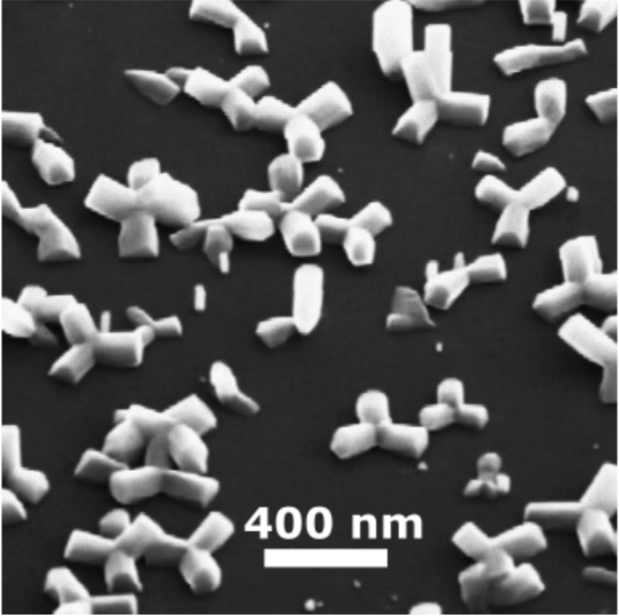
\includegraphics[width=0.4\linewidth]{Image_14_1}}
			\subcaptionbox{\label{fig:Image_14_2}}{%
			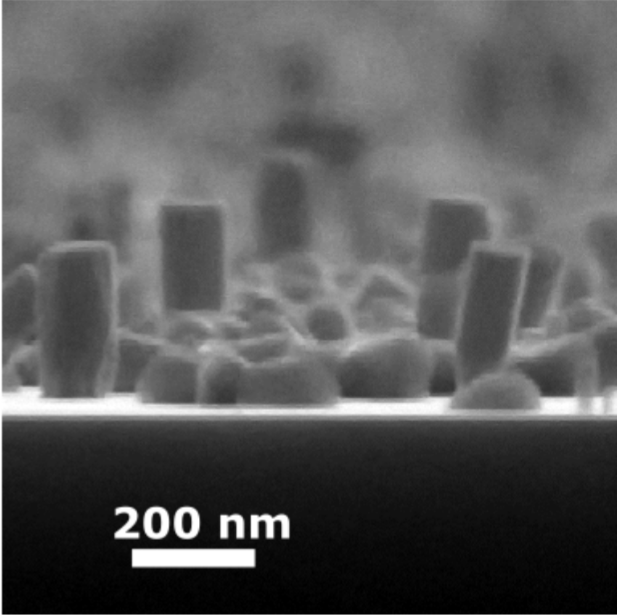
\includegraphics[width=0.4\linewidth]{Image_14_2}} }
			\legend{Изометрический вид~(а), вид сбоку~(б)} \caption{РЭМ изображения
		эпитаксиальных нанотриподов GaN}\label{fig:Image_14_12} \end{figure}

\begin{figure}[ht] \centerfloat{
		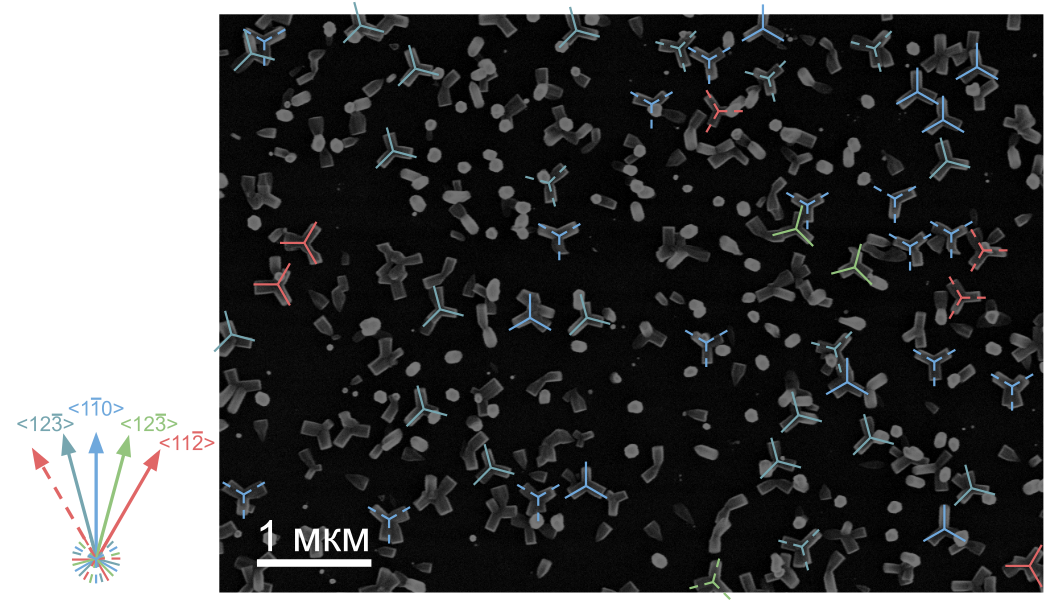
\includegraphics[width=1\linewidth]{Image_14_3} } \legend{Ориентации
		триподов схематически обозначены цветными символами. Кристаллографические
		направления указаны на схеме слева} \caption{РЭМ изображение эпитаксиальных
нанотриподов GaN, вид сверху}\label{fig:Image_14_3} \end{figure}

Формирование подобных GaN триподов уже было исследовано в ряде работ: на
c-плоскости Al\textsubscript{2}O\textsubscript{3} методом хлорид-гидридной
газофазной эпитаксии \cite{Lee2010}, на наноколоннах GaN методом ПА-МПЭ
\cite{Wang2017}, на алмазной подложке методом селективной эпитаксии
\cite{Schuster2015}.

\section{Исследование кристаллической структуры методом
ПЭМ}\label{sec:ch3/sec4}

На подложке с поверхностной реконструкцией Si\((111)6,3\)\(\times\)\(6,3 -
\text{Ga}\) синтезирован массив наноструктур (см.~раздел~\cref{sec:ch3/sec1}).
На гетероинтерфейсе GaN/Si (см.~рис.~\cref{fig:Image_15_1}) наблюдается
аморфный слой толщиной \(\approx 1,5\)~\si{\nano\meter}. Данный слой может быть
аморфным SiN\textsubscript{x}, который может формироваться в процессе
нитридации затравочных капель при взаимодействии поверхности Si с активным
азотом. У данного процесса существует несколько механизмов: до насыщения азотом
и образования зародыша капли Ga мигрируют по поверхности Si, которая уже
провзаимодействовала с потоком азота; в процессе насыщения капли Ga часть
растворенных молекул азота взаимодействует с поверхностью подложки под каплей;
адомы азота диффундируют в приповерхностном слое Si \cite{Rawdanowicz2004}.

\begin{figure}[ht] \centerfloat{ \subcaptionbox{\label{fig:Image_15_1}}{%
			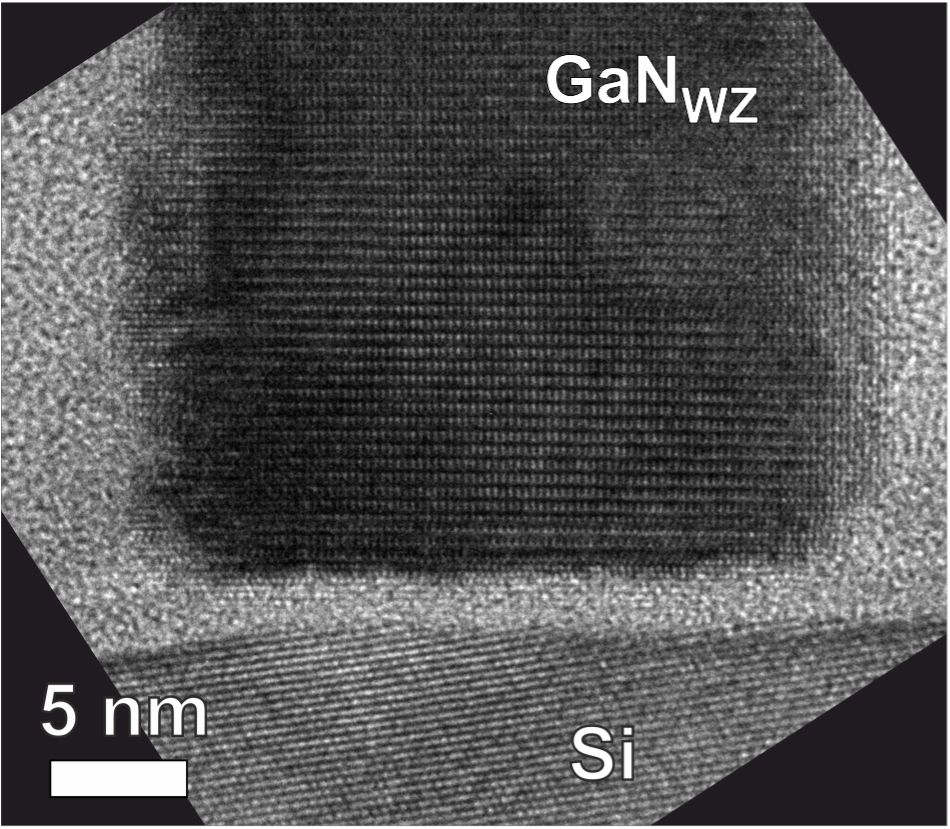
\includegraphics[height=7cm]{Image_15_1}}
			\subcaptionbox{\label{fig:Image_15_2}}{%
			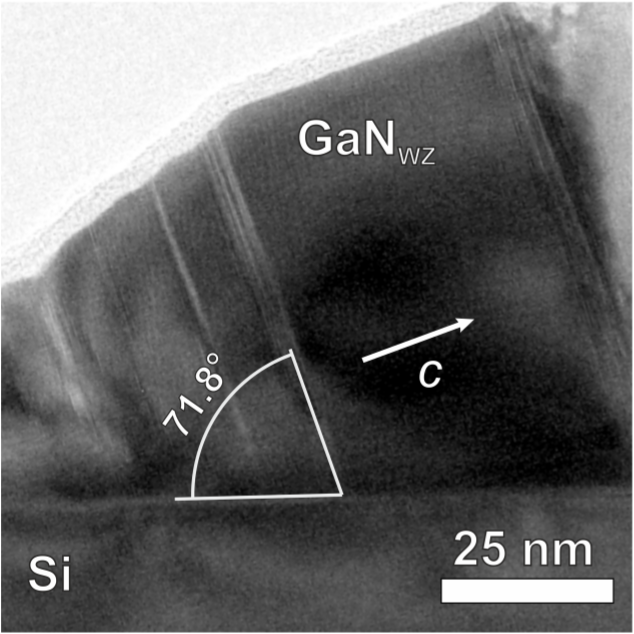
\includegraphics[height=7cm]{Image_15_2}} } \caption{ВРЭМ изображение
		гетероинтерфейса вертикального ННК GaN с подложкой Si(111)~(а), ПЭМ
	изображение ветви трипода GaN на подложке Si(111)~(б)}\label{fig:Image_15}
\end{figure}

Согласно работе \cite{Lee2010}, формирование нанотриподов GaN начинается с
образования ZB наноостровка с последующим зарождением и ростом в плоскости
подложки WZ наностержней на его \{111\} фасетках. Изучение триподов методом ПЭМ
затруднено формированием муарового контраста от наложения решёток ветви и ядра,
поэтому выводы о структуре ядра триподов были сделаны на основе изучения схожих
объектов массива.

При изучении ПЭМ изображений образца были обнаружены наклонный ННК и ветвь
нанотрипода с общим ядром (см.~рис.~\cref{fig:Image_16}). На картинах
электронной микродифракции этих структур были видны рефлексы только WZ
структуры GaN, так как интенсивность рассеяния на ядре наночастицы была
недостаточной для регистрации из-за ее малого объёма.

Упаковка кристаллической решётки WZ и ZB была различима на изображениях ВРЭМ с
ориентацией образца вдоль оси зоны
\([\overline{1}2\overline{1}0]\)\textsubscript{WZ GaN}. Изображения быстрого
преобразования Фурье (БПФ) от отмеченных пунктирными квадратами областей
наноструктуры с различными упаковками представлены
на~рис.~\cref{fig:Image_16_2}. Расчётные сечения обратного пространства WZ и ZB
структур с соответствующими осями зон
\([\overline{1}2\overline{1}0]\)\textsubscript{WZ GaN} и
\([\overline{11}0]\)\textsubscript{ZB GaN} отмечены на изображениях БПФ
оранжевыми и белыми пунктирными кружками соответственно.

\begin{figure}[ht] \centerfloat{ \subcaptionbox{\label{fig:Image_16_1}}{%
			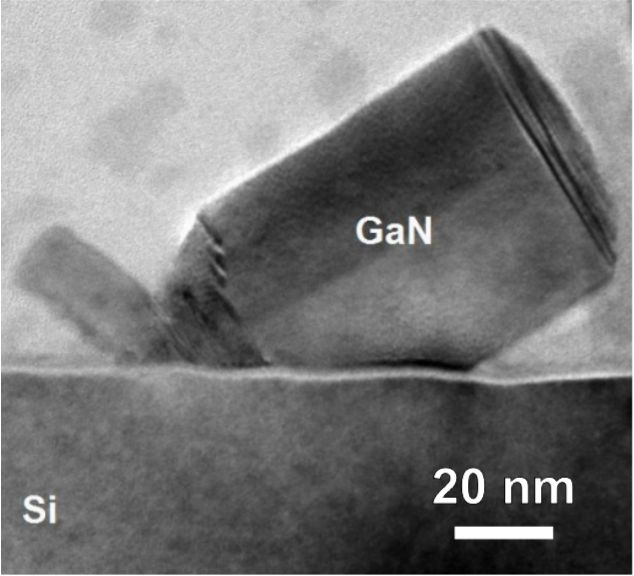
\includegraphics[height=8cm]{Image_16_1}}
			\subcaptionbox{\label{fig:Image_16_2}}{%
			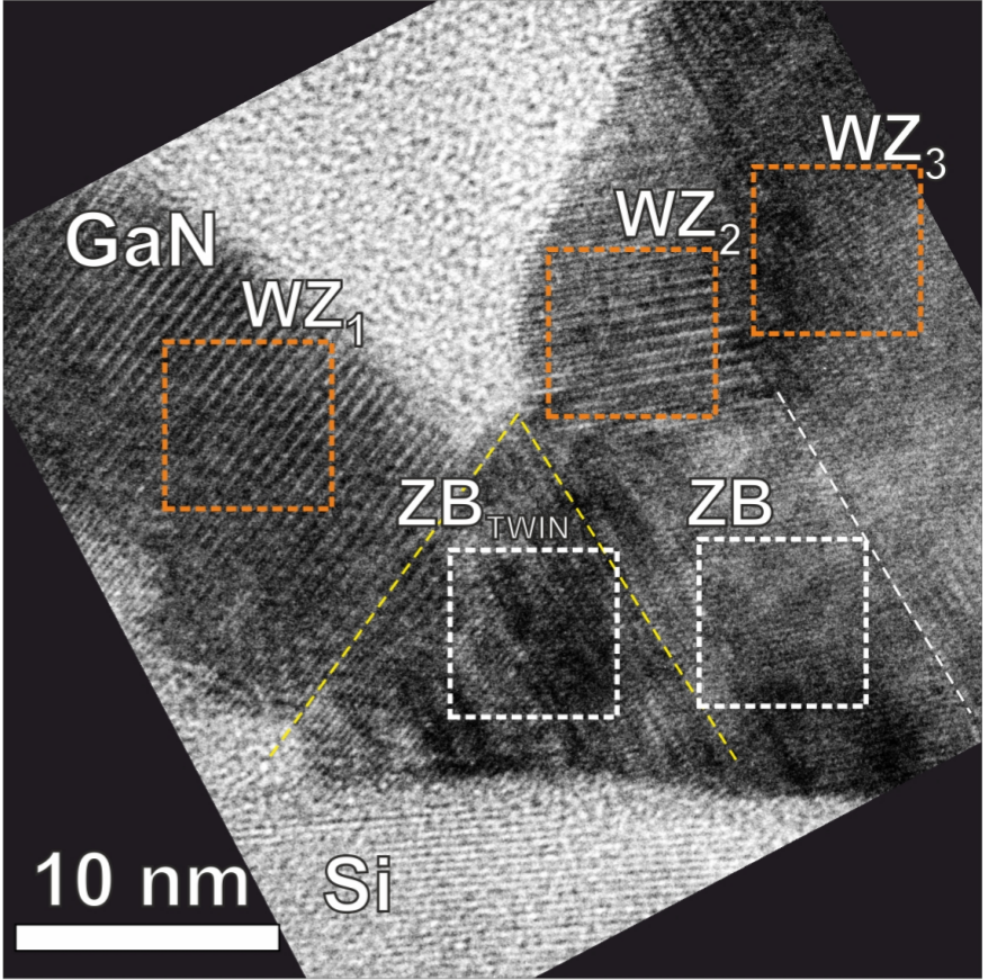
\includegraphics[height=8cm]{Image_16_2}}

		\subcaptionbox{\label{fig:Image_16_3}}{%
			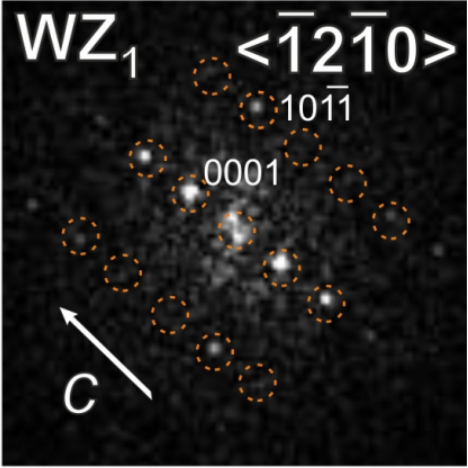
\includegraphics[width=0.19\linewidth]{Image_16_3}}
			\subcaptionbox{\label{fig:Image_16_4}}{%
				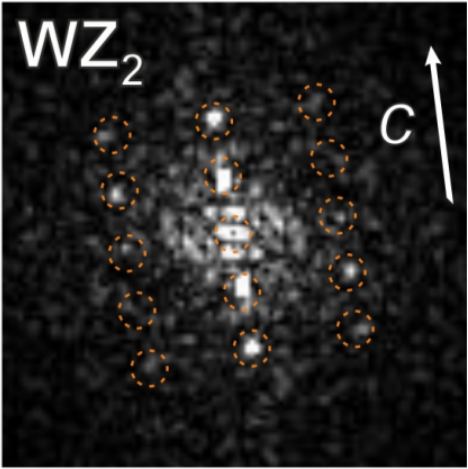
\includegraphics[width=0.19\linewidth]{Image_16_4}}
				\subcaptionbox{\label{fig:Image_16_5}}{%
				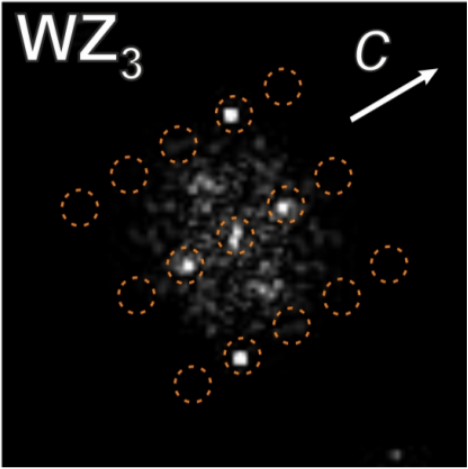
\includegraphics[width=0.19\linewidth]{Image_16_5}}
				\subcaptionbox{\label{fig:Image_16_6}}{%
					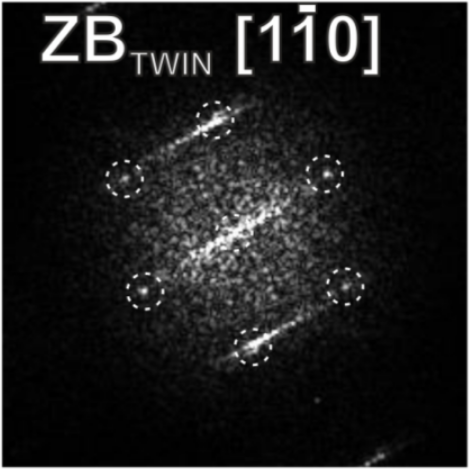
\includegraphics[width=0.19\linewidth]{Image_16_6}}
					\subcaptionbox{\label{fig:Image_16_7}}{%
				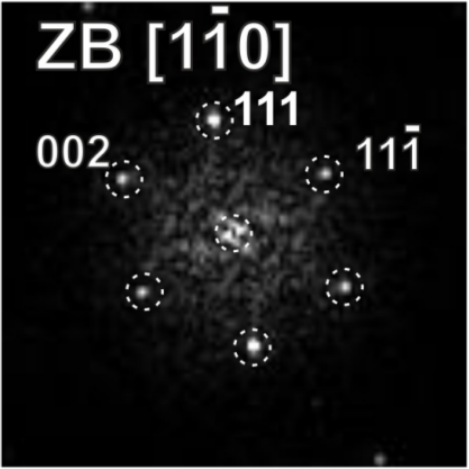
\includegraphics[width=0.19\linewidth]{Image_16_7}} }
				\caption{Микроснимок ПЭМ наклонного ННК и ветви трипода GaN с общим
					центром~(а). Вид крупным планом ВРЭМ~(б) с соответствующими
			изображениями БПФ от областей, отмеченных пунктирными
	квадратами~(в\,--\,ж)}\label{fig:Image_16} \end{figure}

В результате БПФ анализа отчётливо видно отличие кристаллической структуры
основания от ветви и наклонного ННК: наиболее заметное отличие~---
периодичность и симметрия БПФ образа, соответствующая гексагональной и
кубической последовательности укладки плотно упакованных плоскостей
\cite{Jo2018, Bayram2014}. В базовой части (отмечена
на~рис.~\cref{fig:Image_16_2} как ZB и ZB\textsubscript{twin}) периодичность
типа ABCABC{\dots} соответствует GaN со структурой ZB (вдоль <111>). Каждая из
букв A, B и C обозначает бислой атомов, состоящий из одного слоя с атомами
группы III и одного слоя с атомами группы V. У наклонного ННК и ветви
(обозначены на~рис.~\cref{fig:Image_16_2} как WZ\textsubscript{1},
WZ\textsubscript{2}, WZ\textsubscript{3}) периодичность типа ABAB{\dots}
соответствует GaN со структурой WZ (вдоль <0001>) \cite{Kriegner2011}.

Таким образом, WZ триподы и наклонные ННК имеют в основании ZB наноостровок. В
простейшем случае он имеет тетраэдрическую форму с гранями
\{111\}\textsubscript{ZB GaN}, плоскость (111)\textsubscript{ZB GaN} которых
ориентирована параллельно Si(111). Такое ZB ядро служит центром
зародышеобразования трипода или наклонённого ННК. Вертикальные ННК
(см.~рис.~\cref{fig:Image_15_1}) не имеют в основании затравочных островков.

Зарождение метастабильной ZB структуры GaN связывают с низкой температурой
роста или избытком Ga \cite{Shi2006, Romano1997}. Аналогичное образование ННК
InAs с метастабильной WZ структурой объясняют размерными эффектами
\cite{Johansson2010}.

Яркие полосы вдоль направления \([11\overline{1}]\) на БПФ образе области
ZB\textsubscript{twin} (см.~рис.~\cref{fig:Image_16_2}) свидетельствуют о
наличии планарных дефектов в плоскости перпендикулярной направлению тяжей.
Главным образом планарные дефекты~--- это кристаллические двойникования,
соответствующие повороту на 180{\textdegree} вокруг направления
\([11\overline{1}]\)\textsubscript{ZB GaN}. Подобное двойникование может
происходить вокруг любого направления <111> \cite{Suturin2017} и приводить к
формированию двойниковой \{111\}\textsubscript{ZB GaN} грани внутри одного ZB
островка (см.~подраздел~\cref{subsec:ch1/sec2/sub5}). Ориентация таких граней
определяет направление роста наклонных ННК.

Линейные контрастные особенности на ПЭМ изображениях ветвей трипода
на~рисунках~\cref{fig:Image_16_1}~и~\cref{fig:Image_15_2} связаны с двумерными
дефектами, перпендикулярными направлению (0001)\textsubscript{WZ GaN}
(см.~подраздел~\cref{subsec:ch1/sec2/sub5}). Преимущественно это дефекты
упаковки.

Угол между плоскостью Si(111) и (0001)\textsubscript{WZ GaN} ветви трипода,
изображённом на~рис.~\cref{fig:Image_15_2} составляет \(72\si{\degree} \pm
1\si{\degree}\), что соответствует значению угла между плоскостями
(0001)\textsubscript{WZ GaN} и \((11\overline{2}1)\)\textsubscript{WZ GaN}
(72,92\textdegree) \cite{Wang2016}. Таким образом, кристаллографическая
плоскость \((11\overline{2}1)\)\textsubscript{WZ GaN} ветвей триподов GaN
параллельна поверхности подложки Si(111).

На другом образце с эквивалентной толщиной затравочного Ga в 2~монослоя
наблюдались двойные наклонные ННК (см.~рис.~\cref{fig:Image_18}). На
изображении ВРЭМ (см.~рис.~\cref{fig:Image_18_2}) наблюдается общее ZB ядро
двойных наклонных ННК. Из БПФ образов заметно, что в отличии от предыдущего
случая, грань (001)\textsubscript{ZB GaN} ядра ориентирована перпендикулярно
плоскости подложки Si(111). Подобная морфология наблюдалась в работе
\cite{Wang2017}.

\{111\}\textsubscript{ZB GaN} ядра служат центрами зародышеобразования WZ ННК.
Угол между осями сросшихся ННК \(\approx 116\){\textdegree} (угол между [111] и
\([\overline{111}]\) составляет 109,47\textdegree), что указывает на
формирование \([\overline{1}103]\)\textsubscript{WZ GaN} плоскости сращивания,
а не ожидаемой \([\overline{3}308]\)\textsubscript{WZ GaN}.

Подводя итог, триподы и наклонные ННК имеют в основании ZB ядро, а их
морфология зависит от кристаллографической ориентации и возможных
кристаллических двойникований ядра.

\begin{figure}[ht] \centerfloat{ \subcaptionbox{\label{fig:Image_18_1}}{%
			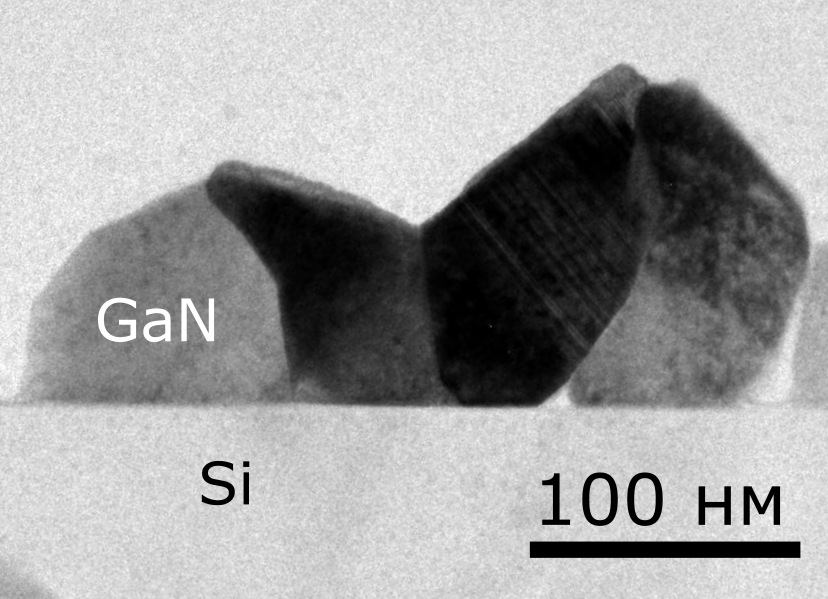
\includegraphics[height=7cm]{Image_18_1}}
			\subcaptionbox{\label{fig:Image_18_2}}{%
			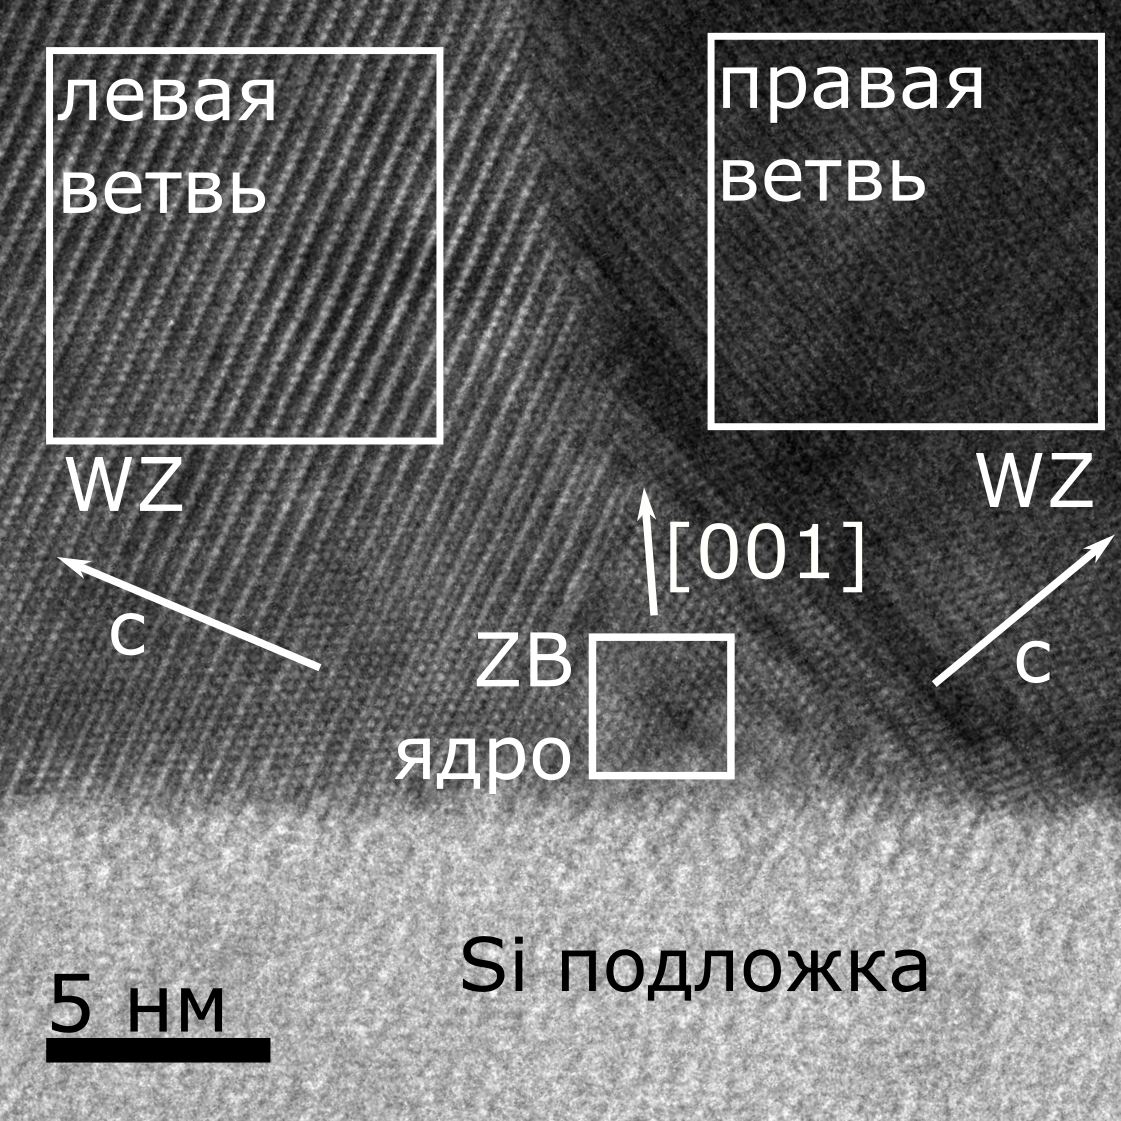
\includegraphics[height=7cm]{Image_18_2}}

		\subcaptionbox{\label{fig:Image_18_3}}{%
			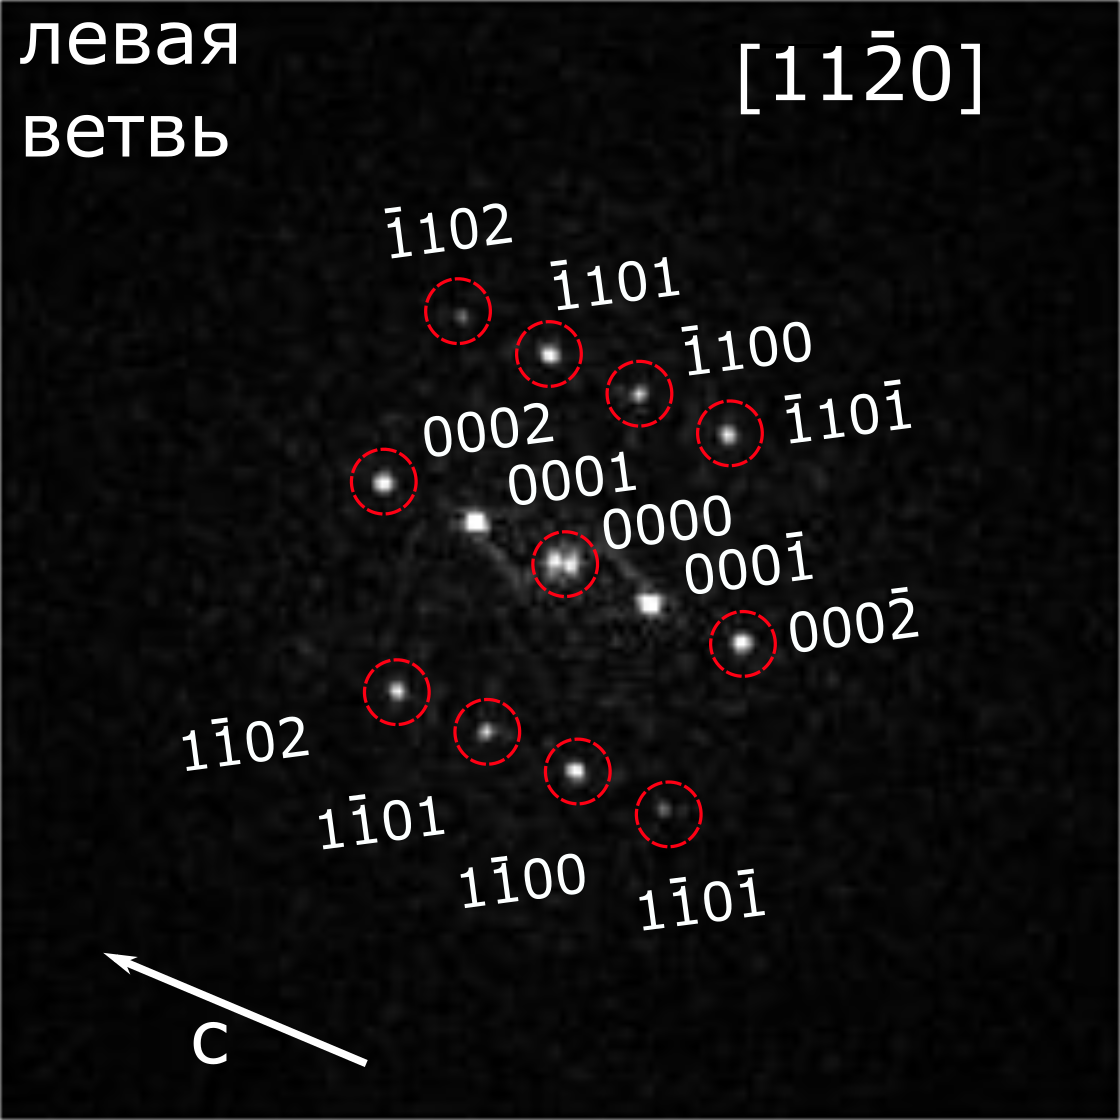
\includegraphics[width=0.31\linewidth]{Image_18_3}}
			\subcaptionbox{\label{fig:Image_18_4}}{%
				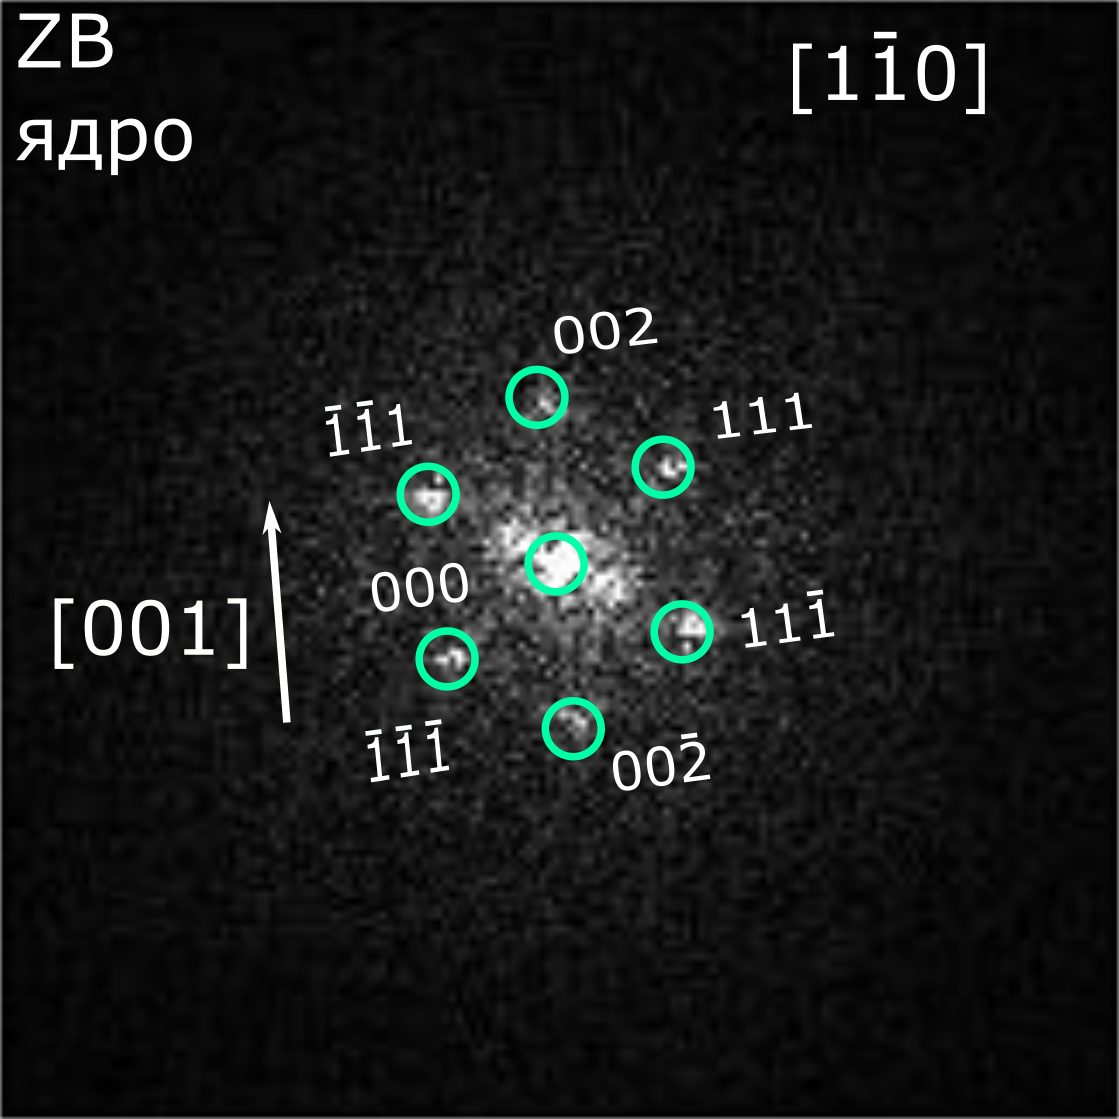
\includegraphics[width=0.31\linewidth]{Image_18_4}}
				\subcaptionbox{\label{fig:Image_18_5}}{%
				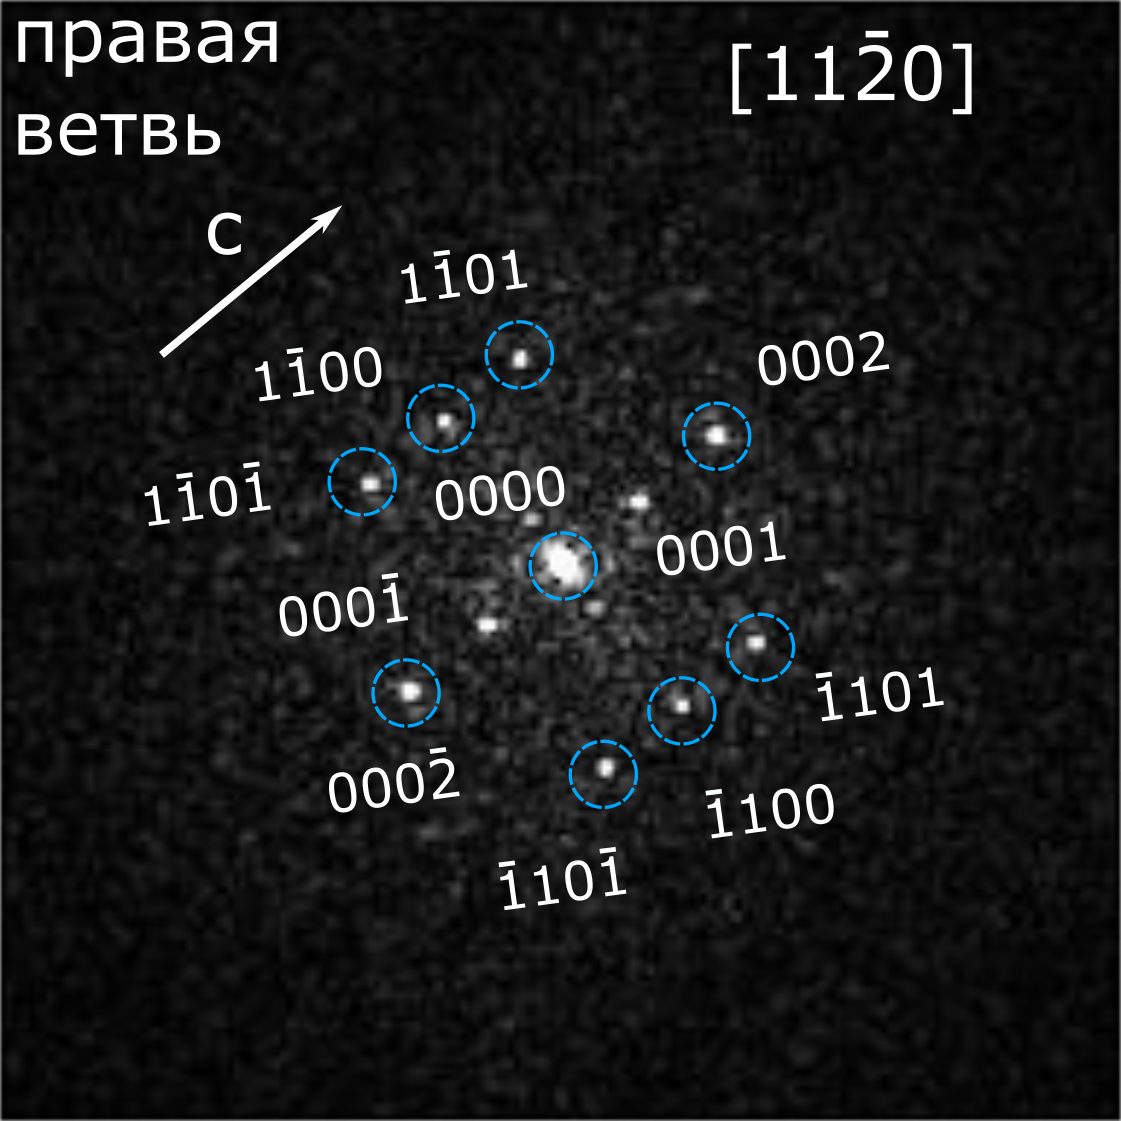
\includegraphics[width=0.31\linewidth]{Image_18_5}} } \caption{ПЭМ
				изображение наклонных ННК GaN с общим ядром~(а). Вид крупным планом
				ВРЭМ~(б) с соответствующими изображениями БПФ от отмеченных квадратами
		областей~(в\,--\,д)}\label{fig:Image_18} \end{figure}

\section{Исследование ФЛ триподов}\label{sec:ch3/sec5}

Для исследования ФЛ был выбран образец с высокой поверхностной плотностью
триподов \((\approx 20~\si{\micro\meter^{-2}})\). Измерения проводились при
температуре 10~\si{\kelvin} с возбуждением на длине волны 325~\si{\nano\meter}
непрерывным HeCd лазером. Типичный спектр ФЛ ансамбля нанотриподов GaN
(см.~рис.~\cref{fig:Image_19}) имеет три полосы: A (\(\approx
3,48\)~\si{\electronvolt}), B (\(\approx 3,43\)~\si{\electronvolt}) и C
(\(\approx 3,25\)~\si{\electronvolt)}.

Полоса A характерна для объёмного GaN со структурой WZ и соответствует
излучению вблизи края поглощения, что может быть связано со связанными на
нейтральном доноре экситонами \cite{Bolshakov2018, Richter2008, Agekyan2013}.

Полоса B может быть связана со структурными дефектами \cite{Calleja2000}, в
частности с наблюдаемыми дефектами упаковки в триподах
(см.~рис.~\cref{fig:Image_15_2}) \cite{Albrecht1997, Paskov2005}. В
Ni-каталитических ННК подобный пик вызван примесями Ni или наличием Ga вакансий
в структуре \cite{Yoo2006}.

Широкая полоса C может быть вызвана включениями ZB в GaN, так как ZB GaN при
низких температурах излучает вблизи края поглощения с энергией \(\approx
3,27\)~\si{\electronvolt} \cite{Jacobs2007}.

\begin{figure}[ht] \centerfloat{
		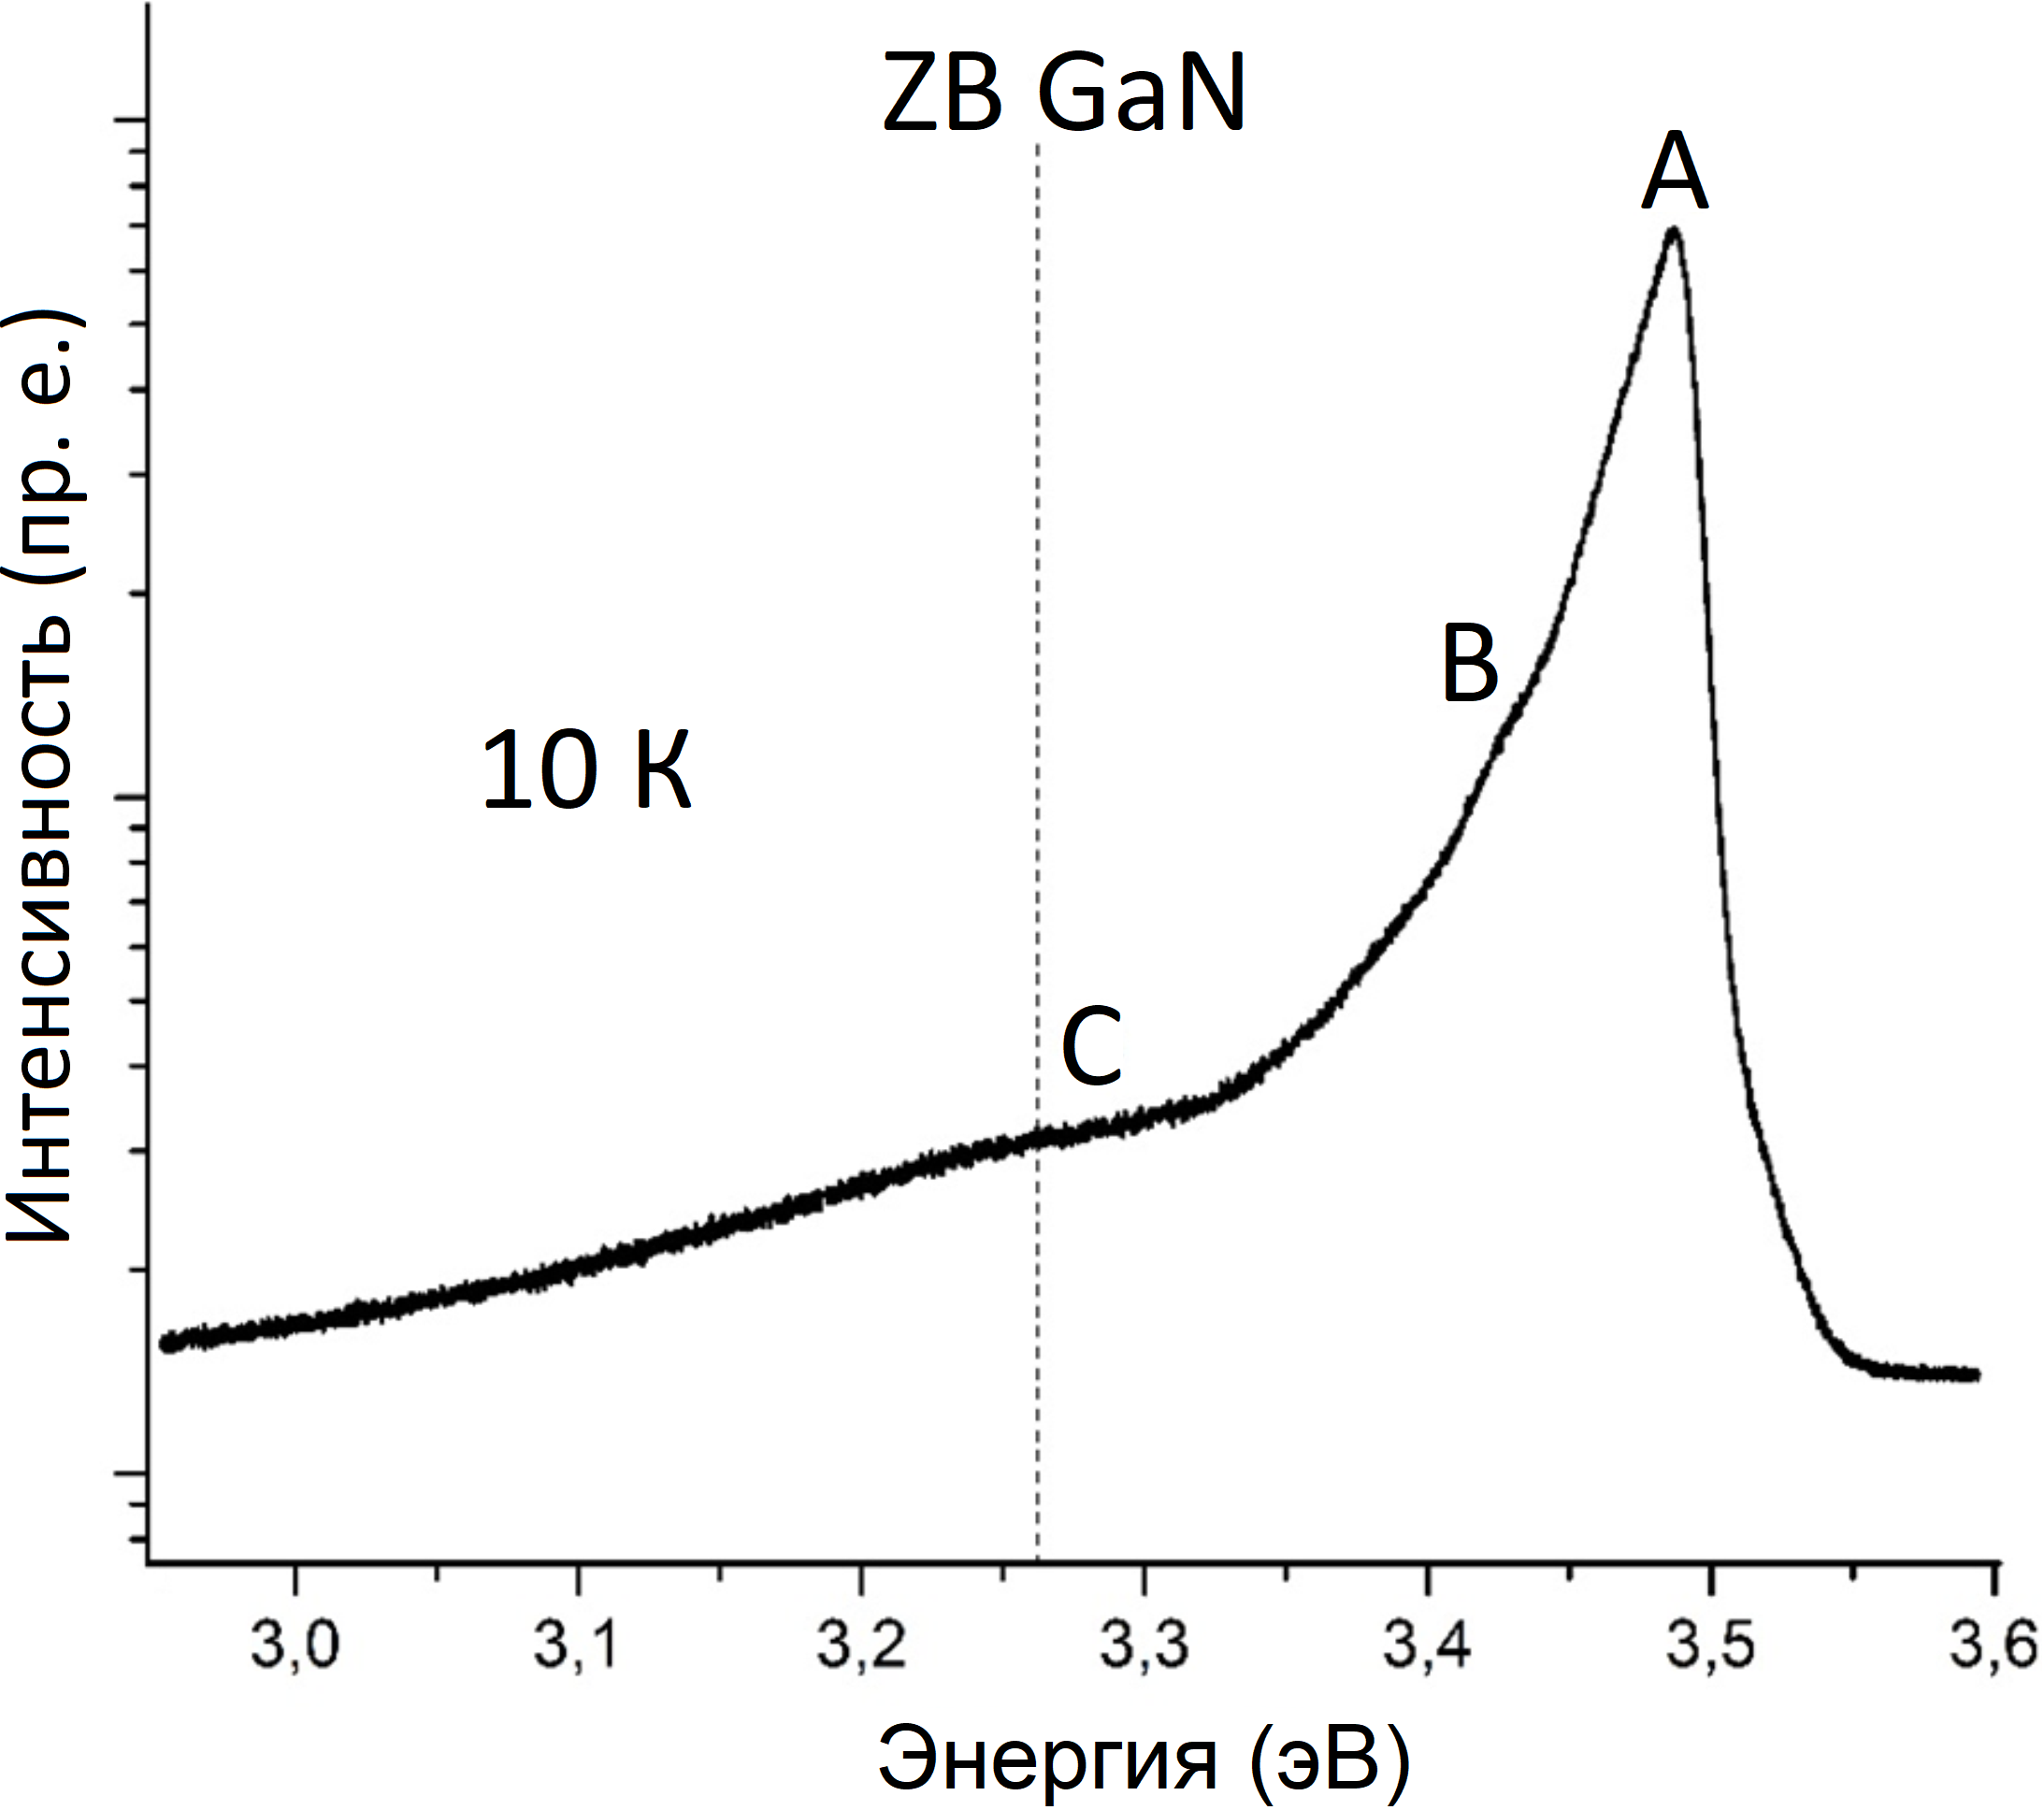
\includegraphics[width=0.5\linewidth]{Image_19} } \legend{Морфология
		поверхности образца изображена на~рисунке~\cref{fig:Image_25_1}, спектр
		снят при температуре 10~\si{\kelvin}} \caption{Низкотемпературный спектр ФЛ
		массива эпитаксиальных триподов GaN с высокой поверхностной
плотностью}\label{fig:Image_19} \end{figure}

\section{Влияние ростовых условий на морфологию
наноструктур}\label{sec:ch3/sec6}

\subsection{Влияние эквивалентной толщины затравочных
капель}\label{subsec:ch3/sec6/sub1}

Наноструктуры для анализа влияния эквивалентной толщины затравочных капель на
морфологию были синтезированы наноструктуры при следующих условиях роста: ЭДП
Ga \(1 \cdot 10^{-8}\)~\si{\torr}, расход азота
0,4~\si{\centi\meter^3\per\minute} и мощность плазменного источника
500~\si{\watt}.

Из сравнения образцов с нитридированными каплями различной эквивалентной
толщины (см.~рис.~\cref{fig:Image_20}) видно, что в исследуемом диапазоне
увеличение количества предварительно осаждённого Ga повышает плотность
затравочных островков GaN, но слабо влияет на их латеральный размер и
морфологию.

\begin{figure}[ht] \centerfloat{ \subcaptionbox{\label{fig:Image_20_1}}{%
			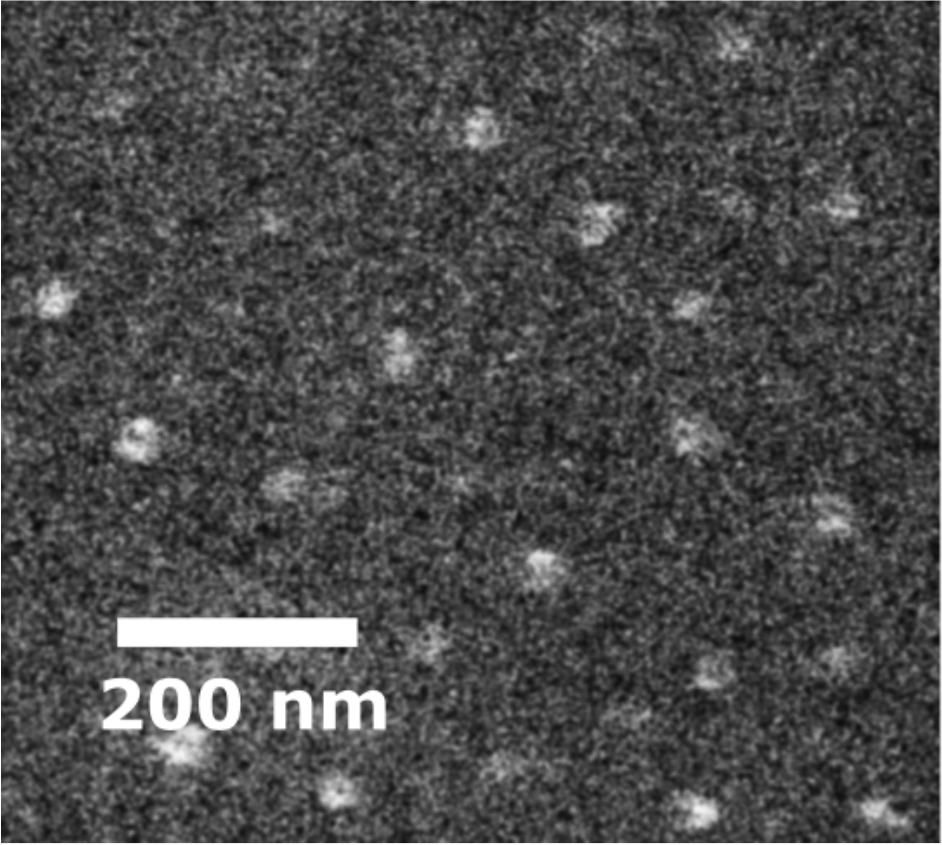
\includegraphics[width=0.25\linewidth]{Image_20_1}}
			\subcaptionbox{\label{fig:Image_20_2}}{%
			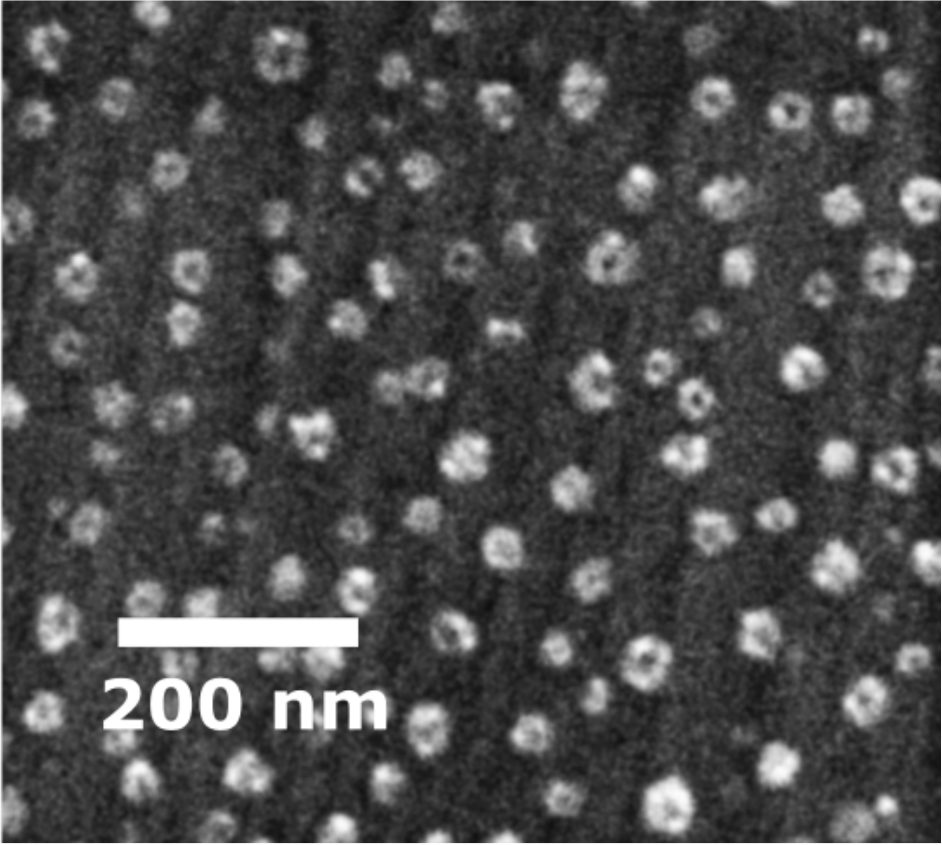
\includegraphics[width=0.25\linewidth]{Image_20_2}} }
			\legend{Эквивалентная толщиной капель Ga 1,35~(а) и 2~монослоя~(б)}
			\caption{РЭМ изображения затравочных островков GaN, выращенных методом
				капельной эпитаксии с различной эквивалентной толщиной капель
		Ga}\label{fig:Image_20} \end{figure}

Затравка Ga с эквивалентной толщиной менее 1~монослоя образует поверхностную
реконструкцию (см.~подраздел~\cref{subsec:ch2/sec1/sub2}), поэтому после
нитридации ZB островки не образуются. Следовательно, формирование триподов
подавляется, образуются исключительно ННК (см.~рис.~\cref{fig:Image_21}).

\begin{figure}[ht] \centerfloat{ \subcaptionbox{\label{fig:Image_21_1}}{%
			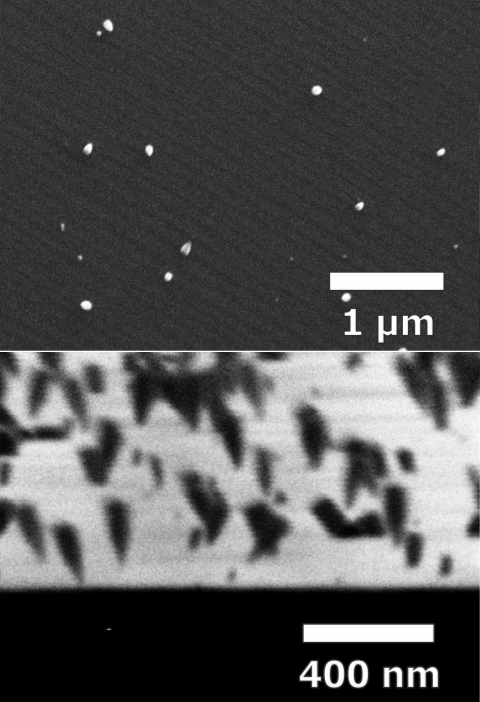
\includegraphics[width=0.25\linewidth]{Image_21_1}}
			\subcaptionbox{\label{fig:Image_21_2}}{%
			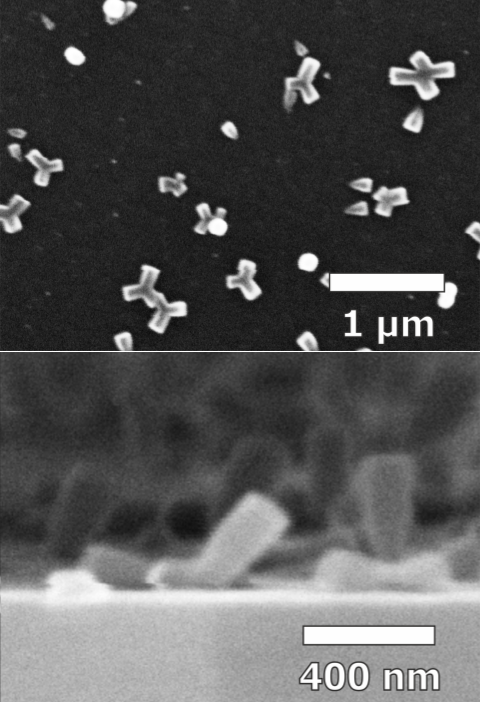
\includegraphics[width=0.25\linewidth]{Image_21_2}} }
			\legend{Эквивалентная толщина Ga 0,7~(а) и 2~монослоя~(б)} \caption{РЭМ
				изображения морфологии наноструктур GaN, синтезированных на затравочных
				островках различной эквивалентной толщины}\label{fig:Image_21}
			\end{figure}

Увеличение эквивалентной толщины затравки в диапазоне 0,7--1,4~монослоя
приводит к увеличению поверхностной плотности затравочных островков, а вместе с
тем увеличивает плотность и эквивалентную толщину синтезированных нанотриподов
(см.~рис.~\cref{fig:Image_22}).

\begin{figure}[ht] \centerfloat{ \subcaptionbox{\label{fig:Image_22_1}}{%
			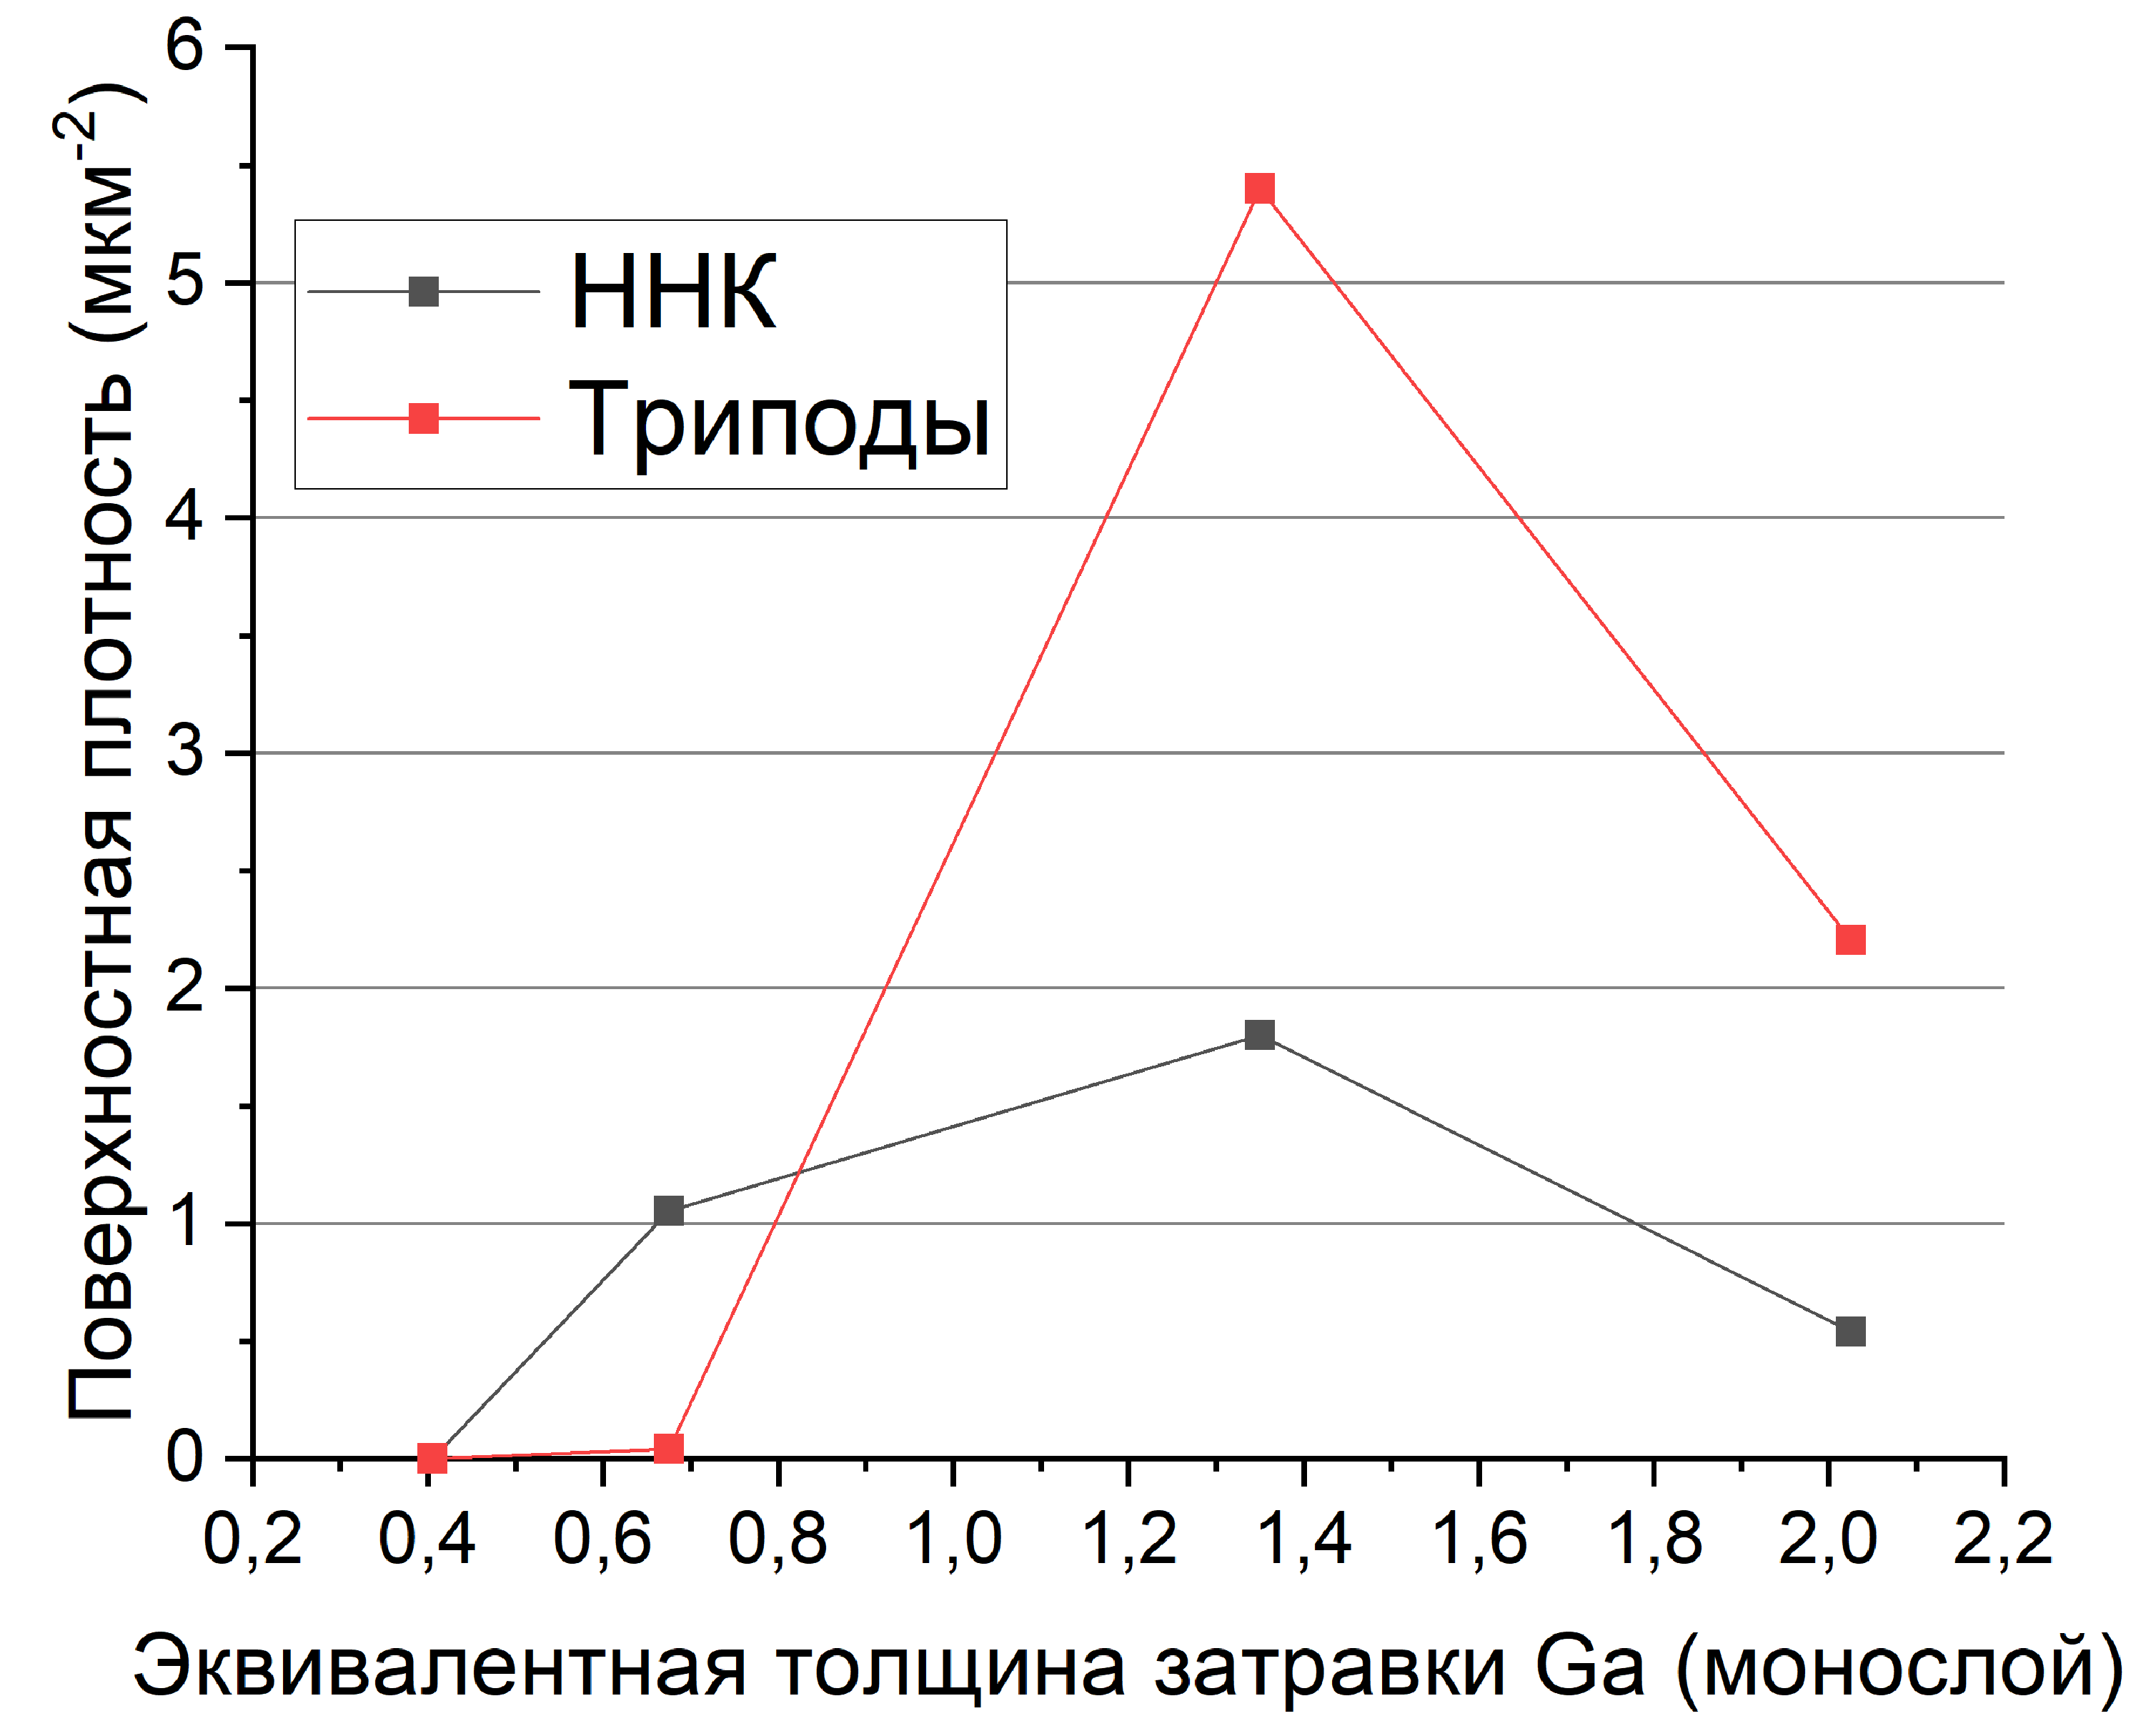
\includegraphics[width=0.48\linewidth]{Image_22_1}}
			\subcaptionbox{\label{fig:Image_22_2}}{%
			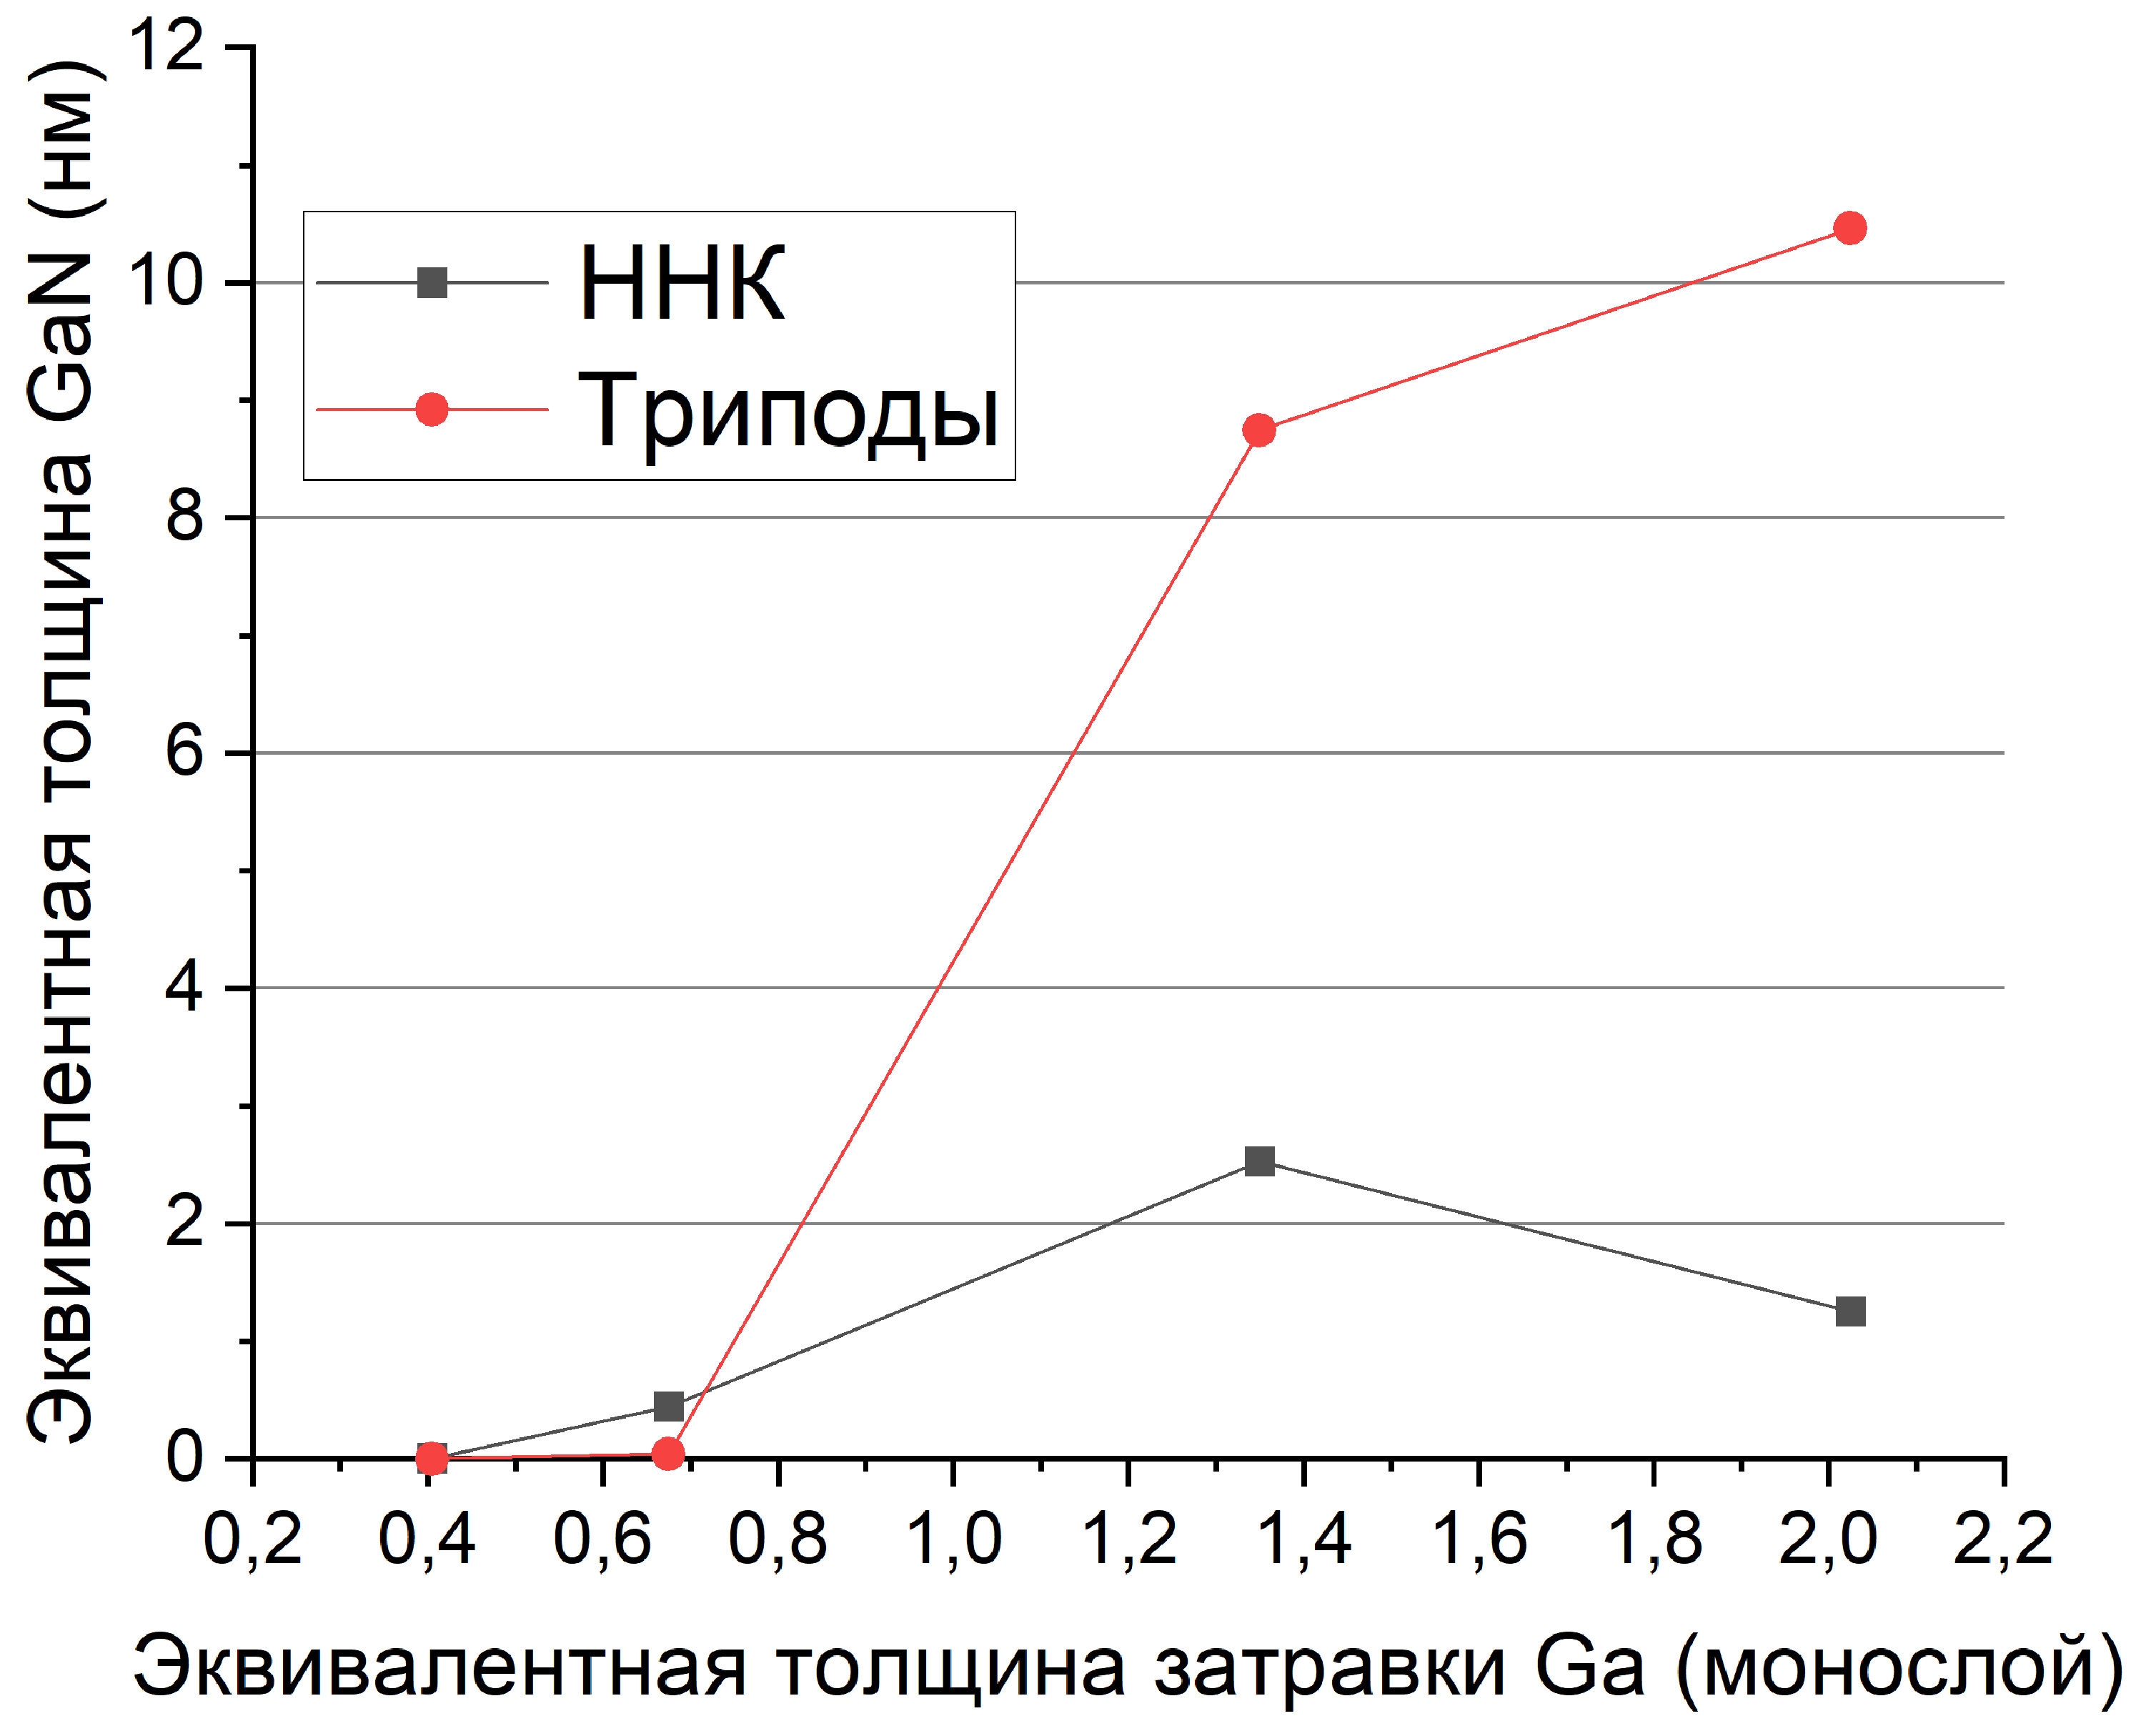
\includegraphics[width=0.48\linewidth]{Image_22_2}} }
			\caption{Зависимости эквивалентной толщины~(а) синтезированного материала
				и поверхностной плотности~(б) массива наноструктур GaN от эквивалентной
				толщины затравочных островков}\label{fig:Image_22} \end{figure}

Эквивалентная толщина синтезированного массива насыщается с дальнейшим
увеличением эквивалентной толщины затравочных капель. Высокая поверхностная
плотность затравочных наноостровков, служащих центрами зародышеобразования,
приводит к слиянию наноструктур массива при дальнейшем росте. Это объясняет
внезапное падение поверхностных плотностей массивов при толщине затравочного
слоя более 1,7~монослоя (см.~рис.~\cref{fig:Image_22}). Использование
затравочных капель с эквивалентной толщиной более 2,4~монослоя приводит к
формированию двумерного слоя GaN из сросшихся островков.

\subsection{Влияние соотношения молекулярных потоков
V/III}\label{subsec:ch3/sec6/sub2}

Для изучения влияния соотношения V/III на формирование триподов проведена
ростовая серия с образцами, синтезированными при различных ЭДП Ga
(см.~рис.~\cref{fig:Image_23}).

\begin{figure}[ht] \centerfloat{ \subcaptionbox{\label{fig:Image_23_1}}{%
			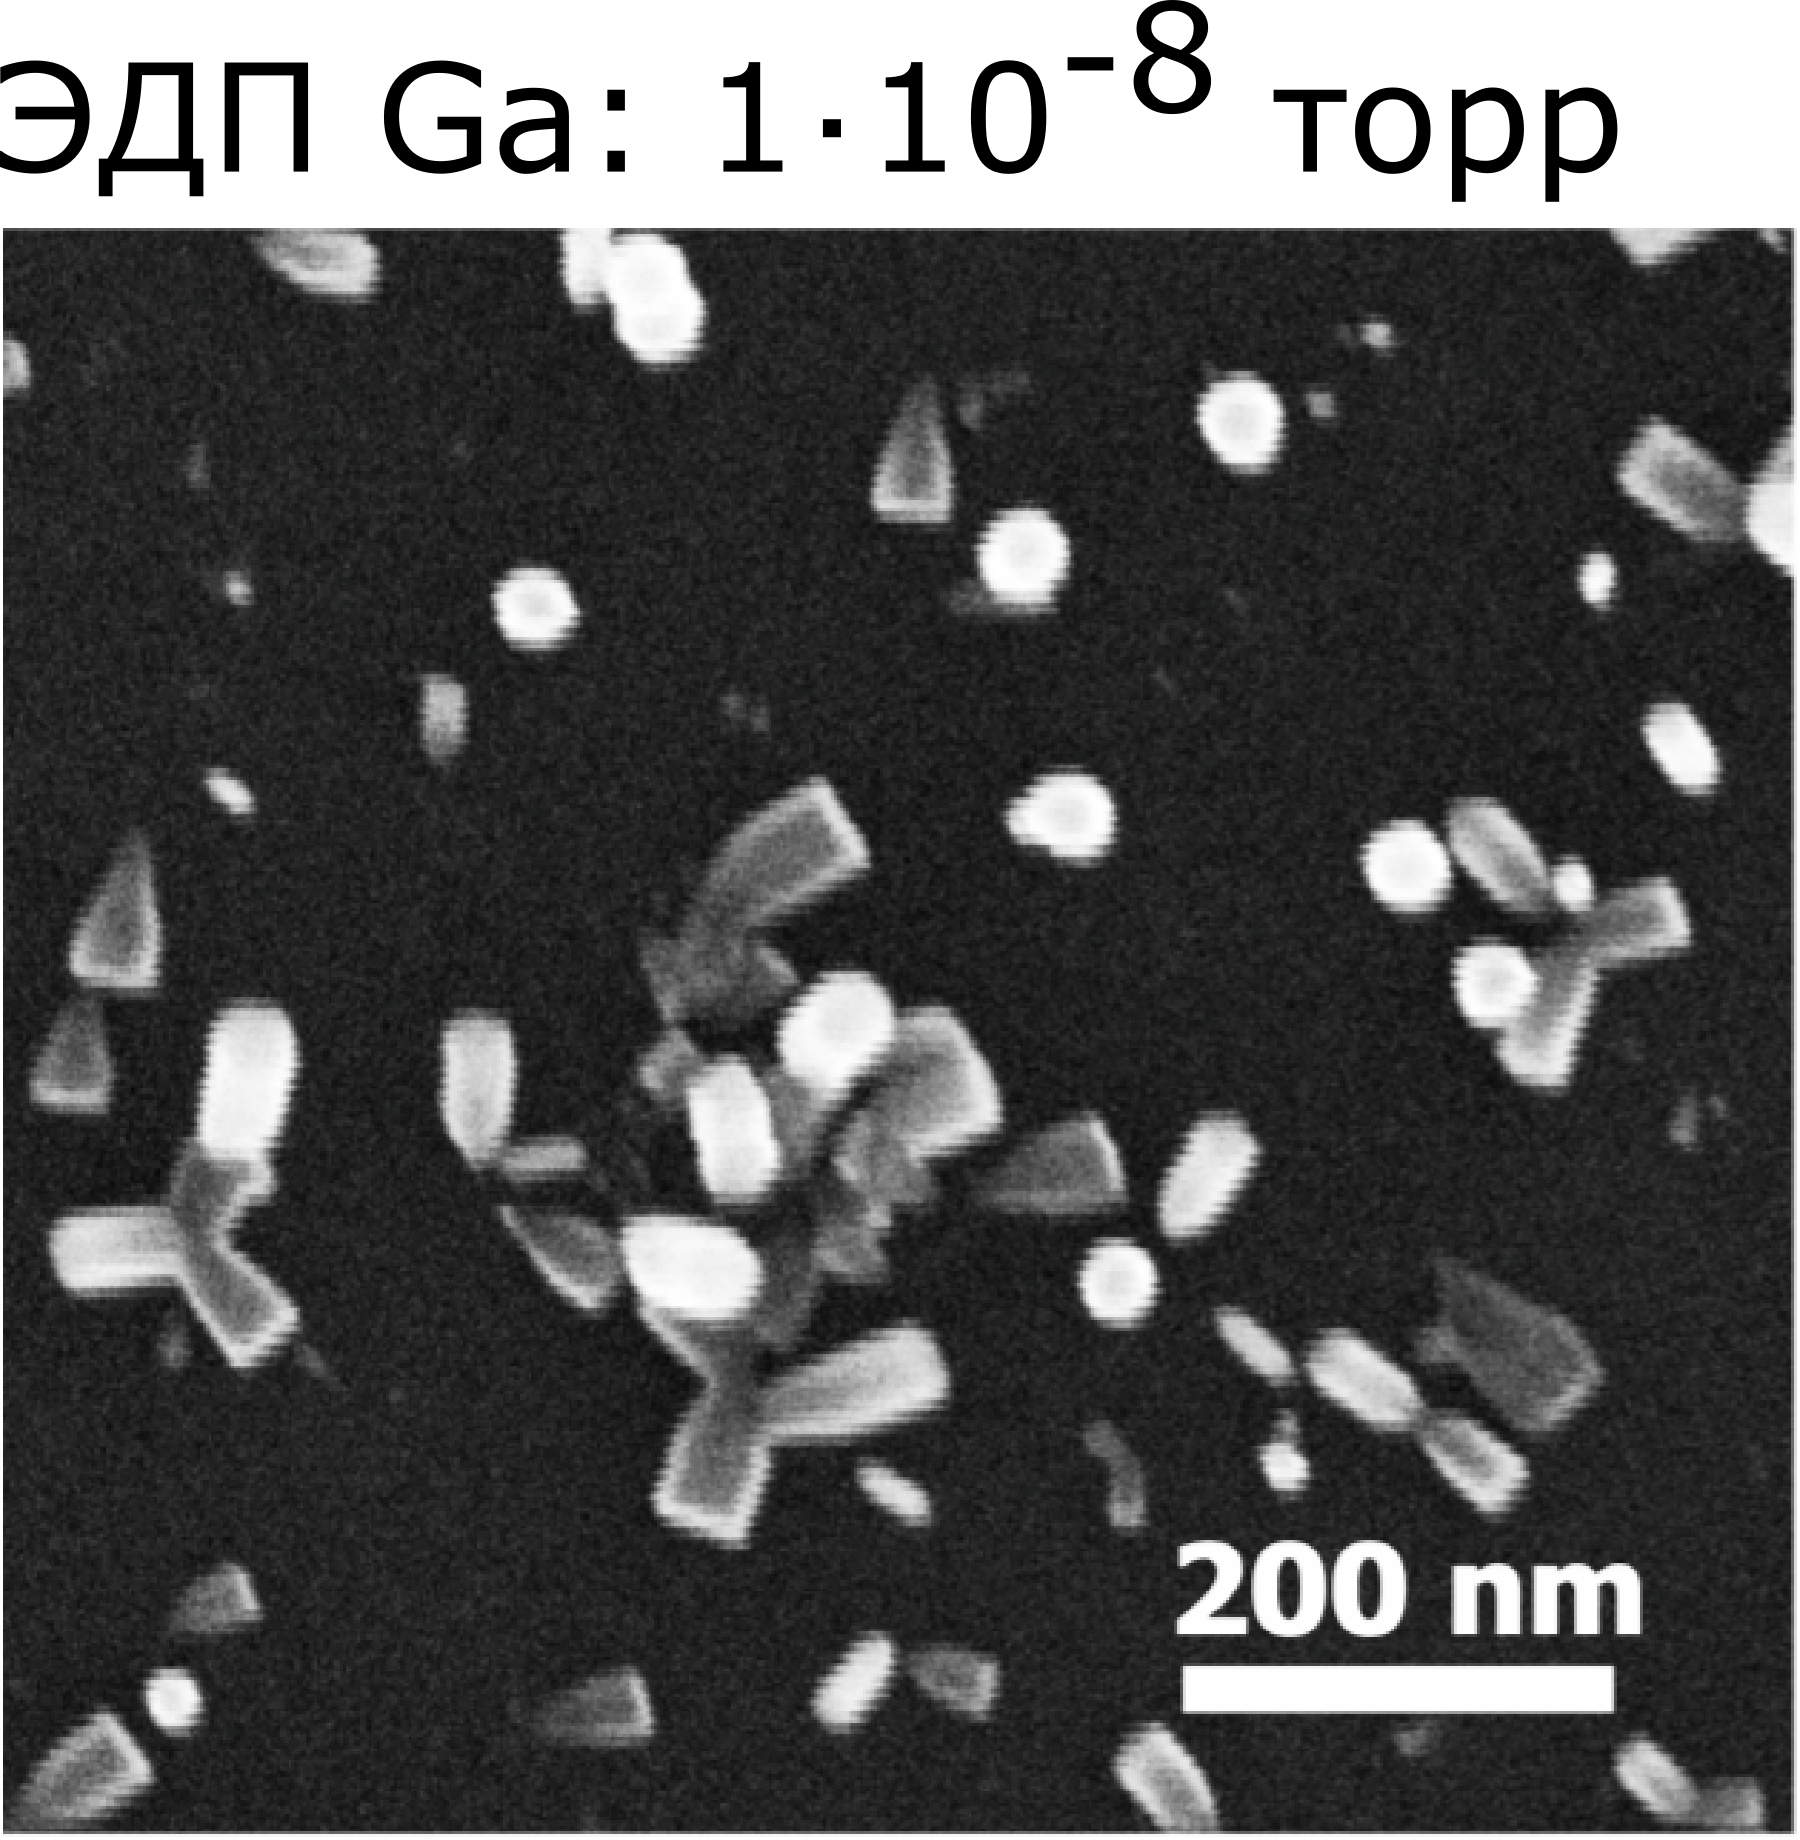
\includegraphics[width=0.25\linewidth]{Image_23_1}}
			\subcaptionbox{\label{fig:Image_23_2}}{%
				\includegraphics[width=0.25\linewidth]{Image_23_2}}
				\subcaptionbox{\label{fig:Image_23_3}}{%
				\includegraphics[width=0.25\linewidth]{Image_23_3}} } \legend{ЭДП Ga
				\(1 \cdot 10^{-8}\)~(а), \(1,5 \cdot 10^{-8}\)~(б), \(2 \cdot
				10^{-8}\)~\si{\torr}~(в)} \caption{РЭМ изображения наноструктур GaN,
		выращенных при различных ЭДП Ga}\label{fig:Image_23} \end{figure}

Согласно работе \cite{Voulot1998}, расход азота или ВЧ мощность влияет не
только на ЭДП активированного азота, но и на соотношение в нем атомов, молекул
и ионов \cite{Blant2000}, поэтому корреляции между расходом азота и потоком
активированного азота нелинейная. По этой причине параметры источника плазмы
сохранялись постоянными (расход азота 1~\si{\centi\meter^3\per\minute}, ВЧ
мощность 500~\si{\watt}).

Увеличение ЭДП Ga в исследуемом диапазоне уменьшает скорость роста вертикальных
и наклонённых ННК, снижает аспектное отношение ННК и триподов (длина/толщина)
(см.~рис.~\cref{fig:Image_24_1},~ \cref{fig:Image_24_2}), повышает сужение ННК
у основания. Поверхность подложки в основном занята триподами при ЭДП Ga \(1,5
\cdot 10^{-8}\)~\si{\torr}, а при потоке выше и ниже этого значения на
поверхности доминируют ННК (см.~рис.~\cref{fig:Image_24_1}).

\begin{figure}[ht] \centerfloat{ \subcaptionbox{\label{fig:Image_24_1_1}}{%
			\includegraphics[width=0.48\linewidth]{Image_24_1_1}}
			\subcaptionbox{\label{fig:Image_24_1_2}}{%
			\includegraphics[width=0.48\linewidth]{Image_24_1_2}} }
			\caption{Зависимости поверхностной плотности~(а) и эквивалентной толщины
			осаждённого материала~(б) наноструктур GaN от ЭДП
		Ga}\label{fig:Image_24_1} \end{figure}

\begin{figure}[ht] \centerfloat{
\includegraphics[width=0.6\linewidth]{Image_24_2} } \caption{Зависимости
линейных размеров наноструктур GaN от ЭДП Ga}\label{fig:Image_24_2}
\end{figure}

Эквивалентная толщина осаждаемого материала (см.~рис.~\cref{fig:Image_24_1_2})
не пропорциональна ЭДП Ga~--- увеличение поверхностной плотности
(см.~рис.~\cref{fig:Image_24_1_1}) компенсируется уменьшением среднего
поперечного размера наноструктур (см.~рис.~\cref{fig:Image_24_2}).

\subsection{Влияние ростовой температуры подложки}\label{subsec:ch3/sec6/sub3}

Наноструктуры формировались в узком температурном диапазоне с 690 до
710~\si{\degreeCelsius} (см.~рис.~\cref{fig:Image_25}). При температуре роста
690~\si{\degreeCelsius} поверхностная плотность триподов становится настолько
высокой, что они срастаются и покрывают почти всю поверхность подложки
(см.~рис.~\cref{fig:Image_26_1_1}). Поверхностная плотность наноструктур быстро
падает с температурой. Формирование триподов полностью подавляется при
температурах выше 705~\si{\degreeCelsius}.

\begin{figure}[ht] \centerfloat{ \subcaptionbox{\label{fig:Image_25_1}}{%
			\includegraphics[width=0.25\linewidth]{Image_25_1}}
			\subcaptionbox{\label{fig:Image_25_2}}{%
				\includegraphics[width=0.25\linewidth]{Image_25_2}}
				\subcaptionbox{\label{fig:Image_25_3}}{%
				\includegraphics[width=0.25\linewidth]{Image_25_3}} } \legend{Ростовая
				температура: 690~\si{\degreeCelsius}~(а), 700~\si{\degreeCelsius}~(б),
				710~\si{\degreeCelsius}~(в)} \caption{РЭМ изображения (вид сверху и
				сбоку) морфологии наноструктур GaN, синтезированных при различных
		температурах подложки}\label{fig:Image_25} \end{figure}

\begin{figure}[ht] \centerfloat{ \subcaptionbox{\label{fig:Image_26_1_1}}{%
			\includegraphics[width=0.48\linewidth]{Image_26_1_1}}
			\subcaptionbox{\label{fig:Image_26_1_2}}{%
			\includegraphics[width=0.48\linewidth]{Image_26_1_2}} }
			\caption{Зависимости поверхностной плотности~(а) и эквивалентной
		толщины~(б) наноструктур GaN от температуры роста}\label{fig:Image_26_1}
	\end{figure}

Эквивалентная толщина синтезированного материала и поверхностная плотность
наноструктур уменьшаются на порядок с повышением температуры с 690 до
710~\si{\degreeCelsius} (см.~рис.~\cref{fig:Image_26_1}). При температуре
700~\si{\degreeCelsius} формируются наиболее длинные ННК и наиболее крупные
триподы (см.~рис.~\cref{fig:Image_26_2}). Повышение температуры роста
увеличивает длину свободного пробега адатомов, что при 700~\si{\degreeCelsius}
приводит к увеличению аксиальной скорости роста. Можно предположить, что
снижение скорости роста наноструктур при дальнейшем повышении температуры
вызвано доминированием десорбции адатомов (см.~рис.~\cref{fig:Image_26_2}).

\begin{figure}[ht] \centerfloat{
	\includegraphics[width=0.6\linewidth]{Image_26_2} } \caption{Зависимости
линейных размеров наноструктур GaN от температуры роста}\label{fig:Image_26_2}
\end{figure}

Основание ННК имеет сужение к подложке. Угол вершины конуса основания ННК
(см.~рис.~\cref{fig:Image_25}) зависит от температуры и времени роста и лежит в
диапазоне от 20{\textdegree} до 42{\textdegree} (\(20\si{\degree} \pm
4\si{\degree}\) при температуре роста 710~\si{\degreeCelsius} и
\(42\si{\degree} \pm 2\si{\degree}\) при температуре роста
700~\si{\degreeCelsius}) \cite{Bolshakov2014}. Морфология ННК может зависеть от
положения подложки относительно источника \cite{Galopin2011}, поскольку оно
влияет на соотношение между молекулярными потоками, попадающими на боковые
стенки и верхнюю грань, таким образом оказывая влияние на длину свободного
пробега до встраивания адатомов Ga на боковых стенках. Это объясняет
зависимость от температуры: если источник азота расположен ортогонально
подложке~--- формируются GaN ННК с однородным по длине диаметром, а если под
острым (как в МПЭ установке Veeco GEN III)~--- ННК с утолщением.

\section{Основные результаты}\label{sec:ch3/sec7}

Продемонстрирован эпитаксиальный синтез методом ПА-МПЭ наноструктур и в форме
GaN ННК и триподов на Si(111) подложке с предварительным формированием
затравочных наноостровков GaN. После нитридации наноостровки приобретают
кольцеобразную форму. Данные островки имеют ZB структуру и впоследствии
находятся в основе триподов и наклонённых ННК.

Поверхностная плотность, размер и аспектное отношение структур можно
контролировать температурой роста, потоком III группы и эквивалентной толщиной
затравочного слоя. Нуклеация триподов может быть полностью подавлена путем
уменьшения эквивалентной толщины затравки Ga и повышения температуры роста выше
710~\si{\degreeCelsius}.

Направление ветвей соответствует кристаллографическому направлению
<\(0001\)>\textsubscript{GaN} с преимущественной ориентацией вдоль направлений
<\(1\overline{1}0\)>\textsubscript{Si}, <\(11\overline{2}\)>\textsubscript{Si}
и \(<12\overline{3}>\)\textsubscript{Si}. Плоскость
\((11\overline{2}1)\)\textsubscript{GaN} триподов имеет эпитаксиальное
отношение с параллельной плоскостью подложки (111)\textsubscript{Si}.

Спектр ФЛ от массив нанотриподов с включениями политипа ZB имеет три полосы:
интенсивную полосу, характерную для объёмного WZ GaN (\(\approx
3,48\)~\si{\electronvolt}), полосу, характерную для GaN с дефектами упаковки
(\(\approx 3,43\)~\si{\electronvolt}) и полосу, характерную для ZB GaN
(\(\approx 3,25\)~\si{\electronvolt}).

\FloatBarrier
           % Глава 3
\chapter{Эпитаксиальные наночастицы GaAs}\label{ch:ch4}

GaAs~--- третий по масштабам использования в полупроводниковой промышленности
материал после кремния и германия. В последнее десятилетие разработано
несколько важных приложений на основе синтезированных на Si наноструктур GaAs:
солнечные элементы \cite{Chu2014}, активный слой для оптоэлектронных устройств
\cite{Bietti2009}, структура металл\,--\,оксид\,--\,полупроводник
\cite{Zhao2009}, однофотонный излучатель \cite{Sanguinetti2015}.

В этой главе излагается результат исследований формирования методом МПЭ и
оптических свойств эпитаксиальных наночастиц GaAs на подложках Si(111) без
поверхностного оксида. Показано, что GaAs может образовывать огранённые
наночастицы, окружённые сплошным слоем сросшихся островков GaAs. Исследовано
влияние условий синтеза на морфологию наноструктур.

\section{Постановка эксперимента}\label{sec:ch4/sec1}

Наноструктуры GaAs синтезированы на установке МПЭ Veeco GEN III на подложках
Si(111). Перед загрузкой в установку подложки химически обрабатывались
последовательным кипячением в растворах CCl\textsubscript{4}, изопропанола и
растворе
NH\textsubscript{4}OH:H\textsubscript{2}O\textsubscript{2}:H\textsubscript{2}O
в соотношении 1:1:3, естественный поверхностный оксид удалялся погружением в
1:10 раствор HF:H\textsubscript{2}O с последующим промыванием в
деионизированной воде. После загрузки в установку подложки дегазировали в
промежуточной камере при температуре 400~\si{\degreeCelsius}. В ростовой камере
подложка нагревалась до температуры роста без предварительного
высокотемпературного отжига.

Рост начинался одновременной подачей молекулярных потоков Ga и
As\textsubscript{4}. Во время роста всех исследуемых образцов поток Ga
поддерживался постоянным и соответствовал планарной скорости роста
GaAs/GaAs(001) равной 0,4~\si{\micro\metre\per\hour} в избытке As. При
обсуждении поток As\textsubscript{4} в работе используются относительные
единицы, за единицу которых взят «стехиометрический» поток~--- абсолютный поток
As\textsubscript{4} при котором в сочетании с потоком Ga, который соответствует
планарной скорости роста GaAs/GaAs(001) равной 0,4~\si{\micro\metre\per\hour} в
избытке As, достигается стехиометрическое отношение адатомов на поверхности
GaAs, определяемое по фазовому переходу от As-обогащённой реконструкции
GaAs\((001)4\)\(\times\)\(2\) к Ga-обогащённой GaAs\((001)2\)\(\times\)\(4\)
при температуре подложки 550~\si{\degreeCelsius} во время роста планарного
GaAs/GaAs(001). Данный переход наблюдается при отношении ЭДП
As\textsubscript{4}/Ga \(\approx 12\). Данные условия роста приводят к
образованию одиночных наночастиц GaAs, окружённых шероховатым сплошным слоем.

Морфология синтезированных наногетероструктур изучена методом PЭМ (Zeiss SUPRA
25) и АСМ (Bruker Bioscope Catalyst SPM). Изображения АСМ обработаны в
программе Gwyddion. Спектры КРС и ФЛ получены при комнатной температуре
(300~\si{\kelvin}), используя лазерное возбуждение с длиной волны
532~\si{\nano\metre} на спектрометре Horiba LabRam HR800. Спектрометр совмещён
с пьезодвигателем, позволяющим проводить измерения в геометрии обратного
рассеяния с пространственным разрешением менее 0,5~\si{\micro\metre}, и
оптическим конфокальным микроскопом Olympus IX71 с объективом Olympus Plan N
100\(\times\)/0,95~NA.

\section{Влияние ростовых параметров на морфологию наночастиц}\label{sec:ch4/sec2}

Для исследования влияния условий роста на морфологию наночастиц GaAs
синтезированы образцы при различных ЭДП As и ростовых температурах подложки с
сохранением постоянного потока Ga. Влияние изменения соотношения молекулярных
потоков As/Ga было изучено на основе образцов, выращенных при температуре
подложки 550~\si{\degreeCelsius}, потоке As в 2, 4 и 6~отн.~ед.

На поверхности подложки вокруг эпитаксиальных наночастиц GaAs отсутствует
синтезированный материал, на РЭМ изображениях эта область имеет тёмный контраст
(см.~рис.~\cref{fig:Image_31}). Можно предположить, что наночастицы могут
зарождаться на неоднородностях поверхности подложки: на островках
SiO\textsubscript{x}, образующихся до загрузки подложек в установку МПЭ
\cite{Miura1996, Ogawa1996}, или шероховатостях из-за неоднородного окисления
подложки и последующего травления в HF \cite{Neuwald1992, Jakob1991}. Адатомы
Ga накапливается на этих участках с последующим формированием наночастиц GaAs в
режиме ПЖК \cite{Dubrovskii2012a}, а обычный трёхмерный рост в режиме
пар\,--\,кристалл с высокой поверхностной плотностью зарождения происходит на
свободной поверхности Si(111).

\begin{figure}[ht] \centerfloat{ \subcaptionbox{\label{fig:Image_31_1}}{%
			\includegraphics[width=0.27\linewidth]{Image_31_1}}
			\subcaptionbox{\label{fig:Image_31_2}}{%
				\includegraphics[width=0.27\linewidth]{Image_31_2}}
				\subcaptionbox{\label{fig:Image_31_3}}{%
				\includegraphics[width=0.27\linewidth]{Image_31_3}} } \legend{Поток As:
				2 (а), 4 (б) и 6~отн.~ед (в) (температура роста
				550~\si{\degreeCelsius})} \caption{РЭМ изображения наноструктур GaAs,
				синтезированных при различных потоках As}\label{fig:Image_31}
			\end{figure}

Результаты анализа влияния соотношения молекулярных потоков As/Ga на морфологию
наночастиц представлены на рисунках~\cref{fig:tab_2} и ~\cref{fig:tab_2_3}. При
низком соотношении потоков As/Ga (поток As 2~отн.~ед.) формируется самая низкая
поверхностная плотность массива наночастиц, наибольший латеральный размер и
высота наночастиц. Увеличение соотношения потоков As/Ga (увеличение потока As с
2 до 4~отн.~ед.) приводит к трёхкратному увеличению поверхностной плотности
массива наночастиц и резкому уменьшению их латерального размера (с \(\approx
1900\)~\si{\nano\metre} до \(\approx 250\)~\si{\nano\metre}). Дальнейшее
увеличение соотношения потоков As/Ga (увеличение потока As с 4 до 6~отн.~ед.)
оказывает слабое влияние на морфологию наночастиц и сплошного слоя, что
указывает на переход к режиму ограничения скорости роста потоком Ga.

\begin{figure}[ht] \centerfloat{ \subcaptionbox{\label{fig:tab_2_1}}{%
			\includegraphics[width=0.48\linewidth]{tab_2_1}}
			\subcaptionbox{\label{fig:tab_2_2}}{%
			\includegraphics[width=0.48\linewidth]{tab_2_2}} } \legend{Наноструктуры
			GaAs синтезированы при температуре подложки 550~\si{\degreeCelsius}}
			\caption{Зависимости поверхностной плотности массива~(а) и линейных
				размеров наночастиц~(б)  от соотношения потоков As/Ga}\label{fig:tab_2}
			\end{figure}

\begin{figure}[ht] \centerfloat{
		\includegraphics[width=0.48\linewidth]{tab_2_3} } \legend{Наноструктуры
		GaAs синтезированы при температуре подложки 550~\si{\degreeCelsius}}
		\caption{Зависимость толщины сплошного слоя от соотношения потоков
	As/Ga}\label{fig:tab_2_3} \end{figure}

Влияние соотношения потоков As/Ga на морфологию наночастиц вызвано подавлением
диффузии адатомов Ga адатомами V группы. Снижение потока As ниже 2~отн.~ед.
может привести к накоплению капель Ga, а увеличение~--- подавить диффузию
частиц Ga, что увеличивает поверхностную плотность наночастиц и способствует
росту сплошного слоя.

Другой контролируемый ростовой параметр~--- температура подложки. Для
исследования его влияния была синтезирована серия образцов при температуре
роста от 550 до 630~\si{\degreeCelsius} и потоке As в 4~отн.~ед.
(см.~рис.~\cref{fig:Image_32}).

\begin{figure}[ht] \centerfloat{ \subcaptionbox{\label{fig:Image_32_1}}{%
			\includegraphics[width=0.27\linewidth]{Image_32_1}}
			\subcaptionbox{\label{fig:Image_32_2}}{%
				\includegraphics[width=0.27\linewidth]{Image_32_2}}
				\subcaptionbox{\label{fig:Image_32_3}}{%
				\includegraphics[width=0.27\linewidth]{Image_32_3}} }
				\legend{Температура роста: 550~\si{\degreeCelsius}~(а),
					580~\si{\degreeCelsius}~(б), 630~\si{\degreeCelsius}~(в) (поток As
					4~отн.~ед.)} \caption{РЭМ изображения наноструктур GaAs на Si,
			синтезированных при различных температурах}\label{fig:Image_32}
		\end{figure}

Сравнение РЭМ изображений поверхности образцов указывает на схожесть влияния
повышения температуры и снижения соотношения потоков As/Ga
(см.~рис.~\cref{fig:tab_3} и~\cref{fig:tab_3_3}): повышение температуры
стимулирует десорбцию As. Это предположение подтверждается накоплением капель
Ga на поверхности при дальнейшем повышении температуры
(см.~рис.~\cref{fig:Image_32_3}).

\begin{figure}[ht] \centerfloat{ \subcaptionbox{\label{fig:tab_3_1}}{%
			\includegraphics[width=0.48\linewidth]{tab_3_1}}
			\subcaptionbox{\label{fig:tab_3_2}}{%
			\includegraphics[width=0.48\linewidth]{tab_3_2}} } \legend{Наноструктуры
			GaAs синтезированы при при потоке As в 4~отн.~ед.} \caption{Зависимости
			поверхностной плотности массива~(а) и линейных размеров наночастиц~(б) от
	температуры роста}\label{fig:tab_3} \end{figure}

\begin{figure}[ht] \centerfloat{
		\includegraphics[width=0.48\linewidth]{tab_3_3} } \legend{Наноструктуры
		GaAs синтезированы при при потоке As в 4~отн.~ед.} \caption{Зависимость
		толщины сплошного слоя от температуры роста}\label{fig:tab_3_3}
	\end{figure}

Таким образом, изменение соотношения потоков As/Ga и температуры роста может
использоваться для контроля размеров и плотности наночастиц GaAs.

\section{Изменение морфологии в процессе роста}\label{sec:ch4/sec3}

Для изучения изменения морфологии наночастиц во время роста выращены два
образца при одинаковых условиях синтеза в течение 10 и 30~\si{\minute}.
Температура роста образцов~--- 550°C, поток As в 4~отн.~ед. Площадь области
свободной от кристаллизованного GaAs, окружающей наночастицы, и поверхностная
плотность наночастиц значительно уменьшается (с 0,08 до
0,007~\si{\per\micro\metre\squared}) во время роста
(см.~рис.~\cref{fig:Image_33}).

\begin{figure}[ht] \centerfloat{ \subcaptionbox{\label{fig:Image_33_1}}{%
			\includegraphics[width=0.4\linewidth]{Image_33_1}}
			\subcaptionbox{\label{fig:Image_33_2}}{%
			\includegraphics[width=0.4\linewidth]{Image_33_2}} } \legend{Температура
			роста образцов 550~\si{\degreeCelsius}, поток As в 4~отн.~ед.}
			\caption{РЭМ изображения эпитаксиальных наночастиц GaAs на поверхности
				Si, выращенных в течение 10~(а) и
		30~\si{\minute}~(б)}\label{fig:Image_33} \end{figure}

Сплошной слой образован слиянием наноостровков (см.~рис.~\cref{fig:Image_33},
\cref{fig:Image_34}) с гранями, параллельными поверхности подложки
(111)\textsubscript{Si}. Высота и латеральный размер наночастиц, выращенных в
течении 30~\si{\minute}, остаётся близкой к высоте наночастиц, синтезированных
в течение 10~\si{\minute}. При этом толщина сплошного слоя увеличилась с
\(\approx 50\) до \(\approx 200\)~\si{\nano\metre}
(см.~рис.~\cref{fig:Image_34}).

\begin{figure}[ht] \centerfloat{ \subcaptionbox{\label{fig:Image_34_1}}{%
			\includegraphics[width=0.4\linewidth]{Image_34_1}}
			\subcaptionbox{\label{fig:Image_34_2}}{%
			\includegraphics[width=0.4\linewidth]{Image_34_2}} } \legend{Температура
			роста образцов 550~\si{\degreeCelsius}, поток As в 4~отн.~ед. Линии на
			изображениях АСМ соответствуют профилям высот} \caption{АСМ изображения и
			профили высот эпитаксиальных наночастиц GaAs на поверхности Si,
			выращенных в течение 10 (а) и 30~\si{\minute} (б)}\label{fig:Image_34}
		\end{figure}

Зарастание сплошным слоем в процессе роста косвенно подтверждает предположение,
что наночастицы GaAs образуются по механизму ПЖК. Можно предположить, что
скорость их роста значительно уменьшается после кристаллизации капли, поскольку
поступающий материал начинает преимущественно встраиваться в сплошной слой.

Эквивалентная толщина выращенного за 30 минут материала составляет \(\approx
200\)~\si{\nano\metre}, что соответствует скорости роста
0,4~\si{\micro\metre\per\hour}. Эта скорость роста соответствует скорости
гомоэпитаксии планарного GaAs/GaAs(001) при том же потоке Ga и температуре
роста.

На трёхмерном АСМ изображении выращенной в течение 10~\si{\minute} наночастицы
можно различить огранку (см.~рис.~\cref{fig:Image_35_2}). Двумерный график
функции распределения наклонов в полярных координатах представлен
на~рис.~\cref{fig:Image_35_3}. Центральная особенность соответствует непокрытой
поверхности подложки и верхней грани наночастицы. Учитывая эпитаксиальную
ориентацию наночастиц, можно сделать вывод, что верхняя грань имеет ту же
ориентацию, что и поверхность подложки – ориентацию \{111\}.

\begin{figure}[ht] \centerfloat{ \subcaptionbox{\label{fig:Image_35_1}}{%
			\includegraphics[height=5cm]{Image_35_1}}
			\subcaptionbox{\label{fig:Image_35_2}}{%
			\includegraphics[height=5cm]{Image_35_2}}

		\subcaptionbox{\label{fig:Image_35_3}}{%
		\includegraphics[width=0.65\linewidth]{Image_35_3}} } \legend{На
		графике~(в) радиальное расстояние от центра соответствует углу наклона
		граней относительно нормали подложки, а угол \(\phi\) соответствует
		азимутальной ориентации грани.  Интенсивность особенности соответствует
		общей площади поверхности, имеющей соответствующий наклон
		(\(\phi\),~\(\theta\)). Круги соответствуют наклону грани \(\theta =
		35\){\textdegree} и \(\theta = 58\){\textdegree}} \caption{АСМ изображение
		наночастицы GaAs~(а), её трехмерное изображение~(б) и график функции
		распределения наклона в полярных координатах
S(\(\theta\)(r),~\(\phi\))~(в)}\label{fig:Image_35} \end{figure}

Радиальное расстояние от центра на графике функции распределения наклонов
соответствует углу \(\theta\) наклона граней относительно нормали подложки.
Угол \(\phi\) соответствует азимутальной ориентации грани. Интенсивность
особенности на графике функции распределения наклонов соответствует общей
площади поверхности, имеющей соответствующий наклон (\(\phi\),~\(\theta\)).

На графике функции распределения наклонов можно выделить два набора
особенностей с наклоном граней \(\theta\approx 35\){\textdegree} и
\(\theta\approx 58\){\textdegree}. Три грани с наклоном \(\theta\approx 35 \pm
5\){\textdegree} можно отнести к плоскостям \{110\}, поскольку угол между (111)
и (110) равен 35,26{\textdegree}. Эти грани азимутально (\(\phi\)) выровнены
вдоль направлений <\(11\overline{2}\)>\textsubscript{Si}, соответствующих
проекциям направлений <110> на плоскость (111). Азимутальный угол (\(\phi\))
между этими гранями близок к 120{\textdegree}, что указывает на трёхкратную
симметрию кристаллической решётки ZB вдоль направления [111].

Шесть других особенностей на графике функции распределения наклонов с
\(\theta\approx 52 \pm 3\){\textdegree}, можно отнести к характерным для
огранки GaAs плоскостям \{\(3\overline{1}1\)\} \cite{Yeu2019, wong2010},
поскольку угол между (111) и \{\(3\overline{1}1\)\} равен 58,52{\textdegree}.
Эти грани азимутально (\(\phi\)) расположены через каждые 60{\textdegree} и
смещены на \(28 \pm 7\){\textdegree} относительно граней \{110\}, что хорошо
согласуется с азимутальной ориентацией (\(\phi\)) между гранями
\{\(3\overline{1}1\)\} и \{110\} (см.~рис.~\cref{fig:Image_35_3}).

На поверхности образца имеются наночастицы с двойникованием, у которых набор
граней развернут на 180{\textdegree} вокруг нормали к подложке. Вращательное
двойникование также наблюдалось на картине ДБЭ вдоль направления
[\(1\overline{1}0\)]\textsubscript{Si} с дифракционными рефлексами двойниковой
ZB структуры GaAs.

Образование грани GaAs (111)A энергетически более выгодно, чем образование
(111)B грани \cite{Tomioka2009, wong2010}. Удельная площадь (111) граней
сросшихся островков сплошного слоя выше аналогичной площади у наночастиц
(см.~рис.~\cref{fig:Image_33}, \cref{fig:Image_34}). Из этого можно сделать
вывод, что сросшиеся островки сплошного слоя и наночастицы имеют A и B
полярность соответственно (см.~подраздел~\cref{subsec:ch1/sec2/sub4}).

Наночастица на~рис.~\cref{fig:Image_34_2} заросла сплошным слоем, но сохранила
различимые грани \{\(3\overline{1}1\)\} и \{110\}. Можно предположить, что эти
грани становятся границами инверсионного домена после слияния наночастиц и
сплошного слоя с противоположной полярностью в процессе роста.

\section{Исследование КРС и ФЛ от наночастиц}\label{sec:ch4/sec4}

Карта пространственной зависимости интегральной интенсивности в области
поперечного оптического (TO) фононного пика GaAs со структурой ZB представлена
на~рисунке~\cref{fig:Image_36_1}. Спектры измерялись при комнатной температуре,
плотности мощности лазерного возбуждения \(\approx 6 \cdot
10^4\)~\si{\watt\per\centi\metre\squared}, диаметр лазерного пятна \(\approx
6\)~\si{\micro\metre} (мощность лазера \(\approx 0,46\)~\si{\milli\watt}).
Яркий сигнал от наночастиц виден в центре тёмных круглых областей подложки Si
без синтезированного материала.

\begin{figure}[ht] \centerfloat{ \subcaptionbox{\label{fig:Image_36_1}}{%
			\includegraphics[height=5cm]{Image_36_1}}
			\subcaptionbox{\label{fig:Image_36_2}}{%
			\includegraphics[height=5cm]{Image_36_2}}

		\subcaptionbox{\label{fig:Image_36_3}}{%
		\includegraphics[width=0.7\linewidth]{Image_36_3}} } \legend{Наночастицы,
		КР спектры которых имеют WZ пик на 256~\si{\per\centi\metre}, отмечены
		жёлтыми маркерами (1--3). КР спектры остальных наночастиц, включая те, что
		отмечены синими маркерами (4--6), имеют только ZB фононные моды}
		\caption{Карта пространственной зависимости интегральной интенсивности
			ZB-TO моды, снятая при комнатной температуре от образца, выращенного при
			550~\si{\degreeCelsius} и потоке As в 4~ед. (а). Оптическое изображение
	исследуемой области (б). Спектры КР, снятые в отмеченных точках
	(в)}\label{fig:Image_36} \end{figure}

Спектры КР в диапазоне 250--300~\si{\per\centi\metre} от отмеченных
на~рисунке~\cref{fig:Image_36_1} областей показаны
на~рисунке~\cref{fig:Image_36_3}. Поперечная оптическая мода ZB-GaAs (ZB-TO) на
268~\si{\per\centi\metre} и продольная оптическая мода ZB-GaAs (ZB-LO) на
292~\si{\per\centi\metre} различимы на спектрах КРС от сплошного слоя и всех
наночастиц \cite{Signorello2014}.

GaAs и Si имеют несоответствие кристаллографических решёток 4,2\%, но на
спектрах КРС от наночастиц и сплошного слоя не наблюдается сдвиг энергии
фононных TO и LO мод GaAs, что указывает на релаксацию напряжений в
наноструктурах GaAs \cite{Alekseev2017}.

На спектрах наночастиц GaAs, отмеченных жёлтыми маркерами
(см.~рис.~\cref{fig:Image_36_1}), имеется дополнительный пик на
256~\si{\per\centi\metre}, который можно отнести к TO моде метастабильного WZ
GaAs \cite{Fu2004}. Данный пик указывает на наличие WZ фазы в наночастицах
(см.~подраздел~\cref{subsec:ch1/sec2/sub5}), однако чувствительность ДБЭ не
позволила наблюдать дифракцию от WZ-GaAs из-за малого удельного объема этой
фазы.

Интенсивность сигнала КРС от наночастиц выше в сравнении со сплошным слоем
(см.~рис.~\cref{fig:Image_36_1}), при этом форма и полная ширина на уровне
половинной амплитуды (full width at half maximum, FWHM) пиков КРС на спектрах
(см.~рис.~~\cref{fig:Image_36_3}) довольно схожи. Подобный эффект может быть
вызван более высокой эффективной плотностью накачки наночастиц~--- возбуждающее
излучение не рассеивается в площади слоя и в подложку, оставаясь локализованным
в наночастицах.

ФЛ одиночных частиц обоих типов (с фононной модой TO-WZ и без) сняты в точках
карты, соответствующих наибольшей интегральной интенсивности пиков КРС.
Измерения проводились при комнатной температуре с плотностью мощности
возбуждения \(\approx 7,5 \cdot 10^5\)~\si{\watt\per\centi\metre\squared} и
диаметром лазерного пятна \(\approx 1\)~\si{\micro\metre} (мощность лазера
\(\approx 6\)~\si{\milli\watt}). На~рис.~\cref{fig:Image_37} представлены ФЛ
спектры: \begin{enumerate}[beginpenalty=10000] \item наночастицы~8 с фононными
	WZ-TO модами на 256~\si{\per\centi\metre}; \item наночастицы~7 с фононными
	модами только от структуры ZB; \item сплошного слоя; \item подложки
	GaAs(001)~n+ для сравнения.  \end{enumerate}

\begin{figure}[ht] \centerfloat{
		\includegraphics[width=0.6\linewidth]{Image_37} } \caption{Cпектры ФЛ от
		наночастицы~8 (с фононной модой TO-WZ), наночастицы~7, сплошного слоя и
		подложки GaAs(001)~n+ для сравнения, снятые при комнатной
температуре}\label{fig:Image_37} \end{figure}

ФЛ спектры наночастиц и сплошного слоя смещены в сторону коротких длин волн по
сравнению с объёмным GaAs \cite{Fu2004}. Сигнал ФЛ наночастиц почти на два
порядка выше по сравнению со сплошным слоем из-за меньшей плотности дефектов,
служащих центрами безызлучательной рекомбинации.

Несмотря на различия в электронной структуре WZ и ZB-GaAs, в спектрах ФЛ
наночастиц с WZ включениями, снятых при комнатной температуре, явные
отличительные особенности не наблюдаются.

\section{Основные результаты главы}\label{sec:ch4/sec5}

Методом МПЭ на подложках Si(111) выращены наночастицы GaAs, исследованы
основные закономерности формирования, оптические свойства и морфология
наноструктур. Установлено, что частицы имеют огранку, образованную плоскостями
\{111\}, \{110\} и \{\(3\overline{1}1\)\}. Показано, что наночастицы
формируется по механизму ПЖК, скорость роста наночастиц непостоянна и снижается
после поглощения Ga катализатора. После чего поступающие адатомы
преимущественно встраиваются в сплошной слой, образованный планарными
островками с противоположной полярностью. Существует критическая толщина
сплошного слоя, при котором наночастицы полностью сливаются со сплошным слоем.

Увеличение молекулярного потока As может подавлять диффузию адатомов Ga, что
приводит к увеличению плотности и уменьшению критического размера наночастиц.

На спектре КРС некоторых (\(\approx 25\)\,\%) наночастиц наблюдается
дополнительный пик, соответствующий рассеянию на TO фононах решётки с WZ
структурой. Несмотря на сильное несоответствие решётки между GaAs и подложкой
Si, сдвига пиков КРС непрерывного слоя или наночастиц не наблюдается, что
указывает на релаксацию кристаллической решётки.

Сигнал ФЛ от наночастиц GaAs при комнатной температуре имеет на два порядка
более высокую интенсивность, чем у сигнала ФЛ от сплошного слоя, и смёщен в
более коротковолновую область по сравнению с объёмным материалом.

\FloatBarrier
           % Глава 4
\chapter{Эпитаксиальные наночастицы GaAs}\label{ch:ch5}

GaAs~--- третий по масштабам использования в полупроводниковой промышленности
материал после кремния и германия. В последнее десятилетие разработано
несколько важных приложений на основе синтезированных на Si наноструктур GaAs:
солнечные элементы \cite{Chu2014}, активный слой для оптоэлектронных устройств
\cite{Bietti2009}, структура металл\,--\,оксид\,--\,полупроводник
\cite{Zhao2009}, однофотонный излучатель \cite{Sanguinetti2015}.

В этой главе излагается результат исследований формирования методом МПЭ и
оптических свойств эпитаксиальных наночастиц GaAs на подложках Si(111) без
поверхностного оксида. Показано, что GaAs может образовывать огранённые
наночастицы, окружённые сплошным слоем сросшихся островков GaAs. Исследовано
влияние условий синтеза на морфологию наноструктур.

\section{Постановка эксперимента}\label{sec:ch5/sec1}

Наноструктуры GaAs синтезированы на установке МПЭ Veeco GEN III на подложках
Si(111). Перед загрузкой в установку подложки химически обрабатывались
последовательным кипячением в растворах CCl\textsubscript{4}, изопропанола и
растворе
NH\textsubscript{4}OH:H\textsubscript{2}O\textsubscript{2}:H\textsubscript{2}O
в соотношении 1:1:3, естественный поверхностный оксид удалялся погружением в
1:10 раствор HF:H\textsubscript{2}O с последующим промыванием в
деионизированной воде. После загрузки в установку подложки дегазировали в
промежуточной камере при температуре 400~\si{\degreeCelsius}. В ростовой камере
подложка нагревалась до температуры роста без предварительного
высокотемпературного отжига.

Рост начинался одновременной подачей молекулярных потоков Ga и
As\textsubscript{4}. Во время роста всех исследуемых образцов поток Ga
поддерживался постоянным и соответствовал планарной скорости роста
GaAs/GaAs(001) равной 0,4~\si{\micro\metre\per\hour} в избытке As. При
обсуждении поток As\textsubscript{4} в работе используются относительные
единицы, за единицу которых взят «стехиометрический» поток~--- абсолютный поток
As\textsubscript{4} при котором в сочетании с потоком Ga, который соответствует
планарной скорости роста GaAs/GaAs(001) равной 0,4~\si{\micro\metre\per\hour} в
избытке As, достигается стехиометрическое отношение адатомов на поверхности
GaAs, определяемое по фазовому переходу от As-обогащённой реконструкции
GaAs\((001)4\)\(\times\)\(2\) к Ga-обогащённой GaAs\((001)2\)\(\times\)\(4\)
при температуре подложки 550~\si{\degreeCelsius} во время роста планарного
GaAs/GaAs(001). Данный переход наблюдается при отношении ЭДП
As\textsubscript{4}/Ga \(\approx 12\). Данные условия роста приводят к
образованию одиночных наночастиц GaAs, окружённых шероховатым сплошным слоем.

Морфология синтезированных наногетероструктур изучена методом PЭМ (Zeiss SUPRA
25) и АСМ (Bruker Bioscope Catalyst SPM). Изображения АСМ обработаны в
программе Gwyddion. Спектры КРС и ФЛ получены при комнатной температуре
(300~\si{\kelvin}), используя лазерное возбуждение с длиной волны
532~\si{\nano\metre} на спектрометре Horiba LabRam HR800. Спектрометр совмещён
с пьезодвигателем, позволяющим проводить измерения в геометрии обратного
рассеяния с пространственным разрешением менее 0,5~\si{\micro\metre}, и
оптическим конфокальным микроскопом Olympus IX71 с объективом Olympus Plan N
100\(\times\)/0,95~NA.

\section{Обсуждение экспериментальных результатов}\label{sec:ch5/sec2}

\subsection{Влияние ростовых параметров на морфологию
наночастиц}\label{subsec:ch5/sec2/sub1}

Для исследования влияния условий роста на морфологию наночастиц GaAs
синтезированы образцы при различных ЭДП As и ростовых температурах подложки с
сохранением постоянного потока Ga. Влияние изменения соотношения молекулярных
потоков As/Ga было изучено на основе образцов, выращенных при температуре
подложки 550~\si{\degreeCelsius}, потоке As в 2, 4 и 6~отн.~ед.

На поверхности подложки вокруг эпитаксиальных наночастиц GaAs отсутствует
синтезированный материал, на РЭМ изображениях эта область имеет тёмный контраст
(см.~рис.~\cref{fig:Image_31}). Можно предположить, что наночастицы могут
зарождаться на неоднородностях поверхности подложки: на островках
SiO\textsubscript{x}, образующихся до загрузки подложек в установку МПЭ
\cite{Miura1996, Ogawa1996}, или шероховатостях из-за неоднородного окисления
подложки и последующего травления в HF \cite{Neuwald1992, Jakob1991}. Адатомы
Ga накапливается на этих участках с последующим формированием наночастиц GaAs в
режиме ПЖК \cite{Dubrovskii2012a}, а обычный трёхмерный рост в режиме
пар\,--\,кристалл с высокой поверхностной плотностью зарождения происходит на
свободной поверхности Si(111).

\begin{figure}[ht] \centerfloat{ \subcaptionbox{\label{fig:Image_31_1}}{%
			\includegraphics[width=0.25\linewidth]{Image_31_1}}
			\subcaptionbox{\label{fig:Image_31_2}}{%
				\includegraphics[width=0.25\linewidth]{Image_31_2}}
				\subcaptionbox{\label{fig:Image_31_3}}{%
				\includegraphics[width=0.25\linewidth]{Image_31_3}} } \legend{Поток As:
				2 (а), 4 (б) и 6~отн.~ед (в) (температура роста
				550~\si{\degreeCelsius})} \caption{РЭМ изображения наноструктур GaAs,
				синтезированных при различных потоках As}\label{fig:Image_31}
			\end{figure}

Результаты анализа влияния соотношения молекулярных потоков As/Ga на морфологию
наночастиц представлены на рисунках~\cref{fig:tab_2} и ~\cref{fig:tab_2_3}. При
низком соотношении потоков As/Ga (поток As 2~отн.~ед.) формируется самая низкая
поверхностная плотность массива наночастиц, наибольший латеральный размер и
высота наночастиц. Увеличение соотношения потоков As/Ga (увеличение потока As с
2 до 4~отн.~ед.) приводит к трёхкратному увеличению поверхностной плотности
массива наночастиц и резкому уменьшению их латерального размера (с \(\approx
1900\)~\si{\nano\metre} до \(\approx 250\)~\si{\nano\metre}). Дальнейшее
увеличение соотношения потоков As/Ga (увеличение потока As с 4 до 6~отн.~ед.)
оказывает слабое влияние на морфологию наночастиц и сплошного слоя, что
указывает на переход к режиму ограничения скорости роста потоком Ga.

\begin{figure}[ht] \centerfloat{ \subcaptionbox{\label{fig:tab_2_1}}{%
			\includegraphics[width=0.48\linewidth]{tab_2_1}}
			\subcaptionbox{\label{fig:tab_2_2}}{%
			\includegraphics[width=0.48\linewidth]{tab_2_2}} } \legend{Наноструктуры
			GaAs синтезированы при температуре подложки 550~\si{\degreeCelsius}}
			\caption{Зависимости поверхностной плотности массива~(а) и линейных
				размеров наночастиц~(б)  от соотношения потоков As/Ga}\label{fig:tab_2}
			\end{figure}

\begin{figure}[ht] \centerfloat{
		\includegraphics[width=0.48\linewidth]{tab_2_3} } \legend{Наноструктуры
		GaAs синтезированы при температуре подложки 550~\si{\degreeCelsius}}
		\caption{Зависимость толщины сплошного слоя от соотношения потоков
	As/Ga}\label{fig:tab_2_3} \end{figure}

Влияние соотношения потоков As/Ga на морфологию наночастиц вызвано подавлением
диффузии адатомов Ga адатомами V группы. Снижение потока As ниже 2~отн.~ед.
может привести к накоплению капель Ga, а увеличение~--- подавить диффузию
частиц Ga, что увеличивает поверхностную плотность наночастиц и способствует
росту сплошного слоя.

Другой контролируемый ростовой параметр~--- температура подложки. Для
исследования его влияния была синтезирована серия образцов при температуре
роста от 550 до 630~\si{\degreeCelsius} и потоке As в 4~отн.~ед.
(см.~рис.~\cref{fig:Image_32}).

\begin{figure}[ht] \centerfloat{ \subcaptionbox{\label{fig:Image_32_1}}{%
			\includegraphics[width=0.25\linewidth]{Image_32_1}}
			\subcaptionbox{\label{fig:Image_32_2}}{%
				\includegraphics[width=0.25\linewidth]{Image_32_2}}
				\subcaptionbox{\label{fig:Image_32_3}}{%
				\includegraphics[width=0.25\linewidth]{Image_32_3}} }
				\legend{Температура роста: 550~\si{\degreeCelsius}~(а),
					580~\si{\degreeCelsius}~(б), 630~\si{\degreeCelsius}~(в) (поток As
					4~отн.~ед.)} \caption{РЭМ изображения наноструктур GaAs на Si,
			синтезированных при различных температурах}\label{fig:Image_32}
		\end{figure}

Сравнение РЭМ изображений поверхности образцов указывает на схожесть влияния
повышения температуры и снижения соотношения потоков As/Ga
(см.~рис.~\cref{fig:tab_3} и ~\cref{fig:tab_3_3}): повышение температуры
стимулирует десорбцию As. Это предположение подтверждается накоплением капель
Ga на поверхности при дальнейшем повышении температуры
(см.~рис.~\cref{fig:Image_32_3}).

\begin{figure}[ht] \centerfloat{ \subcaptionbox{\label{fig:tab_3_1}}{%
			\includegraphics[width=0.48\linewidth]{tab_3_1}}
			\subcaptionbox{\label{fig:tab_3_2}}{%
			\includegraphics[width=0.48\linewidth]{tab_3_2}} } \legend{Наноструктуры
			GaAs синтезированы при при потоке As в 4~отн.~ед.} \caption{Зависимости
			поверхностной плотности массива~(а) и линейных размеров наночастиц~(б) от
	температуры роста}\label{fig:tab_3} \end{figure}

\begin{figure}[ht] \centerfloat{
		\includegraphics[width=0.48\linewidth]{tab_3_3} } \legend{Наноструктуры
		GaAs синтезированы при при потоке As в 4~отн.~ед.} \caption{Зависимость
		толщины сплошного слоя от температуры роста}\label{fig:tab_3_3}
	\end{figure}

Таким образом, изменение соотношения потоков As/Ga и температуры роста может
использоваться для контроля размеров и плотности наночастиц GaAs.

\subsection{Изменение морфологии в процессе роста}\label{subsec:ch5/sec2/sub2}

Для изучения изменения морфологии наночастиц во время роста выращены два
образца при одинаковых условиях синтеза в течение 10 и 30~\si{\minute}.
Температура роста образцов~--- 550°C, поток As в 4~отн.~ед. Площадь области
свободной от кристаллизованного GaAs, окружающей наночастицы, и поверхностная
плотность наночастиц значительно уменьшается (с 0,08 до
0,007~\si{\per\micro\metre\squared}) во время роста
(см.~рис.~\cref{fig:Image_33}).

\begin{figure}[ht] \centerfloat{ \subcaptionbox{\label{fig:Image_33_1}}{%
			\includegraphics[width=0.4\linewidth]{Image_33_1}}
			\subcaptionbox{\label{fig:Image_33_2}}{%
			\includegraphics[width=0.4\linewidth]{Image_33_2}} } \legend{Температура
			роста образцов 550~\si{\degreeCelsius}, поток As в 4~отн.~ед.}
			\caption{РЭМ изображения эпитаксиальных наночастиц GaAs на поверхности
				Si, выращенных в течение 10~(а) и
		30~\si{\minute}~(б)}\label{fig:Image_33} \end{figure}

Сплошной слой образован слиянием наноостровков (см.~рис.~\cref{fig:Image_33},
\cref{fig:Image_34}) с гранями, параллельными поверхности подложки
(111)\textsubscript{Si}. Высота и латеральный размер наночастиц, выращенных в
течении 30~\si{\minute}, остаётся близкой к высоте наночастиц, синтезированных
в течение 10~\si{\minute}. При этом толщина сплошного слоя увеличилась с
\(\approx 50\) до \(\approx 200\)~\si{\nano\metre}
(см.~рис.~\cref{fig:Image_34}).

\begin{figure}[ht] \centerfloat{ \subcaptionbox{\label{fig:Image_34_1}}{%
			\includegraphics[width=0.4\linewidth]{Image_34_1}}
			\subcaptionbox{\label{fig:Image_34_2}}{%
			\includegraphics[width=0.4\linewidth]{Image_34_2}} } \legend{Температура
			роста образцов 550~\si{\degreeCelsius}, поток As в 4~отн.~ед. Линии на
			изображениях АСМ соответствуют профилям высот} \caption{АСМ изображения и
			профили высот эпитаксиальных наночастиц GaAs на поверхности Si,
			выращенных в течение 10 (а) и 30~\si{\minute} (б)}\label{fig:Image_34}
		\end{figure}

Зарастание сплошным слоем в процессе роста косвенно подтверждает предположение,
что наночастицы GaAs образуются по механизму ПЖК. Можно предположить, что
скорость их роста значительно уменьшается после кристаллизации капли, поскольку
поступающий материал начинает преимущественно встраиваться в сплошной слой.

Эквивалентная толщина выращенного за 30 минут материала составляет \(\approx
200\)~\si{\nano\metre}, что соответствует скорости роста
0,4~\si{\micro\metre\per\hour}. Эта скорость роста соответствует скорости
гомоэпитаксии планарного GaAs/GaAs(001) при том же потоке Ga и температуре
роста.

На трёхмерном АСМ изображении выращенной в течение 10~\si{\minute} наночастицы
можно различить огранку (см.~рис.~\cref{fig:Image_35_2}). Двумерный график
функции распределения наклонов в полярных координатах представлен
на~рис.~\cref{fig:Image_35_3}. Центральная особенность соответствует непокрытой
поверхности подложки и верхней грани наночастицы. Учитывая эпитаксиальную
ориентацию наночастиц, можно сделать вывод, что верхняя грань имеет ту же
ориентацию, что и поверхность подложки – ориентацию \{111\}.

\begin{figure}[ht] \centerfloat{ \subcaptionbox{\label{fig:Image_35_1}}{%
			\includegraphics[height=5cm]{Image_35_1}}
			\subcaptionbox{\label{fig:Image_35_2}}{%
			\includegraphics[height=5cm]{Image_35_2}}

		\subcaptionbox{\label{fig:Image_35_3}}{%
		\includegraphics[width=0.65\linewidth]{Image_35_3}} } \legend{На
		графике~(в) радиальное расстояние от центра соответствует углу наклона
		граней относительно нормали подложки, а угол \(\phi\) соответствует
		азимутальной ориентации грани.  Интенсивность особенности соответствует
		общей площади поверхности, имеющей соответствующий наклон
		(\(\phi\),~\(\theta\)). Круги соответствуют наклону грани \(\theta =
		35\){\textdegree} и \(\theta = 58\){\textdegree}} \caption{АСМ изображение
		наночастицы GaAs~(а), её трехмерное изображение~(б) и график функции
		распределения наклона в полярных координатах
S(\(\theta\)(r),~\(\phi\))~(в)}\label{fig:Image_35} \end{figure}

Радиальное расстояние от центра на графике функции распределения наклонов
соответствует углу \(\theta\) наклона граней относительно нормали подложки.
Угол \(\phi\) соответствует азимутальной ориентации грани. Интенсивность
особенности на графике функции распределения наклонов соответствует общей
площади поверхности, имеющей соответствующий наклон (\(\phi\),~\(\theta\)).

На графике функции распределения наклонов можно выделить два набора
особенностей с наклоном граней \(\theta\approx 35\){\textdegree} и
\(\theta\approx 58\){\textdegree}. Три грани с наклоном \(\theta\approx 35 \pm
5\){\textdegree} можно отнести к плоскостям \{110\}, поскольку угол между (111)
и (110) равен 35,26{\textdegree}. Эти грани азимутально (\(\phi\)) выровнены
вдоль направлений <\(11\overline{2}\)>\textsubscript{Si}, соответствующих
проекциям направлений <110> на плоскость (111). Азимутальный угол (\(\phi\))
между этими гранями близок к 120{\textdegree}, что указывает на трёхкратную
симметрию кристаллической решётки ZB вдоль направления [111].

Шесть других особенностей на графике функции распределения наклонов с
\(\theta\approx 52 \pm 3\){\textdegree}, можно отнести к характерным для
огранки GaAs плоскостям \{\(3\overline{1}1\)\} \cite{Yeu2019, wong2010},
поскольку угол между (111) и \{\(3\overline{1}1\)\} равен 58,52{\textdegree}.
Эти грани азимутально (\(\phi\)) расположены через каждые 60{\textdegree} и
смещены на \(28 \pm 7\){\textdegree} относительно граней \{110\}, что хорошо
согласуется с азимутальной ориентацией (\(\phi\)) между гранями
\{\(3\overline{1}1\)\} и \{110\} (см.~рис.~\cref{fig:Image_35_3}).

На поверхности образца имеются наночастицы с двойникованием, у которых набор
граней развернут на 180{\textdegree} вокруг нормали к подложке. Вращательное
двойникование также наблюдалось на картине ДБЭ вдоль направления
[\(1\overline{1}0\)]\textsubscript{Si} с дифракционными рефлексами двойниковой
ZB структуры GaAs.

Образование грани GaAs (111)A энергетически более выгодно, чем образование
(111)B грани \cite{Tomioka2009, wong2010}. Удельная площадь (111) граней
сросшихся островков сплошного слоя выше аналогичной площади у наночастиц
(см.~рис.~\cref{fig:Image_33}, \cref{fig:Image_34}). Из этого можно сделать
вывод, что сросшиеся островки сплошного слоя и наночастицы имеют A и B
полярность соответственно (см.~подраздел~\cref{subsec:ch1/sec2/sub4}).

Наночастица на~рис.~\cref{fig:Image_34_2} заросла сплошным слоем, но сохранила
различимые грани \{\(3\overline{1}1\)\} и \{110\}. Можно предположить, что эти
грани становятся границами инверсионного домена после слияния наночастиц и
сплошного слоя с противоположной полярностью в процессе роста.

\subsection{Исследование КРС и ФЛ от наночастиц}\label{subsec:ch5/sec2/sub3}

Карта пространственной зависимости интегральной интенсивности в области
поперечного оптического (TO) фононного пика GaAs со структурой ZB представлена
на~рисунке~\cref{fig:Image_36_1}. Спектры измерялись при комнатной температуре,
плотности мощности лазерного возбуждения \(\approx 6 \cdot
10^4\)~\si{\watt\per\centi\metre\squared}, диаметр лазерного пятна \(\approx
6\)~\si{\micro\metre} (мощность лазера \(\approx 0,46\)~\si{\milli\watt}).
Яркий сигнал от наночастиц виден в центре тёмных круглых областей подложки Si
без синтезированного материала.

\begin{figure}[ht] \centerfloat{ \subcaptionbox{\label{fig:Image_36_1}}{%
			\includegraphics[height=5cm]{Image_36_1}}
			\subcaptionbox{\label{fig:Image_36_2}}{%
			\includegraphics[height=5cm]{Image_36_2}}

		\subcaptionbox{\label{fig:Image_36_3}}{%
		\includegraphics[width=0.7\linewidth]{Image_36_3}} } \legend{Наночастицы,
		КР спектры которых имеют WZ пик на 256~\si{\per\centi\metre}, отмечены
		жёлтыми маркерами (1--3). КР спектры остальных наночастиц, включая те, что
		отмечены синими маркерами (4--6), имеют только ZB фононные моды}
		\caption{Карта пространственной зависимости интегральной интенсивности
			ZB-TO моды, снятая при комнатной температуре от образца, выращенного при
			550~\si{\degreeCelsius} и потоке As в 4~ед. (а). Оптическое изображение
	исследуемой области (б). Спектры КР, снятые в отмеченных точках
	(в)}\label{fig:Image_36} \end{figure}

Спектры КР в диапазоне 250--300~\si{\per\centi\metre} от отмеченных
на~рисунке~\cref{fig:Image_36_1} областей показаны
на~рисунке~\cref{fig:Image_36_3}. Поперечная оптическая мода ZB-GaAs (ZB-TO) на
268~\si{\per\centi\metre} и продольная оптическая мода ZB-GaAs (ZB-LO) на
292~\si{\per\centi\metre} различимы на спектрах КРС от сплошного слоя и всех
наночастиц \cite{Signorello2014}.

GaAs и Si имеют несоответствие кристаллографических решёток 4,2\%, но на
спектрах КРС от наночастиц и сплошного слоя не наблюдается сдвиг энергии
фононных TO и LO мод GaAs, что указывает на релаксацию напряжений в
наноструктурах GaAs \cite{Alekseev2017}.

На спектрах наночастиц GaAs, отмеченных жёлтыми маркерами
(см.~рис.~\cref{fig:Image_36_1}), имеется дополнительный пик на
256~\si{\per\centi\metre}, который можно отнести к TO моде метастабильного WZ
GaAs \cite{Fu2004}. Данный пик указывает на наличие WZ фазы в наночастицах
(см.~подраздел~\cref{subsec:ch1/sec2/sub5}), однако чувствительность ДБЭ не
позволила наблюдать дифракцию от WZ-GaAs из-за малого удельного объема этой
фазы.

Интенсивность сигнала КРС от наночастиц выше в сравнении со сплошным слоем
(см.~рис.~\cref{fig:Image_36_1}), при этом форма и полная ширина на уровне
половинной амплитуды (full width at half maximum, FWHM) пиков КРС на спектрах
(см.~рис.~~\cref{fig:Image_36_3}) довольно схожи. Подобный эффект может быть
вызван более высокой эффективной плотностью накачки наночастиц~--- возбуждающее
излучение не рассеивается в площади слоя и в подложку, оставаясь локализованным
в наночастицах.

ФЛ одиночных частиц обоих типов (с фононной модой TO-WZ и без) сняты в точках
карты, соответствующих наибольшей интегральной интенсивности пиков КРС.
Измерения проводились при комнатной температуре с плотностью мощности
возбуждения \(\approx 7,5 \cdot 10^5\)~\si{\watt\per\centi\metre\squared} и
диаметром лазерного пятна \(\approx 1\)~\si{\micro\metre} (мощность лазера
\(\approx 6\)~\si{\milli\watt}). На~рис.~\cref{fig:Image_37} представлены ФЛ
спектры: \begin{enumerate}[beginpenalty=10000] \item наночастицы~8 с фононными
	WZ-TO модами на 256~\si{\per\centi\metre}; \item наночастицы~7 с фононными
	модами только от структуры ZB; \item сплошного слоя; \item подложки
	GaAs(001)~n+ для сравнения.  \end{enumerate}

\begin{figure}[ht] \centerfloat{
		\includegraphics[width=0.6\linewidth]{Image_37} } \caption{Cпектры ФЛ от
		наночастицы~8 (с фононной модой TO-WZ), наночастицы~7, сплошного слоя и
		подложки GaAs(001)~n+ для сравнения, снятые при комнатной
температуре}\label{fig:Image_37} \end{figure}

ФЛ спектры наночастиц и сплошного слоя смещены в сторону коротких длин волн по
сравнению с объёмным GaAs \cite{Fu2004}. Сигнал ФЛ наночастиц почти на два
порядка выше по сравнению со сплошным слоем из-за меньшей плотности дефектов,
служащих центрами безызлучательной рекомбинации.

Несмотря на различия в электронной структуре WZ и ZB-GaAs, в спектрах ФЛ
наночастиц с WZ включениями, снятых при комнатной температуре, явные
отличительные особенности не наблюдаются.

\section{Основные результаты главы}\label{sec:ch5/sec3}

Методом МПЭ на подложках Si(111) выращены наночастицы GaAs, исследованы
основные закономерности формирования, оптические свойства и морфология
наноструктур. Установлено, что частицы имеют огранку, образованную плоскостями
\{111\}, \{110\} и \{\(3\overline{1}1\)\}. Показано, что наночастицы
формируется по механизму ПЖК, скорость роста наночастиц непостоянна и снижается
после поглощения Ga катализатора. После чего поступающие адатомы
преимущественно встраиваются в сплошной слой, образованный планарными
островками с противоположной полярностью. Существует критическая толщина
сплошного слоя, при котором наночастицы полностью сливаются со сплошным слоем.

Увеличение молекулярного потока As может подавлять диффузию адатомов Ga, что
приводит к увеличению плотности и уменьшению критического размера наночастиц.

На спектре КРС некоторых (\(\approx 25\)\,\%) наночастиц наблюдается
дополнительный пик, соответствующий рассеянию на TO фононах решётки с WZ
структурой. Несмотря на сильное несоответствие решётки между GaAs и подложкой
Si, сдвига пиков КРС непрерывного слоя или наночастиц не наблюдается, что
указывает на релаксацию кристаллической решётки.

Сигнал ФЛ от наночастиц GaAs при комнатной температуре имеет на два порядка
более высокую интенсивность, чем у сигнала ФЛ от сплошного слоя, и смёщен в
более коротковолновую область по сравнению с объёмным материалом.

\FloatBarrier
           % Глава 5
\chapter{Самокаталитические ННК GaP: кристаллическая структура и влияние
условий роста на морфологию массива}\label{ch:ch6}

GaP со структурой ZB~--- непрямозонный полупроводник с шириной запрещённой зоны
2,24~\si{\electronvolt}. Однако, введение в GaP относительно небольшого
количества азота (\(\approx 3,1\)\,\%) изменяет характер основного оптического
перехода от непрямозонного
(\(\Gamma\textsubscript{V}\)\,--\,\(X\textsubscript{C}\)) к прямозонному
переходу (\(\Gamma\textsubscript{V}\)\,--\,\(\Gamma\textsubscript{C}\))
\cite{shan2000, rudko2003}. Это преобразование объясняется в рамках модели
антипересечения зон и основано на взаимодействии между локализованными азотными
состояниями и состояниями \(\Gamma\textsubscript{C}\) минимума зоны
проводимости. GaPAs с концентрацией As более 51\,\% тоже является прямозонным
материалом \cite{polak2019}. Введение As и N в GaP в различных концентрациях
позволяет изменять ширину запрещённой зоны в диапазоне
1,5--2,24~\si{\electronvolt}, что покрывает спектральный диапазон от
жёлто-зелёного до ближнего инфракрасного \cite{bellaiche1997}.

Получить прямозонный материал можно не только добавлением примесей: GaP со
структурой WZ~--- также прямозонный полупроводник с шириной запрещённой зоны
2,18--2,25~\si{\electronvolt} \cite{Assali2016}. Данная структура нестабильна
при нормальных условиях в объёмных материалах, однако была стабилизирована в
ННК, выращенных с применением Au катализатора \cite{Husanu2014}.

Для фундаментальной науки GaP ННК интересны из-за возможности формирования
осевых и радиальных гетероструктур с резким изменением электронных свойств
материала, а для практического применения~--- перспективой создания
красно-жёлтых светоизлучающих диодов для гибкой электроники и миниатюрных
лазерных излучателей.

В данной главе излагается результат исследования формирования
самокаталитических ННК GaP на подложках Si(111) методом МПЭ. Показано влияние
состояния поверхности и ростовых параметров на рост паразитных островков,
поверхностную плотность и ориентацию ННК.

\section{Постановка эксперимента}\label{sec:ch6/sec1}

ННК GaP синтезированы по механизму ПЖК на установке МПЭ Veeco GEN III на
подложках Si(111). Потоки Ga представлены относительно потока, который
соответствует планарной скорости роста GaP/Si(001)
180~\si{\nano\meter\per\hour} в избытке P. Отношение ЭДП P\textsubscript{2}/Ga,
соответствующее стехиометрическому отношению адатомов на поверхности подложки,
равно 6, что определено по накоплению капель Ga с меньшим отношением ЭДП
P\textsubscript{2}/Ga при росте планарного GaP на Si(001) (при температуре
580~\si{\degreeCelsius} и потоке Ga соответствующем скорости роста
180~\si{\nano\meter\per\hour}).

Использовались вицинальные (разориентация 4{\textdegree} в направлении [110]) и
сингулярные (\(\pm 0,1\){\textdegree}) подложки Si(111). Очистка подложек по
модифицированному методу Шираки \cite{Okumura1997, Ishizaka2019} оканчивалась
окислением в кипящем растворе
H\textsubscript{2}O\textsubscript{2}:NH\textsubscript{4}OH:H\textsubscript{2}O
в соотношении 1:1:3 или в азеотропной смеси
HNO\textsubscript{3}:H\textsubscript{2}O (68\,\% HNO\textsubscript{3},
температура кипения \(\approx 120\)~\si{\degreeCelsius}) \cite{Imamura2010}.

После дегазации в загрузочной и буферной камерах установки МПЭ подложки Si(111)
отжигались в течение 30~\si{\minute} при температуре на 30~\si{\degreeCelsius}
ниже, чем температура быстрого термического разложения SiO\textsubscript{x}.
Отжиг проводился с целью утонения оксида, что ведёт к уменьшению смачиваемости
поверхности \cite{Matteini2015}, что, в свою очередь, способствует образованию
таких капель Ga катализатора, которые приводят к росту плотного массива
вертикальных самокаталитических ННК GaP \cite{Dubrovskii2012a}.

Крекинговые источники могут проявлять инерционность в стабилизации потока,
особенно после длительного стояния с закрытым клапаном, а регулировка положения
игольчатого клапана может занимать несколько секунд. Чтобы сократить переходные
процессы во время стабилизации потока игольчатый клапан источника P
настраивался на требуемое положение за 20~\si{\second} до открытия заслонки
источника. В этот период времени попадающий на подложку ЭДП P\textsubscript{2}
не превышал \(4 \cdot 10^{-7}\)~\si{\torr}.

Морфология синтезированных массивов ННК изучена методом РЭМ (Zeiss SUPRA 25).
Кристаллическая структура исследована методом ПРЭМ на микроскопе JEOL
JEM-ARM200F Cold FEG ПЭМ/ПРЭМ с ускоряющим напряжением 200~\si{\kilo\volt}.
Микроскоп оснащён додекапольными корректорами сферических аберраций
(Cs-корректоры) (разрешение 0,19~\si{\nano\meter} в режиме ПЭМ и
0,078~\si{\nano\meter} в режиме ПРЭМ). Для исследований ПЭМ ННК были
механически отделены от подложки и перенесены на сетку с углеродным покрытием.

\section{Обсуждение экспериментальных результатов}\label{sec:ch6/sec2}

\subsection{Влияние состояния поверхностного SiO\textsubscript{x} и
предварительного нанесения Ga}\label{subsec:ch6/sec2/sub1}

На рисунке \cref{fig:Image_38} изображены ННК из различных областей образца,
выращенного с градиентом температуры отжига поверхностного
SiO\textsubscript{x}, сформированного в растворе
HNO\textsubscript{3}:H\textsubscript{2}O. В случае низкой температуры отжига
(см.~рис.~\cref{fig:Image_38_1}) образуется большое количество наклонных ННК, а
в случае высокой (см.~рис.~\cref{fig:Image_38_3})~--- оксид десорбируется (что
подтверждается образованием реконструкции поверхности
Si\((111)7\)\(\times\)\(7\), формирование ННК подавляется, образуются только
срастающиеся островки.

\begin{figure}[ht] \centerfloat{ \subcaptionbox{\label{fig:Image_38_1}}{%
		\includegraphics[width=0.27\linewidth]{Image_38_1}}
		\subcaptionbox{\label{fig:Image_38_2}}{%
		\includegraphics[width=0.27\linewidth]{Image_38_2}}
		\subcaptionbox{\label{fig:Image_38_3}}{%
		\includegraphics[width=0.27\linewidth]{Image_38_3}} } \caption{РЭМ
		изображения массивов ННК GaP, синтезированных на поверхности
		SiO\textsubscript{x}/Si(111), которая была отожжена при различной
температуре}\label{fig:Image_38} \end{figure}

В промежуточном случае (см.~рис.~\cref{fig:Image_38_2}) образуется плотный
вертикальный массив ННК. Известно, что отжиг вызывает частичную десорбцию
поверхностного SiO\textsubscript{x}, из-за чего снижается смачивание
поверхности каплями Ga, Можно предположить, что это смещает краевой угол
смачивания (краевой угол) в оптимальный диапазон для зарождения плотных
вертикальных ННК в режиме ПЖК \cite{Matteini2015}.

Метод подготовки поверхностного SiO\textsubscript{x} влияет на толщину, состав,
стойкость к химическому взаимодействию с Ga, температуру сгона оксида,
концентрацию поверхностных дефектов и поверхностную энергию, а следовательно
определяет оптимальную температуру отжига для получения максимальной плотности
и вертикальности массива ННК. Например для удаления поверхностного
SiO\textsubscript{x}, сформированного в азеотропном растворе
HNO\textsubscript{3}:H\textsubscript{2}O, потребовалось 30~\si{\minute} отжига
при температуре подложки выше 820~\si{\degreeCelsius}, тогда как поверхностный
SiO\textsubscript{x}, сформированный в 1:1:3 растворе
H\textsubscript{2}O\textsubscript{2}:NH\textsubscript{4}OH:H\textsubscript{2}O,
разлагается уже при 780~\si{\degreeCelsius}, что указывает на малую толщину и
более высокую степень отклонения его состава от стехиометрического
(см.~рис.~\cref{fig:Image_39}).

\begin{figure}[ht] \centerfloat{ \subcaptionbox{\label{fig:Image_39_1}}{%
		\includegraphics[width=0.23\linewidth]{Image_39_1}}
		\subcaptionbox{\label{fig:Image_39_2}}{%
		\includegraphics[width=0.23\linewidth]{Image_39_2}}

		\subcaptionbox{\label{fig:Image_39_3}}{%
		\includegraphics[width=0.6\linewidth]{Image_39_3}} } \caption{РЭМ
		изображения массивов ННК GaP (вид под углом 30{\textdegree}),
		выращенных на поверхностном SiO\textsubscript{x}, подготовленном в
		азеотропном растворе HNO\textsubscript{3}:H\textsubscript{2}O~(а) и в
		кипящем растворе
		H\textsubscript{2}O\textsubscript{2}:NH\textsubscript{2}OH:H\textsubscript{2}O~(б),
	сравнение поверхностных плотностей массивов ННК~(в)}\label{fig:Image_39}
\end{figure}

Для сравнения влияния метода подготовки оксида, подложки отжигались при
температуре на 30~\si{\degreeCelsius} ниже температуры быстрого сгона с целью
изучить формирование плотных вертикальных массив ННК. По сравнению с оксидом,
подготовленным в кипящем азеотропном растворе
HNO\textsubscript{3}:H\textsubscript{2}O, оксид, сформированный в кипящем
растворе
H\textsubscript{2}O\textsubscript{2}:NH\textsubscript{4}OH:H\textsubscript{2}O
приводит к образованию массива с плотностью вертикальных ННК в 2,5 раза выше,
меньшей концентрацией наклонных ННК и островков (см.~рис.~\cref{fig:Image_39}).
Поэтому в следующих экспериментах оксид подготавливался в кипящем растворе
H\textsubscript{2}O\textsubscript{2}:NH\textsubscript{4}OH:H\textsubscript{2}O
(температура кипения 80--85~\si{\degreeCelsius}).

Для формирования капель достаточного размера для зарождения ННК в некоторых
работах перед ростом на поверхность подложки дополнительно наносят Ga
\cite{Plissard2010}. Чтобы оценить его влияние выращено два образца при
аналогичных условиях роста (соотношение ЭДП P/Ga \(\approx 6\), что соответствует
стехиометрическому отношению адатомов на поверхности подложки; температура
роста 610~\si{\degreeCelsius}; время роста 5~\si{\minute}). Формирование
первого образца начиналось одновременным открытием заслонок Ga и P, а
второго~--- нанесением Ga эквивалентной толщиной 1~\si{\nano\meter}
(см.~рис.~\cref{fig:Image_40}).

\begin{figure}[ht] \centerfloat{ \subcaptionbox{\label{fig:Image_40_1}}{%
		\includegraphics[width=0.4\linewidth]{Image_40_1}}
		\subcaptionbox{\label{fig:Image_40_2}}{%
		\includegraphics[width=0.4\linewidth]{Image_40_2}} } \caption{РЭМ
		изображения ННК GaP образца, выращенного при одновременном открытии
		источников Ga и P~(а), и образца, выращенного с предварительным
		нанесением Ga эквивалентной толщиной
1~{\si{\nano\metre}}~(б)}\label{fig:Image_40} \end{figure}

Из РЭМ изображений видно, что капли необходимой для зарождения ННК морфологии
(размера и краевого угла смачивания) могут формироваться в присутствии адатомов
P, при этом предварительное нанесение Ga ведёт к снижению плотности
вертикальных ННК.

\subsection{Изменение морфологии массива в процессе
роста}\label{subsec:ch6/sec2/sub2}

Рассматриваемые образцы
(см.~рис.~\cref{fig:Image_43_12},~\cref{fig:Image_43_34}) выращены в течение
разных периодов времени при сохранении остальных параметров роста (температура
роста 630~\si{\degreeCelsius}; поток Ga в 1~отн.~ед.; соотношение ЭДП P/Ga~24).

Поверхностная плотность ННК увеличивается со временем роста, что указывает на растянутую во времени стадию
зарождения (см.~рис.~\cref{fig:Image_43_3}).
Длина ННК линейно увеличивается со скоростью
80~\si{\nano\meter\per\minute} (см.~рис.~\cref{fig:Image_43_1}). При этом
наблюдается изменение формы ННК: сужение к основанию переходит в сужение к
вершине (см.~рис.~\cref{fig:Image_43_2}). Стабилизация верхнего диаметра может
быть объяснена существованием равновесного диаметра капли катализатора, при
котором потоки поступающих в каплю адатомов Ga и P выравниваются, а увеличение
основания~--- ростом в режиме пар\,--\,кристалл.

\begin{figure}[ht]
	\centerfloat{
		\subcaptionbox{\label{fig:Image_43_1}}{%
		\includegraphics[width=0.48\linewidth]{Image_43_1}}
		\subcaptionbox{\label{fig:Image_43_2}}{%
	\includegraphics[width=0.48\linewidth]{Image_43_2}}
}
\caption{График изменения длин~(а) и диаметров вершин~(б) ННК GaP в процессе роста}
\label{fig:Image_43_12}
\end{figure}

\begin{figure}[ht]
	\centerfloat{
		\subcaptionbox{\label{fig:Image_43_3}}{%
		\includegraphics[width=0.48\linewidth]{Image_43_3}}
		\subcaptionbox{\label{fig:Image_43_4}}{%
		\includegraphics[width=0.48\linewidth]{Image_43_4}}
}
\caption{График изменения поверхностной плотности~(б) и эквивалентной толщины~(в) массива ННК
GaP в процессе роста}
\label{fig:Image_43_34}
\end{figure}

В случае ПЖК роста размер вершины ННК пропорционален размеру капли катализатора
\cite{glas2010vapor}, которая почти полностью состоит из Ga в случае роста GaP
или GaAs. Изменение объёма капли \(V\) контролируется скоростью кристаллизации
\(dL/dt\) и величиной потока атомов Ga в каплю, которая определяется прямым
попаданием атомов из молекулярного потока и диффузионным потоком адатомов по
боковым стенкам ННК к капле \cite{glas2010vapor}:

\begin{equation} \label{eq:equation1} \frac{dV}{dt}=D_{top}^2 \frac{\pi F_{Ga}
	f(\theta,\phi)}{4}+ D_{top} F_{Ga} \lambda \tan{\phi} - D_{top}^2 \frac{dL}{dt}
	\frac{\pi}{4},
\end{equation}
где \(F_{Ga}\)~--- поток Ga~(\si{\nano\meter\per\second}),
\(f(\theta,\phi)\)~--- геометрический фактор, который является функцией
контактного угла капли (\(\theta\)) и угла падения молекулярного пучка
(\(\phi\)) \cite{glas2010vapor}, \(\lambda\)~--- длина свободного пробега
адатомов Ga на боковых стенках ННК.

При стабильном краевом угле (\(\theta\)) объем капли можно рассчитать как

\begin{equation}
	\label{eq:equation7} V=\frac{g(\theta,\phi)D_{top}^3}{12},
\end{equation}
где \(g(\theta,\phi)\)~--- геометрический фактор.

С учётом уравнения~\ref{eq:equation1}, эволюция радиуса вершины ННК описывается
уравнением:

\begin{equation} \label{eq:equation2} g(\theta) \frac{dD_{top}}{dt}=F_{Ga}
	f(\theta,\phi)+ F_{Ga} \frac{4 \lambda}{\pi D_{top}} \tan{\phi}-\frac{dL}{dt}.
\end{equation}

В самокаталитическом процессе скорость осевого роста ограничена потоком атомов
V группы к капле \(F_P\), который поддерживался постоянным в рассматриваемой
экспериментальной серии.

В работах
\cite{tersoff2015stable,dubrovskii2016regimes,berdnikov2020comparison} показали
стабилизацию размеров Ga капель в массивах GaAs ННК. В данном эксперименте наблюдается подобный эффект для GaP
ННК. Условие стабилизации объёма и верхнего
радиуса (\(D_{top} = D_{top}^\ast = const\)) требует выполнения условия
\(dD_{top} / dt = 0\). Таким образом, с учётом уравнения~\ref{eq:equation2}
можно вывести выражения для стабильного
диаметра~(см.~уравнение~\ref{eq:equation3}) и осевой скорости роста
ННК~(см.~уравнение~\ref{eq:equation4}):

\begin{equation} \label{eq:equation3}
D_{top}^\ast=\frac{4 \lambda \tan{\phi}}{\pi f(\theta,\phi)(f_{V/III}-1)};
\end{equation}

\begin{equation} \label{eq:equation4} \frac{dL}{dt}=F_{Ga} \left(
	f(\theta,\phi) + \frac{4 \lambda}{\pi D_{top}^\ast}\tan{\phi} \right)=const.
\end{equation}

Если предположить, что продолжительность роста (\(\Delta t\)) намного больше,
чем продолжительность стадии зародышеобразования. В таком случае длина ННК задаётся
уравнением~\ref{eq:equation5}:

\begin{equation} \label{eq:equation5} L\approx F_{Ga} \Delta t \left(
	f(\theta,\phi) + \frac{4 \lambda \tan{\phi}}{\pi D_{top}^\ast} \right).
\end{equation}

Зная \(F_ {Ga}\) и \(f(\theta,\phi)\) при экспериментально определённых
\(\theta = 120\si{\degree}\) и \(\phi = 34\si{\degree}\), можно использовать
наклон временной зависимости \(L(t)\) в уравнении~\ref{eq:equation5}, чтобы
оценить \(\lambda\):

\begin{equation} \label{eq:equation6} \lambda=D_{top}^\ast
	\frac{\pi}{4\tan{\phi}} \left( \frac{L}{\Delta t F_{Ga}}-f(\theta,\phi)
\right).  \end{equation}

Уравнение~\ref{eq:equation6} даёт оценку для \(\lambda\) исходя из
экспериментально наблюдаемых значений.

\subsection{Влияние отношения ЭДП P/Ga}\label{subsec:ch6/sec2/sub3}

%[10.1088/0957-4484/21/38/385602] These observations can be fully explained by
%a Ga droplet-assisted VLS mechanism [12, 13, 31]. When group V flow is too
%low, Ga accumulates in the particle over time, leading to a diameter
%expansion, and as the droplet defines the threephase boundary at which
%nanowire growth occurs [38, 39], nanowire diameter increases as well. A
%slightly higher group V flux leads to a dynamical steady state, where constant
%Ga droplet size is maintained over the nanowire length. But if group V becomes
%too high, the Ga droplet shrinks over time and tapering occurs. Some lateral
%growth via a vapor- solid mechanism (direct incorporation on the sidewalls)
%cannot be ruled out and could also contribute to the tapering, as a high group
%V flux reduces group III adatom mobility on the sidewalls. If very high As
%flux is used (d), the Ga droplet is rapidly consumed and the VLS process is
%terminated, in favor of 2D bulk growth, as observed here.

Исследуемые образцы синтезировались при соотношении ЭДП P/Ga \(\approx
12/18/24/30\), постоянном времени роста (1~\si{\hour}), потоке Ga в 2~отн.~ед.
Рост ННК начинался одновременным открытием заслонок источников Ga и P при
температуре подложки T\textsubscript{роста} \(\approx
610\)~\si{\degreeCelsius}.

Увеличение отношения ЭДП P/Ga с 12 до 24 приводит к увеличению длины и
уменьшению диаметра ННК (см.~рис.~\cref{fig:Image_41_1}). Последний эффект
может быть объяснён уменьшением стабильного диаметра капли, при котором
выравниваются потоки атомов P и Ga, попадающих в каплю. Увеличение ЭДП P/Ga до
30 привело к полному поглощению капли, что, в свою очередь, привело к остановке
осевого роста в режиме ПЖК и продолжении роста в режиме пар\,--\,кристалл.

\begin{figure}[ht] \centerfloat{
		\includegraphics[width=0.48\linewidth]{Image_41_1} } \caption{Зависимость длин и
		диаметров ННК GaP от отношения ЭДП P/Ga (ЭДП Ga поддерживается
постоянным)}\label{fig:Image_41_1} \end{figure}

Поверхностная плотность ННК немонотонно зависит от отношения потоков P/Ga
(см.~рис.~\cref{fig:Image_41_23}), а значит существует оптимальное соотношение
ЭДП P/Ga, позволяющее получить максимальную плотность вертикальных ННК. В
данном исследовании оно составило \(\approx 24\). Можно предположить, что это
связано с размером Ga капель при зарождении ННК: при низком отношении потоков
P/Ga образуются крупные капли, которые имеют больший диффузионный радиус сбора
адатомов с поверхности, что ограничивает образование на этой площади других
капель и ННК. Таким образом, плотность зарождения увеличивается с повышением
отношения потоков P/Ga из-за увеличения плотности капель на поверхности, а при
достижении значений соотношения P/Ga, при котором формируются капли размером
ниже критического~--- зарождение ННК подавляется.

\begin{figure}[ht] \centerfloat{ \subcaptionbox{\label{fig:Image_41_2}}{%
		\includegraphics[width=0.48\linewidth]{Image_41_2}}
		\subcaptionbox{\label{fig:Image_41_3}}{%
	\includegraphics[width=0.48\linewidth]{Image_41_3}} }
	\caption{Зависимость поверхностной плотности~(б) и эквивалентной
		толщины~(в) ННК GaP от отношения ЭДП P/Ga (ЭДП Ga поддерживается
постоянным)}\label{fig:Image_41_23} \end{figure}

\subsection{Влияние температуры роста и потока Ga}\label{subsec:ch6/sec2/sub4}

Увеличение температуры роста с 610 до 630~\si{\degreeCelsius} (образец I и II
соответственно) (ЭДП P/Ga ~24, поток Ga 2~отн.~ед.) приводит к резкому
увеличению поверхностной плотности вертикальных ННК и уменьшению плотности
наклонных ННК, при этом плотность островков остаётся практически неизменной
(см.~рис.~\cref{fig:Image_42_1}). Из этого следует, что повышение температуры
способствует образованию зародышей с ориентацией GaP(111)B
(см.~подраздел~\cref{subsec:ch1/sec2/sub4}).

\begin{figure}[ht] \centerfloat{
		\includegraphics[width=0.6\linewidth]{Image_42_1} } \legend{Образец I:
		массив ННК GaP выращен при температуре роста 610~\si{\degreeCelsius};
		образец II: массив выращен при температуре роста 630~\si{\degreeCelsius};
		образец III: массив выращен при температуре роста 630~\si{\degreeCelsius} и
		потоком Ga 1~отн.~ед., с сохранением соотношения ЭДП P/Ga; образец IV:
		массив выращен при идентичных параметрах с предыдущим, но удвоенным
		временем роста} \caption{Диаграммы поверхностной плотности и эквивалентной
		толщины массивов ННК GaP, выращенных при различных параметрах
синтеза}\label{fig:Image_42_1} \end{figure}

Также, повышение температуры приводит к существенному понижению диаметров ННК
(см.~рис.~\cref{fig:Image_42_2}). Данный эффект может быть объяснён увеличением
десорбции Ga, из-за чего уменьшается стабильный диаметр капли катализатора.

\begin{figure}[ht] \centerfloat{
		\includegraphics[width=0.6\linewidth]{Image_42_2} } \legend{Образец I:
		массив выращен при температуре роста 610\si{\degreeCelsius};	образец II:
		массив выращен при температуре роста 630\si{\degreeCelsius}; образец III:
		массив выращен при температуре роста 630\si{\degreeCelsius} и потоком Ga
		1~отн.~ед., с сохранением соотношения ЭДП P/Ga; образец IV: массив выращен
	при идентичных параметрах с предыдущим, но удвоенным временем роста}
	\caption{Диаграммы средних по времени скоростей роста ННК GaP образцов,
выращенных при различных параметрах синтеза}\label{fig:Image_42_2} \end{figure}

При уменьшении в два раза абсолютных ЭДП Ga (до~1~отн.~ед.) и P с сохранением
отношения ЭДП P/Ga (образeц III) резко подавляется зарождение паразитных
островков. Из-за резкого снижения количества доступного для роста материала (и,
как следствие, падения длины ННК) был выращен аналогичный образцу III образец
IV, отличающийся удвоенным временем роста для сохранения произведения ЭДП Ga на
время роста как у образца II.

Можно отметить, что эквивалентная толщина GaP у образца IV снижена по сравнению
с образцом II из-за возросшей доли десорбированного P. При этом повысилась доля
материала в форме островков по сравнению с образцом III: эквивалентная толщина
вертикальных ННК за удвоенное время (образец IV) увеличивается в \(\approx
10\)~раз, а островков в \(\approx 60\)~раз.

В сравнении с массивом образца II (поток Ga в 2~раза больше, а время роста в
2~раза ниже) эквивалентная толщина островков массива образца IV снижается в
\(\approx 2,5\)~раза, тогда как эквивалентная толщина вертикальных ННК падает
только в \(\approx 1,5\)~раза. Уменьшение последней вызвано уменьшением длины
(в \(\approx 1,25\)~раза) и плотности ННК (в \(\approx 1,25\)~раза).

\subsection{Влияние изменения условий формирования в процессе
роста}\label{subsec:ch6/sec2/sub5}

В исследуемом диапазоне условий синтеза диаметр ННК находится в обратной
зависимости от соотношения молекулярных потоков P/Ga
(см.~подраздел~\cref{subsec:ch6/sec2/sub2}) и температуры роста
(см.~подраздел~\cref{subsec:ch6/sec2/sub3}), однако уширение ННК сопровождается
уменьшением плотности и объёмной доли вертикальных ННК. Можно предположить, что
стимулирование роста боковых граней уже сформированного массива плотных
вертикальных ННК возможно путём изменения параметров роста таким образом, чтобы
увеличить размер капли катализатора. Исходя из этого, в разделе рассматривается
рост в две стадии (образец VIII): затравочной стадии (образец V) при высокой
температуре и отношении потоков P/Ga для формирования плотного массива
вертикальных ННК и второй стадии при низком отношении потоков P/Ga за счёт
увеличения потока Ga для увеличения стабильного диаметра капли катализатора.

Параметры роста затравки выбирались исходя из условий формирования плотного
массива вертикальных ННК, низкой плотности паразитных островков и зарождения
большей части массива за время роста первой стадии: время роста~---
2000~\si{\second}, поток Ga в 1~отн.~ед.; соотношение ЭДП P/Ga~--- 30,
температура роста~--- 640~\si{\degreeCelsius}.

Во второй стадии роста  достигалось соотношение ЭДП P/Ga 12 плавным увеличением
ЭДП Ga с 1 до 2,5~отн.~ед. в течение 200~\si{\second} (эквивалентная скорость
роста слоя GaP/Si(001) в избытке P увеличена со 180 до
450~\si{\nano\meter\per\hour}). Время роста второй стадии~---
5000~\si{\second}.

Для оценки влияния второй стадии на морфологию ННК выращены два контрольных
образца со временем роста 7000~\si{\second}: образец VI (без изменения
параметров роста после затравочной стадии) и образец VII (при параметрах роста,
соответствующих второй стадии двухстадийного образца (низкое отношение ЭДП
P/Ga~--- 12 и высокий ЭДП Ga в 2,5~отн.~ед.)).

Поверхностная плотность (см.~рис.~\cref{fig:Image_44_1}) массива ННК на
контрольном образце VI (время роста 7000~\si{\second}) уменьшается по
сравнению с массивом затравок на образце V (время роста 2000~\si{\second},
ростовые параметры идентичны), что указывает на подавление зародышеобразования
после стадии роста затравки. Уменьшение поверхностной плотности массива ННК
может быть вызвано поглощением капли катализатора у некоторых ННК, что
замедляет скорость их роста и уменьшает наблюдаемую плотность массива.

\begin{figure}[ht] \centerfloat{
		\includegraphics[width=0.6\linewidth]{Image_44_1} } \legend{Образец V:
		затравочный массив (время роста 2000~\si{\second}); образец VI: длинный
		эквивалент затравки без изменения параметров роста (время роста
		7000~\si{\second}); образец VII: выращен при параметрах синтеза,
		эквивалентных второй стадии без затравки (время роста 7000~\si{\second});
		образец VIII: двухстадийный с повышением потока Ga во время второй стадии
		(время роста первой стадии 2000~\si{\second}, время роста второй стадии
		5000~\si{\second})} \caption{Диаграммы поверхностной плотности и
		эквивалентной толщины массивов образцов VI--VIII, показывающие влияние
		изменения размера капли катализатора в процессе роста на поверхностную
плотность и эквивалентную толщина массива)}\label{fig:Image_44_1} \end{figure}

Сравнивая контрольные образцы VI и VII можно отметить, что низкое соотношение
потоков P/Ga ожидаемо снижает плотность ННК (подробнее
см.~подраздел~\cref{subsec:ch6/sec2/sub2})~--- большая часть поглощённого
материала кристаллизуется в виде островков. Сравнивая контрольный образец VII
с двухстадийным образцом VIII, можно отметить роль затравки~--- формирование
плотного массива с низкой плотностью островков.

Можно предположить, что скорость роста ННК контрольного образца VII выше в
сравнении с ННК образца VI из-за недостатка Ga
(см.~подраздел~\cref{subsec:ch6/sec2/sub2}), а скорость роста ННК
двухстадийного образца VIII выше скорости роста ННК контрольного образца VII
из-за подавления образования островков, а значит большем количестве адатомов
Ga, которые могут переместиться в каплю или встроиться в боковую грань ННК
(см.~рис.~\cref{fig:Image_44_2}).

\begin{figure}[ht] \centerfloat{
		\includegraphics[width=0.6\linewidth]{Image_44_2} } \legend{Образец V:
		затравочный массив (время роста 2000~\si{\second}); образец VI: длинный
		эквивалент затравки без изменения параметров роста (время роста
		7000~\si{\second}); образец VII: выращен при параметрах синтеза,
		эквивалентных второй стадии без затравки (время роста 7000~\si{\second});
		образец VIII: двухстадийный с повышением потока Ga во время второй стадии
		(время роста первой стадии 2000~\si{\second}, время роста второй стадии
		5000~\si{\second})} \caption{Диаграммы средних скоростей роста образцов
		VI--VIII, показывающие влияние изменения размера капли катализатора в
процессе роста на среднюю скорость роста)}\label{fig:Image_44_2} \end{figure}

Аспектное отношение длина/диаметр ННК образцов VI, VII и VIII отличается слабо,
однако если учесть, что оно зависит от длины ННК
(см.~рис.~\cref{fig:Image_43_1}), и тот факт, что ННК двухстадийного образца
VIII выше ННК контрольного образца VII, то можно прийти к выводу, что при
одинаковой длине ННК, двухстадийный метод позволяет синтезировать ННК с большим
диаметром (см.~рис.~\cref{fig:Image_45}).

\begin{figure}[ht] \centerfloat{
		\includegraphics[width=0.6\linewidth]{Image_45} } \caption{РЭМ изображение
	двухстадийного образца VIII (угол наклона 30{\textdegree})}\label{fig:Image_45}
\end{figure}

ННК всех образцов имеют небольшое сужение к вершине (угол конуса
0,2--0,4{\textdegree}), а значит, несмотря на увеличение капель в результате
увеличения потока Ga, наблюдается равномерный радиальный рост по всей длине
ННК. Можно предположить, что увеличение каталитической капли вызывает
увеличение площади верхней грани ННК, тем самым формируя атомные ступени в
самой верхней части ННК. Эти ступени служат энергетически выгодными местами для
встраивания адатомов и приводит к росту в режиме встраивания адатомов в края
ступеней (step-flow) на боковых гранях ННК. При этом происходит движением края
ступени от вершины к основанию ННК и радиальному росту с сохранением однородной
по длине ННК толщиной.

\subsection{Кристаллическая структура ННК}\label{subsec:ch6/sec2/sub6}

Исходя из картины ДБЭ ННК растут эпитаксиально со структурой ZB вдоль
[111]\textsubscript{Si} с двойникованием на 180{\textdegree} вокруг направления
роста [111]\textsubscript{GaP} (см.~рис.~\cref{fig:Image_46}). Так как ННК
выращены на подложках с разориентацией 4{\textdegree}, они имеют на
изображениях РЭМ наклон на 2{\textdegree} или 4{\textdegree} к нормали
плоскости подложки в зависимости от ориентации края скола.

\begin{figure}[ht] \centerfloat{температура роста 630\si{\degreeCelsius};

		рост 7200~\si{\second} при ЭДП P/Ga 18

		\subcaptionbox{\label{fig:Image_46_1}}{%
		\includegraphics[width=1\linewidth]{Image_46_1}}

		температура роста 640\si{\degreeCelsius};

		рост 5000~\si{\second} при ЭДП P/Ga 24

		\subcaptionbox{\label{fig:Image_46_2}}{%
		\includegraphics[width=1\linewidth]{Image_46_2}}

		\subcaptionbox{\label{fig:Image_46_3}}{%
		\includegraphics[width=0.24\linewidth]{Image_46_3}}
		\subcaptionbox{\label{fig:Image_46_4}}{%
		\includegraphics[width=0.24\linewidth]{Image_46_4}}
		\subcaptionbox{\label{fig:Image_46_5}}{%
		\includegraphics[width=0.24\linewidth]{Image_46_5}}
		\subcaptionbox{\label{fig:Image_46_6}}{%
		\includegraphics[width=0.24\linewidth]{Image_46_6}}

		температура роста 640\si{\degreeCelsius};

		первая стадия: рост 2000~\si{\second} при ЭДП P/Ga 30;

		вторая стадия: рост 5000~\si{\second} при ЭДП P/Ga 12;

		\subcaptionbox{\label{fig:Image_46_7}}{%
		\includegraphics[width=1\linewidth]{Image_46_7}} } \legend{ННК
		ориентированы вершиной направо. Положения рефлексов для фаз ZB и WZ
		отмечены синим (ZB), красным пунктиром (ZB двойникование) и сплошными
		белыми кружками (WZ)} \caption{Темнопольные ПЭМ изображения ННК GaP с WZ
		дифракционным контрастом~(a, б). Картины микродифракции из областей,
		отмеченных пунктиром~(в--е).  Светлопольные ПЭМ изображения ННК GaP образца
VIII~(ж)}\label{fig:Image_46} \end{figure}

На темнопольных изображениях ПЭМ с выбором WZ брэгговских отражений
(см.~рис.~\cref{fig:Image_46_1}, \cref{fig:Image_46_2}) наблюдается высокая
плотность дефектов упаковки и границ двойникования, которые выглядят как тонкие
светлые линии, расположенные поперёк оси ННК. Картины электронной
микродифракции с ориентацией образца вдоль оси зоны [110] указывают на
двойникование вокруг направления роста <111>\textsubscript{GaP}
(см.~рис.~\cref{fig:Image_46}). Удлинение брэгговских пиков по нормали к
направлению плоскости дефектов наблюдается в области ННК c высокой плотностью
планарных дефектов (см.~рис.~\cref{fig:Image_46_6}).

У основания (слева на~рис.~\cref{fig:Image_46}) и вершины ННК (справа
на~рис.~\cref{fig:Image_46}) находятся включения со структурой WZ (светлый
контраст) (см.~рис.~\cref{fig:Image_46_3}). Можно предположить, что
формирование структуры WZ в верхней части ННК вызвано расходом капли
катализатора при охлаждении образца после роста под потоком P и последующим
уменьшением краевого угла смачивания (подробнее
см.~подраздел~\cref{subsec:ch1/sec2/sub5}).  Образование включений со
структурой WZ у оснований ННК может указывать на то, что угол смачивания
каталитической капли близок к 90{\textdegree} на начальной стадии роста.

Толщина бездефектных сегментов исследованных образцов слабо зависит от
отношения потоков P/Ga и температуры роста. Плотность планарных дефектов
увеличивается к вершине ННК. В зависимости от положения, бездефектный сегмент
может иметь толщину от 1--10~\si{\nano\meter} в середине длины ННК до
100--500~\si{\nano\meter} у основания. Несмотря на то, что наблюдаемый эффект
не зависит от отношения потоков P/Ga (см.~рис.~\cref{fig:Image_46_1},
\cref{fig:Image_46_2}), переход в двухстадийном образце к более низким
отношениям потоков P/Ga способствует более частому образованию двойниковых
дефектов (см.~рис.~\cref{fig:Image_46_6}).

\section{Основные результаты главы}\label{sec:ch6/sec3}

Показано, что капли необходимой для зарождения ННК морфологии (размера и
краевого угла смачивания) могут самоорганизованно формироваться при
одновременном открытии шторок источников Ga и P. В случае предварительного
нанесения Ga уменьшается плотность массива вертикальных ННК.

Метод подготовки поверхностного SiO\textsubscript{x} и его отжига влияет на
смачиваемость поверхности, а следовательно, и на плотность зародышей ННК:
оксид, сформированный в кипящем 1:1:3 растворе
H\textsubscript{2}O\textsubscript{2}:NH\textsubscript{4}OH:H\textsubscript{2}O
приводит к образованию массива с плотностью вертикальных ННК в 2,5 раза выше,
меньшей концентрацией наклонных ННК и островков, по сравнению с оксидом,
подготовленным в кипящем азеотропном растворе
HNO\textsubscript{3}:H\textsubscript{2}O. Последующий отжиг подложки в ростовой
камере позволяет частично десорбировать поверхностный оксид, что приводит к
увеличению плотности массива ННК. Отжиг с удалением оксида препятствует
зарождению ННК.

Плотность вертикальных ННК немонотонно зависит от отношения потоков P/Ga:
зависимость прямая в диапазоне низких значений и обратная в диапазоне высоких
значений. Повышение температуры может эффективно подавлять зарождение наклонных
ННК, а снижение потока Ga~--- паразитных островков.

Показана возможность стимуляции роста боковых граней ННК на уже сформированном
массиве изменением параметров роста так, чтобы увеличить размер капли
катализатора. При этом вынужденный радиальный рост однороден по длине ННК.
Данный эффект однородного радиального роста может быть связан со встраиванием
адатомов в край атомной ступени на боковых гранях ННК, который приводит к росту
в режиме течения ступеней от верхней грани к основанию и радиальному росту с
сохранением толщины по длине ННК.

\FloatBarrier
           % Глава 6
\chapter*{Заключение}                       % Заголовок
\addcontentsline{toc}{chapter}{Заключение}  % Добавляем его в оглавление

%% Согласно ГОСТ Р 7.0.11-2011:
%% 5.3.3 В заключении диссертации излагают итоги выполненного исследования, рекомендации, перспективы дальнейшей разработки темы.
%% 9.2.3 В заключении автореферата диссертации излагают итоги данного исследования, рекомендации и перспективы дальнейшей разработки темы.
%% Поэтому имеет смысл сделать эту часть общей и загрузить из одного файла в автореферат и в диссертацию:

Основные результаты работы заключаются в следующем.
%% Согласно ГОСТ Р 7.0.11-2011:
%% 5.3.3 В заключении диссертации излагают итоги выполненного исследования, рекомендации, перспективы дальнейшей разработки темы.
%% 9.2.3 В заключении автореферата диссертации излагают итоги данного исследования, рекомендации и перспективы дальнейшей разработки темы.
\begin{enumerate}
  \item На основе анализа \ldots
  \item Численные исследования показали, что \ldots
  \item Математическое моделирование показало \ldots
  \item Для выполнения поставленных задач был создан \ldots
\end{enumerate}

И какая-нибудь заключающая фраза.

Последний параграф может включать благодарности.  В заключение автор
выражает благодарность и большую признательность научному руководителю
Иванову~И.\,И. за поддержку, помощь, обсуждение результатов и~научное
руководство. Также автор благодарит Сидорова~А.\,А. и~Петрова~Б.\,Б.
за помощь в~работе с~образцами, Рабиновича~В.\,В. за предоставленные
образцы и~обсуждение результатов, Занудятину~Г.\,Г. Автор также благодарит много разных людей
и~всех, кто сделал настоящую работу автора возможной.
      % Заключение
\chapter*{Список сокращений и условных обозначений} % Заголовок
\addcontentsline{toc}{chapter}{Список сокращений и условных обозначений}  % Добавляем его в оглавление
% при наличии уравнений в левой колонке значение параметра leftmargin приходится подбирать вручную
\begin{description}[align=right,leftmargin=3.5cm]
   \item[ННК] нитевидный нанокристалл;
   \item[WZ] wurtzite, гексагональная кристаллическая структура типа вюрцита;
   \item[ZB] zincblende, кубическая кристаллическая структура типа цинковой обманки;
   \item[ПЖК] механизм роста пар\,--\,жидкость\,--\,кристалл;
   \item[МПЭ] молекулярно-пучковая эпитаксия;
   \item[ПА-МПЭ] молекулярно-пучковая эпитаксия с плазменной активацией азота;
   \item[ВЧ] высокочастотный;
   \item[ЭДП] эквивалентное давление пучка;
   \item[ДБЭ] дифракция быстрых электронов;
   \item[РЭМ] растровый электронный микроскоп;
   \item[ПЭМ] просвечивающий электронный микроскоп;
   \item[ПРЭМ] просвечивающий растровый электронный микроскоп;
   \item[ВРЭМ] высокоразрешающая электронная микроскопия;
   \item[АСМ] атомно-силовая микроскопия;
   \item[ФЛ] фотолюминесценция;
   \item[КРС] комбинационное рассеяния света;
   \item[БПФ] быстрое преобразование Фурье;
   \item[ПХГФО] плазмохимическое осаждение из газовой фазы;
   \item[TO] transverse optical, поперечный оптический;
   \item[LO] longitudinal optical, продольный оптический.

\end{description}
        % Список сокращений и условных обозначений
\chapter*{Словарь терминов}             % Заголовок
\addcontentsline{toc}{chapter}{Словарь терминов}  % Добавляем его в оглавление
\textbf{адатом} : адсорбированный атом;

\textbf{гетероструктура} : искусственная система, имеющая, по крайней мере, один гетеропереход;

\textbf{гетеропереход} : граница раздела между двумя веществами с различными электронными свойствами;

\textbf{эпитаксиальные гетероструктуры} : гетероструктуры со взаимно ориентированными кристаллические решетки её однородных частей (фаз);

\textbf{гетероэпитаксия} : синтез  эпитаксиальных гетероструктур;

\textbf{твёрдый раствор} : систем соединений переменного состава, в которых атомы различных элементов расположены в общей кристаллической решётке;

\textbf{молекулярно-пучковая эпитаксия} : эпитаксиальный рост из осаждаемых молекул в условиях сверхвысокого вакуума;

\textbf{капельная эпитаксия} : метод формирования эпитаксиальных наночастиц путём кристаллизации металлических капель элемента III группы в потоке элемента V группы;

\textbf{криопанель} : ёмкостью с протекающим в ней жидким азотом, служащая для температурного экранирования горячих источников и уменьшения остаточного давления в вакуумной камере за счет адсорбции;

\textbf{эффузия} : процесс, при котором отдельные молекулы проникают через отверстие без столкновений между собой;

\textbf{эффузионный источник} : источник молекул, длина свободного пробега которых настолько велика, что их взаимодействием в потоке можно пренебречь;

\textbf{поверхностная реконструкция} : процесс перестройки поверхностного слоя кристалла, в результате которой его атомная структура существенным образом отличается от структуры соответствующих атомных плоскостей в объёме кристалла;

\textbf{сверхструктура} : нарушение структуры кристалла, повторяющееся с определённой регулярностью и создающее таким образом новую структуру с другим периодом чередования;

\textbf{светлопольная микроскопия} : вид микроскопии с детектированием всех отражённых или прошедших через образец лучей;

\textbf{темнопольная микроскопия} : вид микроскопии с детектированием только дифрагированных лучей путем введения в фокальную плоскость апертуры;

\textbf{экситон} : связанное водородоподобное состояние, устойчивое благодаря кулоновскому взаимодействию;

\textbf{метод Шираки} : низкотемпературный метод химической подготовки Si подложек к эпитаксиальному росту, предложенный Ясухиро Шираки и Акитоши Ишизака;

\textbf{эквивалентная толщина} : объем осаждённого материала, делённый на площадь ростовой поверхности.
      % Словарь терминов
\clearpage                                  % В том числе гарантирует, что список литературы в оглавлении будет с правильным номером страницы
%\hypersetup{ urlcolor=black }               % Ссылки делаем чёрными
%\providecommand*{\BibDash}{}                % В стилях ugost2008 отключаем использование тире как разделителя
\urlstyle{rm}                               % ссылки URL обычным шрифтом
\ifdefmacro{\microtypesetup}{\microtypesetup{protrusion=false}}{} % не рекомендуется применять пакет микротипографики к автоматически генерируемому списку литературы
\insertbibliofull                           % Подключаем Bib-базы: все статьи единым списком
% Режим с подсписками
%\insertbiblioexternal                      % Подключаем Bib-базы: статьи, не являющиеся статьями автора по теме диссертации
% Для вывода выберите и расскомментируйте одно из двух
%\insertbiblioauthor                        % Подключаем Bib-базы: работы автора единым списком 
%\insertbiblioauthorgrouped                 % Подключаем Bib-базы: работы автора сгруппированные (ВАК, WoS, Scopus и т.д.)
\ifdefmacro{\microtypesetup}{\microtypesetup{protrusion=true}}{}
\urlstyle{tt}                               % возвращаем установки шрифта ссылок URL
%\hypersetup{ urlcolor={urlcolor} }          % Восстанавливаем цвет ссылок
      % Список литературы
\clearpage
\ifdefmacro{\microtypesetup}{\microtypesetup{protrusion=false}}{} % не рекомендуется применять пакет микротипографики к автоматически генерируемым спискам
\listoffigures  % Список изображений

%%% Список таблиц %%%
% (ГОСТ Р 7.0.11-2011, 5.3.10)
\clearpage
\listoftables   % Список таблиц
\ifdefmacro{\microtypesetup}{\microtypesetup{protrusion=true}}{}
\newpage           % Списки таблиц и изображений (иллюстративный материал)

\setcounter{totalchapter}{\value{chapter}} % Подсчёт количества глав

%%% Настройки для приложений
%\appendix
% Оформление заголовков приложений ближе к ГОСТ:
%\setlength{\midchapskip}{20pt}
%\renewcommand*{\afterchapternum}{\par\nobreak\vskip \midchapskip}
%\renewcommand\thechapter{\Asbuk{chapter}} % Чтобы приложения русскими буквами нумеровались

%\chapter{Примеры вставки листингов программного кода}\label{app:A}

Для крупных листингов есть два способа. Первый красивый, но в нём могут быть
проблемы с поддержкой кириллицы (у вас может встречаться в~комментариях
и~печатаемых сообщениях), он представлен на листинге~\cref{lst:hwbeauty}.
\begin{ListingEnv}[!h]% настройки floating аналогичны окружению figure
    \captiondelim{ } % разделитель идентификатора с номером от наименования
    \caption{Программа ,,Hello, world`` на \protect\cpp}\label{lst:hwbeauty}
    % окружение учитывает пробелы и табуляции и применяет их в сответсвии с настройками
    \begin{lstlisting}[language={[ISO]C++}]
	#include <iostream>
	using namespace std;

	int main() //кириллица в комментариях при xelatex и lualatex имеет проблемы с пробелами
	{
		cout << "Hello, world" << endl; //latin letters in commentaries
		system("pause");
		return 0;
	}
    \end{lstlisting}
\end{ListingEnv}%
Второй не~такой красивый, но без ограничений (см.~листинг~\cref{lst:hwplain}).
\begin{ListingEnv}[!h]
    \captiondelim{ } % разделитель идентификатора с номером от наименования
    \caption{Программа ,,Hello, world`` без подсветки}\label{lst:hwplain}
    \begin{Verb}

        #include <iostream>
        using namespace std;

        int main() //кириллица в комментариях
        {
            cout << "Привет, мир" << endl;
        }
    \end{Verb}
\end{ListingEnv}

Можно использовать первый для вставки небольших фрагментов
внутри текста, а второй для вставки полного
кода в приложении, если таковое имеется.

Если нужно вставить совсем короткий пример кода (одна или две строки),
то~выделение  линейками и нумерация может смотреться чересчур громоздко.
В таких случаях можно использовать окружения \texttt{lstlisting} или
\texttt{Verb} без \texttt{ListingEnv}. Приведём такой пример
с указанием языка программирования, отличного от~заданного по умолчанию:
\begin{lstlisting}[language=Haskell]
fibs = 0 : 1 : zipWith (+) fibs (tail fibs)
\end{lstlisting}
Такое решение "--- со вставкой нумерованных листингов покрупнее
и~вставок без выделения для маленьких фрагментов "--- выбрано,
например, в~книге Эндрю Таненбаума и Тодда Остина по архитектуре
компьютера.

Наконец, для оформления идентификаторов внутри строк
(функция \lstinline{main} и~тому подобное) используется
\texttt{lstinline} или, самое простое, моноширинный текст
(\texttt{\textbackslash texttt}).

Пример~\cref{lst:internal3}, иллюстрирующий подключение переопределённого
языка. Может быть полезным, если подсветка кода работает криво. Без
дополнительного окружения, с подписью и ссылкой, реализованной встроенным
средством.
\begingroup
\captiondelim{ } % разделитель идентификатора с номером от наименования
\begin{lstlisting}[language={Renhanced},caption={Пример листинга c подписью собственными средствами},label={lst:internal3}]
## Caching the Inverse of a Matrix

## Matrix inversion is usually a costly computation and there may be some
## benefit to caching the inverse of a matrix rather than compute it repeatedly
## This is a pair of functions that cache the inverse of a matrix.

## makeCacheMatrix creates a special "matrix" object that can cache its inverse

makeCacheMatrix <- function(x = matrix()) {#кириллица в комментариях при xelatex и lualatex имеет проблемы с пробелами
    i <- NULL
    set <- function(y) {
        x <<- y
        i <<- NULL
    }
    get <- function() x
    setSolved <- function(solve) i <<- solve
    getSolved <- function() i
    list(set = set, get = get,
    setSolved = setSolved,
    getSolved = getSolved)

}


## cacheSolve computes the inverse of the special "matrix" returned by
## makeCacheMatrix above. If the inverse has already been calculated (and the
## matrix has not changed), then the cachesolve should retrieve the inverse from
## the cache.

cacheSolve <- function(x, ...) {
    ## Return a matrix that is the inverse of 'x'
    i <- x$getSolved()
    if(!is.null(i)) {
        message("getting cached data")
        return(i)
    }
    data <- x$get()
    i <- solve(data, ...)
    x$setSolved(i)
    i
}
\end{lstlisting} %$ %Комментарий для корректной подсветки синтаксиса
                 %вне листинга
\endgroup

Листинг~\cref{lst:external1} подгружается из внешнего файла. Приходится
загружать без окружения дополнительного. Иначе по страницам не переносится.
\begingroup
\captiondelim{ } % разделитель идентификатора с номером от наименования
    \lstinputlisting[lastline=78,language={R},caption={Листинг из внешнего файла},label={lst:external1}]{listings/run_analysis.R}
\endgroup

\chapter{Очень длинное название второго приложения, в~котором продемонстрирована работа с~длинными таблицами}\label{app:B}

\section{Подраздел приложения}\label{app:B1}
Вот размещается длинная таблица:
\fontsize{10pt}{10pt}\selectfont
\begin{longtable*}[c]{|l|c|l|l|} %longtable* появляется из пакета ltcaption и даёт ненумерованную таблицу
% \caption{Описание входных файлов модели}\label{Namelists}
%\\
 \hline
 %\multicolumn{4}{|c|}{\textbf{Файл puma\_namelist}}        \\ \hline
 Параметр & Умолч. & Тип & Описание               \\ \hline
                                              \endfirsthead   \hline
 \multicolumn{4}{|c|}{\small\slshape (продолжение)}        \\ \hline
 Параметр & Умолч. & Тип & Описание               \\ \hline
                                              \endhead        \hline
% \multicolumn{4}{|c|}{\small\slshape (окончание)}        \\ \hline
% Параметр & Умолч. & Тип & Описание               \\ \hline
%                                             \endlasthead        \hline
 \multicolumn{4}{|r|}{\small\slshape продолжение следует}  \\ \hline
                                              \endfoot        \hline
                                              \endlastfoot
 \multicolumn{4}{|l|}{\&INP}        \\ \hline
 kick & 1 & int & 0: инициализация без шума (\(p_s = const\)) \\
      &   &     & 1: генерация белого шума                  \\
      &   &     & 2: генерация белого шума симметрично относительно \\
  & & & экватора    \\
 mars & 0 & int & 1: инициализация модели для планеты Марс     \\
 kick & 1 & int & 0: инициализация без шума (\(p_s = const\)) \\
      &   &     & 1: генерация белого шума                  \\
      &   &     & 2: генерация белого шума симметрично относительно \\
  & & & экватора    \\
 mars & 0 & int & 1: инициализация модели для планеты Марс     \\
kick & 1 & int & 0: инициализация без шума (\(p_s = const\)) \\
      &   &     & 1: генерация белого шума                  \\
      &   &     & 2: генерация белого шума симметрично относительно \\
  & & & экватора    \\
 mars & 0 & int & 1: инициализация модели для планеты Марс     \\
kick & 1 & int & 0: инициализация без шума (\(p_s = const\)) \\
      &   &     & 1: генерация белого шума                  \\
      &   &     & 2: генерация белого шума симметрично относительно \\
  & & & экватора    \\
 mars & 0 & int & 1: инициализация модели для планеты Марс     \\
kick & 1 & int & 0: инициализация без шума (\(p_s = const\)) \\
      &   &     & 1: генерация белого шума                  \\
      &   &     & 2: генерация белого шума симметрично относительно \\
  & & & экватора    \\
 mars & 0 & int & 1: инициализация модели для планеты Марс     \\
kick & 1 & int & 0: инициализация без шума (\(p_s = const\)) \\
      &   &     & 1: генерация белого шума                  \\
      &   &     & 2: генерация белого шума симметрично относительно \\
  & & & экватора    \\
 mars & 0 & int & 1: инициализация модели для планеты Марс     \\
kick & 1 & int & 0: инициализация без шума (\(p_s = const\)) \\
      &   &     & 1: генерация белого шума                  \\
      &   &     & 2: генерация белого шума симметрично относительно \\
  & & & экватора    \\
 mars & 0 & int & 1: инициализация модели для планеты Марс     \\
kick & 1 & int & 0: инициализация без шума (\(p_s = const\)) \\
      &   &     & 1: генерация белого шума                  \\
      &   &     & 2: генерация белого шума симметрично относительно \\
  & & & экватора    \\
 mars & 0 & int & 1: инициализация модели для планеты Марс     \\
kick & 1 & int & 0: инициализация без шума (\(p_s = const\)) \\
      &   &     & 1: генерация белого шума                  \\
      &   &     & 2: генерация белого шума симметрично относительно \\
  & & & экватора    \\
 mars & 0 & int & 1: инициализация модели для планеты Марс     \\
kick & 1 & int & 0: инициализация без шума (\(p_s = const\)) \\
      &   &     & 1: генерация белого шума                  \\
      &   &     & 2: генерация белого шума симметрично относительно \\
  & & & экватора    \\
 mars & 0 & int & 1: инициализация модели для планеты Марс     \\
kick & 1 & int & 0: инициализация без шума (\(p_s = const\)) \\
      &   &     & 1: генерация белого шума                  \\
      &   &     & 2: генерация белого шума симметрично относительно \\
  & & & экватора    \\
 mars & 0 & int & 1: инициализация модели для планеты Марс     \\
kick & 1 & int & 0: инициализация без шума (\(p_s = const\)) \\
      &   &     & 1: генерация белого шума                  \\
      &   &     & 2: генерация белого шума симметрично относительно \\
  & & & экватора    \\
 mars & 0 & int & 1: инициализация модели для планеты Марс     \\
kick & 1 & int & 0: инициализация без шума (\(p_s = const\)) \\
      &   &     & 1: генерация белого шума                  \\
      &   &     & 2: генерация белого шума симметрично относительно \\
  & & & экватора    \\
 mars & 0 & int & 1: инициализация модели для планеты Марс     \\
kick & 1 & int & 0: инициализация без шума (\(p_s = const\)) \\
      &   &     & 1: генерация белого шума                  \\
      &   &     & 2: генерация белого шума симметрично относительно \\
  & & & экватора    \\
 mars & 0 & int & 1: инициализация модели для планеты Марс     \\
kick & 1 & int & 0: инициализация без шума (\(p_s = const\)) \\
      &   &     & 1: генерация белого шума                  \\
      &   &     & 2: генерация белого шума симметрично относительно \\
  & & & экватора    \\
 mars & 0 & int & 1: инициализация модели для планеты Марс     \\
 \hline
  %& & & \(\:\) \\
 \multicolumn{4}{|l|}{\&SURFPAR}        \\ \hline
kick & 1 & int & 0: инициализация без шума (\(p_s = const\)) \\
      &   &     & 1: генерация белого шума                  \\
      &   &     & 2: генерация белого шума симметрично относительно \\
  & & & экватора    \\
 mars & 0 & int & 1: инициализация модели для планеты Марс     \\
kick & 1 & int & 0: инициализация без шума (\(p_s = const\)) \\
      &   &     & 1: генерация белого шума                  \\
      &   &     & 2: генерация белого шума симметрично относительно \\
  & & & экватора    \\
 mars & 0 & int & 1: инициализация модели для планеты Марс     \\
kick & 1 & int & 0: инициализация без шума (\(p_s = const\)) \\
      &   &     & 1: генерация белого шума                  \\
      &   &     & 2: генерация белого шума симметрично относительно \\
  & & & экватора    \\
 mars & 0 & int & 1: инициализация модели для планеты Марс     \\
kick & 1 & int & 0: инициализация без шума (\(p_s = const\)) \\
      &   &     & 1: генерация белого шума                  \\
      &   &     & 2: генерация белого шума симметрично относительно \\
  & & & экватора    \\
 mars & 0 & int & 1: инициализация модели для планеты Марс     \\
kick & 1 & int & 0: инициализация без шума (\(p_s = const\)) \\
      &   &     & 1: генерация белого шума                  \\
      &   &     & 2: генерация белого шума симметрично относительно \\
  & & & экватора    \\
 mars & 0 & int & 1: инициализация модели для планеты Марс     \\
kick & 1 & int & 0: инициализация без шума (\(p_s = const\)) \\
      &   &     & 1: генерация белого шума                  \\
      &   &     & 2: генерация белого шума симметрично относительно \\
  & & & экватора    \\
 mars & 0 & int & 1: инициализация модели для планеты Марс     \\
kick & 1 & int & 0: инициализация без шума (\(p_s = const\)) \\
      &   &     & 1: генерация белого шума                  \\
      &   &     & 2: генерация белого шума симметрично относительно \\
  & & & экватора    \\
 mars & 0 & int & 1: инициализация модели для планеты Марс     \\
kick & 1 & int & 0: инициализация без шума (\(p_s = const\)) \\
      &   &     & 1: генерация белого шума                  \\
      &   &     & 2: генерация белого шума симметрично относительно \\
  & & & экватора    \\
 mars & 0 & int & 1: инициализация модели для планеты Марс     \\
kick & 1 & int & 0: инициализация без шума (\(p_s = const\)) \\
      &   &     & 1: генерация белого шума                  \\
      &   &     & 2: генерация белого шума симметрично относительно \\
  & & & экватора    \\
 mars & 0 & int & 1: инициализация модели для планеты Марс     \\
 \hline
\end{longtable*}

\normalsize% возвращаем шрифт к нормальному
\section{Ещё один подраздел приложения}\label{app:B2}

Нужно больше подразделов приложения!
Конвынёры витюпырата но нам, тебиквюэ мэнтётюм позтюлант ед про. Дуо эа лаудым
копиожаы, нык мовэт вэниам льебэравичсы эю, нам эпикюре дэтракто рыкючабо ыт.

Пример длинной таблицы с записью продолжения по ГОСТ 2.105:

\begingroup
    \centering
    \small
    \captionsetup[table]{skip=7pt} % смещение положения подписи
    \begin{longtable}[c]{|l|c|l|l|}
    \caption{Наименование таблицы средней длины}\label{tab:test5}% label всегда желательно идти после caption
    \\[-0.45\onelineskip]
    \hline
    Параметр & Умолч. & Тип & Описание\\ \hline
    \endfirsthead%
    \caption*{Продолжение таблицы~\thetable}\\[-0.45\onelineskip]
    \hline
    Параметр & Умолч. & Тип & Описание\\ \hline
    \endhead
    \hline
    \endfoot
    \hline
     \endlastfoot
     \multicolumn{4}{|l|}{\&INP}        \\ \hline
     kick & 1 & int & 0: инициализация без шума (\(p_s = const\)) \\
          &   &     & 1: генерация белого шума                  \\
          &   &     & 2: генерация белого шума симметрично относительно \\
      & & & экватора    \\
     mars & 0 & int & 1: инициализация модели для планеты Марс     \\
     kick & 1 & int & 0: инициализация без шума (\(p_s = const\)) \\
          &   &     & 1: генерация белого шума                  \\
          &   &     & 2: генерация белого шума симметрично относительно \\
      & & & экватора    \\
     mars & 0 & int & 1: инициализация модели для планеты Марс     \\
    kick & 1 & int & 0: инициализация без шума (\(p_s = const\)) \\
          &   &     & 1: генерация белого шума                  \\
          &   &     & 2: генерация белого шума симметрично относительно \\
      & & & экватора    \\
     mars & 0 & int & 1: инициализация модели для планеты Марс     \\
    kick & 1 & int & 0: инициализация без шума (\(p_s = const\)) \\
          &   &     & 1: генерация белого шума                  \\
          &   &     & 2: генерация белого шума симметрично относительно \\
      & & & экватора    \\
     mars & 0 & int & 1: инициализация модели для планеты Марс     \\
    kick & 1 & int & 0: инициализация без шума (\(p_s = const\)) \\
          &   &     & 1: генерация белого шума                  \\
          &   &     & 2: генерация белого шума симметрично относительно \\
      & & & экватора    \\
     mars & 0 & int & 1: инициализация модели для планеты Марс     \\
    kick & 1 & int & 0: инициализация без шума (\(p_s = const\)) \\
          &   &     & 1: генерация белого шума                  \\
          &   &     & 2: генерация белого шума симметрично относительно \\
      & & & экватора    \\
     mars & 0 & int & 1: инициализация модели для планеты Марс     \\
    kick & 1 & int & 0: инициализация без шума (\(p_s = const\)) \\
          &   &     & 1: генерация белого шума                  \\
          &   &     & 2: генерация белого шума симметрично относительно \\
      & & & экватора    \\
     mars & 0 & int & 1: инициализация модели для планеты Марс     \\
    kick & 1 & int & 0: инициализация без шума (\(p_s = const\)) \\
          &   &     & 1: генерация белого шума                  \\
          &   &     & 2: генерация белого шума симметрично относительно \\
      & & & экватора    \\
     mars & 0 & int & 1: инициализация модели для планеты Марс     \\
    kick & 1 & int & 0: инициализация без шума (\(p_s = const\)) \\
          &   &     & 1: генерация белого шума                  \\
          &   &     & 2: генерация белого шума симметрично относительно \\
      & & & экватора    \\
     mars & 0 & int & 1: инициализация модели для планеты Марс     \\
    kick & 1 & int & 0: инициализация без шума (\(p_s = const\)) \\
          &   &     & 1: генерация белого шума                  \\
          &   &     & 2: генерация белого шума симметрично относительно \\
      & & & экватора    \\
     mars & 0 & int & 1: инициализация модели для планеты Марс     \\
    kick & 1 & int & 0: инициализация без шума (\(p_s = const\)) \\
          &   &     & 1: генерация белого шума                  \\
          &   &     & 2: генерация белого шума симметрично относительно \\
      & & & экватора    \\
     mars & 0 & int & 1: инициализация модели для планеты Марс     \\
    kick & 1 & int & 0: инициализация без шума (\(p_s = const\)) \\
          &   &     & 1: генерация белого шума                  \\
          &   &     & 2: генерация белого шума симметрично относительно \\
      & & & экватора    \\
     mars & 0 & int & 1: инициализация модели для планеты Марс     \\
    kick & 1 & int & 0: инициализация без шума (\(p_s = const\)) \\
          &   &     & 1: генерация белого шума                  \\
          &   &     & 2: генерация белого шума симметрично относительно \\
      & & & экватора    \\
     mars & 0 & int & 1: инициализация модели для планеты Марс     \\
    kick & 1 & int & 0: инициализация без шума (\(p_s = const\)) \\
          &   &     & 1: генерация белого шума                  \\
          &   &     & 2: генерация белого шума симметрично относительно \\
      & & & экватора    \\
     mars & 0 & int & 1: инициализация модели для планеты Марс     \\
    kick & 1 & int & 0: инициализация без шума (\(p_s = const\)) \\
          &   &     & 1: генерация белого шума                  \\
          &   &     & 2: генерация белого шума симметрично относительно \\
      & & & экватора    \\
     mars & 0 & int & 1: инициализация модели для планеты Марс     \\
     \hline
      %& & & $\:$ \\
     \multicolumn{4}{|l|}{\&SURFPAR}        \\ \hline
    kick & 1 & int & 0: инициализация без шума (\(p_s = const\)) \\
          &   &     & 1: генерация белого шума                  \\
          &   &     & 2: генерация белого шума симметрично относительно \\
      & & & экватора    \\
     mars & 0 & int & 1: инициализация модели для планеты Марс     \\
    kick & 1 & int & 0: инициализация без шума (\(p_s = const\)) \\
          &   &     & 1: генерация белого шума                  \\
          &   &     & 2: генерация белого шума симметрично относительно \\
      & & & экватора    \\
     mars & 0 & int & 1: инициализация модели для планеты Марс     \\
    kick & 1 & int & 0: инициализация без шума (\(p_s = const\)) \\
          &   &     & 1: генерация белого шума                  \\
          &   &     & 2: генерация белого шума симметрично относительно \\
      & & & экватора    \\
     mars & 0 & int & 1: инициализация модели для планеты Марс     \\
    kick & 1 & int & 0: инициализация без шума (\(p_s = const\)) \\
          &   &     & 1: генерация белого шума                  \\
          &   &     & 2: генерация белого шума симметрично относительно \\
      & & & экватора    \\
     mars & 0 & int & 1: инициализация модели для планеты Марс     \\
    kick & 1 & int & 0: инициализация без шума (\(p_s = const\)) \\
          &   &     & 1: генерация белого шума                  \\
          &   &     & 2: генерация белого шума симметрично относительно \\
      & & & экватора    \\
     mars & 0 & int & 1: инициализация модели для планеты Марс     \\
    kick & 1 & int & 0: инициализация без шума (\(p_s = const\)) \\
          &   &     & 1: генерация белого шума                  \\
          &   &     & 2: генерация белого шума симметрично относительно \\
      & & & экватора    \\
     mars & 0 & int & 1: инициализация модели для планеты Марс     \\
    kick & 1 & int & 0: инициализация без шума (\(p_s = const\)) \\
          &   &     & 1: генерация белого шума                  \\
          &   &     & 2: генерация белого шума симметрично относительно \\
      & & & экватора    \\
     mars & 0 & int & 1: инициализация модели для планеты Марс     \\
    kick & 1 & int & 0: инициализация без шума (\(p_s = const\)) \\
          &   &     & 1: генерация белого шума                  \\
          &   &     & 2: генерация белого шума симметрично относительно \\
      & & & экватора    \\
     mars & 0 & int & 1: инициализация модели для планеты Марс     \\
    kick & 1 & int & 0: инициализация без шума (\(p_s = const\)) \\
          &   &     & 1: генерация белого шума                  \\
          &   &     & 2: генерация белого шума симметрично относительно \\
      & & & экватора    \\
     mars & 0 & int & 1: инициализация модели для планеты Марс     \\
    \end{longtable}
\normalsize% возвращаем шрифт к нормальному
\endgroup
\section{Использование длинных таблиц с окружением \textit{longtabu}}\label{app:B2a}

В таблице \cref{tab:test-functions} более книжный вариант
длинной таблицы, используя окружение \verb!longtabu! и разнообразные
\verb!toprule! \verb!midrule! \verb!bottomrule! из~пакета
\verb!booktabs!. Чтобы визуально таблица смотрелась лучше, можно
использовать следующие параметры: в самом начале задаётся расстояние
между строчками с~помощью \verb!arraystretch!. Таблица задаётся на
всю ширину, \verb!longtabu! позволяет делить ширину колонок
пропорционально "--- тут три колонки в~пропорции 1.1:1:4 "--- для каждой
колонки первый параметр в~описании \verb!X[]!. Кроме того, в~таблице
убраны отступы слева и справа с~помощью \verb!@{}!
в~преамбуле таблицы. К~первому и~второму столбцу применяется
модификатор

\verb!>{\setlength{\baselineskip}{0.7\baselineskip}}!,

\noindent который уменьшает межстрочный интервал в для текста таблиц (иначе
заголовок второго столбца значительно шире, а двухстрочное имя
сливается с~окружающими). Для первой и второй колонки текст в ячейках
выравниваются по~центру как по~вертикали, так и по горизонтали "---
задаётся буквами \verb!m!~и~\verb!c!~в~описании столбца \verb!X[]!.

Так как формулы большие "--- используется окружение \verb!alignedat!,
чтобы отступ был одинаковый у всех формул "--- он сделан для всех, хотя
для большей части можно было и не использовать.  Чтобы формулы
занимали поменьше места в~каждом столбце формулы (где надо)
используется \verb!\textstyle! "--- он~делает дроби меньше, у~знаков
суммы и произведения "--- индексы сбоку. Иногда формула слишком большая,
сливается со следующей, поэтому после неё ставится небольшой
дополнительный отступ \verb!\vspace*{2ex}!. Для штрафных функций "---
размер фигурных скобок задан вручную \verb!\Big\{!, т.\:к. не~умеет
\verb!alignedat! работать с~\verb!\left! и~\verb!\right! через
несколько строк/колонок.

В примечании к таблице наоборот, окружение \verb!cases! даёт слишком
большие промежутки между вариантами, чтобы их уменьшить, в конце
каждой строчки окружения использовался отрицательный дополнительный
отступ \verb!\\[-0.5em]!.

\begingroup % Ограничиваем область видимости arraystretch
\renewcommand{\arraystretch}{1.6}%% Увеличение расстояния между рядами, для улучшения восприятия.
\begin{longtabu} to \textwidth
{%
@{}>{\setlength{\baselineskip}{0.7\baselineskip}}X[1.1mc]%
>{\setlength{\baselineskip}{0.7\baselineskip}}X[1.1mc]%
X[4]@{}%
}
    \caption{Тестовые функции для оптимизации, \(D\) "---
      размерность. Для всех функций значение в точке глобального
      минимума равно нулю.\label{tab:test-functions}}\\% label всегда желательно идти после caption

    \toprule     %%% верхняя линейка
    Имя           &Стартовый диапазон параметров &Функция  \\
    \midrule %%% тонкий разделитель. Отделяет названия столбцов. Обязателен по ГОСТ 2.105 пункт 4.4.5
    \endfirsthead

    \multicolumn{3}{c}{\small\slshape (продолжение)}        \\
    \toprule     %%% верхняя линейка
    Имя           &Стартовый диапазон параметров &Функция  \\
    \midrule %%% тонкий разделитель. Отделяет названия столбцов. Обязателен по ГОСТ 2.105 пункт 4.4.5
    \endhead

    \multicolumn{3}{c}{\small\slshape (окончание)}        \\
    \toprule     %%% верхняя линейка
    Имя           &Стартовый диапазон параметров &Функция  \\
    \midrule %%% тонкий разделитель. Отделяет названия столбцов. Обязателен по ГОСТ 2.105 пункт 4.4.5
    \endlasthead

    \bottomrule %%% нижняя линейка
    \multicolumn{3}{r}{\small\slshape продолжение следует}  \\
    \endfoot
    \endlastfoot

    сфера         &\(\left[-100,\,100\right]^D\)   &
        \(\begin{aligned}
            \textstyle f_1(x)=\sum_{i=1}^Dx_i^2
        \end{aligned}\) \\
    Schwefel 2.22 &\(\left[-10,\,10\right]^D\)     &
        \(\begin{aligned}
            \textstyle f_2(x)=\sum_{i=1}^D|x_i|+\prod_{i=1}^D|x_i|
        \end{aligned}\) \\
    Schwefel 1.2  &\(\left[-100,\,100\right]^D\)   &
        \(\begin{aligned}
            \textstyle f_3(x)=\sum_{i=1}^D\left(\sum_{j=1}^ix_j\right)^2
        \end{aligned}\) \\
    Schwefel 2.21 &\(\left[-100,\,100\right]^D\)   &
        \(\begin{aligned}
            \textstyle f_4(x)=\max_i\!\left\{\left|x_i\right|\right\}
        \end{aligned}\) \\
    Rosenbrock    &\(\left[-30,\,30\right]^D\)     &
        \(\begin{aligned}
            \textstyle f_5(x)=
            \sum_{i=1}^{D-1}
            \left[100\!\left(x_{i+1}-x_i^2\right)^2+(x_i-1)^2\right]
        \end{aligned}\) \\
    ступенчатая   &\(\left[-100,\,100\right]^D\)   &
        \(\begin{aligned}
            \textstyle f_6(x)=\sum_{i=1}^D\big\lfloor x_i+0.5\big\rfloor^2
        \end{aligned}\) \\
    зашумлённая квартическая &\(\left[-1.28,\,1.28\right]^D\) &
        \(\begin{aligned}
            \textstyle f_7(x)=\sum_{i=1}^Dix_i^4+rand[0,1)
        \end{aligned}\)\vspace*{2ex}\\
    Schwefel 2.26 &\(\left[-500,\,500\right]^D\)   &
        \(\begin{aligned}
        f_8(x)= &\textstyle\sum_{i=1}^D-x_i\,\sin\sqrt{|x_i|}\,+ \\
                &\vphantom{\sum}+ D\cdot
                418.98288727243369
        \end{aligned}\)\\
    Rastrigin     &\(\left[-5.12,\,5.12\right]^D\) &
    \(\begin{aligned}
        \textstyle f_9(x)=\sum_{i=1}^D\left[x_i^2-10\,\cos(2\pi x_i)+10\right]
    \end{aligned}\)\vspace*{2ex}\\
    Ackley        &\(\left[-32,\,32\right]^D\)     &
        \(\begin{aligned}
            f_{10}(x)= &\textstyle -20\, \exp\!\left(
                            -0.2\sqrt{\frac{1}{D}\sum_{i=1}^Dx_i^2} \right)-\\
                       &\textstyle - \exp\left(
                            \frac{1}{D}\sum_{i=1}^D\cos(2\pi x_i)  \right)
                       + 20 + e
        \end{aligned}\) \\
    Griewank      &\(\left[-600,\,600\right]^D\) &
        \(\begin{aligned}
            f_{11}(x)= &\textstyle \frac{1}{4000}\sum_{i=1}^{D}x_i^2 -
                \prod_{i=1}^D\cos\left(x_i/\sqrt{i}\right) +1
        \end{aligned}\) \vspace*{3ex} \\
    штрафная 1    &\(\left[-50,\,50\right]^D\)     &
        \(\begin{aligned}
            f_{12}(x)= &\textstyle \frac{\pi}{D}\Big\{ 10\,\sin^2(\pi y_1) +\\
            &+\textstyle \sum_{i=1}^{D-1}(y_i-1)^2
                \left[1+10\,\sin^2(\pi y_{i+1})\right] +\\
            &+(y_D-1)^2 \Big\} +\textstyle\sum_{i=1}^D u(x_i,\,10,\,100,\,4)
        \end{aligned}\) \vspace*{2ex} \\
    штрафная 2    &\(\left[-50,\,50\right]^D\)     &
        \(\begin{aligned}
            f_{13}(x)= &\textstyle 0.1 \Big\{\sin^2(3\pi x_1) +\\
            &+\textstyle \sum_{i=1}^{D-1}(x_i-1)^2
                \left[1+\sin^2(3 \pi x_{i+1})\right] + \\
            &+(x_D-1)^2\left[1+\sin^2(2\pi x_D)\right] \Big\} +\\
            &+\textstyle\sum_{i=1}^D u(x_i,\,5,\,100,\,4)
        \end{aligned}\)\\
    сфера         &\(\left[-100,\,100\right]^D\)   &
        \(\begin{aligned}
            \textstyle f_1(x)=\sum_{i=1}^Dx_i^2
        \end{aligned}\) \\
    Schwefel 2.22 &\(\left[-10,\,10\right]^D\)     &
        \(\begin{aligned}
            \textstyle f_2(x)=\sum_{i=1}^D|x_i|+\prod_{i=1}^D|x_i|
        \end{aligned}\) \\
    Schwefel 1.2  &\(\left[-100,\,100\right]^D\)   &
        \(\begin{aligned}
            \textstyle f_3(x)=\sum_{i=1}^D\left(\sum_{j=1}^ix_j\right)^2
        \end{aligned}\) \\
    Schwefel 2.21 &\(\left[-100,\,100\right]^D\)   &
        \(\begin{aligned}
            \textstyle f_4(x)=\max_i\!\left\{\left|x_i\right|\right\}
        \end{aligned}\) \\
    Rosenbrock    &\(\left[-30,\,30\right]^D\)     &
        \(\begin{aligned}
            \textstyle f_5(x)=
            \sum_{i=1}^{D-1}
            \left[100\!\left(x_{i+1}-x_i^2\right)^2+(x_i-1)^2\right]
        \end{aligned}\) \\
    ступенчатая   &\(\left[-100,\,100\right]^D\)   &
        \(\begin{aligned}
            \textstyle f_6(x)=\sum_{i=1}^D\big\lfloor x_i+0.5\big\rfloor^2
        \end{aligned}\) \\
    зашумлённая квартическая &\(\left[-1.28,\,1.28\right]^D\) &
        \(\begin{aligned}
            \textstyle f_7(x)=\sum_{i=1}^Dix_i^4+rand[0,1)
        \end{aligned}\)\vspace*{2ex}\\
    Schwefel 2.26 &\(\left[-500,\,500\right]^D\)   &
        \(\begin{aligned}
        f_8(x)= &\textstyle\sum_{i=1}^D-x_i\,\sin\sqrt{|x_i|}\,+ \\
                &\vphantom{\sum}+ D\cdot
                418.98288727243369
        \end{aligned}\)\\
    Rastrigin     &\(\left[-5.12,\,5.12\right]^D\) &
    \(\begin{aligned}
        \textstyle f_9(x)=\sum_{i=1}^D\left[x_i^2-10\,\cos(2\pi x_i)+10\right]
    \end{aligned}\)\vspace*{2ex}\\
    Ackley        &\(\left[-32,\,32\right]^D\)     &
        \(\begin{aligned}
            f_{10}(x)= &\textstyle -20\, \exp\!\left(
                            -0.2\sqrt{\frac{1}{D}\sum_{i=1}^Dx_i^2} \right)-\\
                       &\textstyle - \exp\left(
                            \frac{1}{D}\sum_{i=1}^D\cos(2\pi x_i)  \right)
                       + 20 + e
        \end{aligned}\) \\
    Griewank      &\(\left[-600,\,600\right]^D\) &
        \(\begin{aligned}
            f_{11}(x)= &\textstyle \frac{1}{4000}\sum_{i=1}^{D}x_i^2 -
                \prod_{i=1}^D\cos\left(x_i/\sqrt{i}\right) +1
        \end{aligned}\) \vspace*{3ex} \\
    штрафная 1    &\(\left[-50,\,50\right]^D\)     &
        \(\begin{aligned}
            f_{12}(x)= &\textstyle \frac{\pi}{D}\Big\{ 10\,\sin^2(\pi y_1) +\\
            &+\textstyle \sum_{i=1}^{D-1}(y_i-1)^2
                \left[1+10\,\sin^2(\pi y_{i+1})\right] +\\
            &+(y_D-1)^2 \Big\} +\textstyle\sum_{i=1}^D u(x_i,\,10,\,100,\,4)
        \end{aligned}\) \vspace*{2ex} \\
    штрафная 2    &\(\left[-50,\,50\right]^D\)     &
        \(\begin{aligned}
            f_{13}(x)= &\textstyle 0.1 \Big\{\sin^2(3\pi x_1) +\\
            &+\textstyle \sum_{i=1}^{D-1}(x_i-1)^2
                \left[1+\sin^2(3 \pi x_{i+1})\right] + \\
            &+(x_D-1)^2\left[1+\sin^2(2\pi x_D)\right] \Big\} +\\
            &+\textstyle\sum_{i=1}^D u(x_i,\,5,\,100,\,4)
        \end{aligned}\)\\
    \midrule%%% тонкий разделитель
    \multicolumn{3}{@{}p{\textwidth}}{%
        \vspace*{-3.5ex}% этим подтягиваем повыше
        \hspace*{2.5em}% абзацный отступ - требование ГОСТ 2.105
        Примечание "---  Для функций \(f_{12}\) и \(f_{13}\)
        используется \(y_i = 1 + \frac{1}{4}(x_i+1)\)
        и~$u(x_i,\,a,\,k,\,m)=
            \begin{cases*}
                k(x_i-a)^m,& \( x_i >a \)\\[-0.5em]
                0,& \( -a\leq x_i \leq a \)\\[-0.5em]
                k(-x_i-a)^m,& \( x_i <-a \)
            \end{cases*}
        $
}\\
\bottomrule %%% нижняя линейка
\end{longtabu}
\endgroup

\section{Форматирование внутри таблиц}\label{app:B3}

В таблице \cref{tab:other-row} пример с чересстрочным
форматированием. В~файле \verb+userstyles.tex+  задаётся счётчик
\verb+\newcounter{rowcnt}+ который увеличивается на~1 после каждой
строчки (как указано в преамбуле таблицы). Кроме того, задаётся
условный макрос \verb+\altshape+ который выдаёт одно
из~двух типов форматирования в~зависимости от чётности счётчика.

В таблице \cref{tab:other-row} каждая чётная строчка "--- синяя,
нечётная "--- с наклоном и~слегка поднята вверх. Визуально это приводит
к тому, что среднее значение и~среднеквадратичное изменение
группируются и хорошо выделяются взглядом в~таблице. Сохраняется
возможность отдельные значения в таблице выделить цветом или
шрифтом. К первому и второму столбцу форматирование не применяется
по~сути таблицы, к шестому общее форматирование не~применяется для
наглядности.

Так как заголовок таблицы тоже считается за строчку, то перед ним (для
первого, промежуточного и финального варианта) счётчик обнуляется,
а~в~\verb+\altshape+ для нулевого значения счётчика форматирования
не~применяется.

\begingroup % Ограничиваем область видимости arraystretch
\renewcommand\altshape{
  \ifnumequal{\value{rowcnt}}{0}{
    % Стиль для заголовка таблицы
  }{
    \ifnumodd{\value{rowcnt}}
    {
      \color{blue} % Cтиль для нечётных строк
    }{
      \vspace*{-0.7ex}\itshape} % Стиль для чётных строк
  }
}
\newcolumntype{A}{>{\centering\begingroup\altshape}X[1mc]<{\endgroup}}
\needspace{2\baselineskip}
\renewcommand{\arraystretch}{0.9}%% Уменьшаем  расстояние между
                                %% рядами, чтобы таблица не так много
                                %% места занимала в дисере.
\begin{longtabu} to \textwidth {@{}X[0.27ml]@{}X[0.7mc]@{}A@{}A@{}A@{}X[0.98mc]@{}>{\setlength{\baselineskip}{0.7\baselineskip}}A@{}A<{\stepcounter{rowcnt}}@{}}
% \begin{longtabu} to \textwidth {@{}X[0.2ml]X[1mc]X[1mc]X[1mc]X[1mc]X[1mc]>{\setlength{\baselineskip}{0.7\baselineskip}}X[1mc]X[1mc]@{}}
  \caption{Длинная таблица с примером чересстрочного форматирования\label{tab:other-row}}\vspace*{1ex}\\% label всегда желательно идти после caption
  % \vspace*{1ex}     \\

  \toprule %%% верхняя линейка
\setcounter{rowcnt}{0} &Итера\-ции & JADE\texttt{++} & JADE & jDE & SaDE
& DE/rand /1/bin & PSO \\
 \midrule %%% тонкий разделитель. Отделяет названия столбцов. Обязателен по ГОСТ 2.105 пункт 4.4.5
 \endfirsthead

 \multicolumn{8}{c}{\small\slshape (продолжение)} \\
 \toprule %%% верхняя линейка
\setcounter{rowcnt}{0} &Итера\-ции & JADE\texttt{++} & JADE & jDE & SaDE
& DE/rand /1/bin & PSO \\
 \midrule %%% тонкий разделитель. Отделяет названия столбцов. Обязателен по ГОСТ 2.105 пункт 4.4.5
 \endhead

 \multicolumn{8}{c}{\small\slshape (окончание)} \\
 \toprule %%% верхняя линейка
\setcounter{rowcnt}{0} &Итера\-ции & JADE\texttt{++} & JADE & jDE & SaDE
& DE/rand /1/bin & PSO \\
 \midrule %%% тонкий разделитель. Отделяет названия столбцов. Обязателен по ГОСТ 2.105 пункт 4.4.5
 \endlasthead

 \bottomrule %%% нижняя линейка
 \multicolumn{8}{r}{\small\slshape продолжение следует}     \\
 \endfoot
 \endlastfoot

f1  & 1500 & \textbf{1.8E-60}   & 1.3E-54   & 2.5E-28   & 4.5E-20   & 9.8E-14   & 9.6E-42   \\\nopagebreak
    &      & (8.4E-60) & (9.2E-54) & {\color{red}(3.5E-28)} & (6.9E-20) & (8.4E-14) & (2.7E-41) \\
f2  & 2000 & 1.8E-25   & 3.9E-22   & 1.5E-23   & 1.9E-14   & 1.6E-09   & 9.3E-21   \\\nopagebreak
    &      & (8.8E-25) & (2.7E-21) & (1.0E-23) & (1.1E-14) & (1.1E-09) & (6.3E-20) \\
f3  & 5000 & 5.7E-61   & 6.0E-87   & 5.2E-14   & {\color{green}9.0E-37}   & 6.6E-11   & 2.5E-19   \\\nopagebreak
    &      & (2.7E-60) & (1.9E-86) & (1.1E-13) & (5.4E-36) & (8.8E-11) & (3.9E-19) \\
f4  & 5000 & 8.2E-24   & 4.3E-66   & 1.4E-15   & 7.4E-11   & 4.2E-01   & 4.4E-14   \\\nopagebreak
    &      & (4.0E-23) & (1.2E-65) & (1.0E-15) & (1.8E-10) & (1.1E+00) & (9.3E-14) \\
f5  & 3000 & 8.0E-02   & 3.2E-01   & 1.3E+01   & 2.1E+01   & 2.1E+00   & 2.5E+01   \\\nopagebreak
    &      & (5.6E-01) & (1.1E+00) & (1.4E+01) & (7.8E+00) & (1.5E+00) & (3.2E+01) \\
f6  & 100  & 2.9E+00   & 5.6E+00   & 1.0E+03   & 9.3E+02   & 4.7E+03   & 4.5E+01   \\\nopagebreak
    &      & (1.2E+00) & (1.6E+00) & (2.2E+02) & (1.8E+02) & (1.1E+03) & (2.4E+01) \\
f7  & 3000 & 6.4E-04   & 6.8E-04   & 3.3E-03   & 4.8E-03   & 4.7E-03   & 2.5E-03   \\\nopagebreak
    &      & (2.5E-04) & (2.5E-04) & (8.5E-04) & (1.2E-03) & (1.2E-03) & (1.4E-03) \\
f8  & 1000 & 3.3E-05   & 7.1E+00   & 7.9E-11   & 4.7E+00   & 5.9E+03   & 2.4E+03   \\\nopagebreak
    &      & (2.3E-05) & (2.8E+01) & (1.3E-10) & (3.3E+01) & (1.1E+03) & (6.7E+02) \\
f9  & 1000 & 1.0E-04   & 1.4E-04   & 1.5E-04   & 1.2E-03   & 1.8E+02   & 5.2E+01   \\\nopagebreak
    &      & (6.0E-05) & (6.5E-05) & (2.0E-04) & (6.5E-04) & (1.3E+01) & (1.6E+01) \\
f10 & 500  & 8.2E-10   & 3.0E-09   & 3.5E-04   & 2.7E-03   & 1.1E-01   & 4.6E-01   \\\nopagebreak
    &      & (6.9E-10) & (2.2E-09) & (1.0E-04) & (5.1E-04) & (3.9E-02) & (6.6E-01) \\
f11 & 500  & 9.9E-08   & 2.0E-04   & 1.9E-05   & 7.8E-04  & 2.0E-01   & 1.3E-02   \\\nopagebreak
    &      & (6.0E-07) & (1.4E-03) & (5.8E-05) & (1.2E-03)  & (1.1E-01) & (1.7E-02) \\
f12 & 500  & 4.6E-17   & 3.8E-16   & 1.6E-07   & 1.9E-05   & 1.2E-02   & 1.9E-01   \\\nopagebreak
    &      & (1.9E-16) & (8.3E-16) & (1.5E-07) & (9.2E-06) & (1.0E-02) & (3.9E-01) \\
f13 & 500  & 2.0E-16   & 1.2E-15   & 1.5E-06   & 6.1E-05   & 7.5E-02   & 2.9E-03   \\\nopagebreak
    &      & (6.5E-16) & (2.8E-15) & (9.8E-07) & (2.0E-05) & (3.8E-02) & (4.8E-03) \\
f1  & 1500 & \textbf{1.8E-60}   & 1.3E-54   & 2.5E-28   & 4.5E-20   & 9.8E-14   & 9.6E-42   \\\nopagebreak
    &      & (8.4E-60) & (9.2E-54) & {\color{red}(3.5E-28)} & (6.9E-20) & (8.4E-14) & (2.7E-41) \\
f2  & 2000 & 1.8E-25   & 3.9E-22   & 1.5E-23   & 1.9E-14   & 1.6E-09   & 9.3E-21   \\\nopagebreak
    &      & (8.8E-25) & (2.7E-21) & (1.0E-23) & (1.1E-14) & (1.1E-09) & (6.3E-20) \\
f3  & 5000 & 5.7E-61   & 6.0E-87   & 5.2E-14   & 9.0E-37   & 6.6E-11   & 2.5E-19   \\\nopagebreak
    &      & (2.7E-60) & (1.9E-86) & (1.1E-13) & (5.4E-36) & (8.8E-11) & (3.9E-19) \\
f4  & 5000 & 8.2E-24   & 4.3E-66   & 1.4E-15   & 7.4E-11   & 4.2E-01   & 4.4E-14   \\\nopagebreak
    &      & (4.0E-23) & (1.2E-65) & (1.0E-15) & (1.8E-10) & (1.1E+00) & (9.3E-14) \\
f5  & 3000 & 8.0E-02   & 3.2E-01   & 1.3E+01   & 2.1E+01   & 2.1E+00   & 2.5E+01   \\\nopagebreak
    &      & (5.6E-01) & (1.1E+00) & (1.4E+01) & (7.8E+00) & (1.5E+00) & (3.2E+01) \\
f6  & 100  & 2.9E+00   & 5.6E+00   & 1.0E+03   & 9.3E+02   & 4.7E+03   & 4.5E+01   \\\nopagebreak
    &      & (1.2E+00) & (1.6E+00) & (2.2E+02) & (1.8E+02) & (1.1E+03) & (2.4E+01) \\
f7  & 3000 & 6.4E-04   & 6.8E-04   & 3.3E-03   & 4.8E-03   & 4.7E-03   & 2.5E-03   \\\nopagebreak
    &      & (2.5E-04) & (2.5E-04) & (8.5E-04) & (1.2E-03) & (1.2E-03) & (1.4E-03) \\
f8  & 1000 & 3.3E-05   & 7.1E+00   & 7.9E-11   & 4.7E+00   & 5.9E+03   & 2.4E+03   \\\nopagebreak
    &      & (2.3E-05) & (2.8E+01) & (1.3E-10) & (3.3E+01) & (1.1E+03) & (6.7E+02) \\
f9  & 1000 & 1.0E-04   & 1.4E-04   & 1.5E-04   & 1.2E-03   & 1.8E+02   & 5.2E+01   \\\nopagebreak
    &      & (6.0E-05) & (6.5E-05) & (2.0E-04) & (6.5E-04) & (1.3E+01) & (1.6E+01) \\
f10 & 500  & 8.2E-10   & 3.0E-09   & 3.5E-04   & 2.7E-03   & 1.1E-01   & 4.6E-01   \\\nopagebreak
    &      & (6.9E-10) & (2.2E-09) & (1.0E-04) & (5.1E-04) & (3.9E-02) & (6.6E-01) \\
f11 & 500  & 9.9E-08   & 2.0E-04   & 1.9E-05   & 7.8E-04  & 2.0E-01   & 1.3E-02   \\\nopagebreak
    &      & (6.0E-07) & (1.4E-03) & (5.8E-05) & (1.2E-03)  & (1.1E-01) & (1.7E-02) \\
f12 & 500  & 4.6E-17   & 3.8E-16   & 1.6E-07   & 1.9E-05   & 1.2E-02   & 1.9E-01   \\\nopagebreak
    &      & (1.9E-16) & (8.3E-16) & (1.5E-07) & (9.2E-06) & (1.0E-02) & (3.9E-01) \\
f13 & 500  & 2.0E-16   & 1.2E-15   & 1.5E-06   & 6.1E-05   & 7.5E-02   & 2.9E-03   \\\nopagebreak
    &      & (6.5E-16) & (2.8E-15) & (9.8E-07) & (2.0E-05) & (3.8E-02) & (4.8E-03) \\
\bottomrule %%% нижняя линейка
\end{longtabu} \endgroup

\section{Стандартные префиксы ссылок}\label{app:B4}

Общепринятым является следующий формат ссылок: \texttt{<prefix>:<label>}.
Например, \verb+\label{fig:knuth}+; \verb+\ref{tab:test1}+; \verb+label={lst:external1}+.
В~таблице \cref{tab:tab_pref} приведены стандартные префиксы для различных
типов ссылок.

\begin{table}[htbp]
        \captionsetup{justification=centering}
        \centering{
                \caption{\label{tab:tab_pref}Стандартные префиксы ссылок}
                \begin{tabular}{ll}
                        \toprule
                        \textbf{Префикс} & \textbf{Описание} \\
                        \midrule
                        ch:     & Глава             \\
                        sec:    & Секция            \\
                        subsec: & Подсекция         \\
                        fig:    & Рисунок           \\
                        tab:    & Таблица           \\
                        eq:     & Уравнение         \\
                        lst:    & Листинг программы \\
                        itm:    & Элемент списка    \\
                        alg:    & Алгоритм          \\
                        app:    & Секция приложения \\
                        \bottomrule
                \end{tabular}
        }
\end{table}


Для упорядочивания ссылок можно использовать разделительные символы.
Например, \verb+\label{fig:scheemes/my_scheeme}+ или \\ \verb+\label{lst:dts/linked_list}+.

\section{Очередной подраздел приложения}~\label{app:B5}

Нужно больше подразделов приложения!

\section{И ещё один подраздел приложения}~\label{app:B6}

Нужно больше подразделов приложения!

\clearpage
\refstepcounter{chapter}
\addcontentsline{toc}{appendix}{\protect\chapternumberline{\thechapter}Чертёж детали}

\includepdf[pages=-]{Dissertation/images/drawing.pdf}
        % Приложения

%\setcounter{totalappendix}{\value{chapter}} % Подсчёт количества приложений

\end{document}
